\documentclass{article}
\usepackage{graphicx} % Required for inserting images

\title{Alifia Maylani_Tugas Pekan 15-16}
\author{alifia0478fmipa.2023 }
\date{November 2024}

\begin{document}
\section{EMT4 Aljabar}
# EMT4Aljabar_Alifia Maylani_23030630039_MatematikaE2023
Nama : Alifia Maylani


NIM : 23030630039


Kelas : Matematika E 2023


# EMT untuk Perhitungan Aljabar

Pada notebook ini Anda belajar menggunakan EMT untuk melakukan
berbagai perhitungan terkait dengan materi atau topik dalam Aljabar.
Kegiatan yang harus Anda lakukan adalah sebagai berikut:


* 
Membaca secara cermat dan teliti notebook ini;

* 
Menerjemahkan teks bahasa Inggris ke bahasa Indonesia;

* 
Mencoba contoh-contoh perhitungan (perintah EMT) dengan cara
* meng-ENTER setiap perintah EMT yang ada (pindahkan kursor ke baris
* perintah)

* 
Jika perlu Anda dapat memodifikasi perintah yang ada dan memberikan
* keterangan/penjelasan tambahan terkait hasilnya.

* 
Menyisipkan baris-baris perintah baru untuk mengerjakan soal-soal
* Aljabar dari file PDF yang saya berikan;

* 
Memberi catatan hasilnya.

* 
Jika perlu tuliskan soalnya pada teks notebook (menggunakan format
* LaTeX).

* 
Gunakan tampilan hasil semua perhitungan yang eksak atau simbolik
* dengan format LaTeX. (Seperti contoh-contoh pada notebook ini.)


## Contoh pertama

Menyederhanakan bentuk aljabar:


\>$&6\*x^(-3)\*y^5\*-7\*x^2\*y^(-9)


$$-\frac{42}{x\,y^4}$$Menjabarkan:


\>$&showev('expand((6\*x^(-3)+y^5)\*(-7\*x^2-y^(-9))))


$${\it expand}\left(\left(-\frac{1}{y^9}-7\,x^2\right)\,\left(y^5+
 \frac{6}{x^3}\right)\right)=-7\,x^2\,y^5-\frac{1}{y^4}-\frac{6}{x^3
 \,y^9}-\frac{42}{x}$$## The Command Line (Baris Perintah)

Baris perintah Euler terdiri dari satu atau beberapa perintah Euler
diikuti dengan titik koma ";" atau koma ",". Titik koma mencegah
pencetakan hasilnya. Koma setelah perintah terakhir dapat dihilangkan.


Baris perintah berikut hanya akan mencetak hasil ekspresi, bukan tugas
atau perintah format.


\>r:=2; h:=4; pi\*r^2\*h/3


    16.7551608191

Perintah harus dipisahkan dengan yang kosong. Baris perintah berikut
mencetak dua hasilnya.


\>pi\*2\*r\*h, %+2\*pi\*r\*h // Ingat tanda % menyatakan hasil perhitungan terakhir sebelumnya


    50.2654824574
    100.530964915

Baris perintah dijalankan sesuai urutan yang ditekan pengguna kembali.
Jadi, Anda mendapatkan nilai baru setiap kali Anda menjalankan baris
kedua.


\>x := 1;

\>x := cos(x) // nilai cosinus (x dalam radian)


    0.540302305868

\>x := cos(x)


    0.857553215846

Jika dua jalur dihubungkan dengan "..." kedua jalur akan selalu
dijalankan secara bersamaan.


\>x := 1.5; ...  
\>   x := (x+2/x)/2, x := (x+2/x)/2, x := (x+2/x)/2, 


    1.41666666667
    1.41421568627
    1.41421356237

Ini juga merupakan cara yang baik untuk menyebarkan perintah panjang
ke dua baris atau lebih. Anda dapat menekan Ctrl+Return untuk membagi
baris menjadi dua pada posisi kursor saat ini, atau Ctlr+Back untuk
menggabungkan baris.


Untuk melipat semua multi-garis tekan Ctrl+L. Maka garis-garis
berikutnya hanya akan terlihat, jika salah satunya mendapat fokus.
Untuk melipat satu multi-baris, mulailah baris pertama dengan "%+".


\>%+ x=4+5; ...  
\>    // This line will not be visible once the cursor is off the line


Garis yang dimulai dengan %% tidak akan terlihat sama sekali.


    81

Euler mendukung loop di baris perintah, asalkan cocok ke dalam satu
baris atau multi-baris. Tentu saja, pembatasan ini tidak berlaku dalam
program. Untuk informasi lebih lanjut lihat pendahuluan berikut.


\>x=1; for i=1 to 5; x := (x+2/x)/2, end; // menghitung akar 2


    1.5
    1.41666666667
    1.41421568627
    1.41421356237
    1.41421356237

Tidak apa-apa menggunakan multi-baris. Pastikan baris diakhiri dengan
"...".


\>x := 1.5; // comments go here before the ...  
\>   repeat xnew:=(x+2/x)/2; until xnew~=x; ...  
\>      x := xnew; ...  
\>   end; ...  
\>   x,


    1.41421356237

Struktur bersyarat juga berfungsi.


\>if E^pi\>pi^E; then "Thought so!", endif;


    Thought so!

Saat Anda menjalankan perintah, kursor dapat berada di posisi mana pun
di baris perintah. Anda dapat kembali ke perintah sebelumnya atau
melompat ke perintah berikutnya dengan tombol panah. Atau Anda dapat
mengklik bagian komentar di atas perintah untuk membuka perintah.


Saat Anda menggerakkan kursor di sepanjang garis, pasangan tanda
kurung atau tanda kurung pembuka dan penutup akan disorot. Juga,
perhatikan baris status. Setelah tanda kurung buka dari fungsi sqrt(),
baris status akan menampilkan teks bantuan untuk fungsi tersebut.
Jalankan perintah dengan kunci kembali.


\>sqrt(sin(10°)/cos(20°))


    0.429875017772

Untuk melihat bantuan untuk perintah terbaru, buka jendela bantuan
dengan F1. Di sana, Anda dapat memasukkan teks untuk dicari. Pada
baris kosong, bantuan untuk jendela bantuan akan ditampilkan. Anda
dapat menekan escape untuk menghapus garis, atau untuk menutup jendela
bantuan.


Anda dapat mengklik dua kali pada perintah apa pun untuk membuka
bantuan untuk perintah ini. Coba klik dua kali perintah exp di bawah
ini pada baris perintah.


\>exp(log(2.5))


    2.5

Anda juga dapat menyalin dan menempel di Euler. Gunakan Ctrl-C dan
Ctrl-V untuk ini. Untuk menandai teks, seret mouse atau gunakan shift
bersamaan dengan tombol kursor apa pun. Selain itu, Anda dapat
menyalin tanda kurung yang disorot.


## Basic Syntax (Sintaks Dasar)

Euler mengetahui fungsi matematika biasa. Seperti yang Anda lihat di
atas, fungsi trigonometri bekerja dalam radian atau derajat. Untuk
mengonversi ke derajat, tambahkan simbol derajat (dengan tombol F7) ke
nilainya, atau gunakan fungsi rad(x). Fungsi akar kuadrat disebut sqrt
di Euler. Tentu saja, x^(1/2) juga dimungkinkan.


Untuk menyetel variabel, gunakan "=" atau ":=". Demi kejelasan,
pendahuluan ini menggunakan bentuk yang terakhir. Spasi tidak penting.
Tapi jarak antar perintah diharapkan.


Beberapa perintah dalam satu baris dipisahkan dengan "," atau ";".
Titik koma menekan keluaran perintah. Di akhir baris perintah, ","
diasumsikan, jika ";" hilang.


\>g:=9.81; t:=2.5; 1/2\*g\*t^2


    30.65625

EMT menggunakan sintaks pemrograman untuk ekspresi. Untuk masuk


$$e^2 \cdot \left( \frac{1}{3+4 \log(0.6)}+\frac{1}{7} \right)$$Anda harus mengatur tanda kurung yang benar dan menggunakan / untuk
pecahan. Perhatikan tanda kurung yang disorot untuk mendapatkan
bantuan. Perhatikan bahwa konstanta Euler e diberi nama E dalam EMT.


\>E^2\*(1/(3+4\*log(0.6))+1/7)


    8.77908249441

Untuk menghitung ekspresi rumit seperti


$$\left(\frac{\frac17 + \frac18 + 2}{\frac13 + \frac12}\right)^2 \pi$$Anda harus memasukkannya dalam formulir baris.


\>((1/7 + 1/8 + 2) / (1/3 + 1/2))^2 \* pi


    23.2671801626

Letakkan tanda kurung dengan hati-hati di sekitar sub-ekspresi yang
perlu dihitung terlebih dahulu. EMT membantu Anda dengan menyorot
ekspresi yang mengakhiri tanda kurung tutup. Anda juga harus
memasukkan nama "pi" untuk huruf Yunani pi.


Hasil perhitungan ini berupa bilangan floating point. Ini secara
default dicetak dengan akurasi sekitar 12 digit. Di baris perintah
berikut, kita juga mempelajari bagaimana kita bisa merujuk ke hasil
sebelumnya dalam baris yang sama.


\>1/3+1/7, fraction %


    0.47619047619
    10/21

Perintah Euler dapat berupa ekspresi atau perintah primitif. Ekspresi
terbuat dari operator dan fungsi. Jika perlu, harus berisi tanda
kurung untuk memaksakan urutan eksekusi yang benar. Jika ragu,
memasang braket adalah ide yang bagus. Perhatikan bahwa EMT
menampilkan tanda kurung buka dan tutup saat mengedit baris perintah.


\>(cos(pi/4)+1)^3\*(sin(pi/4)+1)^2


    14.4978445072

Operator numerik Euler meliputi


 + unary atau operator plus  
 - unary atau operator minus  
 *, /  
 . produk matriks  
 a^b pangkat untuk a positif atau bilangan bulat b (a**b juga  

berfungsi)


 N! operator faktorial


dan masih banyak lagi.


Berikut beberapa fungsi yang mungkin Anda perlukan. Masih banyak lagi.


 sin,cos,tan,atan,asin,acos,rad,deg  
 log,exp,log10,sqrt,logbase  
 bin,logbin,logfac,mod,lantai,langit-langit,bulat,abs,tanda tangan  
 conj,re,im,arg,conj,nyata,kompleks  
 beta,betai,gamma,gamma kompleks,ellrf,elf,ellrd,elle  
 bitand,bitor,bitxor,bitnot  

Beberapa perintah memiliki alias, mis. Untuk log.


\>ln(E^2), arctan(tan(0.5))


    2
    0.5

\>sin(30°)


    0.5

Pastikan untuk menggunakan tanda kurung (tanda kurung bulat), setiap
kali ada keraguan tentang urutan eksekusi! Berikut ini tidak sama
dengan (2^3)^4, yang merupakan default untuk 2^3^4 di EMT (beberapa
sistem numerik melakukannya dengan cara lain).


\>2^3^4, (2^3)^4, 2^(3^4)


    2.41785163923e+24
    4096
    2.41785163923e+24

## Real Numbers

Tipe data primer pada Euler adalah bilangan real. Real
direpresentasikan dalam format IEEE dengan akurasi sekitar 16 digit
desimal.


\>longest 1/3


         0.3333333333333333 

Representasi ganda internal membutuhkan 8 byte.


\>printdual(1/3)


    1.0101010101010101010101010101010101010101010101010101*2^-2

\>printhex(1/3)


    5.5555555555554*16^-1

## Strings

Sebuah string di Euler didefinisikan dengan "...".


\>"A string can contain anything."


    A string can contain anything.

String dapat digabungkan dengan | atau dengan +. Ini juga berfungsi
dengan angka, yang dalam hal ini dikonversi menjadi string.


\>"The area of the circle with radius " + 2 + " cm is " + pi\*4 + " cm^2."


    The area of the circle with radius 2 cm is 12.5663706144 cm^2.

Fungsi print juga mengubah angka menjadi string. Ini dapat memerlukan
sejumlah digit dan sejumlah tempat (0 untuk keluaran padat), dan
optimalnya satuan.


\>"Golden Ratio : " + print((1+sqrt(5))/2,5,0)


    Golden Ratio : 1.61803

Ada string khusus none yang tidak dicetak. Itu dikembalikan oleh
beberapa fungsi, ketika hasilnya tidak menjadi masalah. (Ini
dikembalikan secara otomatis, jika fungsi tidak memiliki pernyataan
return.)


\>none


Untuk mengonversi string menjadi angka, cukup evaluasi saja. Ini juga
berfungsi untuk ekspresi (lihat di bawah).


\>"1234.5"()


    1234.5

Untuk mendefinisikan vektor string, gunakan notasi vektor [...].


\>v:=["affe","charlie","bravo"]


    affe
    charlie
    bravo

Vektor string kosong dilambangkan dengan [tidak ada]. Vektor string
dapat digabungkan.


\>w:=[none]; w|v|v


    affe
    charlie
    bravo
    affe
    charlie
    bravo

String dapat berisi karakter Unicode. Secara internal, string ini
berisi kode UTF-8. Untuk menghasilkan string seperti itu, gunakan
u"..." dan salah satu entitas HTML.


String Unicode dapat digabungkan seperti string lainnya.


\>u"&alpha; = " + 45 + u"&deg;" // pdfLaTeX mungkin gagal menampilkan secara benar


    α = 45°

I


Di komentar, entitas yang sama seperti α, β dll. dapat
digunakan. Ini mungkin merupakan alternatif cepat untuk Lateks.
(Detail lebih lanjut di komentar di bawah).


Ada beberapa fungsi untuk membuat atau menganalisis string unicode.
Fungsi strtochar() akan mengenali string Unicode, dan menerjemahkannya
dengan benar.


\>v=strtochar(u"&Auml; is a German letter")


    [196,  32,  105,  115,  32,  97,  32,  71,  101,  114,  109,  97,  110,
    32,  108,  101,  116,  116,  101,  114]

Hasilnya adalah vektor angka Unicode. Fungsi kebalikannya adalah
chartoutf().


\>v[1]=strtochar(u"&Uuml;")[1]; chartoutf(v)


    Ü is a German letter

Fungsi utf() dapat menerjemahkan string dengan entitas dalam variabel
menjadi string Unicode.


\>s="We have &alpha;=&beta;."; utf(s) // pdfLaTeX mungkin gagal menampilkan secara benar


    We have α=β.

Dimungkinkan juga untuk menggunakan entitas numerik.


\>u"&#196;hnliches"


    Ähnliches

## Boolean Values

Nilai Boolean diwakili dengan 1=true atau 0=false di Euler. String
dapat dibandingkan, seperti halnya angka.


\>2<1, "apel"<"banana"


    0
    1

"dan" adalah operator "&amp;&amp;" dan "atau" adalah operator "||", seperti
dalam bahasa C. (Kata "dan" dan "atau" hanya dapat digunakan dalam
kondisi "jika".)


\>2<E && E<3


    1

Operator Boolean mematuhi aturan bahasa matriks.


\>(1:10)\>5, nonzeros(%)


    [0,  0,  0,  0,  0,  1,  1,  1,  1,  1]
    [6,  7,  8,  9,  10]

You can use the function nonzeros() to extract specific elements form a
vector. In the example, we use the conditional isprime(n).


\>N=2|3:2:99 // N berisi elemen 2 dan bilangan2 ganjil dari 3 s.d. 99


    [2,  3,  5,  7,  9,  11,  13,  15,  17,  19,  21,  23,  25,  27,  29,
    31,  33,  35,  37,  39,  41,  43,  45,  47,  49,  51,  53,  55,  57,
    59,  61,  63,  65,  67,  69,  71,  73,  75,  77,  79,  81,  83,  85,
    87,  89,  91,  93,  95,  97,  99]

\>N[nonzeros(isprime(N))] //pilih anggota2 N yang prima


    [2,  3,  5,  7,  11,  13,  17,  19,  23,  29,  31,  37,  41,  43,  47,
    53,  59,  61,  67,  71,  73,  79,  83,  89,  97]

## Output Formats

Format keluaran default EMT mencetak 12 digit. Untuk memastikan bahwa
kami melihat defaultnya, kami mengatur ulang formatnya.


\>defformat; pi


    3.14159265359

Secara internal, EMT menggunakan standar IEEE untuk bilangan ganda
dengan sekitar 16 digit desimal. Untuk melihat jumlah digit secara
lengkap gunakan perintah "longestformat", atau kita gunakan operator
"longest" untuk menampilkan hasilnya dalam format terpanjang.


\>longest pi


          3.141592653589793 

Berikut adalah representasi heksadesimal internal dari bilangan ganda.


\>printhex(pi)


    3.243F6A8885A30*16^0

Format keluaran dapat diubah secara permanen dengan perintah format.


\>format(12,5); 1/3, pi, sin(1)


        0.33333 
        3.14159 
        0.84147 

Standarnya adalah format(12).


\>format(12); 1/3


    0.333333333333

Fungsi seperti "shortestformat", "shortformat", "longformat" berfungsi
untuk vektor dengan cara berikut.


\>shortestformat; random(3,8)


      0.66    0.2   0.89   0.28   0.53   0.31   0.44    0.3 
      0.28   0.88   0.27    0.7   0.22   0.45   0.31   0.91 
      0.19   0.46  0.095    0.6   0.43   0.73   0.47   0.32 

Format default untuk skalar adalah format(12). Tapi ini bisa diubah.


\>setscalarformat(5); pi


    3.1416

Fungsi "format terpanjang" juga mengatur format skalar.


\>longestformat; pi


    3.141592653589793

Sebagai referensi, berikut adalah daftar format keluaran terpenting.


 format terpendek, format pendek, format panjang, format terpanjang  
 format(panjang,digit) format bagus(panjang)  
 frakformat(panjang)  
 merusak format  

Akurasi internal EMT adalah sekitar 16 tempat desimal, yang merupakan
standar IEEE. Nomor disimpan dalam format internal ini.


Namun format keluaran EMT dapat diatur dengan cara yang fleksibel.


\>longestformat; pi,


    3.141592653589793

\>format(10,5); pi


      3.14159 

Standarnya adalah defformat().


\>defformat; // default


Ada operator pendek yang hanya mencetak satu nilai. Operator
"terpanjang" akan mencetak semua digit nomor yang valid.


\>longest pi^2/2


          4.934802200544679 

Ada juga operator singkat untuk mencetak hasil dalam format pecahan.
Kami sudah menggunakannya di atas.


\>fraction 1+1/2+1/3+1/4


    25/12

Karena format internal menggunakan cara biner untuk menyimpan angka,
nilai 0,1 tidak akan direpresentasikan secara tepat. Kesalahannya
bertambah sedikit, seperti yang Anda lihat pada perhitungan berikut.


\>longest 0.1+0.1+0.1+0.1+0.1+0.1+0.1+0.1+0.1+0.1-1


     -1.110223024625157e-16 

Tetapi dengan "format panjang" default Anda tidak akan menyadarinya.
Untuk kenyamanan, keluaran angka yang sangat kecil adalah 0.


\>0.1+0.1+0.1+0.1+0.1+0.1+0.1+0.1+0.1+0.1-1


    0

# Expressions

String atau nama dapat digunakan untuk menyimpan ekspresi matematika,
yang dapat dievaluasi dengan EMT. Untuk ini, gunakan tanda kurung
setelah ekspresi. Jika Anda ingin menggunakan string sebagai ekspresi,
gunakan konvensi untuk menamainya "fx" atau "fxy" dll. Ekspresi lebih
diutamakan daripada fungsi.


Variabel global dapat digunakan dalam evaluasi.


\>r:=2; fx:="pi\*r^2"; longest fx()


          12.56637061435917 

Parameter ditetapkan ke x, y, dan z dalam urutan itu. Parameter
tambahan dapat ditambahkan menggunakan parameter yang ditetapkan.


\>fx:="a\*sin(x)^2"; fx(5,a=-1)


    -0.919535764538

Perhatikan bahwa ekspresi akan selalu menggunakan variabel global,
meskipun ada variabel dalam fungsi dengan nama yang sama. (Jika tidak,
evaluasi ekspresi dalam fungsi dapat memberikan hasil yang sangat
membingungkan bagi pengguna yang memanggil fungsi tersebut.)


\>at:=4; function f(expr,x,at) := expr(x); ...  
\>   f("at\*x^2",3,5) // computes 4\*3^2 not 5\*3^2


    36

Jika Anda ingin menggunakan nilai lain untuk "at" selain nilai global,
Anda perlu menambahkan "at=value".


\>at:=4; function f(expr,x,a) := expr(x,at=a); ...  
\>   f("at\*x^2",3,5)


    45

Sebagai referensi, kami mencatat bahwa koleksi panggilan (dibahas di
tempat lain) dapat berisi ekspresi. Jadi kita bisa membuat contoh di
atas sebagai berikut.


\>at:=4; function f(expr,x) := expr(x); ...  
\>   f({{"at\*x^2",at=5}},3)


    45

Ekspresi dalam x sering digunakan seperti fungsi.


Perhatikan bahwa mendefinisikan fungsi dengan nama yang sama seperti
ekspresi simbolik global akan menghapus variabel ini untuk menghindari
kebingungan antara ekspresi simbolik dan fungsi.


\>f &= 5\*x;

\>function f(x) := 6\*x;

\>f(2)


    12

Berdasarkan konvensi, ekspresi simbolik atau numerik harus diberi nama
fx, fxy, dll. Skema penamaan ini tidak boleh digunakan untuk fungsi.


\>fx &= diff(x^x,x); $&fx


$$x^{x}\,\left(\log x+1\right)$$Bentuk ekspresi khusus memungkinkan variabel apa pun sebagai parameter
yang tidak disebutkan namanya untuk mengevaluasi ekspresi, bukan hanya
"x", "y", dll. Untuk ini, mulailah ekspresi dengan "@(variabel) ...".


\>"@(a,b) a^2+b^2", %(4,5)


    @(a,b) a^2+b^2
    41

Hal ini memungkinkan untuk memanipulasi ekspresi dalam variabel lain
untuk fungsi EMT yang memerlukan ekspresi dalam "x".


Cara paling dasar untuk mendefinisikan suatu fungsi sederhana adalah
dengan menyimpan rumusnya dalam ekspresi simbolik atau numerik. Jika
variabel utamanya adalah x, ekspresi dapat dievaluasi seperti halnya
fungsi.


Seperti yang Anda lihat pada contoh berikut, variabel global terlihat
selama evaluasi.


\>fx &= x^3-a\*x;  ...  
\>   a=1.2; fx(0.5)


    -0.475

Semua variabel lain dalam ekspresi dapat ditentukan dalam evaluasi
menggunakan parameter yang ditetapkan.


\>fx(0.5,a=1.1)


    -0.425

Sebuah ekspresi tidak perlu bersifat simbolis. Hal ini diperlukan,
jika ekspresi berisi fungsi, yang hanya diketahui di kernel numerik,
bukan di Maxima.


# Symbolic Mathematics

EMT melakukan matematika simbolis dengan bantuan Maxima. Untuk
detailnya, mulailah dengan tutorial berikut, atau telusuri referensi
untuk Maxima. Para ahli di Maxima harus memperhatikan bahwa ada
perbedaan sintaksis antara sintaksis asli Maxima dan sintaksis default
ekspresi simbolik di EMT.


Matematika simbolik diintegrasikan ke dalam Euler dengan &amp;. Ekspresi
apa pun yang dimulai dengan &amp; adalah ekspresi simbolis. Itu dievaluasi
dan dicetak oleh Maxima.


Pertama-tama, Maxima memiliki aritmatika "tak terbatas" yang dapat
menangani bilangan yang sangat besar.


\>$&44!


$$2658271574788448768043625811014615890319638528000000000$$Dengan cara ini, Anda dapat menghitung hasil yang besar dengan tepat.
Mari kita menghitung


$$C(44,10) = \frac{44!}{34! \cdot 10!}$$\>$& 44!/(34!\*10!) // nilai C(44,10)


$$2481256778$$Tentu saja, Maxima memiliki fungsi yang lebih efisien untuk ini
(seperti halnya bagian numerik EMT).


\>$binomial(44,10) //menghitung C(44,10) menggunakan fungsi binomial()


$$2481256778$$Untuk mempelajari lebih lanjut tentang fungsi tertentu, klik dua kali
padanya. Misalnya, coba klik dua kali pada "&amp;binomial" di baris
perintah sebelumnya. Ini membuka dokumentasi Maxima yang disediakan
oleh penulis program tersebut.


Anda akan mengetahui bahwa cara berikut juga bisa dilakukan.


$$C(x,3)=\frac{x!}{(x-3)!3!}=\frac{(x-2)(x-1)x}{6}$$\>$binomial(x,3) // C(x,3)


$$\frac{\left(x-2\right)\,\left(x-1\right)\,x}{6}$$Jika Anda ingin mengganti x dengan nilai tertentu, gunakan "dengan".


\>$&binomial(x,3) with x=10 // substitusi x=10 ke C(x,3)


$$120$$Dengan begitu Anda bisa menggunakan solusi suatu persamaan di
persamaan lain.


Ekspresi simbolik dicetak oleh Maxima dalam bentuk 2D. Alasannya
adalah adanya tanda simbolis khusus pada string tersebut.


Seperti yang telah Anda lihat pada contoh sebelumnya dan berikut, jika
Anda telah menginstal LaTeX, Anda dapat mencetak ekspresi simbolik
dengan Latex. Jika tidak, perintah berikut akan mengeluarkan pesan
kesalahan.


Untuk mencetak ekspresi simbolik dengan LaTeX, gunakan $ di depan &amp;
(atau Anda dapat menghilangkan &amp;) sebelum perintah. Jangan jalankan
perintah Maxima dengan $, jika Anda belum menginstal LaTeX.


\>$(3+x)/(x^2+1)


$$\frac{x+3}{x^2+1}$$Ekspresi simbolik diurai oleh Euler. Jika Anda memerlukan sintaksis
kompleks dalam satu ekspresi, Anda dapat mengapit ekspresi tersebut di
"...". Menggunakan lebih dari sekedar ekspresi sederhana mungkin saja
dilakukan, namun sangat tidak disarankan.


\>&"v := 5; v^2"


    
                                      25
    

Untuk kelengkapannya, kami mencatat bahwa ekspresi simbolik dapat
digunakan dalam program, namun perlu diapit dalam tanda kutip. Selain
itu, akan jauh lebih efektif untuk memanggil Maxima pada waktu
kompilasi jika memungkinkan.


\>$&expand((1+x)^4), $&factor(diff(%,x)) // diff: turunan, factor: faktor


$$x^4+4\,x^3+6\,x^2+4\,x+1$$$$4\,\left(x+1\right)^3$$Sekali lagi, % mengacu pada hasil sebelumnya.


Untuk mempermudah kami menyimpan solusi ke variabel simbolik. Variabel
simbolik didefinisikan dengan "&amp;=".


\>fx &= (x+1)/(x^4+1); $&fx


$$\frac{x+1}{x^4+1}$$Ekspresi simbolik dapat digunakan dalam ekspresi simbolik lainnya.


\>$&factor(diff(fx,x))


$$\frac{-3\,x^4-4\,x^3+1}{\left(x^4+1\right)^2}$$Input langsung dari perintah Maxima juga tersedia. Mulai baris
perintah dengan "::". Sintaks Maxima disesuaikan dengan sintaks EMT
(disebut "mode kompatibilitas").


\>&factor(20!)


    
                             2432902008176640000
    

\>::: factor(10!)


    
                                   8  4  2
                                  2  3  5  7
    

\>:: factor(20!)


    
                            18  8  4  2
                           2   3  5  7  11 13 17 19
    

Jika Anda ahli dalam Maxima, Anda mungkin ingin menggunakan sintaks
asli Maxima. Anda dapat melakukan ini dengan ":::".


\>::: av:g$ av^2;


    
                                       2
                                      g
    

\>fx &= x^3\*exp(x), $fx


    
                                     3  x
                                    x  E
    

$$x^3\,e^{x}$$Variabel tersebut dapat digunakan dalam ekspresi simbolik lainnya.
Perhatikan, bahwa dalam perintah berikut sisi kanan &amp;= dievaluasi
sebelum ditugaskan ke Fx.


\>&(fx with x=5), $%, &float(%)


    
                                         5
                                    125 E
    

$$125\,e^5$$    
                              18551.64488782208
    

\>fx(5)


    18551.6448878

Untuk mengevaluasi ekspresi dengan nilai variabel tertentu, Anda dapat
menggunakan operator "dengan".


Baris perintah berikut juga menunjukkan bahwa Maxima dapat
mengevaluasi ekspresi secara numerik dengan float().


\>&(fx with x=10)-(fx with x=5), &float(%)


    
                                    10        5
                              1000 E   - 125 E
    
    
                             2.20079141499189e+7
    

\>$factor(diff(fx,x,2))


$$x\,\left(x^2+6\,x+6\right)\,e^{x}$$Untuk mendapatkan kode Lateks untuk sebuah ekspresi, Anda dapat
menggunakan perintah tex.


\>tex(fx)


    x^3\,e^{x}

Ekspresi simbolik dapat dievaluasi seperti halnya ekspresi numerik.


\>fx(0.5)


    0.206090158838

Dalam ekspresi simbolis, ini tidak berhasil, karena Maxima tidak
mendukungnya. Sebagai gantinya, gunakan sintaks "dengan" (bentuk
perintah at(...) yang lebih bagus dari Maxima).


\>$&fx with x=1/2


$$\frac{\sqrt{e}}{8}$$Penugasannya juga bisa bersifat simbolis.


\>$&fx with x=1+t


$$\left(t+1\right)^3\,e^{t+1}$$Perintah solve menyelesaikan ekspresi simbolik untuk variabel di
Maxima. Hasilnya adalah vektor solusi.


\>$&solve(x^2+x=4,x)


$$\left[ x=\frac{-\sqrt{17}-1}{2} , x=\frac{\sqrt{17}-1}{2} \right] $$Bandingkan dengan perintah numerik "solve" di Euler, yang memerlukan
nilai awal, dan opsional nilai target.


\>solve("x^2+x",1,y=4)


    1.56155281281

Nilai numerik dari solusi simbolik dapat dihitung dengan evaluasi
hasil simbolik. Euler akan membacakan tugas x= dst. Jika Anda tidak
memerlukan hasil numerik untuk perhitungan lebih lanjut, Anda juga
dapat membiarkan Maxima menemukan nilai numeriknya.


\>sol &= solve(x^2+2\*x=4,x); $&sol, sol(), $&float(sol)


$$\left[ x=-\sqrt{5}-1 , x=\sqrt{5}-1 \right] $$    [-3.23607,  1.23607]

$$\left[ x=-3.23606797749979 , x=1.23606797749979 \right] $$Untuk mendapatkan solusi simbolik tertentu, seseorang dapat
menggunakan "dengan" dan indeks.


\>$&solve(x^2+x=1,x), x2 &= x with %[2]; $&x2


$$\left[ x=\frac{-\sqrt{5}-1}{2} , x=\frac{\sqrt{5}-1}{2} \right] $$$$\frac{\sqrt{5}-1}{2}$$Untuk menyelesaikan sistem persamaan, gunakan vektor persamaan.
Hasilnya adalah vektor solusi.


\>sol &= solve([x+y=3,x^2+y^2=5],[x,y]); $&sol, $&x\*y with sol[1]


$$\left[ \left[ x=2 , y=1 \right]  , \left[ x=1 , y=2 \right] 
  \right] $$$$2$$Ekspresi simbolis dapat memiliki bendera, yang menunjukkan perlakuan
khusus di Maxima. Beberapa flag dapat digunakan sebagai perintah juga,
yang lainnya tidak. Bendera ditambahkan dengan "|" (bentuk yang lebih
bagus dari "ev(...,flags)")


\>$& diff((x^3-1)/(x+1),x) //turunan bentuk pecahan


$$\frac{3\,x^2}{x+1}-\frac{x^3-1}{\left(x+1\right)^2}$$\>$& diff((x^3-1)/(x+1),x) | ratsimp //menyederhanakan pecahan


$$\frac{2\,x^3+3\,x^2+1}{x^2+2\,x+1}$$\>$&factor(%)


$$\frac{2\,x^3+3\,x^2+1}{\left(x+1\right)^2}$$# Functions (Fungsi)

Dalam EMT, fungsi adalah program yang didefinisikan dengan perintah
"fungsi". Ini bisa berupa fungsi satu baris atau fungsi multibaris.


Fungsi satu baris dapat berupa numerik atau simbolik. Fungsi satu
baris numerik didefinisikan oleh ":=".


\>function f(x) := x\*sqrt(x^2+1)


Untuk gambaran umum, kami menunjukkan semua kemungkinan definisi untuk
fungsi satu baris. Suatu fungsi dapat dievaluasi sama seperti fungsi
Euler bawaan lainnya.


\>f(2)


    4.472135955

Fungsi ini juga dapat digunakan untuk vektor, mengikuti bahasa matriks
Euler, karena ekspresi yang digunakan dalam fungsi tersebut
divektorkan.


\>f(0:0.1:1)


    [0,  0.100499,  0.203961,  0.313209,  0.430813,  0.559017,  0.699714,
    0.854459,  1.0245,  1.21083,  1.41421]

Fungsi dapat diplot. Daripada ekspresi, kita hanya perlu memberikan
nama fungsinya.


Berbeda dengan ekspresi simbolik atau numerik, nama fungsi harus
diberikan dalam string.


\>solve("f",1,y=1)


    0.786151377757

Secara default, jika Anda perlu menimpa fungsi bawaan, Anda harus
menambahkan kata kunci "timpa". Menimpa fungsi bawaan berbahaya dan
dapat menyebabkan masalah pada fungsi lain yang bergantung pada fungsi
tersebut.


Anda masih dapat memanggil fungsi bawaan sebagai "_...", jika fungsi
tersebut ada di inti Euler.


\>function overwrite sin (x) := \_sin(x°) // redine sine in degrees

\>sin(45)


    0.707106781187

Sebaiknya kita menghilangkan redefinisi kesalahan ini.


\>forget sin; sin(pi/4)


    0.707106781187

## Default Parameters

Fungsi numerik dapat memiliki parameter default.


\>function f(x,a=1) := a\*x^2


Menghilangkan parameter ini akan menggunakan nilai default.


\>f(4)


    16

Menyetelnya akan menimpa nilai default.


\>f(4,5)


    80

Parameter yang ditetapkan akan menimpanya juga. Ini digunakan oleh
banyak fungsi Euler seperti plot2d, plot3d.


\>f(4,a=1)


    16

Jika suatu variabel bukan parameter, maka harus bersifat global.
Fungsi satu baris dapat melihat variabel global.


\>function f(x) := a\*x^2

\>a=6; f(2)


    24

Namun parameter yang ditetapkan mengesampingkan nilai global.


Jika argumen tidak ada dalam daftar parameter yang telah ditentukan
sebelumnya, argumen tersebut harus dideklarasikan dengan ":="!


\>f(2,a:=5)


    20

Fungsi simbolik didefinisikan dengan "&amp;=". Mereka didefinisikan di
Euler dan Maxima, dan bekerja di kedua dunia. Ekspresi yang menentukan
dijalankan melalui Maxima sebelum definisi.


\>function g(x) &= x^3-x\*exp(-x); $&g(x)


$$x^3-x\,e^ {- x }$$Fungsi simbolik dapat digunakan dalam ekspresi simbolik.


\>$&diff(g(x),x), $&% with x=4/3


$$x\,e^ {- x }-e^ {- x }+3\,x^2$$$$\frac{e^ {- \frac{4}{3} }}{3}+\frac{16}{3}$$Mereka juga dapat digunakan dalam ekspresi numerik. Tentu saja, ini
hanya akan berfungsi jika EMT dapat menafsirkan semua yang ada di
dalam fungsi tersebut.


\>g(5+g(1))


    178.635099908

Mereka dapat digunakan untuk mendefinisikan fungsi atau ekspresi
simbolik lainnya.


\>function G(x) &= factor(integrate(g(x),x)); $&G(c) // integrate: mengintegralkan


$$\frac{e^ {- c }\,\left(c^4\,e^{c}+4\,c+4\right)}{4}$$\>solve(&g(x),0.5)


    0.703467422498

Berikut ini juga berfungsi, karena Euler menggunakan ekspresi simbolik
dalam fungsi g, jika tidak menemukan variabel simbolik g, dan jika
terdapat fungsi simbolik g.


\>solve(&g,0.5)


    0.703467422498

\>function P(x,n) &= (2\*x-1)^n; $&P(x,n)


$$\left(2\,x-1\right)^{n}$$\>function Q(x,n) &= (x+2)^n; $&Q(x,n)


$$\left(x+2\right)^{n}$$\>$&P(x,4), $&expand(%)


$$\left(2\,x-1\right)^4$$$$16\,x^4-32\,x^3+24\,x^2-8\,x+1$$\>P(3,4)


    625

\>$&P(x,4)+ Q(x,3), $&expand(%)


$$\left(2\,x-1\right)^4+\left(x+2\right)^3$$$$16\,x^4-31\,x^3+30\,x^2+4\,x+9$$\>$&P(x,4)-Q(x,3), $&expand(%), $&factor(%)


$$\left(2\,x-1\right)^4-\left(x+2\right)^3$$$$16\,x^4-33\,x^3+18\,x^2-20\,x-7$$$$16\,x^4-33\,x^3+18\,x^2-20\,x-7$$\>$&P(x,4)\*Q(x,3), $&expand(%), $&factor(%)


$$\left(x+2\right)^3\,\left(2\,x-1\right)^4$$$$16\,x^7+64\,x^6+24\,x^5-120\,x^4-15\,x^3+102\,x^2-52\,x+8$$$$\left(x+2\right)^3\,\left(2\,x-1\right)^4$$\>$&P(x,4)/Q(x,1), $&expand(%), $&factor(%)


$$\frac{\left(2\,x-1\right)^4}{x+2}$$$$\frac{16\,x^4}{x+2}-\frac{32\,x^3}{x+2}+\frac{24\,x^2}{x+2}-\frac{8
 \,x}{x+2}+\frac{1}{x+2}$$$$\frac{\left(2\,x-1\right)^4}{x+2}$$\>function f(x) &= x^3-x; $&f(x)


$$x^3-x$$Dengan &amp;= fungsinya bersifat simbolis, dan dapat digunakan dalam
ekspresi simbolik lainnya.


\>$&integrate(f(x),x)


$$\frac{x^4}{4}-\frac{x^2}{2}$$Dengan := fungsinya numerik. Contoh yang baik adalah integral tertentu


$$f(x) = \int_1^x t^t \, dt,$$yang tidak dapat dievaluasi secara simbolis.


Jika kita mendefinisikan ulang fungsi tersebut dengan kata kunci
“peta” maka dapat digunakan untuk vektor x. Secara internal, fungsi
ini dipanggil untuk semua nilai x satu kali, dan hasilnya disimpan
dalam vektor.


\>function map f(x) := integrate("x^x",1,x)

\>f(0:0.5:2)


    [-0.783431,  -0.410816,  0,  0.676863,  2.05045]

Fungsi dapat memiliki nilai default untuk parameter.


\>function mylog (x,base=10) := ln(x)/ln(base);


Sekarang fungsinya bisa dipanggil dengan atau tanpa parameter "base".


\>mylog(100), mylog(2^6.7,2)


    2
    6.7

Selain itu, dimungkinkan untuk menggunakan parameter yang ditetapkan.


\>mylog(E^2,base=E)


    2

Seringkali, kita ingin menggunakan fungsi untuk vektor di satu tempat,
dan untuk elemen individual di tempat lain. Hal ini dimungkinkan
dengan parameter vektor.


\>function f([a,b]) &= a^2+b^2-a\*b+b; $&f(a,b), $&f(x,y)


$$b^2-a\,b+b+a^2$$$$y^2-x\,y+y+x^2$$Fungsi simbolik seperti ini dapat digunakan untuk variabel simbolik.


Namun fungsinya juga dapat digunakan untuk vektor numerik.


\>v=[3,4]; f(v)


    17

Ada juga fungsi yang murni simbolik, yang tidak dapat digunakan secara
numerik.


\>function lapl(expr,x,y) &&= diff(expr,x,2)+diff(expr,y,2)//turunan parsial kedua


    
                     diff(expr, y, 2) + diff(expr, x, 2)
    

\>$&realpart((x+I\*y)^4), $&lapl(%,x,y)


$$y^4-6\,x^2\,y^2+x^4$$$$0$$Namun tentu saja, mereka dapat digunakan dalam ekspresi simbolik atau
dalam definisi fungsi simbolik.


\>function f(x,y) &= factor(lapl((x+y^2)^5,x,y)); $&f(x,y)


$$10\,\left(y^2+x\right)^3\,\left(9\,y^2+x+2\right)$$Untuk meringkas


* 
&amp;= mendefinisikan fungsi simbolik,

* 
:= mendefinisikan fungsi numerik,

* 
&amp;&amp;= mendefinisikan fungsi simbolik murni.


# Solving Expressions

Ekspresi dapat diselesaikan secara numerik dan simbolis.


Untuk menyelesaikan ekspresi sederhana dari satu variabel, kita dapat
menggunakan fungsi solve(). Dibutuhkan nilai awal untuk memulai
pencarian. Secara internal, solve() menggunakan metode secant.


\>solve("x^2-2",1)


    1.41421356237

Ini juga berfungsi untuk ekspresi simbolik. Ambil fungsi berikut.


\>$&solve(x^2=2,x)


$$\left[ x=-\sqrt{2} , x=\sqrt{2} \right] $$\>$&solve(x^2-2,x)


$$\left[ x=-\sqrt{2} , x=\sqrt{2} \right] $$\>$&solve(a\*x^2+b\*x+c=0,x)


$$\left[ x=\frac{-\sqrt{b^2-4\,a\,c}-b}{2\,a} , x=\frac{\sqrt{b^2-4\,
 a\,c}-b}{2\,a} \right] $$\>$&solve([a\*x+b\*y=c,d\*x+e\*y=f],[x,y])


$$\left[ \left[ x=-\frac{c\,e}{b\,\left(d-5\right)-a\,e} , y=\frac{c
 \,\left(d-5\right)}{b\,\left(d-5\right)-a\,e} \right]  \right] $$\>px &= 4\*x^8+x^7-x^4-x; $&px


$$4\,x^8+x^7-x^4-x$$Sekarang kita mencari titik yang polinomialnya adalah 2. Dalam
solve(), nilai target default y=0 dapat diubah dengan variabel yang
ditetapkan.


Kami menggunakan y=2 dan memeriksa dengan mengevaluasi polinomial pada
hasil sebelumnya.


\>solve(px,1,y=2), px(%)


    0.966715594851
    2

Memecahkan ekspresi simbolik dalam bentuk simbolik mengembalikan
daftar solusi. Kami menggunakan pemecah simbolis solve() yang
disediakan oleh Maxima.


\>sol &= solve(x^2-x-1,x); $&sol


$$\left[ x=\frac{1-\sqrt{5}}{2} , x=\frac{\sqrt{5}+1}{2} \right] $$Cara termudah untuk mendapatkan nilai numerik adalah dengan
mengevaluasi solusi secara numerik seperti halnya ekspresi.


\>longest sol()


        -0.6180339887498949       1.618033988749895 

Untuk menggunakan solusi secara simbolis dalam ekspresi lain, cara
termudah adalah "dengan".


\>$&x^2 with sol[1], $&expand(x^2-x-1 with sol[2])


$$\frac{\left(\sqrt{5}-1\right)^2}{4}$$$$0$$Penyelesaian sistem persamaan secara simbolis dapat dilakukan dengan
vektor persamaan dan solver simbolis solve(). Jawabannya adalah daftar
daftar persamaan.


\>$&solve([x+y=2,x^3+2\*y+x=4],[x,y])


$$\left[ \left[ x=-1 , y=3 \right]  , \left[ x=1 , y=1 \right]  , 
 \left[ x=0 , y=2 \right]  \right] $$Fungsi f() dapat melihat variabel global. Namun seringkali kita ingin
menggunakan parameter lokal.


dengan a=3.


\>function f(x,a) := x^a-a^x;


Salah satu cara untuk meneruskan parameter tambahan ke f() adalah
dengan menggunakan daftar dengan nama fungsi dan parameternya (cara
lainnya adalah parameter titik koma).


\>solve({{"f",3}},2,y=0.1)


    2.54116291558

Ini juga berfungsi dengan ekspresi. Namun kemudian, elemen daftar
bernama harus digunakan. (Lebih lanjut tentang daftar di tutorial
tentang sintaks EMT).


\>solve({{"x^a-a^x",a=3}},2,y=0.1)


    2.54116291558

# Menyelesaikan Pertidaksamaan

Untuk menyelesaikan pertidaksamaan, EMT tidak akan dapat melakukannya,
melainkan dengan bantuan Maxima, artinya secara eksak (simbolik).
Perintah Maxima yang digunakan adalah fourier_elim(), yang harus
dipanggil dengan perintah "load(fourier_elim)" terlebih dahulu.


\>&load(fourier\_elim)


    
            C:/Program Files/Euler x64/maxima/share/maxima/5.35.1/share/f\
    ourier_elim/fourier_elim.lisp
    

\>$&fourier\_elim([x^2 - 1\>0],[x]) // x^2-1 \> 0


$$\left[ 1<x \right] \lor \left[ x<-1 \right] $$\>$&fourier\_elim([x^2 - 1<0],[x]) // x^2-1 < 0


$$\left[ -1<x , x<1 \right] $$\>$&fourier\_elim([x^2 - 1 # 0],[x]) // x^-1 <\> 0


$$\left[ -1<x , x<1 \right] \lor \left[ 1<x \right] \lor \left[ x<-1
  \right] $$\>$&fourier\_elim([x # 6],[x])


$$\left[ x<6 \right] \lor \left[ 6<x \right] $$\>$&fourier\_elim([x < 1, x \> 1],[x]) // tidak memiliki penyelesaian


$${\it emptyset}$$\>$&fourier\_elim([minf < x, x < inf],[x]) // solusinya R


$${\it universalset}$$\>$&fourier\_elim([x^3 - 1 \> 0],[x])


$$\left[ 1<x , x^2+x+1>0 \right] \lor \left[ x<1 , -x^2-x-1>0
  \right] $$\>$&fourier\_elim([cos(x) < 1/2],[x]) // ??? gagal


$$\left[ 1-2\,\cos x>0 \right] $$\>$&fourier\_elim([y-x < 5, x - y < 7, 10 < y],[x,y]) // sistem pertidaksamaan


$$\left[ y-5<x , x<y+7 , 10<y \right] $$\>$&fourier\_elim([y-x < 5, x - y < 7, 10 < y],[y,x])


$$\left[ {\it max}\left(10 , x-7\right)<y , y<x+5 , 5<x \right] $$\>$&fourier\_elim((x + y < 5) and (x - y \>8),[x,y])


$$\left[ y+8<x , x<5-y , y<-\frac{3}{2} \right] $$\>$&fourier\_elim(((x + y < 5) and x < 1) or  (x - y \>8),[x,y])


$$\left[ y+8<x \right] \lor \left[ x<{\it min}\left(1 , 5-y\right)
  \right] $$\>&fourier\_elim([max(x,y) \> 6, x # 8, abs(y-1) \> 12],[x,y])


    
            [6 &lt; x, x &lt; 8, y &lt; - 11] or [8 &lt; x, y &lt; - 11]
     or [x &lt; 8, 13 &lt; y] or [x = y, 13 &lt; y] or [8 &lt; x, x &lt; y, 13 &lt; y]
     or [y &lt; x, 13 &lt; y]
    

\>$&fourier\_elim([(x+6)/(x-9) <= 6],[x])


$$\left[ x=12 \right] \lor \left[ 12<x \right] \lor \left[ x<9
  \right] $$# The Matrix Language

Dokumentasi inti EMT berisi pembahasan rinci tentang bahasa matriks
Euler.


Vektor dan matriks dimasukkan dengan tanda kurung siku, elemen
dipisahkan dengan koma, baris dipisahkan dengan titik koma.


\>A=[1,2;3,4]


                1             2 
                3             4 

Hasil kali matriks dilambangkan dengan titik.


\>b=[3;4]


                3 
                4 

\>b' // transpose b


    [3,  4]

\>inv(A) //inverse A


               -2             1 
              1.5          -0.5 

\>A.b //perkalian matriks


               11 
               25 

\>A.inv(A)


                1             0 
                0             1 

Poin utama dari bahasa matriks adalah semua fungsi dan operator
bekerja elemen demi elemen.


\>A.A


                7            10 
               15            22 

\>A^2 //perpangkatan elemen2 A


                1             4 
                9            16 

\>A.A.A


               37            54 
               81           118 

\>power(A,3) //perpangkatan matriks


               37            54 
               81           118 

\>A/A //pembagian elemen-elemen matriks yang seletak


                1             1 
                1             1 

\>A/b //pembagian elemen2 A oleh elemen2 b kolom demi kolom (karena b vektor kolom)


         0.333333      0.666667 
             0.75             1 

\>A\\b // hasilkali invers A dan b, A^(-1)b 


               -2 
              2.5 

\>inv(A).b


               -2 
              2.5 

\>A\\A   //A^(-1)A


                1             0 
                0             1 

\>inv(A).A


                1             0 
                0             1 

\>A\*A //perkalin elemen-elemen matriks seletak


                1             4 
                9            16 

Ini bukan hasil kali matriks, melainkan perkalian elemen demi elemen.
Hal yang sama juga berlaku untuk vektor.


\>b^2 // perpangkatan elemen-elemen matriks/vektor


                9 
               16 

Jika salah satu operan adalah vektor atau skalar, maka operan tersebut
diperluas secara alami.


\>2\*A


                2             4 
                6             8 

Misalnya, jika operan adalah vektor kolom, elemennya diterapkan ke
semua baris A.


\>[1,2]\*A


                1             4 
                3             8 

Jika ini adalah vektor baris, maka diterapkan ke semua kolom A.


\>A\*[2,3]


                2             6 
                6            12 

Kita dapat membayangkan perkalian ini seolah-olah vektor baris v telah
diduplikasi untuk membentuk matriks yang berukuran sama dengan A.


\>dup([1,2],2) // dup: menduplikasi/menggandakan vektor [1,2] sebanyak 2 kali (baris)


                1             2 
                1             2 

\>A\*dup([1,2],2) 


                1             4 
                3             8 

Hal ini juga berlaku untuk dua vektor dimana yang satu adalah vektor
baris dan yang lainnya adalah vektor kolom. Kita menghitung i*j untuk
i,j dari 1 sampai 5. Caranya adalah dengan mengalikan 1:5 dengan
transposenya. Bahasa matriks Euler secara otomatis menghasilkan tabel
nilai.


\>(1:5)\*(1:5)' // hasilkali elemen-elemen vektor baris dan vektor kolom


                1             2             3             4             5 
                2             4             6             8            10 
                3             6             9            12            15 
                4             8            12            16            20 
                5            10            15            20            25 

Sekali lagi, ingatlah bahwa ini bukan produk matriks!


\>(1:5).(1:5)' // hasilkali vektor baris dan vektor kolom


    55

\>sum((1:5)\*(1:5)) // sama hasilnya


    55

Bahkan operator seperti &lt; atau == bekerja dengan cara yang sama.


\>(1:10)<6 // menguji elemen-elemen yang kurang dari 6


    [1,  1,  1,  1,  1,  0,  0,  0,  0,  0]

Misalnya, kita dapat menghitung jumlah elemen yang memenuhi kondisi
tertentu dengan fungsi sum().


\>sum((1:10)<6) // banyak elemen yang kurang dari 6


    5

Euler memiliki operator perbandingan, seperti "==", yang memeriksa
kesetaraan.


Kita mendapatkan vektor 0 dan 1, dimana 1 berarti benar.


\>t=(1:10)^2; t==25 //menguji elemen2 t yang sama dengan 25 (hanya ada 1)


    [0,  0,  0,  0,  1,  0,  0,  0,  0,  0]

Dari vektor tersebut, "bukan nol" memilih elemen bukan nol.


Dalam hal ini, kita mendapatkan indeks semua elemen lebih besar dari
50.


\>nonzeros(t\>50) //indeks elemen2 t yang lebih besar daripada 50


    [8,  9,  10]

Tentu saja, kita dapat menggunakan vektor indeks ini untuk mendapatkan
nilai yang sesuai dalam t.


\>t[nonzeros(t\>50)] //elemen2 t yang lebih besar daripada 50


    [64,  81,  100]

Sebagai contoh, mari kita cari semua kuadrat bilangan 1 sampai 1000,
yaitu 5 modulo 11 dan 3 modulo 13.


\>t=1:1000; nonzeros(mod(t^2,11)==5 && mod(t^2,13)==3)


    [4,  48,  95,  139,  147,  191,  238,  282,  290,  334,  381,  425,
    433,  477,  524,  568,  576,  620,  667,  711,  719,  763,  810,  854,
    862,  906,  953,  997]

EMT tidak sepenuhnya efektif untuk perhitungan bilangan bulat. Ia
menggunakan floating point presisi ganda secara internal. Namun,
seringkali hal ini sangat berguna.


Kita dapat memeriksa primalitasnya. Mari kita cari tahu, berapa banyak
persegi ditambah 1 yang merupakan bilangan prima.


\>t=1:1000; length(nonzeros(isprime(t^2+1)))


    112

Fungsi nonzeros() hanya berfungsi untuk vektor. Untuk matriks, ada
mnonzeros().


\>seed(2); A=random(3,4)


         0.765761      0.401188      0.406347      0.267829 
          0.13673      0.390567      0.495975      0.952814 
         0.548138      0.006085      0.444255      0.539246 

Ini mengembalikan indeks elemen, yang bukan nol.


\>k=mnonzeros(A<0.4) //indeks elemen2 A yang kurang dari 0,4


                1             4 
                2             1 
                2             2 
                3             2 

Indeks ini dapat digunakan untuk mengatur elemen ke nilai tertentu.


\>mset(A,k,0) //mengganti elemen2 suatu matriks pada indeks tertentu


         0.765761      0.401188      0.406347             0 
                0             0      0.495975      0.952814 
         0.548138             0      0.444255      0.539246 

Fungsi mset() juga dapat mengatur elemen pada indeks ke entri beberapa
matriks lainnya.


\>mset(A,k,-random(size(A)))


         0.765761      0.401188      0.406347     -0.126917 
        -0.122404     -0.691673      0.495975      0.952814 
         0.548138     -0.483902      0.444255      0.539246 

Dan dimungkinkan untuk mendapatkan elemen dalam vektor.


\>mget(A,k)


    [0.267829,  0.13673,  0.390567,  0.006085]

Fungsi lain yang berguna adalah ekstrem, yang mengembalikan nilai
minimal dan maksimal di setiap baris matriks dan posisinya.


\>ex=extrema(A)


         0.267829             4      0.765761             1 
          0.13673             1      0.952814             4 
         0.006085             2      0.548138             1 

Kita dapat menggunakan ini untuk mengekstrak nilai maksimal di setiap
baris.


\>ex[,3]'


    [0.765761,  0.952814,  0.548138]

Ini tentu saja sama dengan fungsi max().


\>max(A)'


    [0.765761,  0.952814,  0.548138]

Namun dengan mget(), kita dapat mengekstrak indeks dan menggunakan
informasi ini untuk mengekstrak elemen pada posisi yang sama dari
matriks lain.


\>j=(1:rows(A))'|ex[,4], mget(-A,j)


                1             1 
                2             4 
                3             1 
    [-0.765761,  -0.952814,  -0.548138]

# Other Matrix Functions (Building Matrix)

Untuk membangun sebuah matriks, kita dapat menumpuk satu matriks di
atas matriks lainnya. Jika keduanya tidak memiliki jumlah kolom yang
sama, maka kolom yang lebih pendek akan diisi dengan 0.


\>v=1:3; v\_v


                1             2             3 
                1             2             3 

Demikian pula, kita dapat melampirkan matriks ke matriks lain secara
berdampingan, jika keduanya mempunyai jumlah baris yang sama.


\>A=random(3,4); A|v'


         0.032444     0.0534171      0.595713      0.564454             1 
          0.83916      0.175552      0.396988       0.83514             2 
        0.0257573      0.658585      0.629832      0.770895             3 

Jika jumlah barisnya tidak sama, matriks yang lebih pendek diisi
dengan 0.


Ada pengecualian untuk aturan ini. Bilangan real yang melekat pada
suatu matriks akan digunakan sebagai kolom yang diisi dengan bilangan
real tersebut.


\>A|1


         0.032444     0.0534171      0.595713      0.564454             1 
          0.83916      0.175552      0.396988       0.83514             1 
        0.0257573      0.658585      0.629832      0.770895             1 

Dimungkinkan untuk membuat matriks vektor baris dan kolom.


\>[v;v]


                1             2             3 
                1             2             3 

\>[v',v']


                1             1 
                2             2 
                3             3 

Tujuan utamanya adalah untuk menafsirkan ekspresi vektor untuk vektor
kolom.


\>"[x,x^2]"(v')


                1             1 
                2             4 
                3             9 

Untuk mendapatkan ukuran A, kita bisa menggunakan fungsi berikut.


\>C=zeros(2,4); rows(C), cols(C), size(C), length(C)


    2
    4
    [2,  4]
    4

Untuk vektor, ada panjang().


\>length(2:10)


    9

Masih banyak fungsi lain yang menghasilkan matriks.


\>ones(2,2)


                1             1 
                1             1 

Ini juga dapat digunakan dengan satu parameter. Untuk mendapatkan
vektor dengan bilangan selain 1, gunakan yang berikut ini.


\>ones(5)\*6


    [6,  6,  6,  6,  6]

Matriks bilangan acak juga dapat dihasilkan dengan acak (distribusi
seragam) atau normal (distribusi Gauß).


\>random(2,2)


          0.66566      0.831835 
            0.977      0.544258 

Berikut adalah fungsi lain yang berguna, yang merestrukturisasi elemen
matriks menjadi matriks lain.


\>redim(1:9,3,3) // menyusun elemen2 1, 2, 3, ..., 9 ke bentuk matriks 3x3


                1             2             3 
                4             5             6 
                7             8             9 

Dengan fungsi berikut, kita dapat menggunakan fungsi ini dan fungsi
dup untuk menulis fungsi rep(), yang mengulangi vektor sebanyak n
kali.


\>function rep(v,n) := redim(dup(v,n),1,n\*cols(v))


Mari kita uji.


\>rep(1:3,5)


    [1,  2,  3,  1,  2,  3,  1,  2,  3,  1,  2,  3,  1,  2,  3]

Fungsi multdup() menduplikasi elemen vektor.


\>multdup(1:3,5), multdup(1:3,[2,3,2])


    [1,  1,  1,  1,  1,  2,  2,  2,  2,  2,  3,  3,  3,  3,  3]
    [1,  1,  2,  2,  2,  3,  3]

Fungsi flipx() dan flipy() mengembalikan urutan baris atau kolom
matriks. Yaitu, fungsi flipx() membalik secara horizontal.


\>flipx(1:5) //membalik elemen2 vektor baris


    [5,  4,  3,  2,  1]

Untuk rotasi, Euler memiliki rotleft() dan rotright().


\>rotleft(1:5) // memutar elemen2 vektor baris


    [2,  3,  4,  5,  1]

Fungsi khusus adalah drop(v,i), yang menghilangkan elemen dengan
indeks di i dari vektor v.


\>drop(10:20,3)


    [10,  11,  13,  14,  15,  16,  17,  18,  19,  20]

Perhatikan bahwa vektor i di drop(v,i) mengacu pada indeks elemen di
v, bukan nilai elemen. Jika Anda ingin menghapus elemen, Anda perlu
mencari elemennya terlebih dahulu. Fungsi indexof(v,x) dapat digunakan
untuk mencari elemen x dalam vektor yang diurutkan v.


\>v=primes(50), i=indexof(v,10:20), drop(v,i)


    [2,  3,  5,  7,  11,  13,  17,  19,  23,  29,  31,  37,  41,  43,  47]
    [0,  5,  0,  6,  0,  0,  0,  7,  0,  8,  0]
    [2,  3,  5,  7,  23,  29,  31,  37,  41,  43,  47]

Seperti yang Anda lihat, tidak ada salahnya memasukkan indeks di luar
rentang (seperti 0), indeks ganda, atau indeks yang tidak diurutkan.


\>drop(1:10,shuffle([0,0,5,5,7,12,12]))


    [1,  2,  3,  4,  6,  8,  9,  10]

Ada beberapa fungsi khusus untuk mengatur diagonal atau menghasilkan
matriks diagonal.


Kita mulai dengan matriks identitas.


\>A=id(5) // matriks identitas 5x5


                1             0             0             0             0 
                0             1             0             0             0 
                0             0             1             0             0 
                0             0             0             1             0 
                0             0             0             0             1 

Kemudian kita atur diagonal bawah (-1) menjadi 1:4.


\>setdiag(A,-1,1:4) //mengganti diagonal di bawah diagonal utama


                1             0             0             0             0 
                1             1             0             0             0 
                0             2             1             0             0 
                0             0             3             1             0 
                0             0             0             4             1 

Perhatikan bahwa kami tidak mengubah matriks A. Kami mendapatkan
matriks baru sebagai hasil dari setdiag().


Berikut adalah fungsi yang mengembalikan matriks tri-diagonal.


\>function tridiag (n,a,b,c) := setdiag(setdiag(b\*id(n),1,c),-1,a); ...  
\>   tridiag(5,1,2,3)


                2             3             0             0             0 
                1             2             3             0             0 
                0             1             2             3             0 
                0             0             1             2             3 
                0             0             0             1             2 

Diagonal suatu matriks juga dapat diekstraksi dari matriks tersebut.
Untuk mendemonstrasikannya, kami menyusun ulang vektor 1:9 menjadi
matriks 3x3.


\>A=redim(1:9,3,3)


                1             2             3 
                4             5             6 
                7             8             9 

Sekarang kita dapat mengekstrak diagonalnya.


\>d=getdiag(A,0)


    [1,  5,  9]

Misalnya. Kita dapat membagi matriks dengan diagonalnya. Bahasa
matriks menjaga agar vektor kolom d diterapkan pada matriks baris demi
baris.


\>fraction A/d'


            1         2         3 
          4/5         1       6/5 
          7/9       8/9         1 

# Vectorization

Hampir semua fungsi di Euler juga berfungsi untuk input matriks dan
vektor, jika hal ini masuk akal.


Misalnya, fungsi sqrt() menghitung akar kuadrat dari semua elemen
vektor atau matriks.


\>sqrt(1:3)


    [1,  1.41421,  1.73205]

Jadi Anda dapat dengan mudah membuat tabel nilai. Ini adalah salah
satu cara untuk memplot suatu fungsi (alternatifnya menggunakan
ekspresi).


\>x=1:0.01:5; y=log(x)/x^2; // terlalu panjang untuk ditampikan


Dengan ini dan operator titik dua a:delta:b, vektor nilai fungsi dapat
dihasilkan dengan mudah.


Pada contoh berikut, kita menghasilkan vektor nilai t[i] dengan jarak
0,1 dari -1 hingga 1. Kemudian kita menghasilkan vektor nilai fungsi


\>t=-1:0.1:1; s=t^3-t


    [0,  0.171,  0.288,  0.357,  0.384,  0.375,  0.336,  0.273,  0.192,
    0.099,  0,  -0.099,  -0.192,  -0.273,  -0.336,  -0.375,  -0.384,
    -0.357,  -0.288,  -0.171,  0]

EMT memperluas operator untuk skalar, vektor, dan matriks dengan cara
yang jelas.


Misalnya, vektor kolom dikali vektor baris diperluas ke matriks, jika
operator diterapkan. Berikut ini, v' adalah vektor yang dialihkan
(vektor kolom).


\>shortest (1:5)\*(1:5)'


         1      2      3      4      5 
         2      4      6      8     10 
         3      6      9     12     15 
         4      8     12     16     20 
         5     10     15     20     25 

Perhatikan, ini sangat berbeda dengan perkalian matriks. Hasil kali
matriks dilambangkan dengan titik "." di EMT.


\>(1:5).(1:5)'


    55

Secara default, vektor baris dicetak dalam format ringkas.


\>[1,2,3,4]


    [1,  2,  3,  4]

Untuk matriks operator khusus . menunjukkan perkalian matriks, dan A'
menunjukkan transposisi. Matriks 1x1 dapat digunakan seperti bilangan
real.


\>v:=[1,2]; v.v', %^2


    5
    25

Untuk mengubah urutan matriks kita menggunakan apostrof.


\>v=1:4; v'


                1 
                2 
                3 
                4 

Jadi kita dapat menghitung matriks A dikalikan vektor b.


\>A=[1,2,3,4;5,6,7,8]; A.v'


               30 
               70 

Perhatikan bahwa v masih merupakan vektor baris. Jadi v'.v berbeda
dengan v.v'.


\>v'.v


                1             2             3             4 
                2             4             6             8 
                3             6             9            12 
                4             8            12            16 

v.v' menghitung norma v kuadrat untuk vektor baris v. Hasilnya adalah
vektor 1x1, yang berfungsi seperti bilangan real.


\>v.v'


    30

Ada juga fungsi norma (bersama dengan banyak fungsi Aljabar Linier
lainnya).


\>norm(v)^2


    30

Operator dan fungsi mematuhi bahasa matriks Euler.


Berikut ringkasan peraturannya.


* 
Suatu fungsi yang diterapkan pada vektor atau matriks diterapkan
* pada setiap elemen.


* 
Operator yang mengoperasikan dua matriks dengan ukuran yang sama
* diterapkan secara berpasangan pada elemen-elemen matriks.


* 
Jika kedua matriks mempunyai dimensi yang berbeda, keduanya
* diekspansi secara wajar sehingga mempunyai ukuran yang sama.


Misalnya, nilai skalar dikalikan vektor dengan mengalikan nilai setiap
elemen vektor. Atau matriks dikalikan vektor (dengan *, bukan .)
memperluas vektor ke ukuran matriks dengan menduplikasinya.


Berikut ini adalah kasus sederhana dengan operator ^.


\>[1,2,3]^2


    [1,  4,  9]

Ini kasus yang lebih rumit. Vektor baris dikalikan vektor kolom
memperluas keduanya dengan cara menduplikasi.


\>v:=[1,2,3]; v\*v'


                1             2             3 
                2             4             6 
                3             6             9 

Perhatikan bahwa perkalian skalar menggunakan perkalian matriks, bukan
*!


\>v.v'


    14

Ada banyak fungsi matriks. Kami memberikan daftar singkat. Anda harus
membaca dokumentasi untuk informasi lebih lanjut tentang perintah ini.


  sum,prod menghitung jumlah dan hasil kali baris  
  cumsum,cumprod melakukan hal yang sama secara kumulatif  
  menghitung nilai ekstrem setiap baris  
  extreme mengembalikan vektor dengan informasi ekstrem  
  diag(A,i) mengembalikan diagonal ke-i  
  setdiag(A,i,v) menyetel diagonal ke-i  
  id(n) matriks identitas  
  det(A) determinannya  
  charpoly(A) polinomial karakteristik  
  nilai eigen(A) nilai eigen  

\>v\*v, sum(v\*v), cumsum(v\*v)


    [1,  4,  9]
    14
    [1,  5,  14]

Operator : menghasilkan vektor baris dengan spasi yang sama, opsional
dengan ukuran langkah.


\>1:4, 1:2:10


    [1,  2,  3,  4]
    [1,  3,  5,  7,  9]

Untuk menggabungkan matriks dan vektor terdapat operator "|" Dan "_".


\>[1,2,3]|[4,5], [1,2,3]\_1


    [1,  2,  3,  4,  5]
                1             2             3 
                1             1             1 

Elemen-elemen matriks disebut dengan "A[i,j]".


\>A:=[1,2,3;4,5,6;7,8,9]; A[2,3]


    6

Untuk vektor baris atau kolom, v[i] adalah elemen ke-i dari vektor
tersebut. Untuk matriks, ini mengembalikan baris ke-i yang lengkap
dari matriks tersebut.


\>v:=[2,4,6,8]; v[3], A[3]


    6
    [7,  8,  9]

Indeks juga dapat berupa vektor baris dari indeks. : menunjukkan semua
indeks.


\>v[1:2], A[:,2]


    [2,  4]
                2 
                5 
                8 

Bentuk kependekan dari : menghilangkan indeks sepenuhnya.


\>A[,2:3]


                2             3 
                5             6 
                8             9 

Untuk tujuan vektorisasi, elemen matriks dapat diakses seolah-olah
elemen tersebut adalah vektor.


\>A{4}


    4

Matriks juga dapat diratakan menggunakan fungsi redim(). Ini
diimplementasikan dalam fungsi flatten().


\>redim(A,1,prod(size(A))), flatten(A)


    [1,  2,  3,  4,  5,  6,  7,  8,  9]
    [1,  2,  3,  4,  5,  6,  7,  8,  9]

Untuk menggunakan matriks pada tabel, mari kita atur ulang ke format
default, dan hitung tabel nilai sinus dan kosinus. Perhatikan bahwa
sudut dinyatakan dalam radian secara default.


\>defformat; w=0°:45°:360°; w=w'; deg(w)


                0 
               45 
               90 
              135 
              180 
              225 
              270 
              315 
              360 

Sekarang kita menambahkan kolom ke matriks.


\>M = deg(w)|w|cos(w)|sin(w)


                0             0             1             0 
               45      0.785398      0.707107      0.707107 
               90        1.5708             0             1 
              135       2.35619     -0.707107      0.707107 
              180       3.14159            -1             0 
              225       3.92699     -0.707107     -0.707107 
              270       4.71239             0            -1 
              315       5.49779      0.707107     -0.707107 
              360       6.28319             1             0 

Dengan menggunakan bahasa matriks, kita dapat menghasilkan beberapa
tabel dari beberapa fungsi sekaligus.


Dalam contoh berikut, kita menghitung t[j]^i untuk i dari 1 hingga n.
Kita mendapatkan sebuah matriks, yang setiap barisnya merupakan tabel
t^i untuk satu i. Yaitu, matriks memiliki elemen lateks: a_{i,j} =
t_j^i, \quad 1 \le j \le 101, \quad 1 \le i \le n


Fungsi yang tidak berfungsi untuk masukan vektor harus "divektorkan".
Hal ini dapat dicapai dengan kata kunci "peta" dalam definisi fungsi.
Kemudian fungsi tersebut akan dievaluasi untuk setiap elemen parameter
vektor.


Integrasi numerik integral() hanya berfungsi untuk batas interval
skalar. Jadi kita perlu membuat vektorisasinya.


\>function map f(x) := integrate("x^x",1,x)


Kata kunci "peta" membuat vektorisasi fungsi tersebut. Fungsinya
sekarang akan berfungsi


untuk vektor bilangan.


\>f([1:5])


    [0,  2.05045,  13.7251,  113.336,  1241.03]

# Sub-Matrices and Matrix-Elements

Untuk mengakses elemen matriks, gunakan notasi braket.


\>A=[1,2,3;4,5,6;7,8,9], A[2,2]


                1             2             3 
                4             5             6 
                7             8             9 
    5

Kita dapat mengakses baris matriks secara lengkap.


\>A[2]


    [4,  5,  6]

Dalam kasus vektor baris atau kolom, ini mengembalikan elemen vektor.


\>v=1:3; v[2]


    2

Untuk memastikan, Anda mendapatkan baris pertama untuk matriks 1xn dan
mxn, tentukan semua kolom menggunakan indeks kedua yang kosong.


\>A[2,]


    [4,  5,  6]

Jika indeks adalah vektor dari indeks, Euler akan mengembalikan baris
matriks yang sesuai.


Di sini kita menginginkan baris pertama dan kedua A.


\>A[[1,2]]


                1             2             3 
                4             5             6 

Kita bahkan dapat menyusun ulang A menggunakan vektor indeks.
Tepatnya, kita tidak mengubah A di sini, namun menghitung versi A yang
disusun ulang.


\>A[[3,2,1]]


                7             8             9 
                4             5             6 
                1             2             3 

Trik indeks juga berfungsi dengan kolom.


Contoh ini memilih semua baris A dan kolom kedua dan ketiga.


\>A[1:3,2:3]


                2             3 
                5             6 
                8             9 

\Untuk singkatan ":" menunjukkan semua indeks baris atau kolom.


\>A[:,3]


                3 
                6 
                9 

Alternatifnya, biarkan indeks pertama kosong.


\>A[,2:3]


                2             3 
                5             6 
                8             9 

Kita juga bisa mendapatkan baris terakhir A.


\>A[-1]


    [7,  8,  9]

Sekarang mari kita ubah elemen A dengan menetapkan submatriks A ke
suatu nilai. Ini sebenarnya mengubah matriks A yang disimpan.


\>A[1,1]=4


                4             2             3 
                4             5             6 
                7             8             9 

Kita juga dapat memberikan nilai pada baris A.


\>A[1]=[-1,-1,-1]


               -1            -1            -1 
                4             5             6 
                7             8             9 

Kita bahkan dapat menetapkan sub-matriks jika ukurannya sesuai.


\>A[1:2,1:2]=[5,6;7,8]


                5             6            -1 
                7             8             6 
                7             8             9 

Selain itu, beberapa jalan pintas diperbolehkan.


\>A[1:2,1:2]=0


                0             0            -1 
                0             0             6 
                7             8             9 

Peringatan: Indeks di luar batas mengembalikan matriks kosong, atau
pesan kesalahan, bergantung pada pengaturan sistem. Standarnya adalah
pesan kesalahan. Namun perlu diingat bahwa indeks negatif dapat
digunakan untuk mengakses elemen matriks yang dihitung dari akhir.


\>A[4]


    Row index 4 out of bounds!
    Error in:
    A[4] ...
        ^

# Sorting and Shuffling

Fungsi sort() mengurutkan vektor baris.


\>sort([5,6,4,8,1,9])


    [1,  4,  5,  6,  8,  9]

Seringkali perlu mengetahui indeks vektor yang diurutkan dalam vektor
aslinya. Ini dapat digunakan untuk menyusun ulang vektor lain dengan
cara yang sama.


Mari kita mengacak sebuah vektor.


\>v=shuffle(1:10)


    [4,  5,  10,  6,  8,  9,  1,  7,  2,  3]

Indeks berisi urutan v.


\>{vs,ind}=sort(v); v[ind]


    [1,  2,  3,  4,  5,  6,  7,  8,  9,  10]

Ini juga berfungsi untuk vektor string.


\>s=["a","d","e","a","aa","e"]


    a
    d
    e
    a
    aa
    e

\>{ss,ind}=sort(s); ss


    a
    a
    aa
    d
    e
    e

Seperti yang Anda lihat, posisi entri ganda agak acak.


\>ind


    [4,  1,  5,  2,  6,  3]

Fungsi unik mengembalikan daftar elemen unik vektor yang diurutkan.


\>intrandom(1,10,10), unique(%)


    [4,  4,  9,  2,  6,  5,  10,  6,  5,  1]
    [1,  2,  4,  5,  6,  9,  10]

Ini juga berfungsi untuk vektor string.


\>unique(s)


    a
    aa
    d
    e

# Linear Algebra

EMT memiliki banyak sekali fungsi untuk menyelesaikan masalah sistem
linier, sistem sparse, atau regresi.


Untuk sistem linier Ax=b, Anda dapat menggunakan algoritma Gauss,
matriks invers, atau linear fit. Operator A\b menggunakan versi
algoritma Gauss.


\>A=[1,2;3,4]; b=[5;6]; A\\b


               -4 
              4.5 

Contoh lain, kita membuat matriks berukuran 200x200 dan jumlah
baris-barisnya. Kemudian kita selesaikan Ax=b menggunakan matriks
invers. Kami mengukur kesalahan sebagai deviasi maksimal semua elemen
dari 1, yang tentu saja merupakan solusi yang tepat.


\>A=normal(200,200); b=sum(A); longest totalmax(abs(inv(A).b-1))


      8.790745908981989e-13 

Jika sistem tidak mempunyai solusi, kecocokan linier meminimalkan
norma kesalahan Ax-b.


\>A=[1,2,3;4,5,6;7,8,9]


                1             2             3 
                4             5             6 
                7             8             9 

Penentu matriks ini adalah 0.


\>det(A)


    0

# Symbolic Matrices

Maxima memiliki matriks simbolik. Tentu saja Maxima dapat digunakan
untuk permasalahan aljabar linier sederhana seperti itu. Kita dapat
mendefinisikan matriks untuk Euler dan Maxima dengan &amp;:=, lalu
menggunakannya dalam ekspresi simbolik. Bentuk [...] yang biasa untuk
mendefinisikan matriks dapat digunakan di Euler untuk mendefinisikan
matriks simbolik.


\>A &= [a,1,1;1,a,1;1,1,a]; $A


$$\begin{pmatrix}a & 1 & 1 \\ 1 & a & 1 \\ 1 & 1 & a \\ \end{pmatrix}$$\>$&det(A), $&factor(%)


$$a\,\left(a^2-1\right)-2\,a+2$$$$\left(a-1\right)^2\,\left(a+2\right)$$\>$&invert(A) with a=0


$$\begin{pmatrix}-\frac{1}{2} & \frac{1}{2} & \frac{1}{2} \\ \frac{1
 }{2} & -\frac{1}{2} & \frac{1}{2} \\ \frac{1}{2} & \frac{1}{2} & -
 \frac{1}{2} \\ \end{pmatrix}$$\>A &= [1,a;b,2]; $A


$$\begin{pmatrix}1 & a \\ b & 2 \\ \end{pmatrix}$$Seperti semua variabel simbolik, matriks ini dapat digunakan dalam
ekspresi simbolik lainnya.


\>$&det(A-x\*ident(2)), $&solve(%,x)


$$\left(1-x\right)\,\left(2-x\right)-a\,b$$$$\left[ x=\frac{3-\sqrt{4\,a\,b+1}}{2} , x=\frac{\sqrt{4\,a\,b+1}+3
 }{2} \right] $$Nilai eigen juga dapat dihitung secara otomatis. Hasilnya adalah
sebuah vektor dengan dua vektor nilai eigen dan multiplisitas.


\>$&eigenvalues([a,1;1,a])


$$\left[ \left[ a-1 , a+1 \right]  , \left[ 1 , 1 \right]  \right] $$Untuk mengekstrak vektor eigen tertentu memerlukan pengindeksan yang
cermat.


\>$&eigenvectors([a,1;1,a]), &%[2][1][1]


$$\left[ \left[ \left[ a-1 , a+1 \right]  , \left[ 1 , 1 \right] 
  \right]  , \left[ \left[ \left[ 1 , -1 \right]  \right]  , \left[ 
 \left[ 1 , 1 \right]  \right]  \right]  \right] $$    
                                   [1, - 1]
    

Matriks simbolik dapat dievaluasi dalam Euler secara numerik sama
seperti ekspresi simbolik lainnya.


\>A(a=4,b=5)


                1             4 
                5             2 

Dalam ekspresi simbolik, gunakan dengan.


\>$&A with [a=4,b=5]


$$\begin{pmatrix}1 & 4 \\ 5 & 2 \\ \end{pmatrix}$$Akses ke deretan matriks simbolik berfungsi sama seperti matriks
numerik.


\>$&A[1]


$$\left[ 1 , a \right] $$Ekspresi simbolis dapat berisi tugas. Dan itu mengubah matriks A.


\>&A[1,1]:=t+1; $&A


$$\begin{pmatrix}t+1 & a \\ b & 2 \\ \end{pmatrix}$$Ada fungsi simbolik di Maxima untuk membuat vektor dan matriks. Untuk
ini, lihat dokumentasi Maxima atau tutorial tentang Maxima di EMT.


\>v &= makelist(1/(i+j),i,1,3); $v


$$\left[ \frac{1}{j+1} , \frac{1}{j+2} , \frac{1}{j+3} \right] $$\>B &:= [1,2;3,4]; $B, $&invert(B)


$$\begin{pmatrix}1 & 2 \\ 3 & 4 \\ \end{pmatrix}$$$$\begin{pmatrix}-2 & 1 \\ \frac{3}{2} & -\frac{1}{2} \\ 
 \end{pmatrix}$$Hasilnya dapat dievaluasi secara numerik dalam Euler. Untuk informasi
lebih lanjut tentang Maxima, lihat pengenalan Maxima.


\>$&invert(B)()


               -2             1 
              1.5          -0.5 

Euler juga memiliki fungsi kuat xinv(), yang melakukan upaya lebih
besar dan mendapatkan hasil yang lebih tepat.


Perhatikan, bahwa dengan &amp;:= matriks B telah didefinisikan sebagai
simbolik dalam ekspresi simbolik dan numerik dalam ekspresi numerik.
Jadi kita bisa menggunakannya di sini.


\>longest B.xinv(B)


                          1                       0 
                          0                       1 

Misalnya. nilai eigen dari A dapat dihitung secara numerik.


\>A=[1,2,3;4,5,6;7,8,9]; real(eigenvalues(A))


    [16.1168,  -1.11684,  0]

Atau secara simbolis. Lihat tutorial tentang Maxima untuk detailnya.


\>$&eigenvalues(@A)


$$\left[ \left[ \frac{15-3\,\sqrt{33}}{2} , \frac{3\,\sqrt{33}+15}{2}
  , 0 \right]  , \left[ 1 , 1 , 1 \right]  \right] $$# Numerical Values in symbolic Expressions

Ekspresi simbolis hanyalah string yang berisi ekspresi. Jika kita
ingin mendefinisikan nilai untuk ekspresi simbolik dan ekspresi
numerik, kita harus menggunakan "&amp;:=".


\>A &:= [1,pi;4,5]


                1       3.14159 
                4             5 

Masih terdapat perbedaan antara bentuk numerik dan simbolik. Saat
mentransfer matriks ke bentuk simbolik, pendekatan pecahan untuk real
akan digunakan.


\>$&A


$$\begin{pmatrix}1 & \frac{1146408}{364913} \\ 4 & 5 \\ \end{pmatrix}$$Untuk menghindari hal ini, ada fungsi "mxmset(variabel)".


\>mxmset(A); $&A


$$\begin{pmatrix}1 & 3.141592653589793 \\ 4 & 5 \\ \end{pmatrix}$$Maxima juga dapat menghitung dengan bilangan floating point, bahkan
dengan bilangan mengambang besar dengan 32 digit. Namun evaluasinya
jauh lebih lambat.


\>$&bfloat(sqrt(2)), $&float(sqrt(2))


$$1.4142135623730950488016887242097_B \times 10^{0}$$$$1.414213562373095$$Ketepatan angka floating point besar dapat diubah.


\>&fpprec:=100; &bfloat(pi)


    
            3.14159265358979323846264338327950288419716939937510582097494\
    4592307816406286208998628034825342117068b0
    

Variabel numerik dapat digunakan dalam ekspresi simbolik apa pun
menggunakan "@var".


Perhatikan bahwa ini hanya diperlukan, jika variabel telah
didefinisikan dengan ":=" atau "=" sebagai variabel numerik.


\>B:=[1,pi;3,4]; $&det(@B)


$$-5.424777960769379$$# Demo - Interest Rates

Di bawah ini, kami menggunakan Euler Math Toolbox (EMT) untuk
menghitung suku bunga. Kami melakukannya secara numerik dan simbolis
untuk menunjukkan kepada Anda bagaimana Euler dapat digunakan untuk
memecahkan masalah kehidupan nyata.


Asumsikan Anda memiliki modal awal sebesar 5.000 (katakanlah dalam
dolar).


\>K=5000


    5000

Sekarang kami mengasumsikan tingkat bunga 3% per tahun. Mari kita
tambahkan satu tarif sederhana dan hitung hasilnya.


\>K\*1.03


    5150

Euler juga akan memahami sintaks berikut.


\>K+K\*3%


    5150

Namun lebih mudah menggunakan faktor tersebut


\>q=1+3%, K\*q


    1.03
    5150

Selama 10 tahun, kita cukup mengalikan faktor-faktornya dan
mendapatkan nilai akhir dengan suku bunga majemuk.


\>K\*q^10


    6719.58189672

Untuk keperluan kita, kita dapat mengatur formatnya menjadi 2 digit
setelah titik desimal.


\>format(12,2); K\*q^10


        6719.58 

Mari kita cetak yang dibulatkan menjadi 2 digit dalam satu kalimat
lengkap.


\>"Starting from " + K + "$ you get " + round(K\*q^10,2) + "$."


    Starting from 5000$ you get 6719.58$.

Bagaimana jika kita ingin mengetahui hasil antara dari tahun 1 sampai
tahun ke 9? Untuk ini, bahasa matriks Euler sangat membantu. Anda
tidak perlu menulis satu perulangan, tetapi cukup masuk


\>K\*q^(0:10)


    Real 1 x 11 matrix
    
        5000.00     5150.00     5304.50     5463.64     ...

Bagaimana keajaiban ini terjadi? Pertama, ekspresi 0:10 mengembalikan
vektor bilangan bulat.


\>short 0:10


    [0,  1,  2,  3,  4,  5,  6,  7,  8,  9,  10]

Kemudian semua operator dan fungsi di Euler dapat diterapkan pada
vektor elemen demi elemen. Jadi


\>short q^(0:10)


    [1,  1.03,  1.0609,  1.0927,  1.1255,  1.1593,  1.1941,  1.2299,
    1.2668,  1.3048,  1.3439]

adalah vektor faktor q^0 sampai q^10. Ini dikalikan dengan K, dan kita
mendapatkan vektor nilainya.


\>VK=K\*q^(0:10);


Tentu saja, cara realistis untuk menghitung suku bunga ini adalah
dengan membulatkan ke sen terdekat setiap tahunnya. Mari kita
tambahkan fungsi untuk ini.


\>function oneyear (K) := round(K\*q,2)


Mari kita bandingkan kedua hasil tersebut, dengan dan tanpa
pembulatan.


\>longest oneyear(1234.57), longest 1234.57\*q


                    1271.61 
                  1271.6071 

Sekarang tidak ada rumus sederhana untuk tahun ke-n, dan kita harus
mengulanginya selama bertahun-tahun. Euler memberikan banyak solusi
untuk ini.


Cara termudah adalah fungsi iterate, yang mengulangi fungsi tertentu
beberapa kali.


\>VKr=iterate("oneyear",5000,10)


    Real 1 x 11 matrix
    
        5000.00     5150.00     5304.50     5463.64     ...

Kami dapat mencetaknya dengan cara yang ramah, menggunakan format kami
dengan tempat desimal tetap.


\>VKr'


        5000.00 
        5150.00 
        5304.50 
        5463.64 
        5627.55 
        5796.38 
        5970.27 
        6149.38 
        6333.86 
        6523.88 
        6719.60 

Untuk mendapatkan elemen vektor tertentu, kami menggunakan indeks
dalam tanda kurung siku.


\>VKr[2], VKr[1:3]


        5150.00 
        5000.00     5150.00     5304.50 

Anehnya, kita juga bisa menggunakan vektor indeks. Ingatlah bahwa 1:3
menghasilkan vektor [1,2,3].


Mari kita bandingkan elemen terakhir dari nilai yang dibulatkan dengan
nilai penuh.


\>VKr[-1], VK[-1]


        6719.60 
        6719.58 

Perbedaannya sangat kecil.


# Solving Equations

Sekarang kita mengambil fungsi yang lebih maju, yang menambahkan
tingkat uang tertentu setiap tahunnya.


\>function onepay (K) := K\*q+R


Kita tidak perlu menentukan q atau R untuk definisi fungsi. Hanya jika
kita menjalankan perintah, kita harus mendefinisikan nilai-nilai ini.
Kami memilih R=200.


\>R=200; iterate("onepay",5000,10)


    Real 1 x 11 matrix
    
        5000.00     5350.00     5710.50     6081.82     ...

Bagaimana jika kita menghapus jumlah yang sama setiap tahun?


\>R=-200; iterate("onepay",5000,10)


    Real 1 x 11 matrix
    
        5000.00     4950.00     4898.50     4845.45     ...

Kami melihat uangnya berkurang. Jelasnya, jika kita hanya mendapat
bunga sebesar 150 pada tahun pertama, namun menghapus 200, kita
kehilangan uang setiap tahunnya.


Bagaimana kita dapat menentukan berapa tahun uang tersebut akan
bertahan? Kita harus menulis satu lingkaran untuk ini. Cara termudah
adalah dengan melakukan iterasi cukup lama.


\>VKR=iterate("onepay",5000,50)


    Real 1 x 51 matrix
    
        5000.00     4950.00     4898.50     4845.45     ...

Dengan menggunakan bahasa matriks, kita dapat menentukan nilai negatif
pertama dengan cara berikut.


\>min(nonzeros(VKR<0))


          48.00 

Alasannya adalah bukan nol (VKR&lt;0) mengembalikan vektor indeks i,
dengan VKR[i]&lt;0, dan min menghitung indeks minimal.


Karena vektor selalu dimulai dengan indeks 1, maka jawabannya adalah
47 tahun.


Fungsi iterate() memiliki satu trik lagi. Ini dapat mengambil kondisi
akhir sebagai argumen. Kemudian akan mengembalikan nilai dan jumlah
iterasi.


\>{x,n}=iterate("onepay",5000,till="x<0"); x, n,


         -19.83 
          47.00 

Mari kita coba menjawab pertanyaan yang lebih ambigu. Asumsikan kita
mengetahui bahwa nilainya adalah 0 setelah 50 tahun. Berapa tingkat
bunganya?


Ini adalah pertanyaan yang hanya bisa dijawab secara numerik. Di bawah
ini, kita akan mendapatkan rumus yang diperlukan. Kemudian Anda akan
melihat bahwa tidak ada rumus yang mudah untuk menentukan tingkat suku
bunga. Namun untuk saat ini, kami menargetkan solusi numerik.


Langkah pertama adalah mendefinisikan fungsi yang melakukan iterasi
sebanyak n kali. Kami menambahkan semua parameter ke fungsi ini.


\>function f(K,R,P,n) := iterate("x\*(1+P/100)+R",K,n;P,R)[-1]


Iterasinya sama seperti di atas


Namun kami tidak lagi menggunakan nilai global R dalam ekspresi kami.
Fungsi seperti iterate() memiliki trik khusus di Euler. Anda dapat
meneruskan nilai variabel dalam ekspresi sebagai parameter titik koma.
Dalam hal ini P dan R.


Apalagi kami hanya tertarik pada nilai terakhir. Jadi kita ambil
indeks [-1].


Mari kita coba tes.


\>f(5000,-200,3,47)


         -19.83 

Sekarang kita bisa menyelesaikan masalah kita.


\>solve("f(5000,-200,x,50)",3)


           3.15 

Rutinitas penyelesaian menyelesaikan ekspresi=0 untuk variabel x.
Jawabannya adalah 3,15% per tahun. Kami mengambil nilai awal 3% untuk
algoritma. Fungsi solve() selalu membutuhkan nilai awal.


Kita dapat menggunakan fungsi yang sama untuk menyelesaikan pertanyaan
berikut: Berapa banyak yang dapat kita keluarkan per tahun sehingga
modal awal habis setelah 20 tahun dengan asumsi tingkat bunga 3% per
tahun.


\>solve("f(5000,x,3,20)",-200)


        -336.08 

Perhatikan bahwa Anda tidak dapat menyelesaikan jumlah tahun, karena
fungsi kita mengasumsikan n sebagai nilai bilangan bulat.


## Symbolic Solutions to the Interest Rate Problem

Kita dapat menggunakan bagian simbolis dari Euler untuk mempelajari
masalahnya. Pertama kita mendefinisikan fungsi onepay() kita secara
simbolis.


\>function op(K) &= K\*q+R; $&op(K)


$$R+q\,K$$Sekarang kita dapat mengulanginya.


\>$&op(op(op(op(K)))), $&expand(%)


$$q\,\left(q\,\left(q\,\left(R+q\,K\right)+R\right)+R\right)+R$$$$q^3\,R+q^2\,R+q\,R+R+q^4\,K$$Kami melihat sebuah pola. Setelah n periode yang kita miliki


$$K_n = q^n K + R (1+q+\ldots+q^{n-1}) = q^n K + \frac{q^n-1}{q-1} R$$Rumusnya adalah rumus jumlah geometri yang diketahui Maxima.


\>&sum(q^k,k,0,n-1); $& % = ev(%,simpsum)


$$\sum_{k=0}^{n-1}{q^{k}}=\frac{q^{n}-1}{q-1}$$Ini agak rumit. Jumlahnya dievaluasi dengan tanda "simpsum" untuk
menguranginya menjadi hasil bagi.


Mari kita membuat fungsi untuk ini.


\>function fs(K,R,P,n) &= (1+P/100)^n\*K + ((1+P/100)^n-1)/(P/100)\*R; $&fs(K,R,P,n)


$$\frac{100\,\left(\left(\frac{P}{100}+1\right)^{n}-1\right)\,R}{P}+K
 \,\left(\frac{P}{100}+1\right)^{n}$$Fungsinya sama dengan fungsi f kita sebelumnya. Tapi ini lebih
efektif.


\>longest f(5000,-200,3,47x,y), longest fs(5000,-200,3,47)


    Function f needs only 4 arguments (got 5)!
    Use: f (K, R, P, n) 
    Error in:
    longest f(5000,-200,3,47x,y), longest fs(5000,-200,3,47) ...
                                ^

Sekarang kita dapat menggunakannya untuk menanyakan waktu n. Kapan
modal kita habis? Perkiraan awal kami adalah 30 tahun.


\>solve("fs(5000,-330,3,x)",30)


          20.51 

Jawaban ini mengatakan akan menjadi negatif setelah 21 tahun.


Kita juga dapat menggunakan sisi simbolis Euler untuk menghitung rumus
pembayaran.


Asumsikan kita mendapatkan pinjaman sebesar K, dan membayar n
pembayaran sebesar R (dimulai setelah tahun pertama) meninggalkan sisa
hutang sebesar Kn (pada saat pembayaran terakhir). Rumusnya jelas


\>equ &= fs(K,R,P,n)=Kn; $&equ


$$\frac{100\,\left(\left(\frac{P}{100}+1\right)^{n}-1\right)\,R}{P}+K
 \,\left(\frac{P}{100}+1\right)^{n}={\it Kn}$$Biasanya rumus ini diberikan dalam bentuk


$$i = \frac{P}{100}$$\>equ &= (equ with P=100\*i); $&equ


$$\frac{\left(\left(i+1\right)^{n}-1\right)\,R}{i}+\left(i+1\right)^{
 n}\,K={\it Kn}$$Kita dapat menyelesaikan nilai R secara simbolis.


\>$&solve(equ,R)


$$\left[ R=\frac{i\,{\it Kn}-i\,\left(i+1\right)^{n}\,K}{\left(i+1
 \right)^{n}-1} \right] $$Seperti yang Anda lihat dari rumusnya, fungsi ini mengembalikan
kesalahan floating point untuk i=0. Euler tetap merencanakannya.


Tentu saja, kami memiliki batasan berikut.


\>$&limit(R(5000,0,x,10),x,0)


$$\lim_{x\rightarrow 0}{R\left(5000 , 0 , x , 10\right)}$$Yang jelas tanpa bunga kita harus membayar kembali 10 tarif 500.


Persamaan tersebut juga dapat diselesaikan untuk n. Akan terlihat
lebih bagus jika kita menerapkan beberapa penyederhanaan padanya.


\>fn &= solve(equ,n) | ratsimp; $&fn


$$\left[ n=\frac{\log \left(\frac{R+i\,{\it Kn}}{R+i\,K}\right)}{
 \log \left(i+1\right)} \right] $$

 \section{EMT4 Plot 2D}
 # Tugas EMT Plot2d 


NIM : 23030630039 


Prodi : Matematika E 2023


# Menggambar Grafik 2D dengan EMT

Notebook ini menjelaskan tentang cara menggambar berbagaikurva dan
grafik 2D dengan software EMT. EMT menyediakan fungsi plot2d() untuk
menggambar berbagai kurva dan grafik dua dimensi (2D).


## Basic Plots

Ada fungsi plot yang sangat mendasar. Terdapat koordinat layar, yang
selalu berkisar dari 0 hingga 1024 pada setiap sumbu, tidak peduli
apakah layarnya persegi atau tidak. Semut ada koordinat plot, yang
dapat diatur dengan setplot(). Pemetaan antara koordinat tergantung
pada jendela plot saat ini. Sebagai contoh, default shrinkwindow()
menyisakan ruang untuk label sumbu dan judul plot.


Dalam contoh, kita hanya menggambar beberapa garis acak dalam berbagai
warna. Untuk detail tentang fungsi-fungsi ini, pelajari fungsi inti
EMT.


\>clg; // clear screen

\>window(0,0,1024,1024); // use all of the window

\>setplot(0,1,0,1); // set plot coordinates

\>hold on; // start overwrite mode

\>n=100; X=random(n,2); Y=random(n,2);  // get random points

\>colors=rgb(random(n),random(n),random(n)); // get random colors

\>loop 1 to n; color(colors[#]); plot(X[#],Y[#]); end; // plot

\>hold off; // end overwrite mode

\>insimg; // insert to notebook


\>reset;


Anda harus menahan grafik, karena perintah plot() akan menghapus
jendela plot.


Untuk menghapus semua yang telah kita lakukan, kita gunakan reset().


Untuk menampilkan gambar hasil plot di layar notebook, perintah
plot2d() dapat diakhiri dengan titik dua (:). Cara lain adalah
perintah plot2d() diakhiri dengan titik koma (;), kemudian gunakan
perintah insimg() untuk menampilkan gambar hasil plot.


Sebagai contoh lain, kita menggambar sebuah plot sebagai inset pada
plot yang lain. Hal ini dilakukan dengan mendefinisikan jendela plot
yang lebih kecil. Perhatikan bahwa jendela ini tidak menyediakan ruang
untuk label sumbu di luar jendela plot. Kita harus menambahkan
beberapa margin untuk hal ini sesuai kebutuhan. Perhatikan bahwa kita
menyimpan dan mengembalikan jendela penuh, dan menahan plot saat ini
ketika kita membuat inset.


\>plot2d("x^3-x");

\>xw=200; yw=100; ww=300; hw=300;

\>ow=window();

\>window(xw,yw,xw+ww,yw+hw);

\>hold on;

\>barclear(xw-50,yw-10,ww+60,ww+60);

\>plot2d("x^4-x",grid=6):

\begin{figure}
    \centering
    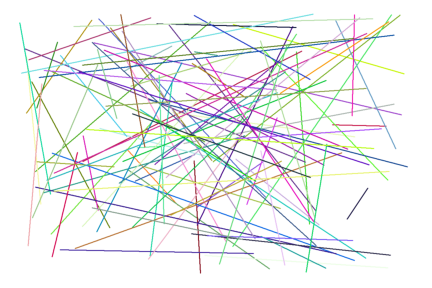
\includegraphics[width=0.5\linewidth]{EMT4Plot2D_Alifia Maylani_23030630039_MatematikaE23-001.png}
    \caption{Enter Caption}
    \label{fig:enter-label}
\end{figure}


\>hold off;

\>window(ow);


Plot dengan beberapa angka dicapai dengan cara yang sama. Ada fungsi
utility figure() untuk ini.


## Plot Aspect

Plot default menggunakan jendela plot persegi. Anda dapat mengubahnya
dengan fungsi aspect(). Jangan lupa untuk mengatur ulang aspeknya
nanti. Anda juga dapat mengubah default ini di menu dengan “Set
Aspect” ke rasio aspek tertentu atau ke ukuran jendela grafik saat
ini.


Tetapi Anda juga dapat mengubahnya untuk satu plot. Untuk ini, ukuran
area plot saat ini diubah, dan jendela diatur sedemikian rupa sehingga
label memiliki ruang yang cukup.


\>aspect(2); // rasio panjang dan lebar 2:1

\>plot2d(["sin(x)","cos(x)"],0,2pi):


\begin{figure}
    \centering
    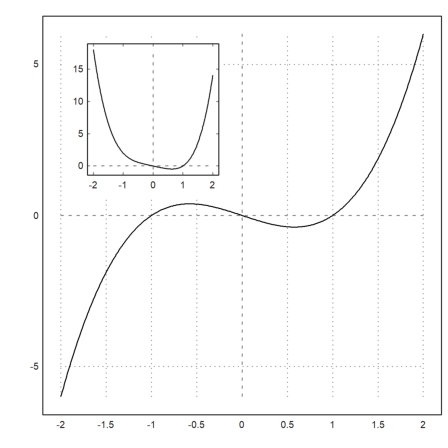
\includegraphics[width=0.5\linewidth]{EMT4Plot2D_Alifia Maylani_23030630039_MatematikaE23-002.png}
    \caption{}
    \label{fig:enter-label}
\end{figure}

\>aspect();

\>reset;


Fungsi reset() mengembalikan default plot, termasuk rasio aspek.


# 2D Plots in Euler

EMT Math Toolbox memiliki plot dalam bentuk 2D, baik untuk data maupun
fungsi. EMT menggunakan fungsi plot2d. Fungsi ini dapat memplot fungsi
dan data.


Dimungkinkan untuk memplot di Maxima menggunakan Gnuplot atau di
Python menggunakan Math Plot Lib.


Euler dapat memplot plot 2D dari


* 
ekspresi

* 
fungsi, variabel, atau kurva berparameter,

* 
vektor nilai x-y,

* 
awan titik-titik di bidang,

* 
kurva implisit dengan level atau wilayah level.

* 
Fungsi yang kompleks


Gaya plot mencakup berbagai gaya untuk garis dan titik, plot batang,
dan plot berbayang.


# Plot Ekspresi atau Variabel

Sebuah ekspresi tunggal dalam “x” (misalnya “4*x^2”) atau nama fungsi
(misalnya “f”) menghasilkan grafik fungsi.


Berikut ini adalah contoh paling dasar, yang menggunakan rentang
default dan menetapkan rentang y yang tepat agar sesuai dengan plot
fungsi.


Catatan: Jika Anda mengakhiri baris perintah dengan tanda titik dua
“:”, plot akan disisipkan ke dalam jendela teks. Jika tidak, tekan TAB
untuk melihat plot jika jendela plot tertutup.


\>plot2d("x^2"):


\begin{figure}
    \centering
    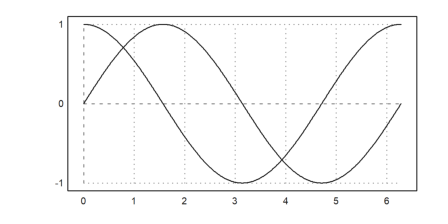
\includegraphics[width=0.5\linewidth]{EMT4Plot2D_Alifia Maylani_23030630039_MatematikaE23-003.png}
    \caption{}
    \label{fig:enter-label}
\end{figure}

\>aspect(1.5); plot2d("x^3-x"):


\begin{figure}
    \centering
    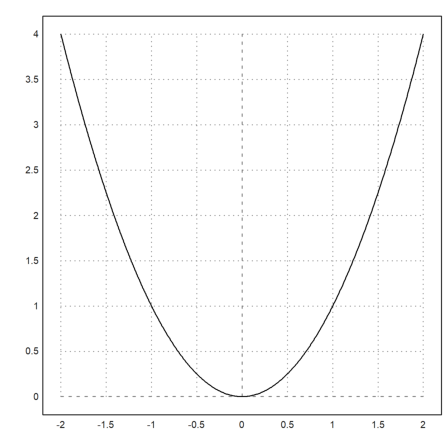
\includegraphics[width=0.5\linewidth]{EMT4Plot2D_Alifia Maylani_23030630039_MatematikaE23-004.png}
    \caption{}
    \label{fig:enter-label}
\end{figure}

\>a:=5.6; plot2d("exp(-a\*x^2)/a"); insimg(30); // menampilkan gambar hasil plot setinggi 25 baris


\begin{figure}
    \centering
    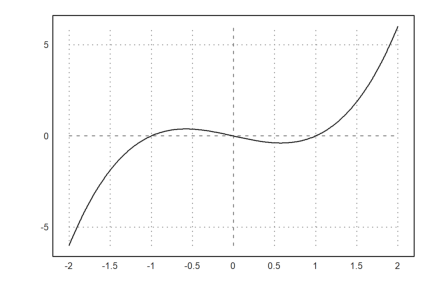
\includegraphics[width=0.5\linewidth]{EMT4Plot2D_Alifia Maylani_23030630039_MatematikaE23-005.png}
    \caption{}
    \label{fig:enter-label}
\end{figure}

Dari beberapa contoh sebelumnya Anda dapat melihat bahwa aslinya
gambar plot menggunakan sumbu X dengan rentang nilai dari -2 sampai
dengan 2. Untuk mengubah rentang nilai X dan Y, Anda dapat menambahkan
nilai-nilai batas X (dan Y) di belakang ekspresi yang digambar.


Rentang plot ditetapkan dengan parameter yang ditetapkan berikut ini


* 
a,b: rentang x (default -2,2)

* 
c, d: rentang y (default: skala dengan nilai)

* 
r: sebagai alternatif, radius di sekitar pusat plot

* 
cx, cy: koordinat pusat plot (default 0,0)


\>plot2d("x^3-x",-1,2):


\begin{figure}
    \centering
    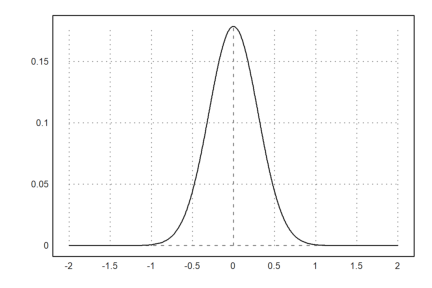
\includegraphics[width=0.5\linewidth]{EMT4Plot2D_Alifia Maylani_23030630039_MatematikaE23-006.png}
    \caption{}
    \label{fig:enter-label}
\end{figure}

\>plot2d("sin(x)",-2\*pi,2\*pi): // plot sin(x) pada interval [-2pi, 2pi]


\begin{figure}
    \centering
    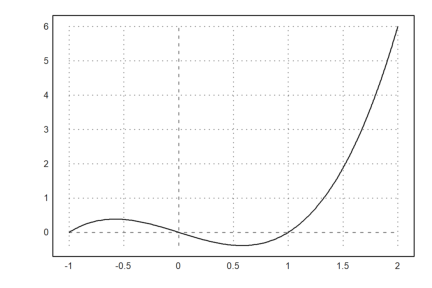
\includegraphics[width=0.5\linewidth]{EMT4Plot2D_Alifia Maylani_23030630039_MatematikaE23-007.png}
    \caption{}
    \label{fig:enter-label}
\end{figure}

\>plot2d("cos(x)","sin(3\*x)",xmin=0,xmax=2pi):


\begin{figure}
    \centering
    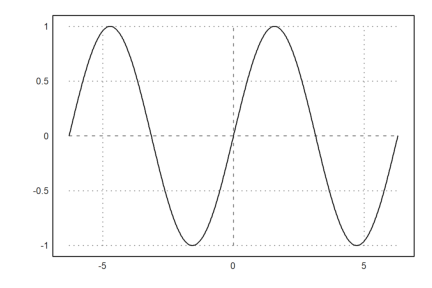
\includegraphics[width=0.5\linewidth]{EMT4Plot2D_Alifia Maylani_23030630039_MatematikaE23-008.png}
    \caption{}
    \label{fig:enter-label}
\end{figure}

Alternatif untuk tanda titik dua adalah perintah insimg(lines), yang
menyisipkan plot yang menempati sejumlah baris teks tertentu.


Dalam opsi, plot dapat diatur untuk muncul


* 
di jendela terpisah yang dapat diubah ukurannya,

* 
di jendela buku catatan.


Lebih banyak gaya yang dapat dicapai dengan perintah plot tertentu.


Dalam hal apa pun, tekan tombol tabulator untuk melihat plot, jika
disembunyikan.


Untuk membagi jendela menjadi beberapa plot, gunakan perintah
figure(). Pada contoh, kita memplot x^1 sampai x^4 ke dalam 4 bagian
jendela. figure(0) akan mereset jendela default.


\>reset;

\>figure(2,2); ...  
\>   for n=1 to 4; figure(n); plot2d("x^"+n); end; ...  
\>   figure(0):


\begin{figure}
    \centering
    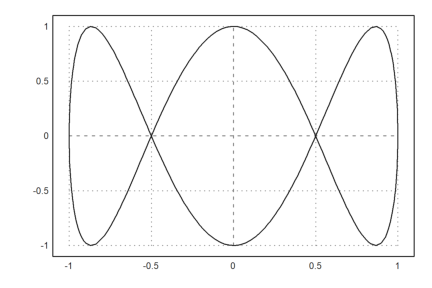
\includegraphics[width=0.5\linewidth]{EMT4Plot2D_Alifia Maylani_23030630039_MatematikaE23-009.png}
    \caption{}
    \label{fig:enter-label}
\end{figure}

In plot2d(), there are alternative styles available with grid=x. For an overview, we
show the various grid styles in one figure (see below for the figure() command). The
style grid=0 is not included. It shows no grid and no frame.


\>figure(3,3); ...  
\>   for k=1:9; figure(k); plot2d("x^3-x",-2,1,grid=k); end; ...  
\>   figure(0):


\begin{figure}
    \centering
    \includegraphics[width=0.5\linewidth]{EMT4Plot2D_Alifia Maylani_23030630039_MatematikaE23-010.png}
    \caption{}
    \label{fig:enter-label}
\end{figure}

Jika argumen untuk plot2d() adalah sebuah ekspresi yang diikuti oleh
empat angka, angka-angka ini adalah rentang x dan y untuk plot.


Atau, a, b, c, d dapat ditentukan sebagai parameter yang ditetapkan
sebagai a=... dst.


Pada contoh berikut, kita mengubah gaya grid, menambahkan label, dan
menggunakan label vertikal untuk sumbu y.


\>aspect(1.5); plot2d("sin(x)",0,2pi,-1.2,1.2,grid=3,xl="x",yl="sin(x)"):


\begin{figure}
    \centering
    \includegraphics[width=0.5\linewidth]{EMT4Plot2D_Alifia Maylani_23030630039_MatematikaE23-011.png}
    \caption{}
    \label{fig:enter-label}
\end{figure}

\>plot2d("sin(x)+cos(2\*x)",0,4pi):


\begin{figure}
    \centering
    \includegraphics[width=0.5\linewidth]{EMT4Plot2D_Alifia Maylani_23030630039_MatematikaE23-012.png}
    \caption{}
    \label{fig:enter-label}
\end{figure}

Gambar yang dihasilkan dengan menyisipkan plot ke dalam jendela teks
disimpan dalam direktori yang sama dengan notebook, secara default
dalam subdirektori bernama “images”. Gambar-gambar tersebut juga
digunakan oleh ekspor HTML.


Anda cukup menandai gambar mana saja dan menyalinnya ke clipboard
dengan Ctrl-C. Tentu saja, Anda juga dapat mengekspor grafik saat ini
dengan fungsi-fungsi pada menu File.


Fungsi atau ekspresi dalam plot2d dievaluasi secara adaptif. Untuk
kecepatan yang lebih tinggi, matikan plot adaptif dengan &lt;adaptive dan
tentukan jumlah subinterval dengan n=... Hal ini hanya diperlukan pada
kasus-kasus yang jarang terjadi.


\>plot2d("sign(x)\*exp(-x^2)",-1,1,<adaptive,n=10000):

\begin{figure}
    \centering
    \includegraphics[width=0.5\linewidth]{EMT4Plot2D_Alifia Maylani_23030630039_MatematikaE23-013.png}
    \caption{}
    \label{fig:enter-label}
\end{figure}

\>plot2d("x^x",r=1.2,cx=1,cy=1):


\begin{figure}
    \centering
    \includegraphics[width=0.5\linewidth]{EMT4Plot2D_Alifia Maylani_23030630039_MatematikaE23-014.png}
    \caption{}
    \label{fig:enter-label}
\end{figure}

Perhatikan bahwa x^x tidak didefinisikan untuk x&lt;=0. Fungsi plot2d
menangkap kesalahan ini, dan mulai memplot segera setelah fungsi
didefinisikan. Hal ini berlaku untuk semua fungsi yang mengembalikan
NAN di luar jangkauan definisinya.


\>plot2d("log(x)",-0.1,2):


\begin{figure}
    \centering
    \includegraphics[width=0.5\linewidth]{EMT4Plot2D_Alifia Maylani_23030630039_MatematikaE23-015.png}
    \caption{}
    \label{fig:enter-label}
\end{figure}

Parameter square=true (atau &gt;square) memilih rentang y secara otomatis
sehingga hasilnya adalah jendela plot persegi. Perhatikan bahwa secara
default, Euler menggunakan ruang persegi di dalam jendela plot.


\>plot2d("x^3-x",\>square):


\begin{figure}
    \centering
    \includegraphics[width=0.5\linewidth]{EMT4Plot2D_Alifia Maylani_23030630039_MatematikaE23-016.png}
    \caption{}
    \label{fig:enter-label}
\end{figure}

\>plot2d(''integrate("sin(x)\*exp(-x^2)",0,x)'',0,2): // plot integral


\begin{figure}
    \centering
    \includegraphics[width=0.5\linewidth]{EMT4Plot2D_Alifia Maylani_23030630039_MatematikaE23-017.png}
    \caption{}
    \label{fig:enter-label}
\end{figure}

Jika Anda membutuhkan lebih banyak ruang untuk label-y, panggil
shrinkwindow() dengan parameter lebih kecil, atau tetapkan nilai
positif untuk “lebih kecil” pada plot2d().


\>plot2d("gamma(x)",1,10,yl="y-values",smaller=6,<vertical):


\begin{figure}
    \centering
    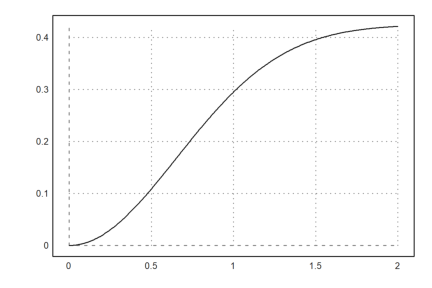
\includegraphics[width=0.5\linewidth]{EMT4Plot2D_Alifia Maylani_23030630039_MatematikaE23-018.png}
    \caption{}
    \label{fig:enter-label}
\end{figure}

Ekspresi simbolik juga dapat digunakan, karena disimpan sebagai
ekspresi string sederhana.


\>x=linspace(0,2pi,1000); plot2d(sin(5x),cos(7x)):


\begin{figure}
    \centering
    \includegraphics[width=0.5\linewidth]{EMT4Plot2D_Alifia Maylani_23030630039_MatematikaE23-019.png}
    \caption{}
    \label{fig:enter-label}
\end{figure}

\>a:=5.6; expr &= exp(-a\*x^2)/a; // define expression

\>plot2d(expr,-2,2): // plot from -2 to 2


\begin{figure}
    \centering
    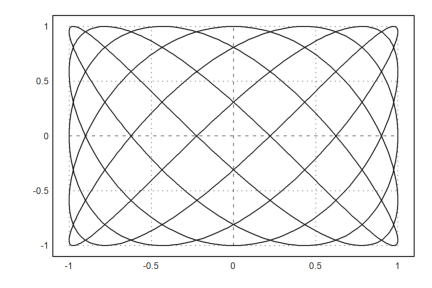
\includegraphics[width=0.5\linewidth]{EMT4Plot2D_Alifia Maylani_23030630039_MatematikaE23-020.png}
    \caption{}
    \label{fig:enter-label}
\end{figure}

\>plot2d(expr,r=1,thickness=2): // plot in a square around (0,0)


![images/EMT4Plot2D_Alifia%20Maylani_23030630039_MatematikaE23-022.png](images/EMT4Plot2D_Alifia%20Maylani_23030630039_MatematikaE23-022.png)

\>plot2d(&diff(expr,x),\>add,style="--",color=red): // add another plot


![images/EMT4Plot2D_Alifia%20Maylani_23030630039_MatematikaE23-023.png](images/EMT4Plot2D_Alifia%20Maylani_23030630039_MatematikaE23-023.png)

\>plot2d(&diff(expr,x,2),a=-2,b=2,c=-2,d=1): // plot in rectangle


![images/EMT4Plot2D_Alifia%20Maylani_23030630039_MatematikaE23-024.png](images/EMT4Plot2D_Alifia%20Maylani_23030630039_MatematikaE23-024.png)

\>plot2d(&diff(expr,x),a=-2,b=2,\>square): // keep plot square


![images/EMT4Plot2D_Alifia%20Maylani_23030630039_MatematikaE23-025.png](images/EMT4Plot2D_Alifia%20Maylani_23030630039_MatematikaE23-025.png)

\>plot2d("x^2",0,1,steps=1,color=red,n=10):


![images/EMT4Plot2D_Alifia%20Maylani_23030630039_MatematikaE23-026.png](images/EMT4Plot2D_Alifia%20Maylani_23030630039_MatematikaE23-026.png)

\>plot2d("x^2",\>add,steps=2,color=blue,n=10):


![images/EMT4Plot2D_Alifia%20Maylani_23030630039_MatematikaE23-027.png](images/EMT4Plot2D_Alifia%20Maylani_23030630039_MatematikaE23-027.png)

# Functions in one Parameter (Fungsi dalam satu Parameter)

Fungsi plot yang paling penting untuk plot planar adalah plot2d().
Fungsi ini diimplementasikan dalam bahasa Euler dalam file “plot.e”,
yang dimuat pada awal program.


Berikut adalah beberapa contoh penggunaan fungsi. Seperti biasa dalam
EMT, fungsi yang bekerja untuk fungsi atau ekspresi lain, Anda dapat
mengoper parameter tambahan (selain x) yang bukan variabel global ke
fungsi dengan parameter titik koma atau dengan koleksi panggilan.


\>function f(x,a) := x^2/a+a\*x^2-x; // define a function

\>a=0.3; plot2d("f",0,1;a): // plot with a=0.3


![images/EMT4Plot2D_Alifia%20Maylani_23030630039_MatematikaE23-028.png](images/EMT4Plot2D_Alifia%20Maylani_23030630039_MatematikaE23-028.png)

\>plot2d("f",0,1;0.4): // plot with a=0.4


![images/EMT4Plot2D_Alifia%20Maylani_23030630039_MatematikaE23-029.png](images/EMT4Plot2D_Alifia%20Maylani_23030630039_MatematikaE23-029.png)

\>plot2d({{"f",0.2}},0,1): // plot with a=0.2


![images/EMT4Plot2D_Alifia%20Maylani_23030630039_MatematikaE23-030.png](images/EMT4Plot2D_Alifia%20Maylani_23030630039_MatematikaE23-030.png)

\>plot2d({{"f(x,b)",b=0.1}},0,1): // plot with 0.1


![images/EMT4Plot2D_Alifia%20Maylani_23030630039_MatematikaE23-031.png](images/EMT4Plot2D_Alifia%20Maylani_23030630039_MatematikaE23-031.png)

\>function f(x) := x^3-x; ...  
\>   plot2d("f",r=1):


![images/EMT4Plot2D_Alifia%20Maylani_23030630039_MatematikaE23-032.png](images/EMT4Plot2D_Alifia%20Maylani_23030630039_MatematikaE23-032.png)

Berikut ini adalah ringkasan dari fungsi yang diterima


* 
ekspresi atau ekspresi simbolik dalam x

* 
fungsi atau fungsi simbolik dengan nama sebagai “f”

* 
fungsi-fungsi simbolik hanya dengan nama f


Fungsi plot2d() juga menerima fungsi simbolik. Untuk fungsi simbolik,
nama saja sudah cukup.


\>function f(x) &= diff(x^x,x)


    
                                x
                               x  (log(x) + 1)
    

\>plot2d(f,0,2):


![images/EMT4Plot2D_Alifia%20Maylani_23030630039_MatematikaE23-033.png](images/EMT4Plot2D_Alifia%20Maylani_23030630039_MatematikaE23-033.png)

Tentu saja, untuk ekspresi atau ungkapan simbolik, nama variabel sudah
cukup untuk memplotnya.


\>expr &= sin(x)\*exp(-x)


    
                                  - x
                                 E    sin(x)
    

\>plot2d(expr,0,3pi):


![images/EMT4Plot2D_Alifia%20Maylani_23030630039_MatematikaE23-034.png](images/EMT4Plot2D_Alifia%20Maylani_23030630039_MatematikaE23-034.png)

\>function f(x) &= x^x;

\>plot2d(f,r=1,cx=1,cy=1,color=blue,thickness=2);

\>plot2d(&diff(f(x),x),\>add,color=red,style="-.-"):


![images/EMT4Plot2D_Alifia%20Maylani_23030630039_MatematikaE23-035.png](images/EMT4Plot2D_Alifia%20Maylani_23030630039_MatematikaE23-035.png)

Untuk gaya garis, ada berbagai pilihan.


* 
style = “...”. Pilih dari “-”, “--”, “-.”, “.”, “.-.”, “-.-”.

* 
color: Lihat di bawah untuk warna.

* 
ketebalan: Default adalah 1.


Warna dapat dipilih sebagai salah satu warna default, atau sebagai
warna RGB.


* 
0..15: indeks warna default.

* 
konstanta warna: putih, hitam, merah, hijau, biru, cyan, zaitun,
* abu-abu muda, abu-abu, abu-abu tua, oranye, hijau muda, pirus, biru
* muda, oranye muda, kuning

* 
rgb (merah, hijau, biru): parameter adalah real dalam [0,1].


\>plot2d("exp(-x^2)",r=2,color=red,thickness=3,style="--"):


![images/EMT4Plot2D_Alifia%20Maylani_23030630039_MatematikaE23-036.png](images/EMT4Plot2D_Alifia%20Maylani_23030630039_MatematikaE23-036.png)

Berikut ini adalah pemandangan warna EMT yang sudah ditetapkan
sebelumnya.


\>aspect(2); columnsplot(ones(1,16),lab=0:15,grid=0,color=0:15):


![images/EMT4Plot2D_Alifia%20Maylani_23030630039_MatematikaE23-037.png](images/EMT4Plot2D_Alifia%20Maylani_23030630039_MatematikaE23-037.png)

Tetapi Anda bisa menggunakan warna apa pun.


\>columnsplot(ones(1,16),grid=0,color=rgb(0,0,linspace(0,1,15))):


![images/EMT4Plot2D_Alifia%20Maylani_23030630039_MatematikaE23-038.png](images/EMT4Plot2D_Alifia%20Maylani_23030630039_MatematikaE23-038.png)

# Menggambar Beberapa Kurva pada bidang koordinat yang sama

Memplot lebih dari satu fungsi (beberapa fungsi) ke dalam satu jendela
dapat dilakukan dengan berbagai cara. Salah satu caranya adalah dengan
menggunakan &gt;add untuk beberapa pemanggilan ke plot2d secara
bersamaan, kecuali pemanggilan pertama. Kita telah menggunakan fitur
ini pada contoh di atas.


\>aspect(); plot2d("cos(x)",r=2,grid=6); plot2d("x",style=".",\>add):


![images/EMT4Plot2D_Alifia%20Maylani_23030630039_MatematikaE23-039.png](images/EMT4Plot2D_Alifia%20Maylani_23030630039_MatematikaE23-039.png)

\>aspect(1.5); plot2d("sin(x)",0,2pi); plot2d("cos(x)",color=blue,style="--",\>add):


![images/EMT4Plot2D_Alifia%20Maylani_23030630039_MatematikaE23-040.png](images/EMT4Plot2D_Alifia%20Maylani_23030630039_MatematikaE23-040.png)

Salah satu kegunaan &gt;add adalah untuk menambahkan titik pada kurva.


\>plot2d("sin(x)",0,pi); plot2d(2,sin(2),\>points,\>add):


![images/EMT4Plot2D_Alifia%20Maylani_23030630039_MatematikaE23-041.png](images/EMT4Plot2D_Alifia%20Maylani_23030630039_MatematikaE23-041.png)

Kami menambahkan titik perpotongan dengan label (pada posisi “cl”
untuk kiri tengah), dan menyisipkan hasilnya ke dalam buku catatan.
Kami juga menambahkan judul ke plot.


\>plot2d(["cos(x)","x"],r=1.1,cx=0.5,cy=0.5, ...  
\>     color=[black,blue],style=["-","."], ...  
\>     grid=1);

\>x0=solve("cos(x)-x",1);  ...  
\>     plot2d(x0,x0,\>points,\>add,title="Intersection Demo");  ...  
\>     label("cos(x) = x",x0,x0,pos="cl",offset=20):


![images/EMT4Plot2D_Alifia%20Maylani_23030630039_MatematikaE23-042.png](images/EMT4Plot2D_Alifia%20Maylani_23030630039_MatematikaE23-042.png)

Dalam demo berikut ini, kami memplot fungsi sinc(x)=sin(x)/x dan
ekspansi Taylor ke-8 dan ke-16. Kami menghitung ekspansi ini
menggunakan Maxima melalui ekspresi simbolik.


Plot ini dilakukan dalam perintah multi-baris berikut dengan tiga
pemanggilan plot2d(). Perintah kedua dan ketiga memiliki set flag
&gt;add, yang membuat plot menggunakan rentang sebelumnya.


Kami menambahkan sebuah kotak label yang menjelaskan fungsi-fungsi
tersebut.


\>$taylor(sin(x)/x,x,0,4)


$$\frac{x^4}{120}-\frac{x^2}{6}+1$$\>plot2d("sinc(x)",0,4pi,color=green,thickness=2); ...  
\>     plot2d(&taylor(sin(x)/x,x,0,8),\>add,color=blue,style="--"); ...  
\>     plot2d(&taylor(sin(x)/x,x,0,16),\>add,color=red,style="-.-"); ...  
\>     labelbox(["sinc","T8","T16"],styles=["-","--","-.-"], ...  
\>       colors=[black,blue,red]):


![images/EMT4Plot2D_Alifia%20Maylani_23030630039_MatematikaE23-044.png](images/EMT4Plot2D_Alifia%20Maylani_23030630039_MatematikaE23-044.png)

Pada contoh berikut, kami menghasilkan Polinomial Bernstein.


$$B_i(x) = \binom{n}{i} x^i (1-x)^{n-i}$$\>plot2d("(1-x)^10",0,1); // plot first function

\>for i=1 to 10; plot2d("bin(10,i)\*x^i\*(1-x)^(10-i)",\>add); end;

\>insimg;


![images/EMT4Plot2D_Alifia%20Maylani_23030630039_MatematikaE23-046.png](images/EMT4Plot2D_Alifia%20Maylani_23030630039_MatematikaE23-046.png)

Metode kedua menggunakan sepasang matriks nilai x dan matriks nilai y
dengan ukuran yang sama.


Kita membuat sebuah matriks nilai dengan satu Polinomial Bernstein di
setiap baris. Untuk ini, kita cukup menggunakan vektor kolom i.
Lihatlah pengantar tentang bahasa matriks untuk mempelajari lebih
lanjut.


\>x=linspace(0,1,500);

\>n=10; k=(0:n)'; // n is row vector, k is column vector

\>y=bin(n,k)\*x^k\*(1-x)^(n-k); // y is a matrix then

\>plot2d(x,y):


![images/EMT4Plot2D_Alifia%20Maylani_23030630039_MatematikaE23-047.png](images/EMT4Plot2D_Alifia%20Maylani_23030630039_MatematikaE23-047.png)

Perhatikan bahwa parameter warna dapat berupa vektor. Kemudian setiap
warna digunakan untuk setiap baris matriks.


\>x=linspace(0,1,200); y=x^(1:10)'; plot2d(x,y,color=1:10):


![images/EMT4Plot2D_Alifia%20Maylani_23030630039_MatematikaE23-048.png](images/EMT4Plot2D_Alifia%20Maylani_23030630039_MatematikaE23-048.png)

Metode lainnya adalah menggunakan vektor ekspresi (string). Anda
kemudian dapat menggunakan larik warna, larik gaya, dan larik
ketebalan dengan panjang yang sama.


\>plot2d(["sin(x)","cos(x)"],0,2pi,color=4:5): 


![images/EMT4Plot2D_Alifia%20Maylani_23030630039_MatematikaE23-049.png](images/EMT4Plot2D_Alifia%20Maylani_23030630039_MatematikaE23-049.png)

\>plot2d(["sin(x)","cos(x)"],0,2pi): // plot vector of expressions


![images/EMT4Plot2D_Alifia%20Maylani_23030630039_MatematikaE23-050.png](images/EMT4Plot2D_Alifia%20Maylani_23030630039_MatematikaE23-050.png)

Kita bisa mendapatkan vektor seperti itu dari Maxima dengan
menggunakan makelist() dan mxm2str().


\>v &= makelist(binomial(10,i)\*x^i\*(1-x)^(10-i),i,0,10) // make list


    
                   10            9              8  2             7  3
           [(1 - x)  , 10 (1 - x)  x, 45 (1 - x)  x , 120 (1 - x)  x , 
               6  4             5  5             4  6             3  7
    210 (1 - x)  x , 252 (1 - x)  x , 210 (1 - x)  x , 120 (1 - x)  x , 
              2  8              9   10
    45 (1 - x)  x , 10 (1 - x) x , x  ]
    

\>mxm2str(v) // get a vector of strings from the symbolic vector


    (1-x)^10
    10*(1-x)^9*x
    45*(1-x)^8*x^2
    120*(1-x)^7*x^3
    210*(1-x)^6*x^4
    252*(1-x)^5*x^5
    210*(1-x)^4*x^6
    120*(1-x)^3*x^7
    45*(1-x)^2*x^8
    10*(1-x)*x^9
    x^10

\>plot2d(mxm2str(v),0,1): // plot functions


![images/EMT4Plot2D_Alifia%20Maylani_23030630039_MatematikaE23-051.png](images/EMT4Plot2D_Alifia%20Maylani_23030630039_MatematikaE23-051.png)

Alternatif lain adalah dengan menggunakan bahasa matriks Euler.


Jika sebuah ekspresi menghasilkan sebuah matriks fungsi, dengan satu
fungsi di setiap baris, semua fungsi ini akan diplot ke dalam satu
plot.


Untuk ini, gunakan vektor parameter dalam bentuk vektor kolom. Jika
sebuah larik warna ditambahkan, maka akan digunakan untuk setiap baris
plot.


\>n=(1:10)'; plot2d("x^n",0,1,color=1:10):


![images/EMT4Plot2D_Alifia%20Maylani_23030630039_MatematikaE23-052.png](images/EMT4Plot2D_Alifia%20Maylani_23030630039_MatematikaE23-052.png)

Ekspresi dan fungsi satu baris dapat melihat variabel global.


Jika Anda tidak dapat menggunakan variabel global, Anda perlu
menggunakan fungsi dengan parameter tambahan, dan memberikan parameter
ini sebagai parameter titik koma.


Berhati-hatilah untuk meletakkan semua parameter yang diberikan di
akhir perintah plot2d. Pada contoh ini kita mengoper a=5 ke fungsi f,
yang kita plot dari -10 ke 10.


\>function f(x,a) := 1/a\*exp(-x^2/a); ...  
\>   plot2d("f",-10,10;5,thickness=2,title="a=5"):


![images/EMT4Plot2D_Alifia%20Maylani_23030630039_MatematikaE23-053.png](images/EMT4Plot2D_Alifia%20Maylani_23030630039_MatematikaE23-053.png)

Atau, gunakan koleksi dengan nama fungsi dan semua parameter tambahan.
Daftar khusus ini disebut koleksi panggilan, dan itu adalah cara yang
lebih disukai untuk mengoper argumen ke fungsi yang dengan sendirinya
dioper sebagai argumen ke fungsi lain.


Pada contoh berikut, kita menggunakan perulangan untuk memplot
beberapa fungsi (lihat tutorial tentang pemrograman perulangan).


\>plot2d({{"f",1}},-10,10); ...  
\>   for a=2:10; plot2d({{"f",a}},\>add); end:


![images/EMT4Plot2D_Alifia%20Maylani_23030630039_MatematikaE23-054.png](images/EMT4Plot2D_Alifia%20Maylani_23030630039_MatematikaE23-054.png)

Kita dapat mencapai hasil yang sama dengan cara berikut menggunakan
bahasa matriks EMT. Setiap baris dari matriks f(x,a) adalah satu
fungsi. Selain itu, kita dapat mengatur warna untuk setiap baris
matriks. Klik dua kali pada fungsi getspectral() untuk penjelasannya.


\>x=-10:0.01:10; a=(1:10)'; plot2d(x,f(x,a),color=getspectral(a/10)):


![images/EMT4Plot2D_Alifia%20Maylani_23030630039_MatematikaE23-055.png](images/EMT4Plot2D_Alifia%20Maylani_23030630039_MatematikaE23-055.png)

## Text Labels

Dekorasi sederhana dapat berupa


* 
sebuah judul dengan title=”...”

* 
label x dan y dengan xl=“...”, yl=”...”

* 
label teks lain dengan label(“...”,x,y)


Perintah label akan memplotkan ke dalam plot saat ini pada koordinat
plot (x,y). Perintah ini dapat menerima sebuah argumen posisi.


\>plot2d("x^3-x",-1,2,title="y=x^3-x",yl="y",xl="x"):


![images/EMT4Plot2D_Alifia%20Maylani_23030630039_MatematikaE23-056.png](images/EMT4Plot2D_Alifia%20Maylani_23030630039_MatematikaE23-056.png)

\>expr := "log(x)/x"; ...  
\>     plot2d(expr,0.5,5,title="y="+expr,xl="x",yl="y"); ...  
\>     label("(1,0)",1,0); label("Max",E,expr(E),pos="lc"):


![images/EMT4Plot2D_Alifia%20Maylani_23030630039_MatematikaE23-057.png](images/EMT4Plot2D_Alifia%20Maylani_23030630039_MatematikaE23-057.png)

Ada juga fungsi labelbox(), yang dapat menampilkan fungsi dan teks.
Fungsi ini membutuhkan vektor string dan warna, satu item untuk setiap
fungsi.


\>function f(x) &= x^2\*exp(-x^2);  ...  
\>   plot2d(&f(x),a=-3,b=3,c=-1,d=1);  ...  
\>   plot2d(&diff(f(x),x),\>add,color=blue,style="--"); ...  
\>   labelbox(["function","derivative"],styles=["-","--"], ...  
\>      colors=[black,blue],w=0.4):


![images/EMT4Plot2D_Alifia%20Maylani_23030630039_MatematikaE23-058.png](images/EMT4Plot2D_Alifia%20Maylani_23030630039_MatematikaE23-058.png)

Kotak tersebut berlabuh di kanan atas secara default, tetapi &gt;kiri
menambatkannya di kiri atas. Anda dapat memindahkannya ke tempat mana
pun yang Anda suka. Posisi jangkar adalah sudut kanan atas kotak, dan
angkanya adalah pecahan dari ukuran jendela grafik. Lebarnya otomatis.


Untuk plot titik, kotak label juga dapat digunakan. Tambahkan
parameter &gt;titik, atau vektor bendera, satu untuk setiap label.


Pada contoh berikut, hanya ada satu fungsi. Jadi kita dapat
menggunakan string sebagai pengganti vektor string. Kita mengatur
warna teks menjadi hitam untuk contoh ini.


\>n=10; plot2d(0:n,bin(n,0:n),\>addpoints); ...  
\>   labelbox("Binomials",styles="[]",\>points,x=0.1,y=0.1, ...  
\>   tcolor=black,\>left):


![images/EMT4Plot2D_Alifia%20Maylani_23030630039_MatematikaE23-059.png](images/EMT4Plot2D_Alifia%20Maylani_23030630039_MatematikaE23-059.png)

Gaya plot ini juga tersedia di statplot(). Seperti pada plot2d() warna
dapat diatur untuk setiap baris plot. Terdapat lebih banyak plot
khusus untuk keperluan statistik (lihat tutorial tentang statistik).


\>statplot(1:10,random(2,10),color=[red,blue]):


![images/EMT4Plot2D_Alifia%20Maylani_23030630039_MatematikaE23-060.png](images/EMT4Plot2D_Alifia%20Maylani_23030630039_MatematikaE23-060.png)

Fitur yang serupa adalah fungsi textbox().


Lebarnya secara default adalah lebar maksimal baris teks. Tetapi bisa
juga diatur oleh pengguna.


\>function f(x) &= exp(-x)\*sin(2\*pi\*x); ...  
\>   plot2d("f(x)",0,2pi); ...  
\>   textbox(latex("\\text{Example of a damped oscillation}\\ f(x)=e^{-x}sin(2\\pi x)"),w=0.85):


![images/EMT4Plot2D_Alifia%20Maylani_23030630039_MatematikaE23-061.png](images/EMT4Plot2D_Alifia%20Maylani_23030630039_MatematikaE23-061.png)

Label teks, judul, kotak label, dan teks lainnya dapat berisi string
Unicode (lihat sintaks EMT untuk mengetahui lebih lanjut tentang
string Unicode).


\>plot2d("x^3-x",title=u"x &rarr; x&sup3; - x"):


![images/EMT4Plot2D_Alifia%20Maylani_23030630039_MatematikaE23-062.png](images/EMT4Plot2D_Alifia%20Maylani_23030630039_MatematikaE23-062.png)

Label pada sumbu x dan y bisa vertikal, begitu juga dengan sumbu.


\>plot2d("sinc(x)",0,2pi,xl="x",yl=u"x &rarr; sinc(x)",\>vertical):


![images/EMT4Plot2D_Alifia%20Maylani_23030630039_MatematikaE23-063.png](images/EMT4Plot2D_Alifia%20Maylani_23030630039_MatematikaE23-063.png)

## LaTeX

Anda juga dapat memplot formula LaTeX jika Anda telah menginstal
sistem LaTeX. Saya merekomendasikan MiKTeX. Jalur ke binari “lateks”
dan “dvipng” harus berada di jalur sistem, atau Anda harus mengatur
LaTeX di menu opsi.


Perhatikan, bahwa penguraian LaTeX berjalan lambat. Jika Anda ingin
menggunakan LaTeX dalam plot animasi, Anda harus memanggil latex()
sebelum perulangan satu kali dan menggunakan hasilnya (gambar dalam
matriks RGB).


Pada plot berikut ini, kita menggunakan LaTeX untuk label x dan y,
sebuah label, kotak label dan judul plot.


\>plot2d("exp(-x)\*sin(x)/x",a=0,b=2pi,c=0,d=1,grid=6,color=blue, ...  
\>     title=latex("\\text{Function $\\Phi$}"), ...  
\>     xl=latex("\\phi"),yl=latex("\\Phi(\\phi)")); ...  
\>   textbox( ...  
\>     latex("\\Phi(\\phi) = e^{-\\phi} \\frac{\\sin(\\phi)}{\\phi}"),x=0.8,y=0.5); ...  
\>   label(latex("\\Phi",color=blue),1,0.4):


![images/EMT4Plot2D_Alifia%20Maylani_23030630039_MatematikaE23-064.png](images/EMT4Plot2D_Alifia%20Maylani_23030630039_MatematikaE23-064.png)

Seringkali, kita menginginkan spasi dan label teks yang tidak sesuai
pada sumbu x. Kita dapat menggunakan xaxis() dan yaxis() seperti yang
akan kita tunjukkan nanti.


Cara termudah adalah dengan membuat plot kosong dengan sebuah frame
menggunakan grid=4, dan kemudian menambahkan grid dengan ygrid() dan
xgrid(). Pada contoh berikut, kita menggunakan tiga buah string LaTeX
untuk label pada sumbu x dengan xtick().


\>plot2d("sinc(x)",0,2pi,grid=4,<ticks); ...  
\>   ygrid(-2:0.5:2,grid=6); ...  
\>   xgrid([0:2]\*pi,<ticks,grid=6);  ...  
\>   xtick([0,pi,2pi],["0","\\pi","2\\pi"],\>latex):


![images/EMT4Plot2D_Alifia%20Maylani_23030630039_MatematikaE23-065.png](images/EMT4Plot2D_Alifia%20Maylani_23030630039_MatematikaE23-065.png)

Tentu saja, fungsi juga dapat digunakan.


\>function map f(x) ...


    if x>0 then return x^4
    else return x^2
    endif
    endfunction
</pre>
Parameter “map” membantu menggunakan fungsi untuk vektor. Untuk


plot, hal ini tidak diperlukan. Tetapi untuk mendemonstrasikan bahwa
vektorisasi


berguna, kami menambahkan beberapa titik kunci pada plot pada x=-1,
x=0 dan x=1.


Pada plot berikut, kita juga memasukkan beberapa kode LaTeX. Kita
menggunakannya untuk


dua label dan sebuah kotak teks. Tentu saja, Anda hanya dapat
menggunakan


LaTeX jika Anda telah menginstal LaTeX dengan benar.


\>plot2d("f",-1,1,xl="x",yl="f(x)",grid=6);  ...  
\>   plot2d([-1,0,1],f([-1,0,1]),\>points,\>add); ...  
\>   label(latex("x^3"),0.72,f(0.72)); ...  
\>   label(latex("x^2"),-0.52,f(-0.52),pos="ll"); ...  
\>   textbox( ...  
\>     latex("f(x)=\\begin{cases} x^3 & x\>0 \\\\ x^2 & x \\le 0\\end{cases}"), ...  
\>     x=0.7,y=0.2):


![images/EMT4Plot2D_Alifia%20Maylani_23030630039_MatematikaE23-066.png](images/EMT4Plot2D_Alifia%20Maylani_23030630039_MatematikaE23-066.png)

## User Interaction (Interaksi Pengguna)

Ketika memplot fungsi atau ekspresi, parameter &gt;user memungkinkan
pengguna untuk memperbesar dan menggeser plot dengan tombol kursor
atau mouse. Pengguna dapat


* 
memperbesar dengan + atau -

* 
memindahkan plot dengan tombol kursor

* 
memilih jendela plot dengan mouse

* 
mengatur ulang tampilan dengan spasi

* 
keluar dengan return


Tombol spasi akan mengatur ulang plot ke jendela plot awal.


Ketika memplot data, bendera &gt;user hanya akan menunggu penekanan
tombol.


\>plot2d({{"x^3-a\*x",a=1}},\>user,title="Press any key!"):


![images/EMT4Plot2D_Alifia%20Maylani_23030630039_MatematikaE23-067.png](images/EMT4Plot2D_Alifia%20Maylani_23030630039_MatematikaE23-067.png)

\>plot2d("exp(x)\*sin(x)",user=true, ...  
\>     title="+/- or cursor keys (return to exit)"):


![images/EMT4Plot2D_Alifia%20Maylani_23030630039_MatematikaE23-068.png](images/EMT4Plot2D_Alifia%20Maylani_23030630039_MatematikaE23-068.png)

Berikut ini menunjukkan cara interaksi pengguna tingkat lanjut (lihat
tutorial tentang pemrograman untuk detailnya).


Fungsi bawaan mousedrag() menunggu peristiwa mouse atau keyboard.
Fungsi ini melaporkan mouse ke bawah, mouse bergerak atau mouse ke
atas, dan penekanan tombol. Fungsi dragpoints() memanfaatkan hal ini,
dan mengizinkan pengguna untuk menyeret titik manapun di dalam plot.


Kita membutuhkan fungsi plot terlebih dahulu. Sebagai contoh, kita
melakukan interpolasi pada 5 titik dengan sebuah polinomial. Fungsi
ini harus memplot ke dalam area plot yang tetap.


\>function plotf(xp,yp,select) ...


      d=interp(xp,yp);
      plot2d("interpval(xp,d,x)";d,xp,r=2);
      plot2d(xp,yp,>points,>add);
      if select>0 then
        plot2d(xp[select],yp[select],color=red,>points,>add);
      endif;
      title("Drag one point, or press space or return!");
    endfunction
</pre>
Perhatikan parameter titik koma pada plot2d (d dan xp), yang
diteruskan ke evaluasi fungsi interp(). Tanpa ini, kita harus menulis
fungsi plotinterp() terlebih dahulu, untuk mengakses nilai secara
global.


Sekarang kita menghasilkan beberapa nilai acak, dan membiarkan
pengguna menyeret titik-titiknya.


\>t=-1:0.5:1; dragpoints("plotf",t,random(size(t))-0.5):


![images/EMT4Plot2D_Alifia%20Maylani_23030630039_MatematikaE23-069.png](images/EMT4Plot2D_Alifia%20Maylani_23030630039_MatematikaE23-069.png)

Ada juga fungsi yang memplot fungsi lain tergantung pada vektor
parameter, dan memungkinkan pengguna menyesuaikan parameter ini.


Pertama, kita memerlukan fungsi plot.


\>function plotf([a,b]) := plot2d("exp(a\*x)\*cos(2pi\*b\*x)",0,2pi;a,b);


Kemudian kita membutuhkan nama untuk parameter, nilai awal dan matriks
rentang nx2, dan secara opsional, sebuah garis judul.


Terdapat slider interaktif, yang dapat mengatur nilai oleh pengguna.
Fungsi dragvalues() menyediakan ini.


\>dragvalues("plotf",["a","b"],[-1,2],[[-2,2];[1,10]], ...  
\>     heading="Drag these values:",hcolor=black):


![images/EMT4Plot2D_Alifia%20Maylani_23030630039_MatematikaE23-070.png](images/EMT4Plot2D_Alifia%20Maylani_23030630039_MatematikaE23-070.png)

Anda dapat membatasi nilai yang diseret menjadi bilangan bulat.
Sebagai contoh, kita menulis fungsi plot, yang memplot polinomial
Taylor dengan derajat n ke fungsi kosinus.


\>function plotf(n) ...


    plot2d("cos(x)",0,2pi,>square,grid=6);
    plot2d(&"taylor(cos(x),x,0,@n)",color=blue,>add);
    textbox("Taylor polynomial of degree "+n,0.1,0.02,style="t",>left);
    endfunction
</pre>
Sekarang kita membiarkan derajat n bervariasi dari 0 sampai 20 dalam
20 stop. Hasil dari dragvalues() digunakan untuk memplot sketsa dengan
n ini, dan untuk menyisipkan plot ke dalam buku catatan.


\>nd=dragvalues("plotf","degree",2,[0,20],20,y=0.8, ...  
\>      heading="Drag the value:"); ...  
\>   plotf(nd):


![images/EMT4Plot2D_Alifia%20Maylani_23030630039_MatematikaE23-071.png](images/EMT4Plot2D_Alifia%20Maylani_23030630039_MatematikaE23-071.png)

Berikut ini adalah peragaan sederhana dari fungsi ini. Pengguna dapat
menggambar di atas jendela plot, meninggalkan jejak titik.


\>function dragtest ...


      plot2d(none,r=1,title="Drag with the mouse, or press any key!");
      start=0;
      repeat
        {flag,m,time}=mousedrag();
        if flag==0 then return; endif;
        if flag==2 then
          hold on; mark(m[1],m[2]); hold off;
        endif;
      end
    endfunction
</pre>
\>dragtest // lihat hasilnya dan cobalah lakukan!


## Styles of 2D Plots

Secara default, EMT menghitung tanda sumbu otomatis dan menambahkan
label pada setiap tanda. Hal ini dapat diubah dengan parameter grid.
Gaya default sumbu dan label dapat dimodifikasi. Selain itu, label dan
judul dapat ditambahkan secara manual. Untuk mengatur ulang ke gaya
default, gunakan reset().


\>aspect();

\>figure(3,4); ...  
\>    figure(1); plot2d("x^3-x",grid=0); ... // no grid, frame or axis

\> figure(2); plot2d("x^3-x",grid=1); ... // x-y-axis

\> figure(3); plot2d("x^3-x",grid=2); ... // default ticks

\> figure(4); plot2d("x^3-x",grid=3); ... // x-y- axis with labels inside

\> figure(5); plot2d("x^3-x",grid=4); ... // no ticks, only labels

\> figure(6); plot2d("x^3-x",grid=5); ... // default, but no margin

\> figure(7); plot2d("x^3-x",grid=6); ... // axes only

\> figure(8); plot2d("x^3-x",grid=7); ... // axes only, ticks at axis

\> figure(9); plot2d("x^3-x",grid=8); ... // axes only, finer ticks at axis

\> figure(10); plot2d("x^3-x",grid=9); ... // default, small ticks inside

\> figure(11); plot2d("x^3-x",grid=10); ...// no ticks, axes only

\> figure(0):


![images/EMT4Plot2D_Alifia%20Maylani_23030630039_MatematikaE23-072.png](images/EMT4Plot2D_Alifia%20Maylani_23030630039_MatematikaE23-072.png)

Parameter &lt;frame mematikan bingkai, dan framecolor=blue menetapkan
bingkai ke warna biru.


Jika Anda menginginkan tanda centang Anda sendiri, Anda dapat
menggunakan style=0, dan menambahkan semuanya nanti.


\>aspect(1.5); 

\>plot2d("x^3-x",grid=0); // plot

\>frame; xgrid([-1,0,1]); ygrid(0): // add frame and grid


![images/EMT4Plot2D_Alifia%20Maylani_23030630039_MatematikaE23-073.png](images/EMT4Plot2D_Alifia%20Maylani_23030630039_MatematikaE23-073.png)

Untuk judul plot dan label sumbu, lihat contoh berikut.


\>plot2d("exp(x)",-1,1);

\>textcolor(black); // set the text color to black

\>title(latex("y=e^x")); // title above the plot

\>xlabel(latex("x")); // "x" for x-axis

\>ylabel(latex("y"),\>vertical); // vertical "y" for y-axis

\>label(latex("(0,1)"),0,1,color=blue): // label a point


![images/EMT4Plot2D_Alifia%20Maylani_23030630039_MatematikaE23-074.png](images/EMT4Plot2D_Alifia%20Maylani_23030630039_MatematikaE23-074.png)

Sumbu dapat digambar secara terpisah dengan sumbu x() dan sumbu y().


\>plot2d("x^3-x",<grid,<frame);

\>xaxis(0,xx=-2:1,style="-\>"); yaxis(0,yy=-5:5,style="-\>"):


![images/EMT4Plot2D_Alifia%20Maylani_23030630039_MatematikaE23-075.png](images/EMT4Plot2D_Alifia%20Maylani_23030630039_MatematikaE23-075.png)

Teks pada plot dapat diatur dengan label(). Pada contoh berikut ini,
“lc” berarti lower center. Ini mengatur posisi label relatif terhadap
koordinat plot.


\>function f(x) &= x^3-x


    
                                     3
                                    x  - x
    

\>plot2d(f,-1,1,\>square);

\>x0=fmin(f,0,1); // compute point of minimum

\>label("Rel. Min.",x0,f(x0),pos="lc"): // add a label there


![images/EMT4Plot2D_Alifia%20Maylani_23030630039_MatematikaE23-076.png](images/EMT4Plot2D_Alifia%20Maylani_23030630039_MatematikaE23-076.png)

Terdapat juga kotak teks.


\>plot2d(&f(x),-1,1,-2,2); // function

\>plot2d(&diff(f(x),x),\>add,style="--",color=red); // derivative

\>labelbox(["f","f'"],["-","--"],[black,red]): // label box


![images/EMT4Plot2D_Alifia%20Maylani_23030630039_MatematikaE23-077.png](images/EMT4Plot2D_Alifia%20Maylani_23030630039_MatematikaE23-077.png)

\>plot2d(["exp(x)","1+x"],color=[black,blue],style=["-","-.-"]):


![images/EMT4Plot2D_Alifia%20Maylani_23030630039_MatematikaE23-078.png](images/EMT4Plot2D_Alifia%20Maylani_23030630039_MatematikaE23-078.png)

\>gridstyle("-\>",color=gray,textcolor=gray,framecolor=gray);  ...  
\>    plot2d("x^3-x",grid=1);   ...  
\>    settitle("y=x^3-x",color=black); ...  
\>    label("x",2,0,pos="bc",color=gray);  ...  
\>    label("y",0,6,pos="cl",color=gray); ...  
\>    reset():


![images/EMT4Plot2D_Alifia%20Maylani_23030630039_MatematikaE23-079.png](images/EMT4Plot2D_Alifia%20Maylani_23030630039_MatematikaE23-079.png)

Untuk kontrol yang lebih besar lagi, sumbu x dan sumbu y dapat
dilakukan secara manual.


Perintah fullwindow() akan memperluas jendela plot karena kita tidak
lagi membutuhkan tempat untuk label di luar jendela plot. Gunakan
shrinkwindow() atau reset() untuk mengatur ulang ke default.


\>fullwindow; ...  
\>    gridstyle(color=darkgray,textcolor=darkgray); ...  
\>    plot2d(["2^x","1","2^(-x)"],a=-2,b=2,c=0,d=4,<grid,color=4:6,<frame); ...  
\>    xaxis(0,-2:1,style="-\>"); xaxis(0,2,"x",<axis); ...  
\>    yaxis(0,4,"y",style="-\>"); ...  
\>    yaxis(-2,1:4,\>left); ...  
\>    yaxis(2,2^(-2:2),style=".",<left); ...  
\>    labelbox(["2^x","1","2^-x"],colors=4:6,x=0.8,y=0.2); ...  
\>    reset:


![images/EMT4Plot2D_Alifia%20Maylani_23030630039_MatematikaE23-080.png](images/EMT4Plot2D_Alifia%20Maylani_23030630039_MatematikaE23-080.png)

Berikut ini adalah contoh lain, di mana string Unicode digunakan dan
sumbu di luar area plot.


\>aspect(1.5); 

\>plot2d(["sin(x)","cos(x)"],0,2pi,color=[red,green],<grid,<frame); ...  
\>    xaxis(-1.1,(0:2)\*pi,xt=["0",u"&pi;",u"2&pi;"],style="-",\>ticks,\>zero);  ...  
\>    xgrid((0:0.5:2)\*pi,<ticks); ...  
\>    yaxis(-0.1\*pi,-1:0.2:1,style="-",\>zero,\>grid); ...  
\>    labelbox(["sin","cos"],colors=[red,green],x=0.5,y=0.2,\>left); ...  
\>    xlabel(u"&phi;"); ylabel(u"f(&phi;)"):


![images/EMT4Plot2D_Alifia%20Maylani_23030630039_MatematikaE23-081.png](images/EMT4Plot2D_Alifia%20Maylani_23030630039_MatematikaE23-081.png)

# Plotting 2D Data

Jika x dan y adalah vektor data, data ini akan digunakan sebagai
koordinat x dan y dari sebuah kurva. Dalam hal ini, a, b, c, dan d,
atau radius r dapat ditentukan, atau jendela plot akan menyesuaikan
secara otomatis dengan data. Sebagai alternatif, &gt;square dapat diatur
untuk mempertahankan rasio aspek persegi.


Memplot ekspresi hanyalah singkatan untuk plot data. Untuk plot data,
Anda memerlukan satu atau beberapa baris nilai x, dan satu atau
beberapa baris nilai y. Dari rentang dan nilai x, fungsi plot2d akan
menghitung data untuk diplot, secara default dengan evaluasi adaptif
dari fungsi tersebut. Untuk plot titik, gunakan “&gt;points”, untuk garis
dan titik campuran gunakan “&gt;addpoints”.


Namun Anda dapat memasukkan data secara langsung.


* 
Gunakan vektor baris untuk x dan y untuk satu fungsi.

* 
Matriks untuk x dan y diplot baris demi baris.


Berikut adalah contoh dengan satu baris untuk x dan y.


\>x=-10:0.1:10; y=exp(-x^2)\*x; plot2d(x,y):


![images/EMT4Plot2D_Alifia%20Maylani_23030630039_MatematikaE23-082.png](images/EMT4Plot2D_Alifia%20Maylani_23030630039_MatematikaE23-082.png)

Data juga dapat diplot sebagai titik. Gunakan poin=true untuk ini.
Plot ini bekerja seperti poligon, namun hanya menggambar
sudut-sudutnya saja.


* 
style = “...”: Pilih dari “[]”, “&lt;&gt;”, “o”, “.”, “..”, “+”, “*”, “[]
* #”, “&lt;&gt;#”, “o#”, “..#”, “#”, “|”.


Untuk memplot kumpulan titik, gunakan &gt;titik. Jika warna adalah sebuah
vektor warna, setiap titik


mendapatkan warna yang berbeda. Untuk sebuah matriks koordinat dan
vektor kolom, warna berlaku pada baris-baris matriks.


Parameter &gt;addpoints menambahkan titik-titik pada segmen garis untuk
plot data.


\>xdata=[1,1.5,2.5,3,4]; ydata=[3,3.1,2.8,2.9,2.7]; // data

\>plot2d(xdata,ydata,a=0.5,b=4.5,c=2.5,d=3.5,style="."); // lines

\>plot2d(xdata,ydata,\>points,\>add,style="o"): // add points


![images/EMT4Plot2D_Alifia%20Maylani_23030630039_MatematikaE23-083.png](images/EMT4Plot2D_Alifia%20Maylani_23030630039_MatematikaE23-083.png)

\>p=polyfit(xdata,ydata,1); // get regression line

\>plot2d("polyval(p,x)",\>add,color=red): // add plot of line


![images/EMT4Plot2D_Alifia%20Maylani_23030630039_MatematikaE23-084.png](images/EMT4Plot2D_Alifia%20Maylani_23030630039_MatematikaE23-084.png)

# Menggambar Daerah Yang Dibatasi Kurva

Plot data sebenarnya adalah poligon. Kita juga dapat memplot kurva
atau kurva yang terisi.


* 
filled=true mengisi plot.

* 
style = “...”: Pilih dari “#”, “/”, “\”, “\/”.

* 
fillcolor: Lihat di atas untuk warna yang tersedia.


Warna isian ditentukan oleh argumen “fillcolor”, dan pada pilihan
&lt;outline mencegah menggambar batas untuk semua gaya kecuali gaya
default.


\>t=linspace(0,2pi,1000); // parameter for curve

\>x=sin(t)\*exp(t/pi); y=cos(t)\*exp(t/pi); // x(t) and y(t)

\>figure(1,2); aspect(16/9)

\>figure(1); plot2d(x,y,r=10); // plot curve

\>figure(2); plot2d(x,y,r=10,\>filled,style="/",fillcolor=red); // fill curve

\>figure(0):


![images/EMT4Plot2D_Alifia%20Maylani_23030630039_MatematikaE23-085.png](images/EMT4Plot2D_Alifia%20Maylani_23030630039_MatematikaE23-085.png)

Pada contoh berikut ini, kami memplot elips terisi dan dua segi enam
terisi menggunakan kurva tertutup dengan 6 titik dengan gaya isian
yang berbeda.


\>x=linspace(0,2pi,1000); plot2d(sin(x),cos(x)\*0.5,r=1,\>filled,style="/"):


![images/EMT4Plot2D_Alifia%20Maylani_23030630039_MatematikaE23-086.png](images/EMT4Plot2D_Alifia%20Maylani_23030630039_MatematikaE23-086.png)

\>t=linspace(0,2pi,6); ...  
\>   plot2d(cos(t),sin(t),\>filled,style="/",fillcolor=red,r=1.2):


![images/EMT4Plot2D_Alifia%20Maylani_23030630039_MatematikaE23-087.png](images/EMT4Plot2D_Alifia%20Maylani_23030630039_MatematikaE23-087.png)

\>t=linspace(0,2pi,6); plot2d(cos(t),sin(t),\>filled,style="#"):


![images/EMT4Plot2D_Alifia%20Maylani_23030630039_MatematikaE23-088.png](images/EMT4Plot2D_Alifia%20Maylani_23030630039_MatematikaE23-088.png)

Contoh lainnya adalah septagon, yang kita buat dengan 7 titik pada
lingkaran satuan.


\>t=linspace(0,2pi,7);  ...  
\>    plot2d(cos(t),sin(t),r=1,\>filled,style="/",fillcolor=red):


![images/EMT4Plot2D_Alifia%20Maylani_23030630039_MatematikaE23-089.png](images/EMT4Plot2D_Alifia%20Maylani_23030630039_MatematikaE23-089.png)

Berikut ini adalah himpunan nilai maksimal dari empat kondisi linier
yang kurang dari atau sama dengan 3. Ini adalah A[k].v&lt;=3 untuk semua
barisan A. Untuk mendapatkan sudut-sudut yang bagus, kita menggunakan
n yang relatif besar.


\>A=[2,1;1,2;-1,0;0,-1];

\>function f(x,y) := max([x,y].A');

\>plot2d("f",r=4,level=[0;3],color=green,n=111):


![images/EMT4Plot2D_Alifia%20Maylani_23030630039_MatematikaE23-090.png](images/EMT4Plot2D_Alifia%20Maylani_23030630039_MatematikaE23-090.png)

Poin utama dari bahasa matriks adalah bahwa bahasa ini memungkinkan
untuk menghasilkan tabel fungsi dengan mudah.


\>t=linspace(0,2pi,1000); x=cos(3\*t); y=sin(4\*t);


Kita sekarang memiliki vektor nilai x dan y. plot2d() dapat memplot
nilai-nilai ini sebagai sebuah kurva yang menghubungkan titik-titik.
Plot dapat diisi. Dalam kasus ini memberikan hasil yang bagus karena
aturan penggulungan, yang digunakan untuk


pengisian.


\>plot2d(x,y,<grid,<frame,\>filled):


![images/EMT4Plot2D_Alifia%20Maylani_23030630039_MatematikaE23-091.png](images/EMT4Plot2D_Alifia%20Maylani_23030630039_MatematikaE23-091.png)

Vektor interval diplot terhadap nilai x sebagai wilayah yang terisi


antara nilai bawah dan atas interval.


Hal ini dapat berguna untuk memplot kesalahan perhitungan. Tapi itu
bisa


juga dapat digunakan untuk memplot kesalahan statistik.


\>t=0:0.1:1; ...  
\>    plot2d(t,interval(t-random(size(t)),t+random(size(t))),style="|");  ...  
\>    plot2d(t,t,add=true):


![images/EMT4Plot2D_Alifia%20Maylani_23030630039_MatematikaE23-092.png](images/EMT4Plot2D_Alifia%20Maylani_23030630039_MatematikaE23-092.png)

Jika x adalah vektor yang diurutkan, dan y adalah vektor interval,
maka plot2d akan memplot rentang interval yang terisi pada bidang,
gaya isian sama dengan gaya poligon.


\>t=-1:0.01:1; x=~t-0.01,t+0.01~; y=x^3-x;

\>plot2d(t,y):


![images/EMT4Plot2D_Alifia%20Maylani_23030630039_MatematikaE23-093.png](images/EMT4Plot2D_Alifia%20Maylani_23030630039_MatematikaE23-093.png)

Dimungkinkan untuk mengisi wilayah nilai untuk fungsi tertentu. Untuk


ini, level harus berupa matriks 2xn. Baris pertama adalah batas bawah


dan baris kedua berisi batas atas.


\>expr := "2\*x^2+x\*y+3\*y^4+y"; // define an expression f(x,y)

\>plot2d(expr,level=[0;1],style="-",color=blue): // 0 <= f(x,y) <= 1


![images/EMT4Plot2D_Alifia%20Maylani_23030630039_MatematikaE23-094.png](images/EMT4Plot2D_Alifia%20Maylani_23030630039_MatematikaE23-094.png)

Kita juga dapat mengisi rentang nilai seperti


$$-1 \le (x^2+y^2)^2-x^2+y^2 \le 0.$$\>plot2d("(x^2+y^2)^2-x^2+y^2",r=1.2,level=[-1;0],style="/"):


![images/EMT4Plot2D_Alifia%20Maylani_23030630039_MatematikaE23-096.png](images/EMT4Plot2D_Alifia%20Maylani_23030630039_MatematikaE23-096.png)

\>plot2d("cos(x)","sin(x)^3",xmin=0,xmax=2pi,\>filled,style="/"):


![images/EMT4Plot2D_Alifia%20Maylani_23030630039_MatematikaE23-097.png](images/EMT4Plot2D_Alifia%20Maylani_23030630039_MatematikaE23-097.png)

# Grafik Fungsi Parametrik

Nilai x tidak perlu diurutkan. (x,y) hanya menggambarkan sebuah kurva.
Jika x diurutkan, kurva tersebut adalah grafik fungsi.


Pada contoh berikut, kita memplot spiral


lateks: \gamma(t) = t \cdot (\cos(2\pi t),\sin(2\pi t))


Kita mungkin perlu menggunakan sangat banyak titik untuk tampilan yang
halus atau fungsi adaptive() untuk mengevaluasi ekspresi (lihat fungsi
adaptive() untuk lebih jelasnya).


\>t=linspace(0,1,1000); ...  
\>   plot2d(t\*cos(2\*pi\*t),t\*sin(2\*pi\*t),r=1):


![images/EMT4Plot2D_Alifia%20Maylani_23030630039_MatematikaE23-098.png](images/EMT4Plot2D_Alifia%20Maylani_23030630039_MatematikaE23-098.png)

Sebagai alternatif, Anda dapat menggunakan dua ekspresi untuk kurva.
Berikut ini memplot kurva yang sama seperti di atas.


\>plot2d("x\*cos(2\*pi\*x)","x\*sin(2\*pi\*x)",xmin=0,xmax=1,r=1):


![images/EMT4Plot2D_Alifia%20Maylani_23030630039_MatematikaE23-099.png](images/EMT4Plot2D_Alifia%20Maylani_23030630039_MatematikaE23-099.png)

\>t=linspace(0,1,1000); r=exp(-t); x=r\*cos(2pi\*t); y=r\*sin(2pi\*t);

\>plot2d(x,y,r=1):


![images/EMT4Plot2D_Alifia%20Maylani_23030630039_MatematikaE23-100.png](images/EMT4Plot2D_Alifia%20Maylani_23030630039_MatematikaE23-100.png)

Dalam contoh berikut, kami memplot kurva


$$\gamma(t) = (r(t) \cos(t), r(t) \sin(t))$$dengan


$$r(t) = 1 + \dfrac{\sin(3t)}{2}.$$\>t=linspace(0,2pi,1000); r=1+sin(3\*t)/2; x=r\*cos(t); y=r\*sin(t); ...  
\>   plot2d(x,y,\>filled,fillcolor=red,style="/",r=1.5):


![images/EMT4Plot2D_Alifia%20Maylani_23030630039_MatematikaE23-103.png](images/EMT4Plot2D_Alifia%20Maylani_23030630039_MatematikaE23-103.png)

# Menggambar Grafik Bilangan Kompleks

Sebuah deretan bilangan kompleks juga dapat diplot. Kemudian
titik-titik kisi akan dihubungkan. Jika sejumlah garis kisi ditentukan
(atau vektor 1x2 garis kisi) pada argumen cgrid, hanya garis-garis
kisi tersebut yang akan terlihat.


Matriks bilangan kompleks akan secara otomatis diplot sebagai sebuah
grid pada bidang kompleks.


Pada contoh berikut, kita memplot gambar lingkaran satuan di bawah
fungsi eksponensial. Parameter cgrid menyembunyikan beberapa kurva
grid.


\>aspect(); r=linspace(0,1,50); a=linspace(0,2pi,80)'; z=r\*exp(I\*a);...  
\>   plot2d(z,a=-1.25,b=1.25,c=-1.25,d=1.25,cgrid=10):


![images/EMT4Plot2D_Alifia%20Maylani_23030630039_MatematikaE23-104.png](images/EMT4Plot2D_Alifia%20Maylani_23030630039_MatematikaE23-104.png)

\>aspect(1.25); r=linspace(0,1,50); a=linspace(0,2pi,200)'; z=r\*exp(I\*a);

\>plot2d(exp(z),cgrid=[40,10]):


![images/EMT4Plot2D_Alifia%20Maylani_23030630039_MatematikaE23-105.png](images/EMT4Plot2D_Alifia%20Maylani_23030630039_MatematikaE23-105.png)

\>r=linspace(0,1,10); a=linspace(0,2pi,40)'; z=r\*exp(I\*a);

\>plot2d(exp(z),\>points,\>add):


![images/EMT4Plot2D_Alifia%20Maylani_23030630039_MatematikaE23-106.png](images/EMT4Plot2D_Alifia%20Maylani_23030630039_MatematikaE23-106.png)

Vektor bilangan kompleks secara otomatis diplot sebagai kurva pada
bidang kompleks dengan bagian nyata dan bagian imajiner.


Pada contoh, kami memplot lingkaran satuan dengan


$$\gamma(t) = e^{it}$$\>t=linspace(0,2pi,1000); ...  
\>   plot2d(exp(I\*t)+exp(4\*I\*t),r=2):


![images/EMT4Plot2D_Alifia%20Maylani_23030630039_MatematikaE23-108.png](images/EMT4Plot2D_Alifia%20Maylani_23030630039_MatematikaE23-108.png)

# Statistical Plots

Terdapat banyak fungsi yang dikhususkan untuk plot statistik. Salah
satu plot yang sering digunakan adalah plot kolom.


Jumlah kumulatif dari nilai berdistribusi normal 0-1 menghasilkan
jalan acak.


\>plot2d(cumsum(randnormal(1,1000))):


![images/EMT4Plot2D_Alifia%20Maylani_23030630039_MatematikaE23-109.png](images/EMT4Plot2D_Alifia%20Maylani_23030630039_MatematikaE23-109.png)

Dengan menggunakan dua baris, ini menunjukkan jalan kaki dalam dua
dimensi.


\>X=cumsum(randnormal(2,1000)); plot2d(X[1],X[2]):


![images/EMT4Plot2D_Alifia%20Maylani_23030630039_MatematikaE23-110.png](images/EMT4Plot2D_Alifia%20Maylani_23030630039_MatematikaE23-110.png)

\>columnsplot(cumsum(random(10)),style="/",color=blue):


![images/EMT4Plot2D_Alifia%20Maylani_23030630039_MatematikaE23-111.png](images/EMT4Plot2D_Alifia%20Maylani_23030630039_MatematikaE23-111.png)

Ini juga dapat menampilkan string sebagai label.


\>months=["Jan","Feb","Mar","Apr","May","Jun", ...  
\>     "Jul","Aug","Sep","Oct","Nov","Dec"];

\>values=[10,12,12,18,22,28,30,26,22,18,12,8];

\>columnsplot(values,lab=months,color=red,style="-");

\>title("Temperature"):


![images/EMT4Plot2D_Alifia%20Maylani_23030630039_MatematikaE23-112.png](images/EMT4Plot2D_Alifia%20Maylani_23030630039_MatematikaE23-112.png)

\>k=0:10;

\>plot2d(k,bin(10,k),\>bar):


![images/EMT4Plot2D_Alifia%20Maylani_23030630039_MatematikaE23-113.png](images/EMT4Plot2D_Alifia%20Maylani_23030630039_MatematikaE23-113.png)

\>plot2d(k,bin(10,k)); plot2d(k,bin(10,k),\>points,\>add):


![images/EMT4Plot2D_Alifia%20Maylani_23030630039_MatematikaE23-114.png](images/EMT4Plot2D_Alifia%20Maylani_23030630039_MatematikaE23-114.png)

\>plot2d(normal(1000),normal(1000),\>points,grid=6,style=".."):


![images/EMT4Plot2D_Alifia%20Maylani_23030630039_MatematikaE23-115.png](images/EMT4Plot2D_Alifia%20Maylani_23030630039_MatematikaE23-115.png)

\>plot2d(normal(1,1000),\>distribution,style="O"):


![images/EMT4Plot2D_Alifia%20Maylani_23030630039_MatematikaE23-116.png](images/EMT4Plot2D_Alifia%20Maylani_23030630039_MatematikaE23-116.png)

\>plot2d("qnormal",0,5;2.5,0.5,\>filled):


![images/EMT4Plot2D_Alifia%20Maylani_23030630039_MatematikaE23-117.png](images/EMT4Plot2D_Alifia%20Maylani_23030630039_MatematikaE23-117.png)

Untuk memplot distribusi statistik eksperimental, Anda dapat
menggunakan distribution=n dengan plot2d.


\>w=randexponential(1,1000); // exponential distribution

\>plot2d(w,\>distribution): // or distribution=n with n intervals


![images/EMT4Plot2D_Alifia%20Maylani_23030630039_MatematikaE23-118.png](images/EMT4Plot2D_Alifia%20Maylani_23030630039_MatematikaE23-118.png)

Atau Anda dapat menghitung distribusi dari data dan memplot hasilnya
dengan &gt;bar di plot3d, atau dengan plot kolom.


\>w=normal(1000); // 0-1-normal distribution

\>{x,y}=histo(w,10,v=[-6,-4,-2,-1,0,1,2,4,6]); // interval bounds v

\>plot2d(x,y,\>bar):


![images/EMT4Plot2D_Alifia%20Maylani_23030630039_MatematikaE23-119.png](images/EMT4Plot2D_Alifia%20Maylani_23030630039_MatematikaE23-119.png)

Fungsi statplot() menetapkan gaya dengan string sederhana.


\>statplot(1:10,cumsum(random(10)),"b"):


![images/EMT4Plot2D_Alifia%20Maylani_23030630039_MatematikaE23-120.png](images/EMT4Plot2D_Alifia%20Maylani_23030630039_MatematikaE23-120.png)

\>n=10; i=0:n; ...  
\>   plot2d(i,bin(n,i)/2^n,a=0,b=10,c=0,d=0.3); ...  
\>   plot2d(i,bin(n,i)/2^n,points=true,style="ow",add=true,color=blue):


![images/EMT4Plot2D_Alifia%20Maylani_23030630039_MatematikaE23-121.png](images/EMT4Plot2D_Alifia%20Maylani_23030630039_MatematikaE23-121.png)

Selain itu, data dapat diplot sebagai batang. Dalam hal ini, x harus
diurutkan dan satu elemen lebih panjang dari y. Batang akan memanjang
dari x[i] ke x[i+1] dengan nilai y[i]. Jika x memiliki ukuran yang
sama dengan y, maka x akan diperpanjang satu elemen dengan jarak
terakhir.


Gaya isian dapat digunakan seperti di atas.


\>n=10; k=bin(n,0:n); ...  
\>   plot2d(-0.5:n+0.5,k,bar=true,fillcolor=lightgray):


![images/EMT4Plot2D_Alifia%20Maylani_23030630039_MatematikaE23-122.png](images/EMT4Plot2D_Alifia%20Maylani_23030630039_MatematikaE23-122.png)

Data untuk plot batang (batang = 1) dan histogram (histogram = 1)
dapat diberikan secara eksplisit dalam xv dan yv, atau dapat dihitung
dari distribusi empiris dalam xv dengan &gt;distribusi (atau distribusi =
n). Histogram dari nilai xv akan dihitung secara otomatis dengan
&gt;histogram. Jika &gt;even ditentukan, nilai xv akan dihitung dalam
interval bilangan bulat.


\>plot2d(normal(10000),distribution=50):


![images/EMT4Plot2D_Alifia%20Maylani_23030630039_MatematikaE23-123.png](images/EMT4Plot2D_Alifia%20Maylani_23030630039_MatematikaE23-123.png)

\>k=0:10; m=bin(10,k); x=(0:11)-0.5; plot2d(x,m,\>bar):


![images/EMT4Plot2D_Alifia%20Maylani_23030630039_MatematikaE23-124.png](images/EMT4Plot2D_Alifia%20Maylani_23030630039_MatematikaE23-124.png)

\>columnsplot(m,k):


![images/EMT4Plot2D_Alifia%20Maylani_23030630039_MatematikaE23-125.png](images/EMT4Plot2D_Alifia%20Maylani_23030630039_MatematikaE23-125.png)

\>plot2d(random(600)\*6,histogram=6):


![images/EMT4Plot2D_Alifia%20Maylani_23030630039_MatematikaE23-126.png](images/EMT4Plot2D_Alifia%20Maylani_23030630039_MatematikaE23-126.png)

Untuk distribusi, ada parameter distribution=n, yang menghitung nilai
secara otomatis dan mencetak distribusi relatif dengan n sub-interval.


\>plot2d(normal(1,1000),distribution=10,style="\\/"):


![images/EMT4Plot2D_Alifia%20Maylani_23030630039_MatematikaE23-127.png](images/EMT4Plot2D_Alifia%20Maylani_23030630039_MatematikaE23-127.png)

Dengan parameter even=true, ini akan menggunakan interval bilangan
bulat.


\>plot2d(intrandom(1,1000,10),distribution=10,even=true):


![images/EMT4Plot2D_Alifia%20Maylani_23030630039_MatematikaE23-128.png](images/EMT4Plot2D_Alifia%20Maylani_23030630039_MatematikaE23-128.png)

Perhatikan bahwa ada banyak plot statistik yang mungkin berguna.
Lihatlah tutorial tentang statistik.


\>columnsplot(getmultiplicities(1:6,intrandom(1,6000,6))):


![images/EMT4Plot2D_Alifia%20Maylani_23030630039_MatematikaE23-129.png](images/EMT4Plot2D_Alifia%20Maylani_23030630039_MatematikaE23-129.png)

\>plot2d(normal(1,1000),\>distribution); ...  
\>     plot2d("qnormal(x)",color=red,thickness=2,\>add):


![images/EMT4Plot2D_Alifia%20Maylani_23030630039_MatematikaE23-130.png](images/EMT4Plot2D_Alifia%20Maylani_23030630039_MatematikaE23-130.png)

Ada juga banyak plot khusus untuk statistik. Boxplot menunjukkan
kuartil dari distribusi ini dan banyak pencilan. Menurut definisi,
pencilan dalam boxplot adalah data yang melebihi 1,5 kali kisaran 50%
tengah plot.


\>M=normal(5,1000); boxplot(quartiles(M)):


![images/EMT4Plot2D_Alifia%20Maylani_23030630039_MatematikaE23-131.png](images/EMT4Plot2D_Alifia%20Maylani_23030630039_MatematikaE23-131.png)

# Implicit Functions

Plot implisit menunjukkan garis level yang menyelesaikan f(x,y)=level,
di mana “level” dapat berupa nilai tunggal atau vektor nilai. Jika
level = “auto”, akan ada nc garis level, yang akan menyebar di antara
minimum dan maksimum fungsi secara merata. Warna yang lebih gelap atau
lebih terang dapat ditambahkan dengan &gt;hue untuk mengindikasikan nilai
fungsi. Untuk fungsi implisit, xv haruslah sebuah fungsi atau ekspresi
dari parameter x dan y, atau, sebagai alternatif, xv dapat berupa
matriks nilai.


Euler dapat menandai garis level


lateks: f(x,y) = c


dari fungsi apa pun.


Untuk menggambar himpunan f(x,y) = c untuk satu atau lebih konstanta
c, Anda bisa menggunakan plot2d() dengan plot implisitnya pada bidang.
Parameter untuk c adalah level = c, di mana c dapat berupa vektor
garis level. Sebagai tambahan, sebuah skema warna dapat digambar pada
latar belakang untuk mengindikasikan nilai fungsi untuk setiap titik
pada plot. Parameter “n” menentukan kehalusan plot.


\>aspect(1.5); 

\>plot2d("x^2+y^2-x\*y-x",r=1.5,level=0,contourcolor=red):


![images/EMT4Plot2D_Alifia%20Maylani_23030630039_MatematikaE23-132.png](images/EMT4Plot2D_Alifia%20Maylani_23030630039_MatematikaE23-132.png)

\>expr := "2\*x^2+x\*y+3\*y^4+y"; // define an expression f(x,y)

\>plot2d(expr,level=0): // Solutions of f(x,y)=0


![images/EMT4Plot2D_Alifia%20Maylani_23030630039_MatematikaE23-133.png](images/EMT4Plot2D_Alifia%20Maylani_23030630039_MatematikaE23-133.png)

\>plot2d(expr,level=0:0.5:20,\>hue,contourcolor=white,n=200): // nice


![images/EMT4Plot2D_Alifia%20Maylani_23030630039_MatematikaE23-134.png](images/EMT4Plot2D_Alifia%20Maylani_23030630039_MatematikaE23-134.png)

\>plot2d(expr,level=0:0.5:20,\>hue,\>spectral,n=200,grid=4): // nicer


![images/EMT4Plot2D_Alifia%20Maylani_23030630039_MatematikaE23-135.png](images/EMT4Plot2D_Alifia%20Maylani_23030630039_MatematikaE23-135.png)

Hal ini juga berlaku untuk plot data. Tetapi Anda harus menentukan
rentang untuk label sumbu.


\>x=-2:0.05:1; y=x'; z=expr(x,y);

\>plot2d(z,level=0,a=-1,b=2,c=-2,d=1,\>hue):


![images/EMT4Plot2D_Alifia%20Maylani_23030630039_MatematikaE23-136.png](images/EMT4Plot2D_Alifia%20Maylani_23030630039_MatematikaE23-136.png)

\>plot2d("x^3-y^2",\>contour,\>hue,\>spectral):


![images/EMT4Plot2D_Alifia%20Maylani_23030630039_MatematikaE23-137.png](images/EMT4Plot2D_Alifia%20Maylani_23030630039_MatematikaE23-137.png)

\>plot2d("x^3-y^2",level=0,contourwidth=3,\>add,contourcolor=red):


![images/EMT4Plot2D_Alifia%20Maylani_23030630039_MatematikaE23-138.png](images/EMT4Plot2D_Alifia%20Maylani_23030630039_MatematikaE23-138.png)

\>z=z+normal(size(z))\*0.2;

\>plot2d(z,level=0.5,a=-1,b=2,c=-2,d=1):


![images/EMT4Plot2D_Alifia%20Maylani_23030630039_MatematikaE23-139.png](images/EMT4Plot2D_Alifia%20Maylani_23030630039_MatematikaE23-139.png)

\>plot2d(expr,level=[0:0.2:5;0.05:0.2:5.05],color=lightgray):


![images/EMT4Plot2D_Alifia%20Maylani_23030630039_MatematikaE23-140.png](images/EMT4Plot2D_Alifia%20Maylani_23030630039_MatematikaE23-140.png)

\>plot2d("x^2+y^3+x\*y",level=1,r=4,n=100):


![images/EMT4Plot2D_Alifia%20Maylani_23030630039_MatematikaE23-141.png](images/EMT4Plot2D_Alifia%20Maylani_23030630039_MatematikaE23-141.png)

\>plot2d("x^2+2\*y^2-x\*y",level=0:0.1:10,n=100,contourcolor=white,\>hue):


![images/EMT4Plot2D_Alifia%20Maylani_23030630039_MatematikaE23-142.png](images/EMT4Plot2D_Alifia%20Maylani_23030630039_MatematikaE23-142.png)

Dimungkinkan juga untuk mengisi set


$$a \le f(x,y) \le b$$dengan rentang level.


Dimungkinkan untuk mengisi wilayah nilai untuk fungsi tertentu. Untuk
ini, level harus berupa matriks 2xn. Baris pertama adalah batas bawah
dan baris kedua berisi batas atas.


\>plot2d(expr,level=[0;1],style="-",color=blue): // 0 <= f(x,y) <= 1


![images/EMT4Plot2D_Alifia%20Maylani_23030630039_MatematikaE23-144.png](images/EMT4Plot2D_Alifia%20Maylani_23030630039_MatematikaE23-144.png)

Plot implisit juga dapat menunjukkan rentang level. Maka level harus
berupa matriks 2xn interval level, di mana baris pertama berisi awal
dan baris kedua adalah akhir dari setiap interval. Sebagai alternatif,
vektor baris sederhana dapat digunakan untuk level, dan parameter dl
memperluas nilai level ke interval.


\>plot2d("x^4+y^4",r=1.5,level=[0;1],color=blue,style="/"):


![images/EMT4Plot2D_Alifia%20Maylani_23030630039_MatematikaE23-145.png](images/EMT4Plot2D_Alifia%20Maylani_23030630039_MatematikaE23-145.png)

\>plot2d("x^2+y^3+x\*y",level=[0,2,4;1,3,5],style="/",r=2,n=100):


![images/EMT4Plot2D_Alifia%20Maylani_23030630039_MatematikaE23-146.png](images/EMT4Plot2D_Alifia%20Maylani_23030630039_MatematikaE23-146.png)

\>plot2d("x^2+y^3+x\*y",level=-10:20,r=2,style="-",dl=0.1,n=100):


![images/EMT4Plot2D_Alifia%20Maylani_23030630039_MatematikaE23-147.png](images/EMT4Plot2D_Alifia%20Maylani_23030630039_MatematikaE23-147.png)

\>plot2d("sin(x)\*cos(y)",r=pi,\>hue,\>levels,n=100):


![images/EMT4Plot2D_Alifia%20Maylani_23030630039_MatematikaE23-148.png](images/EMT4Plot2D_Alifia%20Maylani_23030630039_MatematikaE23-148.png)

Anda juga dapat menandai suatu wilayah


$$a \le f(x,y) \le b.$$Hal ini dilakukan dengan menambahkan level dengan dua baris.


\>plot2d("(x^2+y^2-1)^3-x^2\*y^3",r=1.3, ...  
\>     style="#",color=red,<outline, ...  
\>     level=[-2;0],n=100):


![images/EMT4Plot2D_Alifia%20Maylani_23030630039_MatematikaE23-150.png](images/EMT4Plot2D_Alifia%20Maylani_23030630039_MatematikaE23-150.png)

Dimungkinkan untuk menentukan level tertentu. Sebagai contoh, kita
dapat memplot solusi dari persamaan seperti


$$x^3-xy+x^2y^2=6$$\>plot2d("x^3-x\*y+x^2\*y^2",r=6,level=1,n=100):


![images/EMT4Plot2D_Alifia%20Maylani_23030630039_MatematikaE23-152.png](images/EMT4Plot2D_Alifia%20Maylani_23030630039_MatematikaE23-152.png)

\>function starplot1 (v, style="/", color=green, lab=none) ...


      if !holding() then clg; endif;
      w=window(); window(0,0,1024,1024);
      h=holding(1);
      r=max(abs(v))*1.2;
      setplot(-r,r,-r,r);
      n=cols(v); t=linspace(0,2pi,n);
      v=v|v[1]; c=v*cos(t); s=v*sin(t);
      cl=barcolor(color); st=barstyle(style);
      loop 1 to n
        polygon([0,c[#],c[#+1]],[0,s[#],s[#+1]],1);
        if lab!=none then
          rlab=v[#]+r*0.1;
          {col,row}=toscreen(cos(t[#])*rlab,sin(t[#])*rlab);
          ctext(""+lab[#],col,row-textheight()/2);
        endif;
      end;
      barcolor(cl); barstyle(st);
      holding(h);
      window(w);
    endfunction
</pre>
Tidak ada kisi-kisi atau kutu sumbu di sini. Selain itu, kami
menggunakan jendela penuh untuk plot.


Kami memanggil reset sebelum kami menguji plot ini untuk mengembalikan
default grafis. Hal ini tidak perlu dilakukan, jika Anda yakin bahwa
plot Anda berfungsi.


\>reset; starplot1(normal(1,10)+5,color=red,lab=1:10):


![images/EMT4Plot2D_Alifia%20Maylani_23030630039_MatematikaE23-153.png](images/EMT4Plot2D_Alifia%20Maylani_23030630039_MatematikaE23-153.png)

Terkadang, Anda mungkin ingin merencanakan sesuatu yang tidak dapat
dilakukan plot2d, tetapi hampir.


Dalam fungsi berikut, kita melakukan plot impuls logaritma. Plot2d
dapat melakukan plot logaritma, tetapi tidak untuk bilah impuls.


\>function logimpulseplot1 (x,y) ...


      {x0,y0}=makeimpulse(x,log(y)/log(10));
      plot2d(x0,y0,>bar,grid=0);
      h=holding(1);
      frame();
      xgrid(ticks(x));
      p=plot();
      for i=-10 to 10;
        if i<=p[4] and i>=p[3] then
           ygrid(i,yt="10^"+i);
        endif;
      end;
      holding(h);
    endfunction
</pre>
Mari kita ujinya dengan nilai yang didistribusikan secara
eksponensial.


\>aspect(1.5); x=1:10; y=-log(random(size(x)))\*200; ...  
\>   logimpulseplot1(x,y):


![images/EMT4Plot2D_Alifia%20Maylani_23030630039_MatematikaE23-154.png](images/EMT4Plot2D_Alifia%20Maylani_23030630039_MatematikaE23-154.png)

Mari kita animasikan kurva 2D menggunakan plot langsung. Perintah
plot(x,y) hanya memplot kurva ke jendela plot. setplot(a,b,c,d)
mengatur jendela ini.


Fungsi wait(0) memaksa plot muncul di jendela grafis. Jika tidak,
penggambaran ulang terjadi dalam interval waktu yang jarang.


\>function animliss (n,m) ...


    t=linspace(0,2pi,500);
    f=0;
    c=framecolor(0);
    l=linewidth(2);
    setplot(-1,1,-1,1);
    repeat
      clg;
      plot(sin(n*t),cos(m*t+f));
      wait(0);
      if testkey() then break; endif;
      f=f+0.02;
    end;
    framecolor(c);
    linewidth(l);
    endfunction
</pre>
Tekan tombol apa saja untuk menghentikan animasi ini.


\>animliss(2,3); // lihat hasilnya, jika sudah puas, tekan ENTER


# Logarithmic Plots

EMT menggunakan parameter "logplot" untuk skala logaritma.


Plot logaritma dapat diplot baik menggunakan skala logaritma di y
dengan logplot=1, atau menggunakan skala logaritma di x dan y dengan
logplot=2, atau di x dengan logplot=3.


* 
logplot=1: logaritma y
*  - logplot=2: x-y-logaritma
*  - logplot=3: x-logaritma


\>plot2d("exp(x^3-x)\*x^2",1,5,logplot=1):


![images/EMT4Plot2D_Alifia%20Maylani_23030630039_MatematikaE23-155.png](images/EMT4Plot2D_Alifia%20Maylani_23030630039_MatematikaE23-155.png)

\>plot2d("exp(x+sin(x))",0,100,logplot=1):


![images/EMT4Plot2D_Alifia%20Maylani_23030630039_MatematikaE23-156.png](images/EMT4Plot2D_Alifia%20Maylani_23030630039_MatematikaE23-156.png)

\>plot2d("exp(x+sin(x))",10,100,logplot=2):


![images/EMT4Plot2D_Alifia%20Maylani_23030630039_MatematikaE23-157.png](images/EMT4Plot2D_Alifia%20Maylani_23030630039_MatematikaE23-157.png)

\>plot2d("gamma(x)",1,10,logplot=1):


![images/EMT4Plot2D_Alifia%20Maylani_23030630039_MatematikaE23-158.png](images/EMT4Plot2D_Alifia%20Maylani_23030630039_MatematikaE23-158.png)

\>plot2d("log(x\*(2+sin(x/100)))",10,1000,logplot=3):


![images/EMT4Plot2D_Alifia%20Maylani_23030630039_MatematikaE23-159.png](images/EMT4Plot2D_Alifia%20Maylani_23030630039_MatematikaE23-159.png)

Ini juga berfungsi dengan plot data.


\>x=10^(1:20); y=x^2-x;

\>plot2d(x,y,logplot=2):


![images/EMT4Plot2D_Alifia%20Maylani_23030630039_MatematikaE23-160.png](images/EMT4Plot2D_Alifia%20Maylani_23030630039_MatematikaE23-160.png)

\>aspect();

\>figure(3,4); ...  
\>    figure(1); plot2d("x^9-x",grid=0); ... // no grid, frame or axis

\> figure(2); plot2d("x^9-x",grid=1); ... // x-y-axis

\> figure(3); plot2d("x^9-x",grid=2); ... // default ticks

\> figure(4); plot2d("x^9-x",grid=3); ... // x-y- axis with labels inside

\> figure(5); plot2d("x^9-x",grid=4); ... // no ticks, only labels

\> figure(6); plot2d("x^9-x",grid=5); ... // default, but no margin

\> figure(7); plot2d("x^9-x",grid=6); ... // axes only

\> figure(8); plot2d("x^9-x",grid=7); ... // axes only, ticks at axis

\> figure(9); plot2d("x^9-x",grid=8); ... // axes only, finer ticks at axis

\> figure(10); plot2d("x^9-x",grid=9); ... // default, small ticks inside

\> figure(11); plot2d("x^9-x",grid=10); ...// no ticks, axes only

\> figure(0):


![images/EMT4Plot2D_Alifia%20Maylani_23030630039_MatematikaE23-161.png](images/EMT4Plot2D_Alifia%20Maylani_23030630039_MatematikaE23-161.png)

\>function f(x) &= x^7\*exp(-x^5);  ...  
\>   plot2d(&f(x),a=-3,b=7,c=-4,d=4);  ...  
\>   plot2d(&diff(f(x),x),\>add,color=blue,style="--"); ...  
\>   labelbox(["function","derivative"],styles=["-","--"], ...  
\>      colors=[black,blue],w=0.3):


![images/EMT4Plot2D_Alifia%20Maylani_23030630039_MatematikaE23-162.png](images/EMT4Plot2D_Alifia%20Maylani_23030630039_MatematikaE23-162.png)

\>fullwindow; ...  
\>    gridstyle(color=darkgray,textcolor=darkgray); ...  
\>    plot2d(["4^x","4","4^(-x)"],a=-2,b=2,c=0,d=4,<grid,color=4:6,<frame); ...  
\>    xaxis(0,-2:1,style="-\>"); xaxis(0,2,"x",<axis); ...  
\>    yaxis(0,4,"y",style="-\>"); ...  
\>    yaxis(-2,1:4,\>left); ...  
\>    yaxis(2,2^(-2:2),style=".",<left); ...  
\>    labelbox(["4^x","4","4^-x"],colors=2:4,x=0.8,y=0.2); ...  
\>    reset:


![images/EMT4Plot2D_Alifia%20Maylani_23030630039_MatematikaE23-163.png](images/EMT4Plot2D_Alifia%20Maylani_23030630039_MatematikaE23-163.png)

# Rujukan lengkap fungsi plot2d()

Rujukan fungsi plot2d xv, yv, btest, a, b, c, d, xmin, xmax, r, n, ..
logplot, grid, frame, framecolor, square, color, thickness, style, ..
auto, add, user, delta, points, addpoints, pointstyle, bar, histogram,
.. distribution, even, steps, own, adaptive, hue, level, contour, ..
no, filled, fillcolor, outline, title, xl, yl, maps, contourcolor, ..
contourwidth, ticks, margin, clipping, cx, cy, insimg, spectral, ..
cgrid, vertical, smaller, dl, niveau, levels)


Fungsi plot serbaguna untuk plot pada bidang (plot 2D). Fungsi ini
memplot fungsi satu variabel, plot data, kurva pada bidang, batang p
bilangan kompleks, dan plot implisit fungsi dua variabel.


Parameter


x,y : persamaan, fungsi atau vektor data


a,b,c,d : Area plot (default a=-2,b=2)


r : jika r ditetapkan, maka a = cx-r, b = cx + r, c = cy-r, d = cy + r


            r dapat berupa vektor [rx,ry] atau vektor
[rx1,rx2,ry1,ry2].


xmin,xmax : rentang parameter untuk kurva


auto : Menentukan rentang y secara otomatis (default)


square : jika benar, cobalah untuk mempertahankan rentang x-y persegi


n : jumlah interval (standarnya adalah adaptif)


grid : 0 = tidak ada kisi dan label,


            1 = hanya sumbu saja,


            2 = kisi normal (lihat di bawah ini untuk jumlah garis
kisi)


            3 = sumbu dalam


            4 = tidak ada kisi-kisi


            5 = kisi-kisi penuh termasuk margin


            6 = tanda centang pada bingkai


            7 = sumbu saja


            8 = sumbu saja, sub-kutu


frame: 0 = tidak ada bingkai


framecolor: warna dari bingkai dan kisi-kisi


margin : angka antara 0 dan 0,4 untuk margin di sekitar plot


color : Warna kurva. Jika ini adalah sebuah vektor warna,


           vektor ini akan digunakan untuk setiap baris pada matriks
plot. Dalam kasus


          plot titik, ini harus berupa vektor kolom. Jika vektor baris
atau vektor


            matriks penuh warna digunakan untuk plot titik, ini akan
digunakan untuk


           setiap titik data.


thickness : ketebalan garis untuk kurva


            Nilai ini dapat lebih kecil dari 1 untuk garis yang sangat
tipis.


style : Gaya plot untuk garis, penanda, dan isian.


            Untuk titik-titik, gunakan


            “[]”, ‘&lt;&gt;’, ‘.’, ‘..’, ‘...’,


           “*”, ‘+’, ‘|’, ‘-’, ”o”


            “[]#”, ‘&lt;&gt;#’, ‘o#’ (bentuk terisi)


            “[]w”, ‘&lt;&gt;w’, ‘ow’ (tidak transparan)


            Untuk garis, gunakan


            “-”, ‘--’, ‘-.’, ‘.’, ‘.-.’, ‘-.-’, ”-&gt;”


            Untuk poligon terisi atau plot batang, gunakan


            “#”, ‘#O’, ‘O’, ‘/’, ‘\’, ‘\/’,


            “+”, ‘|’, ‘-’, ”t”


points : memplot titik-titik tunggal, bukan segmen garis


addpoints : jika benar, memplot segmen garis dan titik


add : menambahkan plot ke plot yang sudah ada


user : mengaktifkan interaksi pengguna untuk fungsi-fungsi


delta : ukuran langkah untuk interaksi pengguna


bar : plot batang (x adalah batas interval, y adalah nilai interval)


histogram : memplot frekuensi x dalam n subinterval


distribution=n : memplot distribusi x dengan n subinterval


even : menggunakan nilai antar untuk histogram otomatis.


steps : memplot fungsi sebagai fungsi langkah (langkah = 1,2)


adaptive : menggunakan plot adaptif (n adalah jumlah langkah minimal)


level : memplot garis level dari fungsi implisit dari dua variabel


outline : menggambar batas rentang level.


Jika nilai level adalah matriks 2xn, rentang level akan digambar


dalam warna menggunakan gaya isian yang diberikan. Jika garis besar
benar, maka


akan digambar dalam warna kontur. Dengan menggunakan fitur ini,
wilayah


f(x,y) di antara batas-batas dapat ditandai.


hue : menambahkan warna rona ke plot level untuk menunjukkan fungsi


            value : nilai


kontur: Gunakan plot level dengan level otomatis


nc : jumlah garis level otomatis


title : judul plot (default “”)


xl, yl : label untuk sumbu x dan y


smaller : jika &gt;0, akan ada lebih banyak ruang di sebelah kiri untuk
label.


vertical :


  Mengaktifkan atau menonaktifkan label vertikal. Hal ini mengubah
variabel global


  verticallabels secara lokal untuk satu plot. Nilai 1 hanya
menetapkan teks vertikal


  vertikal, nilai 2 menggunakan label numerik vertikal pada sumbu y.


filled : mengisi plot kurva


fillcolor : warna isian untuk batang dan kurva yang terisi


outline : batas untuk poligon yang terisi


logplot : mengatur plot logaritmik


            1 = logplot dalam y,


            2 = logplot dalam xy,


            3 = logplot dalam x


own :


  Sebuah string, yang menunjuk ke rutinitas plot sendiri. Dengan
&gt;user, Anda mendapatkan


  interaksi pengguna yang sama seperti pada plot2d. Jangkauan akan
diatur


  sebelum setiap pemanggilan ke fungsi Anda.


maps : ekspresi peta (0 lebih cepat), fungsi selalu dipetakan.


contourcolor : warna garis kontur


contourwidth : lebar garis kontur


clipping : mengaktifkan kliping (defaultnya adalah true)


title :


  Ini dapat digunakan untuk mendeskripsikan plot. Judul akan muncul di
atas


  plot. Selain itu, label untuk sumbu x dan y dapat ditambahkan dengan


  xl = “string” atau yl = “string”. Label lain dapat ditambahkan
dengan fungsi


  fungsi label() atau labelbox(). Judul dapat berupa sebuah unicode


  unicode atau sebuah gambar dari formula Latex.


cgrid :


  Menentukan jumlah garis kisi untuk plot kisi-kisi yang kompleks.


  Harus merupakan pembagi dari ukuran matriks dikurangi 1 (jumlah


  subinterval). cgrid dapat berupa vektor [cx,cy].


 Gambaran umum  

 Fungsi ini dapat memplot  

 - ekspresi, memanggil koleksi atau fungsi dari satu variabel,  

* 
kurva parametrik,

* 
data x terhadap data y,

* 
fungsi implisit,

* 
plot batang,

* 
kisi-kisi yang kompleks,

* 
poligon.


 Jika sebuah fungsi atau ekspresi untuk xv diberikan, plot2d() akan  

menghitung


nilai dalam rentang yang diberikan menggunakan fungsi atau ekspresi
tersebut. Ekspresi


haruslah sebuah ekspresi dalam variabel x. Jangkauan harus


harus didefinisikan dalam parameter a dan b kecuali rentang default


[-2,2] harus digunakan. Rentang y akan dihitung secara otomatis,


kecuali jika c dan d ditentukan, atau radius r, yang menghasilkan
rentang


[-r,r] untuk x dan y. Untuk plot fungsi, plot2d akan menggunakan


evaluasi adaptif dari fungsi secara default. Untuk mempercepat proses


plot untuk fungsi-fungsi yang rumit, matikan ini dengan &lt;adaptive, dan


secara opsional kurangi jumlah interval n. Selain itu, plot2d()


secara default akan menggunakan pemetaan. Yaitu, ia akan menghitung
elemen plot


untuk elemen. Jika ekspresi Anda atau fungsi-fungsi Anda dapat
menangani sebuah


vektor x, Anda bisa menonaktifkannya dengan &lt;maps untuk evaluasi yang
lebih cepat.


 Perhatikan bahwa plot adaptif selalu dihitung elemen per elemen.  



Jika fungsi atau ekspresi untuk xv dan yv ditentukan,


plot2d() akan menghitung kurva dengan nilai xv sebagai koordinat x


dan nilai yv sebagai koordinat y. Dalam hal ini, sebuah rentang harus


didefinisikan untuk parameter menggunakan xmin, xmax. Ekspresi yang
terkandung


dalam string harus selalu berupa ekspresi dalam variabel parameter x.


\>plot2d("(x^5+y^7)^2-x^2+y^2",r=1.2,level=[-1;0],style="/"):


![images/EMT4Plot2D_Alifia%20Maylani_23030630039_MatematikaE23-164.png](images/EMT4Plot2D_Alifia%20Maylani_23030630039_MatematikaE23-164.png)

\>X=cumsum(randnormal(9,9000)); plot2d(X[1],X[2]):


![images/EMT4Plot2D_Alifia%20Maylani_23030630039_MatematikaE23-165.png](images/EMT4Plot2D_Alifia%20Maylani_23030630039_MatematikaE23-165.png)

\>expr := "3\*x^9+x\*y+9\*y^10+y"; // define an expression f(x,y)

\>plot2d(expr,level=0): // Solutions of f(x,y)=0


![images/EMT4Plot2D_Alifia%20Maylani_23030630039_MatematikaE23-166.png](images/EMT4Plot2D_Alifia%20Maylani_23030630039_MatematikaE23-166.png)

\>plot2d(expr,level=0:0.9:90,\>hue,contourcolor=white,n=100):


![images/EMT4Plot2D_Alifia%20Maylani_23030630039_MatematikaE23-167.png](images/EMT4Plot2D_Alifia%20Maylani_23030630039_MatematikaE23-167.png)

\>plot2d(expr,level=0:0.5:20,\>hue,\>spectral,n=200,grid=4):


![images/EMT4Plot2D_Alifia%20Maylani_23030630039_MatematikaE23-168.png](images/EMT4Plot2D_Alifia%20Maylani_23030630039_MatematikaE23-168.png)

# Rujukan Lengkap Fungsi plot2d()

  function plot2d (xv, yv, btest, a, b, c, d, xmin, xmax, r, n,  ..  
  logplot, grid, frame, framecolor, square, color, thickness, style, ..  
  auto, add, user, delta, points, addpoints, pointstyle, bar, histogram,  ..  
  distribution, even, steps, own, adaptive, hue, level, contour,  ..  
  nc, filled, fillcolor, outline, title, xl, yl, maps, contourcolor, ..  
  contourwidth, ticks, margin, clipping, cx, cy, insimg, spectral,  ..  
  cgrid, vertical, smaller, dl, niveau, levels)  

Multipurpose plot function for plots in the plane (2D plots). This function can do
plots of functions of one variables, data plots, curves in the plane, bar plots, grids
of complex numbers, and implicit plots of functions of two variables.


Parameters




x,y       : equations, functions or data vectors


a,b,c,d   : Plot area (default a=-2,b=2)


r         : if r is set, then a=cx-r, b=cx+r, c=cy-r, d=cy+r


            r can be a vector [rx,ry] or a vector [rx1,rx2,ry1,ry2].


xmin,xmax : range of the parameter for curves


auto      : Determine y-range automatically (default)


square    : if true, try to keep square x-y-ranges


n         : number of intervals (default is adaptive)


grid      : 0 = no grid and labels,


            1 = axis only,


            2 = normal grid (see below for the number of grid lines)


            3 = inside axis


            4 = no grid


            5 = full grid including margin


            6 = ticks at the frame


            7 = axis only


            8 = axis only, sub-ticks


frame     : 0 = no frame


framecolor: color of the frame and the grid


margin    : number between 0 and 0.4 for the margin around the plot


color     : Color of curves. If this is a vector of colors,


            it will be used for each row of a matrix of plots. In the case of


            point plots, it should be a column vector. If a row vector or a


            full matrix of colors is used for point plots, it will be used for


            each data point.


thickness : line thickness for curves


            This value can be smaller than 1 for very thin lines.


style     : Plot style for lines, markers, and fills.


            For points use


            "[]", "&lt;&gt;", ".", "..", "...",


            "*", "+", "|", "-", "o"


            "[]#", "&lt;&gt;#", "o#" (filled shapes)


            "[]w", "&lt;&gt;w", "ow" (non-transparent)


            For lines use


            "-", "--", "-.", ".", ".-.", "-.-", "-&gt;"


            For filled polygons or bar plots use


            "#", "#O", "O", "/", "\", "\/",


            "+", "|", "-", "t"


points    : plot single points instead of line segments


addpoints : if true, plots line segments and points


add       : add the plot to the existing plot


user      : enable user interaction for functions


delta     : step size for user interaction


bar       : bar plot (x are the interval bounds, y the interval values)


histogram : plots the frequencies of x in n subintervals


distribution=n : plots the distribution of x with n subintervals


even      : use inter values for automatic histograms.


steps     : plots the function as a step function (steps=1,2)


adaptive  : use adaptive plots (n is the minimal number of steps)


level     : plot level lines of an implicit function of two variables


outline   : draws boundary of level ranges.




If the level value is a 2xn matrix, ranges of levels will be drawn


in the color using the given fill style. If outline is true, it


will be drawn in the contour color. Using this feature, regions of


f(x,y) between limits can be marked.




hue       : add hue color to the level plot to indicate the function


            value


contour   : Use level plot with automatic levels


nc        : number of automatic level lines


title     : plot title (default "")


xl, yl    : labels for the x- and y-axis


smaller   : if &gt;0, there will be more space to the left for labels.


vertical  :


  Turns vertical labels on or off. This changes the global variable


  verticallabels locally for one plot. The value 1 sets only vertical


  text, the value 2 uses vertical numerical labels on the y axis.


filled    : fill the plot of a curve


fillcolor : fill color for bar and filled curves


outline   : boundary for filled polygons


logplot   : set logarithmic plots


            1 = logplot in y,


            2 = logplot in xy,


            3 = logplot in x


own       :


  A string, which points to an own plot routine. With &gt;user, you get


  the same user interaction as in plot2d. The range will be set


  before each call to your function.


maps      : map expressions (0 is faster), functions are always mapped.


contourcolor : color of contour lines


contourwidth : width of contour lines


clipping  : toggles the clipping (default is true)


title     :


  This can be used to describe the plot. The title will appear above


  the plot. Moreover, a label for the x and y axis can be added with


  xl="string" or yl="string". Other labels can be added with the


  functions label() or labelbox(). The title can be a unicode


  string or an image of a Latex formula.


cgrid     :


  Determines the number of grid lines for plots of complex grids.


  Should be a divisor of the the matrix size minus 1 (number of


  subintervals). cgrid can be a vector [cx,cy].


Overview


The function can plot


* 
expressions, call collections or functions of one variable,

* 
parametric curves,

* 
x data against y data,

* 
implicit functions,

* 
bar plots,

* 
complex grids,

* 
polygons.


If a function or expression for xv is given, plot2d() will compute


values in the given range using the function or expression. The


expression must be an expression in the variable x. The range must


be defined in the parameters a and b unless the default range


[-2,2] should be used. The y-range will be computed automatically,


unless c and d are specified, or a radius r, which yields the range


[-r,r] for x and y. For plots of functions, plot2d will use an


adaptive evaluation of the function by default. To speed up the


plot for complicated functions, switch this off with &lt;adaptive, and


optionally decrease the number of intervals n. Moreover, plot2d()


will by default use mapping. I.e., it will compute the plot element


for element. If your expression or your functions can handle a


vector x, you can switch that off with &lt;maps for faster evaluation.


Note that adaptive plots are always computed element for element. 


If functions or expressions for both xv and for yv are specified,


plot2d() will compute a curve with the xv values as x-coordinates


and the yv values as y-coordinates. In this case, a range should be


defined for the parameter using xmin, xmax. Expressions contained


in strings must always be expressions in the parameter variable x.

\section{EMT4 Plot 3D}
# EMT PLOT 3D
Nama : Alifia Maylani


NIM : 23030630039


Prodi : Matematika


Kelas : E 2023


# Menggambar Plot 3D dengan EMT

Ini adalah pengenalan plot 3D di Euler. Kita memerlukan plot 3D untuk
memvisualisasikan fungsi dua variabel.


Euler menggambar fungsi tersebut menggunakan algoritma pengurutan
untuk menyembunyikan bagian-bagian di latar belakang. Secara umum,
Euler menggunakan proyeksi pusat. Standarnya adalah dari kuadran x-y
positif ke arah titik asal x=y=z=0, tetapi sudut=0° terlihat dari arah
sumbu y. Sudut pandang dan ketinggian dapat diubah.


Euler dapat memetakan


* 
permukaan dengan bayangan dan garis level atau rentang level,

* 
awan titik-titik,

* 
kurva parametrik,

* 
permukaan implisit.


Plot 3D dari sebuah fungsi menggunakan plot3d. Cara termudah adalah
memplot ekspresi dalam x dan y. Parameter r mengatur rentang plot di
sekitar (0,0).


\>aspect(1.5); plot3d("x^2+sin(y)",-5,5,0,6\*pi):


\begin{figure}
    \centering
    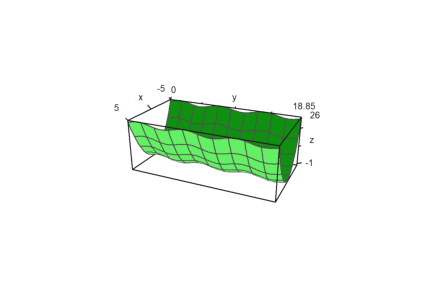
\includegraphics[width=0.5\linewidth]{EMT4Plot3D_Alifia Maylani_23030630039_MatE23-001.png}
    \caption{}
    \label{fig:enter-label}
\end{figure}

\>plot3d("x^2+x\*sin(y)",-5,5,0,6\*pi):
\begin{figure}
    \centering
    \includegraphics[width=1\linewidth]{EMT4Plot3D_Alifia Maylani_23030630039_MatE23-002.png}
    \caption{}
    \label{fig:enter-label}
\end{figure}

Silakan lakukan modifikasi agar gambar "talang bergelombang" tersebut tidak lurus melainkan melengkung/melingkar, baik
melingkar secara mendatar maupun melingkar turun/naik (seperti papan peluncur pada kolam renang. Temukan rumusnya.


# Fungsi dari dua Variabel

Untuk grafik sebuah fungsi, gunakan


* 
ekspresi sederhana dalam x dan y,

* 
nama fungsi dari dua variabell

* 
atau matriks data.


Standarnya adalah kisi-kisi kawat yang terisi dengan warna yang
berbeda di kedua sisi. Perhatikan bahwa jumlah default interval grid
adalah 10, namun plot menggunakan jumlah default 40x40 persegi panjang
untuk membangun permukaan. Hal ini dapat diubah.


* 
n=40, n=[40,40]: jumlah garis kisi di setiap arah

* 
grid=10, grid=[10,10]: jumlah garis grid di setiap arah.


Kami menggunakan default n=40 dan grid=10.


\>plot3d("x^2+y^2"):
\begin{figure}
    \centering
    \includegraphics[width=0.75\linewidth]{EMT4Plot3D_Alifia Maylani_23030630039_MatE23-003.png}
    \caption{}
    \label{fig:enter-label}
\end{figure}

Interaksi pengguna dapat dilakukan dengan parameter &gt;user. Pengguna
dapat menekan tombol berikut ini.


* 
kiri, kanan, atas, bawah: memutar sudut pandang

* 
+,-: memperbesar atau memperkecil

* 
a: menghasilkan anaglyph (lihat di bawah)

* 
l: beralih memutar sumber cahaya (lihat di bawah)

* 
spasi: mengatur ulang ke default

* 
kembali: mengakhiri interaksi


\>plot3d("exp(-x^2+y^2)",\>user, ...  
\>     title="Turn with the vector keys (press return to finish)"):


\begin{figure}
    \centering
    \includegraphics[width=0.75\linewidth]{EMT4Plot3D_Alifia Maylani_23030630039_MatE23-004.png}
    \caption{}
    \label{fig:enter-label}
\end{figure}

Rentang plot untuk fungsi dapat ditentukan dengan


* 
a, b: rentang x

* 
c, d: rentang y

* 
r: bujur sangkar simetris di sekitar (0,0).

* 
n: jumlah subinterval untuk plot.


Terdapat beberapa parameter untuk menskalakan fungsi atau mengubah
tampilan grafik.


fscale: skala untuk nilai fungsi (standarnya adalah &lt;fscale).


scale: angka atau vektor 1x2 untuk menskalakan ke arah x dan y.


frame: jenis bingkai (default 1).


\>plot3d("exp(-(x^2+y^2)/5)",r=10,n=80,fscale=4,scale=1.2,frame=3,\>user):


\begin{figure}
    \centering
    \includegraphics[width=0.75\linewidth]{EMT4Plot3D_Alifia Maylani_23030630039_MatE23-005.png}
    \caption{Enter Caption}
    \label{fig:enter-label}
\end{figure}

Tampilan dapat diubah dengan berbagai cara.


* 
jarak: jarak pandang ke plot.

* 
zoom: nilai zoom.

* 
angle: sudut ke sumbu y negatif dalam radian.

* 
height: ketinggian tampilan dalam radian.


Nilai default dapat diperiksa atau diubah dengan fungsi view(). Fungsi
ini mengembalikan parameter dalam urutan di atas.


\>view


    [5,  2.6,  2,  0.4]

Jarak yang lebih dekat membutuhkan zoom yang lebih sedikit. Efeknya
lebih seperti lensa sudut lebar.


Dalam contoh berikut ini, sudut = 0 dan tinggi = 0 terlihat dari sumbu
y negatif. Label sumbu untuk y disembunyikan dalam kasus ini.


\>plot3d("x^2+y",distance=3,zoom=1,angle=pi/2,height=0):
\begin{figure}
    \centering
    \includegraphics[width=0.75\linewidth]{EMT4Plot3D_Alifia Maylani_23030630039_MatE23-006.png}
    \caption{}
    \label{fig:enter-label}
\end{figure}
Plot terlihat selalu ke bagian tengah kubus plot. Anda dapat
memindahkan bagian tengah dengan parameter center.


\>plot3d("x^4+y^2",a=0,b=1,c=-1,d=1,angle=-20°,height=20°, ...  
\>     center=[0.4,0,0],zoom=5):


\begin{figure}
    \centering
    \includegraphics[width=0.75\linewidth]{EMT4Plot3D_Alifia Maylani_23030630039_MatE23-007.png}
    \caption{}
    \label{fig:enter-label}
\end{figure}

Plot diskalakan agar sesuai dengan kubus satuan untuk dilihat. Jadi,
tidak perlu mengubah jarak atau melakukan zoom, tergantung pada ukuran
plot. Namun demikian, label mengacu ke ukuran yang sesungguhnya.


Jika Anda menonaktifkannya dengan scale=false, Anda harus berhati-hati
agar plot tetap muat di dalam jendela plotting, dengan mengubah jarak
tampilan atau zoom, dan memindahkan bagian tengahnya.


\>plot3d("5\*exp(-x^2-y^2)",r=2,<fscale,<scale,distance=13,height=50°, ...  
\>     center=[0,0,-2],frame=3):


\begin{figure}
    \centering
    \includegraphics[width=0.75\linewidth]{EMT4Plot3D_Alifia Maylani_23030630039_MatE23-008.png}
    \caption{}
    \label{fig:enter-label}
\end{figure}
Plot polar juga tersedia. Parameter polar=true menggambar plot polar.
Fungsi harus tetap merupakan fungsi dari x dan y. Parameter “fscale”
menskalakan fungsi dengan skala sendiri. Jika tidak, fungsi akan
diskalakan agar sesuai dengan kubus.


\>plot3d("1/(x^2+y^2+1)",r=5,\>polar, ...  
\>   fscale=2,\>hue,n=100,zoom=4,\>contour,color=blue):


\begin{figure}
    \centering
    \includegraphics[width=0.75\linewidth]{EMT4Plot3D_Alifia Maylani_23030630039_MatE23-009.png}
    \caption{}
    \label{fig:enter-label}
\end{figure}

\>function f(r) := exp(-r/2)\*cos(r); ...  
\>   plot3d("f(x^2+y^2)",\>polar,scale=[1,1,0.4],r=pi,frame=3,zoom=4):


\begin{figure}
    \centering
    \includegraphics[width=0.75\linewidth]{EMT4Plot3D_Alifia Maylani_23030630039_MatE23-010.png}
    \caption{}
    \label{fig:enter-label}
\end{figure}

Parameter rotate memutar fungsi dalam x di sekitar sumbu x.


* 
rotate = 1: Menggunakan sumbu x

* 
rotate=2: Menggunakan sumbu z


\>plot3d("x^2+1",a=-1,b=1,rotate=true,grid=5):


\begin{figure}
    \centering
    \includegraphics[width=0.75\linewidth]{EMT4Plot3D_Alifia Maylani_23030630039_MatE23-011.png}
    \caption{}
    \label{fig:enter-label}
\end{figure}

\>plot3d("x^2+1",a=-1,b=1,rotate=2,grid=5):


\begin{figure}
    \centering
    \includegraphics[width=0.75\linewidth]{EMT4Plot3D_Alifia Maylani_23030630039_MatE23-012.png}
    \caption{}
    \label{fig:enter-label}
\end{figure}

\>plot3d("sqrt(25-x^2)",a=0,b=5,rotate=1):


\begin{figure}
    \centering
    \includegraphics[width=0.75\linewidth]{EMT4Plot3D_Alifia Maylani_23030630039_MatE23-013.png}
    \caption{}
    \label{fig:enter-label}
\end{figure}

\>plot3d("x\*sin(x)",a=0,b=6pi,rotate=2):


\begin{figure}
    \centering
    \includegraphics[width=0.75\linewidth]{EMT4Plot3D_Alifia Maylani_23030630039_MatE23-014.png}
    \caption{}
    \label{fig:enter-label}
\end{figure}

Berikut ini adalah plot dengan tiga fungsi.


\>plot3d("x","x^2+y^2","y",r=2,zoom=3.5,frame=3):


\begin{figure}
    \centering
    \includegraphics[width=0.75\linewidth]{EMT4Plot3D_Alifia Maylani_23030630039_MatE23-015.png}
    \caption{}
    \label{fig:enter-label}
\end{figure}
# Plot Kontur

Untuk plot, Euler menambahkan garis kisi-kisi. Sebagai gantinya,
dimungkinkan untuk menggunakan garis level dan rona satu warna atau
rona berwarna spektral. Euler dapat menggambar ketinggian fungsi pada
plot dengan bayangan. Pada semua plot 3D, Euler dapat menghasilkan
anaglyph merah/cyan.


* 
Rona: Mengaktifkan bayangan cahaya, bukan kabel.

* 
&gt;contour: Memplot garis kontur otomatis pada plot.

* 
level=... (atau level): Vektor nilai untuk garis kontur.


Defaultnya adalah level=“auto”, yang menghitung beberapa garis level
secara otomatis. Seperti yang Anda lihat di plot, level sebenarnya
adalah rentang level.


Gaya default dapat diubah. Untuk plot kontur berikut ini, kami
menggunakan grid yang lebih halus untuk 100x100 titik, skala fungsi
dan plot, dan menggunakan sudut pandang yang berbeda.


\>plot3d("exp(-x^2-y^2)",r=2,n=100,level="thin", ...  
\>    \>contour,\>spectral,fscale=1,scale=1.1,angle=45°,height=20°):


\begin{figure}
    \centering
    \includegraphics[width=0.75\linewidth]{EMT4Plot3D_Alifia Maylani_23030630039_MatE23-016.png}
    \caption{}
    \label{fig:enter-label}
\end{figure}

\>plot3d("exp(x\*y)",angle=100°,\>contour,color=green):


\begin{figure}
    \centering
    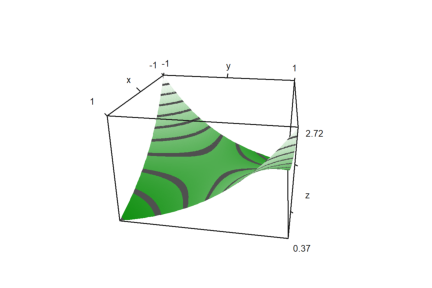
\includegraphics[width=0.75\linewidth]{EMT4Plot3D_Alifia Maylani_23030630039_MatE23-017.png}
    \caption{}
    \label{fig:enter-label}
\end{figure}

Bayangan default menggunakan warna abu-abu. Tetapi, kisaran warna
spektral juga tersedia.


* 
&gt;spektral: Menggunakan skema spektral default

* 
color =...: Menggunakan warna khusus atau skema spektral


Untuk plot berikut ini, kami menggunakan skema spektral default dan
menambah jumlah titik untuk mendapatkan tampilan yang sangat mulus.


\>plot3d("x^2+y^2",\>spectral,\>contour,n=100):


\begin{figure}
    \centering
    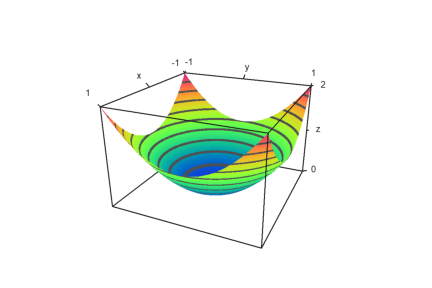
\includegraphics[width=0.75\linewidth]{EMT4Plot3D_Alifia Maylani_23030630039_MatE23-018.png}
    \caption{}
    \label{fig:enter-label}
\end{figure}

Alih-alih garis level otomatis, kita juga dapat menetapkan nilai garis
level. Hal ini akan menghasilkan garis level yang tipis, alih-alih
rentang level.


\>plot3d("x^2-y^2",0,5,0,5,level=-1:0.1:1,color=redgreen):


\begin{figure}
    \centering
    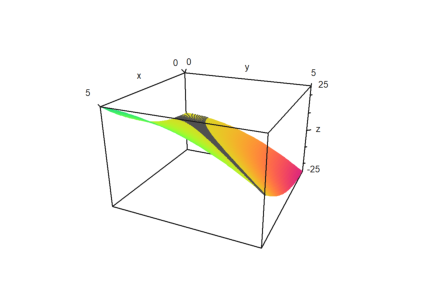
\includegraphics[width=0.75\linewidth]{EMT4Plot3D_Alifia Maylani_23030630039_MatE23-019.png}
    \caption{}
    \label{fig:enter-label}
\end{figure}

Pada plot berikut ini, kami menggunakan dua pita level yang sangat
luas dari -0,1 hingga 1, dan dari 0,9 hingga 1. Ini dimasukkan sebagai
matriks dengan batas-batas level sebagai kolom.


Selain itu, kami menghamparkan grid dengan 10 interval di setiap arah.


\>plot3d("x^2+y^3",level=[-0.1,0.9;0,1], ...  
\>     \>spectral,angle=30°,grid=10,contourcolor=gray):


\begin{figure}
    \centering
    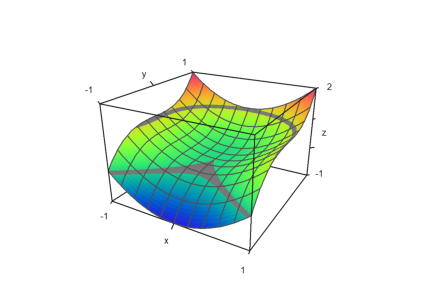
\includegraphics[width=0.75\linewidth]{EMT4Plot3D_Alifia Maylani_23030630039_MatE23-020.png}
    \caption{}
    \label{fig:enter-label}
\end{figure}

Pada contoh berikut, kami memplot himpunan, di mana


$$f(x,y) = x^y-y^x = 0$$Kita menggunakan satu garis tipis untuk garis level.


\>plot3d("x^y-y^x",level=0,a=0,b=6,c=0,d=6,contourcolor=red,n=100):


\begin{figure}
    \centering
    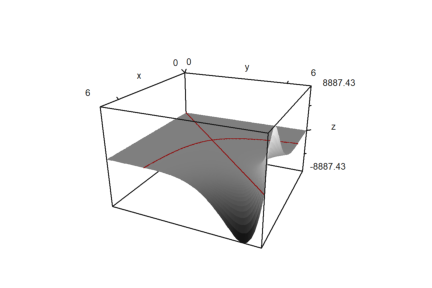
\includegraphics[width=0.75\linewidth]{EMT4Plot3D_Alifia Maylani_23030630039_MatE23-022.png}
    \caption{}
    \label{fig:enter-label}
\end{figure}

Dimungkinkan untuk menampilkan bidang kontur di bawah plot. Warna dan
jarak ke plot dapat ditentukan.


\>plot3d("x^2+y^4",\>cp,cpcolor=green,cpdelta=0.2):


\begin{figure}
    \centering
    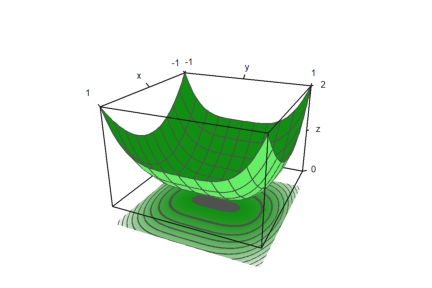
\includegraphics[width=0.75\linewidth]{EMT4Plot3D_Alifia Maylani_23030630039_MatE23-023.png}
    \caption{}
    \label{fig:enter-label}
\end{figure}

Berikut ini beberapa gaya lainnya. Kami selalu mematikan bingkai, dan
menggunakan berbagai skema warna untuk plot dan kisi-kisi.


\>figure(2,2); ...  
\>   expr="y^3-x^2"; ...  
\>   figure(1);  ...  
\>     plot3d(expr,<frame,\>cp,cpcolor=spectral); ...  
\>   figure(2);  ...  
\>     plot3d(expr,<frame,\>spectral,grid=10,cp=2); ...  
\>   figure(3);  ...  
\>     plot3d(expr,<frame,\>contour,color=gray,nc=5,cp=3,cpcolor=greenred); ...  
\>   figure(4);  ...  
\>     plot3d(expr,<frame,\>hue,grid=10,\>transparent,\>cp,cpcolor=gray); ...  
\>   figure(0):


\begin{figure}
    \centering
    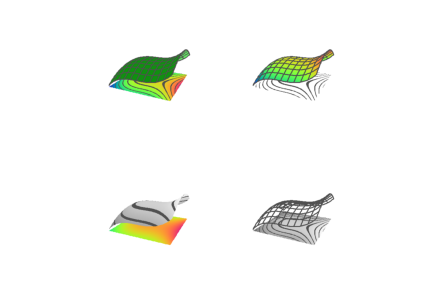
\includegraphics[width=0.75\linewidth]{EMT4Plot3D_Alifia Maylani_23030630039_MatE23-024.png}
    \caption{}
    \label{fig:enter-label}
\end{figure}

Ada beberapa skema spektral lainnya, yang diberi nomor dari 1 hingga
9. Tetapi Anda juga dapat menggunakan color=value, di mana value


* 
spektral: untuk rentang dari biru ke merah

* 
putih: untuk rentang yang lebih redup

* 
kuningbiru, ungu-hijau, biru-kuning, hijau-merah

* 
biru-kuning, hijau-ungu, kuning-biru, merah-hijau


\>figure(3,3); ...  
\>   for i=1:9;  ...  
\>     figure(i); plot3d("x^2+y^2",spectral=i,\>contour,\>cp,<frame,zoom=4);  ...  
\>   end; ...  
\>   figure(0):


\begin{figure}
    \centering
    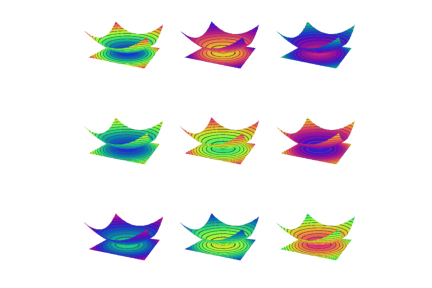
\includegraphics[width=0.75\linewidth]{EMT4Plot3D_Alifia Maylani_23030630039_MatE23-025.png}
    \caption{}
    \label{fig:enter-label}
\end{figure}

Sumber cahaya dapat diubah dengan l dan tombol kursor selama interaksi
pengguna. Ini juga dapat ditetapkan dengan parameter.


* 
light: arah cahaya

* 
amb: cahaya sekitar antara 0 dan 1


Perhatikan, bahwa program ini tidak membuat perbedaan di antara
sisi-sisi plot. Tidak ada bayangan. Untuk ini Anda akan membutuhkan
Povray.


\>plot3d("-x^2-y^2", ...  
\>     hue=true,light=[0,1,1],amb=0,user=true, ...  
\>     title="Press l and cursor keys (return to exit)"):


\begin{figure}
    \centering
    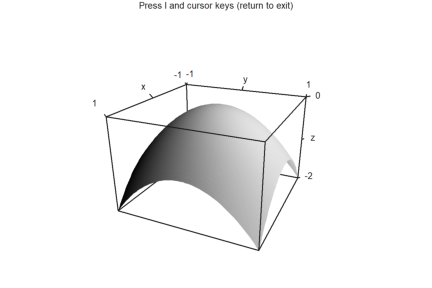
\includegraphics[width=0.75\linewidth]{EMT4Plot3D_Alifia Maylani_23030630039_MatE23-026.png}
    \caption{}
    \label{fig:enter-label}
\end{figure}

Parameter warna mengubah warna permukaan. Warna garis level juga dapat
diubah.


\>plot3d("-x^2-y^2",color=rgb(0.2,0.2,0),hue=true,frame=false, ...  
\>     zoom=3,contourcolor=red,level=-2:0.1:1,dl=0.01):


\begin{figure}
    \centering
    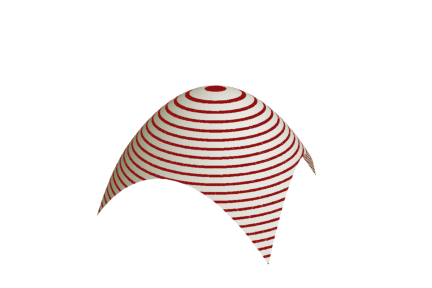
\includegraphics[width=0.75\linewidth]{EMT4Plot3D_Alifia Maylani_23030630039_MatE23-027.png}
    \caption{}
    \label{fig:enter-label}
\end{figure}

Warna 0 memberikan efek pelangi yang istimewa.


\>plot3d("x^2/(x^2+y^2+1)",color=0,hue=true,grid=10):


\begin{figure}
    \centering
    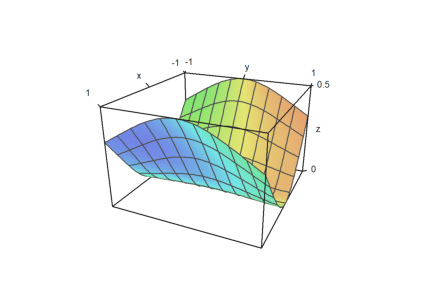
\includegraphics[width=0.75\linewidth]{EMT4Plot3D_Alifia Maylani_23030630039_MatE23-028.png}
    \caption{}
    \label{fig:enter-label}
\end{figure}

Permukaannya juga bisa transparan.


\>plot3d("x^2+y^2",\>transparent,grid=10,wirecolor=red):


\begin{figure}
    \centering
    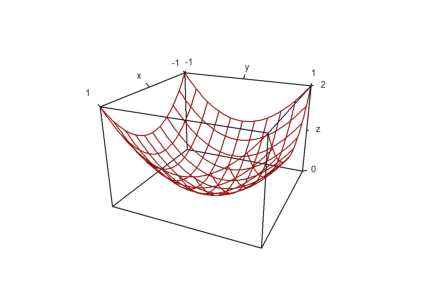
\includegraphics[width=0.75\linewidth]{EMT4Plot3D_Alifia Maylani_23030630039_MatE23-029.png}
    \caption{}
    \label{fig:enter-label}
\end{figure}

# Plot Implisit

Ada juga plot implisit dalam tiga dimensi. Euler menghasilkan potongan
melalui objek. Fitur plot3d termasuk plot implisit. Plot-plot ini
menunjukkan himpunan nol dari sebuah fungsi dalam tiga variabel.


Solusi dari


lateks: f(x,y,z) = 0


dapat divisualisasikan dalam potongan yang sejajar dengan bidang x-y,
bidang x-z, dan bidang y-z.


* 
implisit = 1: potong sejajar dengan bidang-y-z

* 
implicit = 2: memotong sejajar dengan bidang x-z

* 
implicit=4: memotong sejajar dengan bidang x-y


Tambahkan nilai-nilai ini, jika Anda mau. Pada contoh, kami memplot


$$M = \{ (x,y,z) : x^2+y^3+zy=1 \}$$\>plot3d("x^2+y^3+z\*y-1",r=5,implicit=3):


\begin{figure}
    \centering
    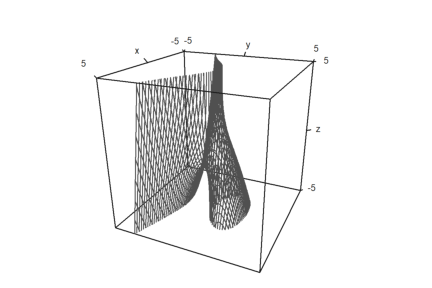
\includegraphics[width=0.75\linewidth]{EMT4Plot3D_Alifia Maylani_23030630039_MatE23-031.png}
    \caption{}
    \label{fig:enter-label}
\end{figure}

\>c=1; d=1;

\>plot3d("((x^2+y^2-c^2)^2+(z^2-1)^2)\*((y^2+z^2-c^2)^2+(x^2-1)^2)\*((z^2+x^2-c^2)^2+(y^2-1)^2)-d",r=2,<frame,\>implicit,\>user): 


\begin{figure}
    \centering
    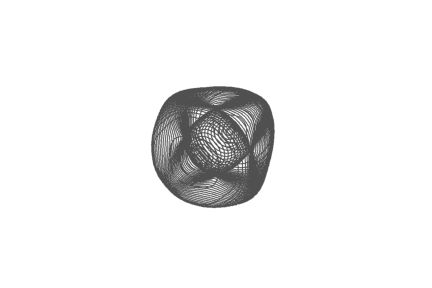
\includegraphics[width=0.75\linewidth]{EMT4Plot3D_Alifia Maylani_23030630039_MatE23-032.png}
    \caption{}
    \label{fig:enter-label}
\end{figure}

\>plot3d("x^2+y^2+4\*x\*z+z^3",\>implicit,r=2,zoom=2.5):


\begin{figure}
    \centering
    \includegraphics[width=0.75\linewidth]{EMT4Plot3D_Alifia Maylani_23030630039_MatE23-033.png}
    \caption{}
    \label{fig:enter-label}
\end{figure}

# Memplot Data 3D

Sama seperti plot2d, plot3d menerima data. Untuk objek 3D, Anda perlu
menyediakan matriks nilai x, y, dan z, atau tiga fungsi atau ekspresi
fx(x,y), fy(x,y), fz(x,y).


$$\gamma(t,s) = (x(t,s),y(t,s),z(t,s))$$arena x,y,z adalah matriks, kita mengasumsikan bahwa (t,s) berjalan
melalui kotak persegi. Hasilnya, Anda dapat memplot gambar persegi
panjang dalam ruang.


Anda dapat menggunakan bahasa matriks Euler untuk menghasilkan
koordinat secara efektif.


Pada contoh berikut, kita menggunakan vektor nilai t dan vektor kolom
nilai s untuk memparameterkan permukaan bola. Pada gambar kita dapat
menandai daerah, dalam kasus kita daerah kutub.


\>t=linspace(0,2pi,180); s=linspace(-pi/2,pi/2,90)'; ...  
\>   x=cos(s)\*cos(t); y=cos(s)\*sin(t); z=sin(s); ...  
\>   plot3d(x,y,z,\>hue, ...  
\>   color=blue,<frame,grid=[10,20], ...  
\>   values=s,contourcolor=red,level=[90°-24°;90°-22°], ...  
\>   scale=1.4,height=50°):


\begin{figure}
    \centering
    \includegraphics[width=0.75\linewidth]{EMT4Plot3D_Alifia Maylani_23030630039_MatE23-035.png}
    \caption{}
    \label{fig:enter-label}
\end{figure}

Berikut ini adalah contoh, yang merupakan grafik suatu fungsi.


\>t=-1:0.1:1; s=(-1:0.1:1)'; plot3d(t,s,t\*s,grid=10):


\begin{figure}
    \centering
    \includegraphics[width=0.75\linewidth]{EMT4Plot3D_Alifia Maylani_23030630039_MatE23-036.png}
    \caption{}
    \label{fig:enter-label}
\end{figure}

Namun demikian, kita bisa membuat segala macam permukaan. Berikut ini
adalah permukaan yang sama dengan fungsi


$$x = y \, z$$\>plot3d(t\*s,t,s,angle=180°,grid=10):


\begin{figure}
    \centering
    \includegraphics[width=0.75\linewidth]{EMT4Plot3D_Alifia Maylani_23030630039_MatE23-038.png}
    \caption{}
    \label{fig:enter-label}
\end{figure}

Dengan lebih banyak upaya, kita bisa menghasilkan banyak permukaan.


Dalam contoh berikut ini, kami membuat tampilan berbayang dari bola
yang terdistorsi. Koordinat biasa untuk bola adalah


$$\gamma(t,s) = (\cos(t)\cos(s),\sin(t)\sin(s),\cos(s))$$dengan


$$0 \le t \le 2\pi, \quad \frac{-\pi}{2} \le s \le \frac{\pi}{2}.$$Kami mengurangi hal ini dengan faktor


$$d(t,s) = \frac{\cos(4t)+\cos(8s)}{4}.$$\>t=linspace(0,2pi,320); s=linspace(-pi/2,pi/2,160)'; ...  
\>   d=1+0.2\*(cos(4\*t)+cos(8\*s)); ...  
\>   plot3d(cos(t)\*cos(s)\*d,sin(t)\*cos(s)\*d,sin(s)\*d,hue=1, ...  
\>     light=[1,0,1],frame=0,zoom=5):


\begin{figure}
    \centering
    \includegraphics[width=0.75\linewidth]{EMT4Plot3D_Alifia Maylani_23030630039_MatE23-042.png}
    \caption{}
    \label{fig:enter-label}
\end{figure}

Tentu saja, awan titik juga dimungkinkan. Untuk memplot data titik
dalam ruang, kita membutuhkan tiga vektor untuk koordinat titik.


Gaya-gayanya sama seperti pada plot2d dengan points=true;


\>n=500;  ...  
\>     plot3d(normal(1,n),normal(1,n),normal(1,n),points=true,style="."):


\begin{figure}
    \centering
    \includegraphics[width=0.75\linewidth]{EMT4Plot3D_Alifia Maylani_23030630039_MatE23-043.png}
    \caption{}
    \label{fig:enter-label}
\end{figure}

Anda juga dapat memplot kurva dalam bentuk 3D. Dalam hal ini, akan
lebih mudah untuk menghitung titik-titik kurva. Untuk kurva pada
bidang, kami menggunakan urutan koordinat dan parameter wire = true.


\>t=linspace(0,8pi,500); ...  
\>   plot3d(sin(t),cos(t),t/10,\>wire,zoom=3):


\begin{figure}
    \centering
    \includegraphics[width=0.75\linewidth]{EMT4Plot3D_Alifia Maylani_23030630039_MatE23-044.png}
    \caption{}
    \label{fig:enter-label}
\end{figure}

\>t=linspace(0,4pi,1000); plot3d(cos(t),sin(t),t/2pi,\>wire, ...  
\>   linewidth=3,wirecolor=blue):


\begin{figure}
    \centering
    \includegraphics[width=0.75\linewidth]{EMT4Plot3D_Alifia Maylani_23030630039_MatE23-045.png}
    \caption{}
    \label{fig:enter-label}
\end{figure}

\>X=cumsum(normal(3,100)); ...  
\>    plot3d(X[1],X[2],X[3],\>anaglyph,\>wire):


\begin{figure}
    \centering
    \includegraphics[width=0.75\linewidth]{EMT4Plot3D_Alifia Maylani_23030630039_MatE23-046.png}
    \caption{}
    \label{fig:enter-label}
\end{figure}

EMT juga dapat membuat plot dalam mode anaglyph. Untuk melihat plot
semacam itu, Anda memerlukan kacamata merah/cyan.


\> plot3d("x^2+y^3",\>anaglyph,\>contour,angle=30°):


\begin{figure}
    \centering
    \includegraphics[width=0.75\linewidth]{EMT4Plot3D_Alifia Maylani_23030630039_MatE23-047.png}
    \caption{}
    \label{fig:enter-label}
\end{figure}

Sering kali, skema warna spektral digunakan untuk plot. Hal ini
menekankan ketinggian fungsi.


\> plot3d("x^2\*y^3-y",\>spectral,\>contour,zoom=3.2):


\begin{figure}
    \centering
    \includegraphics[width=0.75\linewidth]{EMT4Plot3D_Alifia Maylani_23030630039_MatE23-048.png}
    \caption{}
    \label{fig:enter-label}
\end{figure}

Euler juga dapat memplot permukaan yang diparameterkan, ketika
parameternya adalah nilai x-, y-, dan z- dari gambar kisi-kisi persegi
panjang di dalam ruang.


Untuk demo berikut ini, kami menyiapkan parameter u- dan v-, dan
menghasilkan koordinat ruang dari parameter ini.


\>u=linspace(-1,1,10); v=linspace(0,2\*pi,50)'; ...  
\>   X=(3+u\*cos(v/2))\*cos(v); Y=(3+u\*cos(v/2))\*sin(v); Z=u\*sin(v/2); ...  
\>   plot3d(X,Y,Z,\>anaglyph,<frame,\>wire,scale=2.3):


\begin{figure}
    \centering
    \includegraphics[width=0.75\linewidth]{EMT4Plot3D_Alifia Maylani_23030630039_MatE23-049.png}
    \caption{}
    \label{fig:enter-label}
\end{figure}

Berikut ini contoh yang lebih rumit, yang tampak megah dengan kacamata
merah/cyan.


\>u:=linspace(-pi,pi,160); v:=linspace(-pi,pi,400)';  ...  
\>   x:=(4\*(1+.25\*sin(3\*v))+cos(u))\*cos(2\*v); ...  
\>   y:=(4\*(1+.25\*sin(3\*v))+cos(u))\*sin(2\*v); ...  
\>    z=sin(u)+2\*cos(3\*v); ...  
\>   plot3d(x,y,z,frame=0,scale=1.5,hue=1,light=[1,0,-1],zoom=2.8,\>anaglyph):


\begin{figure}
    \centering
    \includegraphics[width=0.75\linewidth]{EMT4Plot3D_Alifia Maylani_23030630039_MatE23-050.png}
    \caption{}
    \label{fig:enter-label}
\end{figure}

# Plot Statistik

Plot batang juga dapat digunakan. Untuk ini, kita harus menyediakan


* 
x: vektor baris dengan n+1 elemen

* 
y: vektor kolom dengan n+1 elemen

* 
z: matriks nilai berukuran nxn.


z dapat lebih besar, tetapi hanya nilai nxn yang akan digunakan.


Pada contoh, pertama-tama kita menghitung nilainya. Kemudian kita
sesuaikan x dan y, sehingga vektor berada di tengah-tengah nilai yang
digunakan.


\>x=-1:0.1:1; y=x'; z=x^2+y^2; ...  
\>   xa=(x|1.1)-0.05; ya=(y\_1.1)-0.05; ...  
\>   plot3d(xa,ya,z,bar=true):


\begin{figure}
    \centering
    \includegraphics[width=0.75\linewidth]{EMT4Plot3D_Alifia Maylani_23030630039_MatE23-051.png}
    \caption{}
    \label{fig:enter-label}
\end{figure}

Dimungkinkan untuk membagi plot permukaan menjadi dua bagian atau
lebih.


\>x=-1:0.1:1; y=x'; z=x+y; d=zeros(size(x)); ...  
\>   plot3d(x,y,z,disconnect=2:2:20):


\begin{figure}
    \centering
    \includegraphics[width=0.75\linewidth]{EMT4Plot3D_Alifia Maylani_23030630039_MatE23-052.png}
    \caption{}
    \label{fig:enter-label}
\end{figure}

Jika memuat atau menghasilkan matriks data M dari file dan perlu
memplotnya dalam 3D, Anda dapat menskalakan matriks ke [-1,1] dengan
scale(M), atau menskalakan matriks dengan &gt;zscale. Hal ini dapat
dikombinasikan dengan faktor penskalaan individual yang diterapkan
sebagai tambahan.


\>i=1:20; j=i'; ...  
\>   plot3d(i\*j^2+100\*normal(20,20),\>zscale,scale=[1,1,1.5],angle=-40°,zoom=1.8):


\begin{figure}
    \centering
    \includegraphics[width=0.75\linewidth]{EMT4Plot3D_Alifia Maylani_23030630039_MatE23-053.png}
    \caption{}
    \label{fig:enter-label}
\end{figure}

\>Z=intrandom(5,100,6); v=zeros(5,6); ...  
\>   loop 1 to 5; v[#]=getmultiplicities(1:6,Z[#]); end; ...  
\>   columnsplot3d(v',scols=1:5,ccols=[1:5]):


\begin{figure}
    \centering
    \includegraphics[width=0.75\linewidth]{EMT4Plot3D_Alifia Maylani_23030630039_MatE23-054.png}
    \caption{}
    \label{fig:enter-label}
\end{figure}

# Permukaan Benda Putar

\>plot2d("(x^2+y^2-1)^3-x^2\*y^3",r=1.3, ...  
\>   style="#",color=red,<outline, ...  
\>   level=[-2;0],n=100):


\begin{figure}
    \centering
    \includegraphics[width=0.75\linewidth]{EMT4Plot3D_Alifia Maylani_23030630039_MatE23-055.png}
    \caption{}
    \label{fig:enter-label}
\end{figure}

\>ekspresi &= (x^2+y^2-1)^3-x^2\*y^3; $ekspresi


$$\left(y^2+x^2-1\right)^3-x^2\,y^3$$Kami ingin memutar kurva jantung di sekitar sumbu y. Inilah ekspresi
yang mendefinisikan jantung:


$$f(x,y)=(x^2+y^2-1)^3-x^2.y^3.$$Selanjutnya kami menetapkan


$$x=r.cos(a),\quad y=r.sin(a).$$\>function fr(r,a) &= ekspresi with [x=r\*cos(a),y=r\*sin(a)] | trigreduce; $fr(r,a)


$$\left(r^2-1\right)^3+\frac{\left(\sin \left(5\,a\right)-\sin \left(
 3\,a\right)-2\,\sin a\right)\,r^5}{16}$$Hal ini memungkinkan untuk mendefinisikan fungsi numerik, yang
menyelesaikan untuk r, jika a diberikan. Dengan fungsi tersebut kita
dapat memplotkan jantung yang diputar sebagai permukaan parametrik.


\>function map f(a) := bisect("fr",0,2;a); ...  
\>   t=linspace(-pi/2,pi/2,100); r=f(t);  ...  
\>   s=linspace(pi,2pi,100)'; ...  
\>   plot3d(r\*cos(t)\*sin(s),r\*cos(t)\*cos(s),r\*sin(t), ...  
\>   \>hue,<frame,color=red,zoom=4,amb=0,max=0.7,grid=12,height=50°):


\begin{figure}
    \centering
    \includegraphics[width=0.75\linewidth]{EMT4Plot3D_Alifia Maylani_23030630039_MatE23-060.png}
    \caption{}
    \label{fig:enter-label}
\end{figure}

Berikut ini adalah plot 3D dari gambar di atas yang diputar
mengelilingi sumbu-z. Kami mendefinisikan fungsi, yang menggambarkan
objek.


\>function f(x,y,z) ...


    r=x^2+y^2;
    return (r+z^2-1)^3-r*z^3;
     endfunction
</pre>
\>plot3d("f(x,y,z)", ...  
\>   xmin=0,xmax=1.2,ymin=-1.2,ymax=1.2,zmin=-1.2,zmax=1.4, ...  
\>   implicit=1,angle=-30°,zoom=2.5,n=[10,100,60],\>anaglyph):


\begin{figure}
    \centering
    \includegraphics[width=0.75\linewidth]{EMT4Plot3D_Alifia Maylani_23030630039_MatE23-061.png}
    \caption{}
    \label{fig:enter-label}
\end{figure}

# Plot 3D Khusus

Fungsi plot3d memang bagus untuk dimiliki, tetapi tidak memenuhi semua
kebutuhan. Selain rutinitas yang lebih mendasar, Anda juga bisa
mendapatkan plot berbingkai dari objek apa pun yang Anda sukai.


Meskipun Euler bukan program 3D, namun dapat menggabungkan beberapa
objek dasar. Kami mencoba memvisualisasikan parabola dan garis
singgungnya.


\>function myplot ...


      y=-1:0.01:1; x=(-1:0.01:1)';
      plot3d(x,y,0.2*(x-0.1)/2,<scale,<frame,>hue, ..
        hues=0.5,>contour,color=orange);
      h=holding(1);
      plot3d(x,y,(x^2+y^2)/2,<scale,<frame,>contour,>hue);
      holding(h);
    endfunction
</pre>
Sekarang framedplot() menyediakan frame, dan mengatur tampilan.


\>framedplot("myplot",[-1,1,-1,1,0,1],height=0,angle=-30°, ...  
\>     center=[0,0,-0.7],zoom=3):


\begin{figure}
    \centering
    \includegraphics[width=0.75\linewidth]{EMT4Plot3D_Alifia Maylani_23030630039_MatE23-062.png}
    \caption{}
    \label{fig:enter-label}
\end{figure}

Dengan cara yang sama, Anda dapat memplot bidang kontur secara manual.
Perhatikan bahwa plot3d() mengatur jendela ke fullwindow() secara
default, namun plotcontourplane() mengasumsikannya.


\>x=-1:0.02:1.1; y=x'; z=x^2-y^4;

\>function myplot (x,y,z) ...  
\>  
<pre class="udf">      zoom(2);
      wi=fullwindow();
      plotcontourplane(x,y,z,level="auto",<scale);
      plot3d(x,y,z,>hue,<scale,>add,color=white,level="thin");
      window(wi);
      reset();
    endfunction
</pre>
\>myplot(x,y,z):


\begin{figure}
    \centering
    \includegraphics[width=0.75\linewidth]{EMT4Plot3D_Alifia Maylani_23030630039_MatE23-063.png}
    \caption{}
    \label{fig:enter-label}
\end{figure}

# Animasi

Euler dapat menggunakan frame untuk melakukan pra-komputasi animasi.


Salah satu fungsi yang memanfaatkan teknik ini adalah rotate. Fungsi
ini dapat mengubah sudut pandang dan menggambar ulang plot 3D. Fungsi
ini memanggil addpage() untuk setiap plot baru. Akhirnya fungsi ini
menganimasikan plot tersebut.


Silakan pelajari sumber dari rotate untuk melihat lebih detail.


\>function testplot () := plot3d("x^2+y^3"); ...  
\>   rotate("testplot"); testplot():


\begin{figure}
    \centering
    \includegraphics[width=0.75\linewidth]{EMT4Plot3D_Alifia Maylani_23030630039_MatE23-064.png}
    \caption{}
    \label{fig:enter-label}
\end{figure}

# Menggambar Povray

Dengan bantuan file Euler povray.e, Euler dapat menghasilkan file
Povray. Hasilnya sangat bagus untuk dilihat.


Anda perlu menginstal Povray (32bit atau 64bit) dari
  <a href="http://www.povray.org/, dan meletakkan sub-direktori “bin” dari Povray ke dalam jalur lingkungan, atau mengatur variabel “defaultpovray” dengan jalur lengkap yang mengarah ke “pvengine.exe”.">http://www.povray.org/, dan meletakkan sub-direktori “bin” dari Povray ke dalam jalur lingkungan, atau mengatur variabel “defaultpovray” dengan jalur lengkap yang mengarah ke “pvengine.exe”.</a>


Antarmuka Povray dari Euler menghasilkan file Povray di direktori home
pengguna, dan memanggil Povray untuk mengurai file-file ini. Nama file
default adalah current.pov, dan direktori defaultnya adalah
eulerhome(), biasanya c:\Users\Username\Euler. Povray menghasilkan
sebuah file PNG, yang dapat dimuat oleh Euler ke dalam notebook. Untuk
membersihkan berkas-berkas ini, gunakan povclear().


Fungsi pov3d memiliki semangat yang sama dengan plot3d. Fungsi ini
dapat menghasilkan grafik dari sebuah fungsi f(x,y), atau sebuah
permukaan dengan koordinat X,Y,Z dalam bentuk matriks, termasuk
garis-garis level yang bersifat opsional. Fungsi ini memulai raytracer
secara otomatis, dan memuat adegan ke dalam notebook Euler.


Selain pov3d(), ada banyak fungsi yang menghasilkan objek Povray.
Fungsi-fungsi ini mengembalikan string, yang berisi kode Povray untuk
objek. Untuk menggunakan fungsi-fungsi ini, mulai file Povray dengan
povstart(). Kemudian gunakan writeln(...) untuk menulis objek ke file
scene. Terakhir, akhiri file dengan povend(). Secara default,
raytracer akan dimulai, dan PNG akan dimasukkan ke dalam buku catatan
Euler.


Fungsi objek memiliki parameter yang disebut “look”, yang membutuhkan
string dengan kode povray untuk tekstur dan hasil akhir objek. Fungsi
povlook() dapat digunakan untuk menghasilkan string ini. Fungsi ini
memiliki parameter untuk warna, transparansi, Phong Shading, dll.


Perhatikan bahwa Povray universe memiliki sistem koordinat lain.
Antarmuka ini menerjemahkan semua koordinat ke sistem Povray. Jadi
Anda dapat tetap berpikir dalam sistem koordinat Euler dengan z yang
mengarah vertikal ke atas, dan sumbu x, y, z di tangan kanan.


Anda perlu memuat file povray.


\>load povray;


Pastikan direktori bin povray berada di dalam path. Jika tidak, edit
variabel berikut sehingga berisi jalur ke povray yang dapat
dieksekusi.


\>defaultpovray="C:\\Program Files\\POV-Ray\\v3.7\\bin\\pvengine.exe"


    C:\Program Files\POV-Ray\v3.7\bin\pvengine.exe

Untuk kesan pertama, kita plot sebuah fungsi sederhana. Perintah
berikut ini menghasilkan file povray di direktori pengguna Anda, dan
menjalankan Povray untuk melacak sinar pada file ini.


Jika Anda memulai perintah berikut, GUI Povray akan terbuka,
menjalankan file, dan menutup secara otomatis. Karena alasan keamanan,
Anda akan ditanya, apakah Anda ingin mengizinkan file exe dijalankan.
Anda dapat menekan cancel untuk menghentikan pertanyaan lebih lanjut.
Anda mungkin harus menekan OK pada jendela Povray untuk mengetahui
dialog awal Povray.


\>plot3d("x^2+y^2",zoom=2):


\begin{figure}
    \centering
    \includegraphics[width=0.75\linewidth]{EMT4Plot3D_Alifia Maylani_23030630039_MatE23-065.png}
    \caption{}
    \label{fig:enter-label}
\end{figure}

\>pov3d("x^2+y^2",zoom=3);


![images/EMT4Plot3D_Alifia%20Maylani_23030630039_MatE23-066.png](images/EMT4Plot3D_Alifia%20Maylani_23030630039_MatE23-066.png)

Kita dapat membuat fungsi menjadi transparan dan menambahkan hasil
akhir lainnya. Kita juga dapat menambahkan garis level ke plot fungsi.


\>pov3d("x^2+y^3",axiscolor=red,angle=-45°,\>anaglyph, ...  
\>     look=povlook(cyan,0.2),level=-1:0.5:1,zoom=3.8);




\begin{figure}
    \centering
    \includegraphics[width=0.5\linewidth]{EMT4Plot3D_Alifia Maylani_23030630039_MatE23-066.png}
    \caption{}
    \label{fig:enter-label}
\end{figure}

\begin{figure}
    \centering
    \includegraphics[width=0.75\linewidth]{EMT4Plot3D_Alifia Maylani_23030630039_MatE23-067.png}
    \caption{}
    \label{fig:enter-label}
\end{figure}

Kadang-kadang perlu untuk mencegah penskalaan fungsi, dan menskalakan
fungsi dengan tangan.


Kami memplot kumpulan titik pada bidang kompleks, di mana hasil kali
jarak ke 1 dan -1 sama dengan 1.


\>pov3d("((x-1)^2+y^2)\*((x+1)^2+y^2)/40",r=2, ...  
\>     angle=-120°,level=1/40,dlevel=0.005,light=[-1,1,1],height=10°,n=50, ...  
\>     <fscale,zoom=3.8);


\begin{figure}
    \centering
    \includegraphics[width=0.75\linewidth]{EMT4Plot3D_Alifia Maylani_23030630039_MatE23-068.png}
    \caption{}
    \label{fig:enter-label}
\end{figure}

# Merencanakan dengan Koordinat

Sebagai pengganti fungsi, kita dapat membuat plot dengan koordinat.
Seperti pada plot3d, kita membutuhkan tiga matriks untuk
mendefinisikan objek.


Pada contoh, kita memutar sebuah fungsi pada sumbu z.


\>function f(x) := x^3-x+1; ...  
\>   x=-1:0.01:1; t=linspace(0,2pi,50)'; ...  
\>   Z=x; X=cos(t)\*f(x); Y=sin(t)\*f(x); ...  
\>   pov3d(X,Y,Z,angle=40°,look=povlook(red,0.1),height=50°,axis=0,zoom=4,light=[10,5,15]);


\begin{figure}
    \centering
    \includegraphics[width=0.75\linewidth]{EMT4Plot3D_Alifia Maylani_23030630039_MatE23-069.png}
    \caption{}
    \label{fig:enter-label}
\end{figure}

Pada contoh berikut, kita memplot gelombang teredam. Kami menghasilkan
gelombang dengan bahasa matriks Euler.


Kami juga menunjukkan, bagaimana objek tambahan dapat ditambahkan ke
adegan pov3d. Untuk pembuatan objek, lihat contoh berikut. Perhatikan
bahwa plot3d menskalakan plot, sehingga sesuai dengan kubus satuan.


\>r=linspace(0,1,80); phi=linspace(0,2pi,80)'; ...  
\>   x=r\*cos(phi); y=r\*sin(phi); z=exp(-5\*r)\*cos(8\*pi\*r)/3;  ...  
\>   pov3d(x,y,z,zoom=6,axis=0,height=30°,add=povsphere([0.5,0,0.25],0.15,povlook(red)), ...  
\>     w=500,h=300);


\begin{figure}
    \centering
    \includegraphics[width=0.75\linewidth]{EMT4Plot3D_Alifia Maylani_23030630039_MatE23-070.png}
    \caption{}
    \label{fig:enter-label}
\end{figure}

Dengan metode bayangan canggih Povray, hanya sedikit titik yang bisa
menghasilkan permukaan yang sangat halus. Hanya pada batas-batas dan
bayangan, trik ini bisa terlihat jelas.


Untuk itu, kita perlu menambahkan vektor normal di setiap titik
matriks.


\>Z &= x^2\*y^3


    
                                     2  3
                                    x  y
    

Persamaan permukaannya adalah [x,y,Z]. Kami menghitung dua turunan
terhadap x dan y dari persamaan ini dan mengambil hasil perkalian
silang sebagai normal.


\>dx &= diff([x,y,Z],x); dy &= diff([x,y,Z],y);


Kami mendefinisikan normal sebagai hasil kali silang dari turunan ini,
dan mendefinisikan fungsi koordinat.


\>N &= crossproduct(dx,dy); NX &= N[1]; NY &= N[2]; NZ &= N[3]; N,


    
                                   3       2  2
                           [- 2 x y , - 3 x  y , 1]
    

Kami hanya menggunakan 25 poin.


\>x=-1:0.5:1; y=x';

\>pov3d(x,y,Z(x,y),angle=10°, ...  
\>     xv=NX(x,y),yv=NY(x,y),zv=NZ(x,y),<shadow);


\begin{figure}
    \centering
    \includegraphics[width=0.75\linewidth]{EMT4Plot3D_Alifia Maylani_23030630039_MatE23-071.png}
    \caption{}
    \label{fig:enter-label}
\end{figure}

Berikut ini adalah simpul Trefoil yang dibuat oleh A. Busser di
Povray. Ada versi yang lebih baik dari ini dalam contoh.


  <a href="Examples\Trefoil Knot.html">Trefoil Knot</a>  

Untuk tampilan yang bagus dengan tidak terlalu banyak titik, kami
menambahkan vektor normal di sini. Kami menggunakan Maxima untuk
menghitung normal untuk kami. Pertama, tiga fungsi untuk koordinat
sebagai ekspresi simbolis.


\>X &= ((4+sin(3\*y))+cos(x))\*cos(2\*y); ...  
\>   Y &= ((4+sin(3\*y))+cos(x))\*sin(2\*y); ...  
\>   Z &= sin(x)+2\*cos(3\*y);


Kemudian dua vektor turunan terhadap x dan y.


\>dx &= diff([X,Y,Z],x); dy &= diff([X,Y,Z],y);


Sekarang yang normal, yang merupakan produk silang dari dua turunan.


\>dn &= crossproduct(dx,dy);


Kami sekarang mengevaluasi semua ini secara numerik.


\>x:=linspace(-%pi,%pi,40); y:=linspace(-%pi,%pi,100)';


Vektor normal adalah evaluasi dari ekspresi simbolik dn[i] untuk
i=1,2,3. Sintaks untuk ini adalah &amp;“ekspresi”(parameter). Ini adalah
sebuah alternatif dari metode pada contoh sebelumnya, di mana kita
mendefinisikan ekspresi simbolik NX, NY, NZ terlebih dahulu.


\>pov3d(X(x,y),Y(x,y),Z(x,y),\>anaglyph,axis=0,zoom=5,w=450,h=350, ...  
\>     <shadow,look=povlook(blue), ...  
\>     xv=&"dn[1]"(x,y), yv=&"dn[2]"(x,y), zv=&"dn[3]"(x,y));


\begin{figure}
    \centering
    \includegraphics[width=0.75\linewidth]{EMT4Plot3D_Alifia Maylani_23030630039_MatE23-072.png}
    \caption{}
    \label{fig:enter-label}
\end{figure}

Kami juga dapat menghasilkan kisi-kisi dalam bentuk 3D.


\>povstart(zoom=4); ...  
\>   x=-1:0.5:1; r=1-(x+1)^2/6; ...  
\>   t=(0°:30°:360°)'; y=r\*cos(t); z=r\*sin(t); ...  
\>   writeln(povgrid(x,y,z,d=0.02,dballs=0.05)); ...  
\>   povend();


\begin{figure}
    \centering
    \includegraphics[width=0.75\linewidth]{EMT4Plot3D_Alifia Maylani_23030630039_MatE23-073.png}
    \caption{}
    \label{fig:enter-label}
\end{figure}

Dengan povgrid(), kurva dapat dibuat.


\>povstart(center=[0,0,1],zoom=3.6); ...  
\>   t=linspace(0,2,1000); r=exp(-t); ...  
\>   x=cos(2\*pi\*10\*t)\*r; y=sin(2\*pi\*10\*t)\*r; z=t; ...  
\>   writeln(povgrid(x,y,z,povlook(red))); ...  
\>   writeAxis(0,2,axis=3); ...  
\>   povend();


\begin{figure}
    \centering
    \includegraphics[width=0.75\linewidth]{EMT4Plot3D_Alifia Maylani_23030630039_MatE23-074.png}
    \caption{}
    \label{fig:enter-label}
\end{figure}

# Objek Povray

Di atas, kami menggunakan pov3d untuk memplot permukaan. Antarmuka
povray di Euler juga dapat menghasilkan objek Povray. Objek-objek ini
disimpan sebagai string di Euler, dan perlu ditulis ke file Povray.


Kita memulai output dengan povstart().


\>povstart(zoom=4);


Pertama, kita mendefinisikan tiga silinder, dan menyimpannya dalam
bentuk string di Euler.


Fungsi povx() dll. hanya mengembalikan vektor [1,0,0], yang dapat
digunakan sebagai gantinya.


\>c1=povcylinder(-povx,povx,1,povlook(red)); ...  
\>   c2=povcylinder(-povy,povy,1,povlook(yellow)); ...  
\>   c3=povcylinder(-povz,povz,1,povlook(blue)); ...  
\>  
The strings contain Povray code, which we need not understand at that
point.


\>c2


    cylinder { &lt;0,0,-1&gt;, &lt;0,0,1&gt;, 1
     texture { pigment { color rgb &lt;0.941176,0.941176,0.392157&gt; }  } 
     finish { ambient 0.2 } 
     }

Seperti yang Anda lihat, kami menambahkan tekstur ke objek dalam tiga
warna berbeda.


Hal ini dilakukan dengan povlook(), yang mengembalikan sebuah string
dengan kode Povray yang relevan. Kita dapat menggunakan warna default
Euler, atau menentukan warna kita sendiri. Kita juga dapat menambahkan
transparansi, atau mengubah cahaya sekitar.


\>povlook(rgb(0.1,0.2,0.3),0.1,0.5)


     texture { pigment { color rgbf &lt;0.101961,0.2,0.301961,0.1&gt; }  } 
     finish { ambient 0.5 } 
    

Sekarang kita mendefinisikan objek perpotongan, dan menulis hasilnya
ke file.


\>writeln(povintersection([c1,c2,c3]));


Perpotongan tiga silinder sulit untuk divisualisasikan, jika Anda
belum pernah melihatnya.


\>povend;


\begin{figure}
    \centering
    \includegraphics[width=0.75\linewidth]{EMT4Plot3D_Alifia Maylani_23030630039_MatE23-075.png}
    \caption{}
    \label{fig:enter-label}
\end{figure}

Fungsi-fungsi berikut ini menghasilkan fraktal secara rekursif.


Fungsi pertama menunjukkan, bagaimana Euler menangani objek Povray
sederhana. Fungsi povbox() mengembalikan sebuah string, yang berisi
koordinat kotak, tekstur dan hasil akhir.


\>function onebox(x,y,z,d) := povbox([x,y,z],[x+d,y+d,z+d],povlook());

\>function fractal (x,y,z,h,n) ...  
\>  
<pre class="udf">     if n==1 then writeln(onebox(x,y,z,h));
     else
       h=h/3;
       fractal(x,y,z,h,n-1);
       fractal(x+2*h,y,z,h,n-1);
       fractal(x,y+2*h,z,h,n-1);
       fractal(x,y,z+2*h,h,n-1);
       fractal(x+2*h,y+2*h,z,h,n-1);
       fractal(x+2*h,y,z+2*h,h,n-1);
       fractal(x,y+2*h,z+2*h,h,n-1);
       fractal(x+2*h,y+2*h,z+2*h,h,n-1);
       fractal(x+h,y+h,z+h,h,n-1);
     endif;
    endfunction
</pre>
\>povstart(fade=10,<shadow);

\>fractal(-1,-1,-1,2,4);

\>povend();


\begin{figure}
    \centering
    \includegraphics[width=0.75\linewidth]{EMT4Plot3D_Alifia Maylani_23030630039_MatE23-076.png}
    \caption{}
    \label{fig:enter-label}
\end{figure}

Perbedaan memungkinkan pemotongan satu objek dari objek lainnya.
Seperti persimpangan, ada bagian dari objek CSG Povray.


\>povstart(light=[5,-5,5],fade=10);


Untuk demonstrasi ini, kita mendefinisikan sebuah objek di Povray,
alih-alih menggunakan string di Euler. Definisi akan langsung
dituliskan ke file.


Koordinat kotak -1 berarti [-1,-1,-1].


\>povdefine("mycube",povbox(-1,1));


Kita dapat menggunakan objek ini dalam povobject(), yang mengembalikan
sebuah string seperti biasa.


\>c1=povobject("mycube",povlook(red));


Kami menghasilkan kubus kedua, dan memutar serta menskalakannya
sedikit.


\>c2=povobject("mycube",povlook(yellow),translate=[1,1,1], ...  
\>     rotate=xrotate(10°)+yrotate(10°), scale=1.2);


Kemudian kita ambil selisih dari kedua objek tersebut.


\>writeln(povdifference(c1,c2));


Sekarang tambahkan tiga sumbu.


\>writeAxis(-1.2,1.2,axis=1); ...  
\>   writeAxis(-1.2,1.2,axis=2); ...  
\>   writeAxis(-1.2,1.2,axis=4); ...  
\>   povend();


\begin{figure}
    \centering
    \includegraphics[width=0.75\linewidth]{EMT4Plot3D_Alifia Maylani_23030630039_MatE23-077.png}
    \caption{}
    \label{fig:enter-label}
\end{figure}

# Fungsi Implisit

Povray dapat memplot himpunan di mana f(x,y,z)=0, seperti parameter
implisit di plot3d. Namun, hasilnya terlihat jauh lebih baik.


Sintaks untuk fungsi-fungsi tersebut sedikit berbeda. Anda tidak dapat
menggunakan output dari ekspresi Maxima atau Euler.


$$((x^2+y^2-c^2)^2+(z^2-1)^2)*((y^2+z^2-c^2)^2+(x^2-1)^2)*((z^2+x^2-c^2)^2+(y^2-1)^2)=d$$\>povstart(angle=70°,height=50°,zoom=4);

\>c=0.1; d=0.1; ...  
\>   writeln(povsurface("(pow(pow(x,2)+pow(y,2)-pow(c,2),2)+pow(pow(z,2)-1,2))\*(pow(pow(y,2)+pow(z,2)-pow(c,2),2)+pow(pow(x,2)-1,2))\*(pow(pow(z,2)+pow(x,2)-pow(c,2),2)+pow(pow(y,2)-1,2))-d",povlook(red))); ...  
\>   povend();


    Error : Povray error!
    
    Error generated by error() command
    
    povray:
        error("Povray error!");
    Try "trace errors" to inspect local variables after errors.
    povend:
        povray(file,w,h,aspect,exit); 

\>povstart(angle=25°,height=10°); 

\>writeln(povsurface("pow(x,2)+pow(y,2)\*pow(z,2)-1",povlook(blue),povbox(-2,2,"")));

\>povend();


\begin{figure}
    \centering
    \includegraphics[width=0.75\linewidth]{EMT4Plot3D_Alifia Maylani_23030630039_MatE23-079.png}
    \caption{}
    \label{fig:enter-label}
\end{figure}

\>povstart(angle=70°,height=50°,zoom=4);


Membuat permukaan implisit. Perhatikan sintaks yang berbeda dalam
ekspresi.


\>writeln(povsurface("pow(x,2)\*y-pow(y,3)-pow(z,2)",povlook(green))); ...  
\>   writeAxes(); ...  
\>   povend();


\begin{figure}
    \centering
    \includegraphics[width=0.75\linewidth]{EMT4Plot3D_Alifia Maylani_23030630039_MatE23-080.png}
    \caption{}
    \label{fig:enter-label}
\end{figure}

# Objek Jaring

Pada contoh ini, kami menunjukkan cara membuat objek mesh, dan
menggambarnya dengan informasi tambahan.


Kami ingin memaksimalkan xy di bawah kondisi x+y = 1 dan
mendemonstrasikan sentuhan tangensial dari garis level.


\>povstart(angle=-10°,center=[0.5,0.5,0.5],zoom=7);


Kita tidak dapat menyimpan objek dalam sebuah string seperti
sebelumnya, karena ukurannya terlalu besar. Jadi kita mendefinisikan
objek dalam file Povray menggunakan #declare. Fungsi povtriangle()
melakukan hal ini secara otomatis. Fungsi ini dapat menerima vektor
normal seperti halnya pov3d().


Berikut ini mendefinisikan objek mesh, dan menuliskannya langsung ke
dalam file.


\>x=0:0.02:1; y=x'; z=x\*y; vx=-y; vy=-x; vz=1;

\>mesh=povtriangles(x,y,z,"",vx,vy,vz);


Sekarang kita tentukan dua cakram, yang akan berpotongan dengan
permukaan.


\>cl=povdisc([0.5,0.5,0],[1,1,0],2); ...  
\>   ll=povdisc([0,0,1/4],[0,0,1],2);


Tuliskan permukaan dikurangi kedua cakram.


\>writeln(povdifference(mesh,povunion([cl,ll]),povlook(green)));


Tuliskan kedua perpotongan tersebut.


\>writeln(povintersection([mesh,cl],povlook(red))); ...  
\>   writeln(povintersection([mesh,ll],povlook(gray)));


Tulislah satu titik secara maksimal.


\>writeln(povpoint([1/2,1/2,1/4],povlook(gray),size=2\*defaultpointsize));


Tambahkan sumbu dan selesaikan.


\>writeAxes(0,1,0,1,0,1,d=0.015); ...  
\>   povend();


\begin{figure}
    \centering
    \includegraphics[width=0.75\linewidth]{EMT4Plot3D_Alifia Maylani_23030630039_MatE23-081.png}
    \caption{}
    \label{fig:enter-label}
\end{figure}

# Anaglyph dalam Povray

Untuk menghasilkan anaglyph untuk kacamata merah/cyan, Povray harus
dijalankan dua kali dari posisi kamera yang berbeda. Ini menghasilkan
dua file Povray dan dua file PNG, yang dimuat dengan fungsi
loadanaglyph().


Tentu saja, Anda membutuhkan kacamata merah/cyan untuk melihat contoh
berikut dengan benar.


Fungsi pov3d() memiliki tombol sederhana untuk menghasilkan anaglyph.


\>pov3d("-exp(-x^2-y^2)/2",r=2,height=45°,\>anaglyph, ...  
\>     center=[0,0,0.5],zoom=3.5);


\begin{figure}
    \centering
    \includegraphics[width=0.75\linewidth]{EMT4Plot3D_Alifia Maylani_23030630039_MatE23-082.png}
    \caption{}
    \label{fig:enter-label}
\end{figure}

Jika Anda membuat scene dengan objek, Anda harus menempatkan pembuatan
scene ke dalam suatu fungsi, dan menjalankannya dua kali dengan nilai
yang berbeda untuk parameter anaglyph.


\>function myscene ...


      s=povsphere(povc,1);
      cl=povcylinder(-povz,povz,0.5);
      clx=povobject(cl,rotate=xrotate(90°));
      cly=povobject(cl,rotate=yrotate(90°));
      c=povbox([-1,-1,0],1);
      un=povunion([cl,clx,cly,c]);
      obj=povdifference(s,un,povlook(red));
      writeln(obj);
      writeAxes();
    endfunction
</pre>
Fungsi povanaglyph() melakukan semua ini. Parameter-parameternya
seperti pada povstart() dan povend() yang digabungkan.


\>povanaglyph("myscene",zoom=4.5);


\begin{figure}
    \centering
    \includegraphics[width=0.75\linewidth]{EMT4Plot3D_Alifia Maylani_23030630039_MatE23-083.png}
    \caption{}
    \label{fig:enter-label}
\end{figure}

# Mendefinisikan Objek sendiri

Antarmuka povray Euler berisi banyak objek. Namun Anda tidak dibatasi
pada objek-objek tersebut. Anda dapat membuat objek sendiri, yang
menggabungkan objek-objek lain, atau objek yang benar-benar baru.


Kami mendemonstrasikan sebuah torus. Perintah Povray untuk ini adalah
“torus”. Jadi kita mengembalikan sebuah string dengan perintah ini dan
parameternya. Perhatikan bahwa torus selalu berpusat pada titik asal.


\>function povdonat (r1,r2,look="") ...


      return "torus {"+r1+","+r2+look+"}";
    endfunction
</pre>
Inilah torus pertama kami.


\>t1=povdonat(0.8,0.2)


    torus {0.8,0.2}

Mari kita gunakan objek ini untuk membuat torus kedua, ditranslasikan
dan diputar.


\>t2=povobject(t1,rotate=xrotate(90°),translate=[0.8,0,0])


    object { torus {0.8,0.2}
     rotate 90 *x 
     translate &lt;0.8,0,0&gt;
     }

Sekarang, kita tempatkan semua benda ini ke dalam suatu pemandangan.
Untuk tampilannya, kami menggunakan Phong Shading.


\>povstart(center=[0.4,0,0],angle=0°,zoom=3.8,aspect=1.5); ...  
\>   writeln(povobject(t1,povlook(green,phong=1))); ...  
\>   writeln(povobject(t2,povlook(green,phong=1))); ...  
\>  
 &gt;povend();  

memanggil program Povray. Namun, jika terjadi kesalahan, program ini
tidak menampilkan kesalahan. Oleh karena itu, Anda harus menggunakan


 &gt;povend(&lt;exit);  

jika ada yang tidak berhasil. Ini akan membiarkan jendela Povray
terbuka.


\>povend(h=320,w=480);


\begin{figure}
    \centering
    \includegraphics[width=0.75\linewidth]{EMT4Plot3D_Alifia Maylani_23030630039_MatE23-084.png}
    \caption{}
    \label{fig:enter-label}
\end{figure}

Berikut adalah contoh yang lebih rumit. Kami menyelesaikan


$$Ax \le b, \quad x \ge 0, \quad c.x \to \text{Max.}$$an menunjukkan titik-titik yang layak dan optimal dalam plot 3D.


\>A=[10,8,4;5,6,8;6,3,2;9,5,6];

\>b=[10,10,10,10]';

\>c=[1,1,1];


Pertama, mari kita periksa, apakah contoh ini memiliki solusi atau
tidak.


\>x=simplex(A,b,c,\>max,\>check)'


    [0,  1,  0.5]

Ya, benar.


Selanjutnya kita mendefinisikan dua objek. Yang pertama adalah pesawat


$$a \cdot x \le b$$\>function oneplane (a,b,look="") ...


      return povplane(a,b,look)
    endfunction
</pre>
Kemudian kita tentukan perpotongan semua setengah ruang dan kubus.


\>function adm (A, b, r, look="") ...


      ol=[];
      loop 1 to rows(A); ol=ol|oneplane(A[#],b[#]); end;
      ol=ol|povbox([0,0,0],[r,r,r]);
      return povintersection(ol,look);
    endfunction
</pre>
Sekarang, kita bisa merencanakan adegan tersebut.


\>povstart(angle=120°,center=[0.5,0.5,0.5],zoom=3.5); ...  
\>   writeln(adm(A,b,2,povlook(green,0.4))); ...  
\>   writeAxes(0,1.3,0,1.6,0,1.5); ...  
\>  
The following is a circle around the optimum.


\>writeln(povintersection([povsphere(x,0.5),povplane(c,c.x')], ...  
\>     povlook(red,0.9)));


Dan kesalahan pada arah yang optimal.


\>writeln(povarrow(x,c\*0.5,povlook(red)));


Kami menambahkan teks ke layar. Teks hanyalah sebuah objek 3D. Kita
perlu menempatkan dan memutarnya sesuai dengan pandangan kita.


\>writeln(povtext("Linear Problem",[0,0.2,1.3],size=0.05,rotate=5°)); ...  
\>   povend();


\begin{figure}
    \centering
    \includegraphics[width=0.75\linewidth]{EMT4Plot3D_Alifia Maylani_23030630039_MatE23-087.png}
    \caption{}
    \label{fig:enter-label}
\end{figure}

# Contoh Lainnya

Anda dapat menemukan beberapa contoh lain untuk Povray di Euler dalam
file-file berikut.


  <a href="Examples/Dandelin Spheres.html">Examples/Dandelin Spheres</a>  

  <a href="Examples/Donat Math.html">Examples/Donat Math</a>  

  <a href="Examples/Trefoil Knot.html">Examples/Trefoil Knot</a>  

  <a href="Examples/Optimization by Affine Scaling.html">Examples/Optimization by Affine Scaling</a>  

\>plot3d("3x^2+4y+20",-5,5,0,6\*pi):


\begin{figure}
    \centering
    \includegraphics[width=0.75\linewidth]{EMT4Plot3D_Alifia Maylani_23030630039_MatE23-088.png}
    \caption{}
    \label{fig:enter-label}
\end{figure}

\>aspect(0.5); plot3d("3x^2+4y+20",-5,5,0):


\begin{figure}
    \centering
    \includegraphics[width=0.75\linewidth]{EMT4Plot3D_Alifia Maylani_23030630039_MatE23-089.png}
    \caption{}
    \label{fig:enter-label}
\end{figure}

\>plot3d("x^2+sin(y)",-5,5,0,6\*pi):


\begin{figure}
    \centering
    \includegraphics[width=0.75\linewidth]{EMT4Plot3D_Alifia Maylani_23030630039_MatE23-090.png}
    \caption{}
    \label{fig:enter-label}
\end{figure}

\>plot3d("x^2+1",a=-1,b=1,rotate=true,grid=5):


\begin{figure}
    \centering
    \includegraphics[width=0.75\linewidth]{EMT4Plot3D_Alifia Maylani_23030630039_MatE23-091.png}
    \caption{}
    \label{fig:enter-label}
\end{figure}

\>plot3d("x^2+1",a=-1,b=1,rotate=2,grid=5):


\begin{figure}
    \centering
    \includegraphics[width=0.75\linewidth]{EMT4Plot3D_Alifia Maylani_23030630039_MatE23-092.png}
    \caption{}
    \label{fig:enter-label}
\end{figure}

\>function f(x,y):=2\*x^2+3\*y^2

\>plot3d("f"):


\begin{figure}
    \centering
    \includegraphics[width=0.75\linewidth]{EMT4Plot3D_Alifia Maylani_23030630039_MatE23-093.png}
    \caption{}
    \label{fig:enter-label}
\end{figure}

\>function f(x,y):=log(x\*y)

\>plot3d("f"):


\begin{figure}
    \centering
    \includegraphics[width=0.75\linewidth]{EMT4Plot3D_Alifia Maylani_23030630039_MatE23-094.png}
    \caption{}
    \label{fig:enter-label}
\end{figure}

\>function f(x,y):=sin(x\*y)\*cos(x)

\>plot3d("f"):


\begin{figure}
    \centering
    \includegraphics[width=0.75\linewidth]{EMT4Plot3D_Alifia Maylani_23030630039_MatE23-095.png}
    \caption{}
    \label{fig:enter-label}
\end{figure}

\>function g(x,y) &= -2\*x-4\*y;

\>plot3d("g"):


\begin{figure}
    \centering
    \includegraphics[width=0.75\linewidth]{EMT4Plot3D_Alifia Maylani_23030630039_MatE23-096.png}
    \caption{}
    \label{fig:enter-label}
\end{figure}

\>plot3d("g",-2,2,0,6\*pi):


\begin{figure}
    \centering
    \includegraphics[width=0.75\linewidth]{EMT4Plot3D_Alifia Maylani_23030630039_MatE23-097.png}
    \caption{}
    \label{fig:enter-label}
\end{figure}

\>function g(x,y) &= sin(2\*x)\*cos(3\*y);

\>plot3d("g"):


\begin{figure}
    \centering
    \includegraphics[width=0.75\linewidth]{EMT4Plot3D_Alifia Maylani_23030630039_MatE23-098.png}
    \caption{}
    \label{fig:enter-label}
\end{figure}

\>plot3d("x^3+y^5+5\*x\*y+z^2",r=3,implicit=2):


\begin{figure}
    \centering
    \includegraphics[width=0.75\linewidth]{EMT4Plot3D_Alifia Maylani_23030630039_MatE23-099.png}
    \caption{}
    \label{fig:enter-label}
\end{figure}

\>plot3d("2\*x^3+3\*y^2+z^2-25",r=8,implicit=2):


![images/EMT4Plot3D_Alifia%20Maylani_23030630039_MatE23-100.png](images/EMT4Plot3D_Alifia%20Maylani_23030630039_MatE23-100.png)

\>plot3d("x^3+y^3+z\*y-1",r=7,implicit=4):


![images/EMT4Plot3D_Alifia%20Maylani_23030630039_MatE23-101.png](images/EMT4Plot3D_Alifia%20Maylani_23030630039_MatE23-101.png)

## Dandelin Spheres

\>load geometry;

\>g1 &= lineThrough([0,0],[1,a])


    
                                 [- a, 1, 0]
    

\>g2 &= lineThrough([0,0],[-1,a])


    
                                [- a, - 1, 0]
    

\>g &= lineThrough([-1,0],[1,1])


    
                                 [- 1, 2, 1]
    

\>setPlotRange(-1,1,0,2);

\>color(black); plotLine(g(),"")

\>a:=2; color(blue); plotLine(g1(),""), plotLine(g2(),""):


\begin{figure}
    \centering
    \includegraphics[width=0.75\linewidth]{EMT4Plot3D_Alifia Maylani_23030630039_MatE23-102.png}
    \caption{}
    \label{fig:enter-label}
\end{figure}

\>P &= [0,u]


    
                                    [0, u]
    

\>d1 &= distance(P,projectToLine(P,g1))


    
                               2               2  2
                              a  u      2     a  u
                       sqrt((------ - u)  + ---------)
                              2               2     2
                             a  + 1         (a  + 1)
    

\>d &= distance(P,projectToLine(P,g))


    
                                                    2
                             u + 2     2   (2 u - 1)
                       sqrt((----- - u)  + ----------)
                               5               25
    

\>sol &= solve(d1^2=d^2,u)


    
                                 2           2
                 - sqrt(5) sqrt(a  + 1) + 2 a  + 2
            [u = ---------------------------------, 
                                2
                             4 a  - 1
                                                        2           2
                                          sqrt(5) sqrt(a  + 1) + 2 a  + 2
                                      u = -------------------------------]
                                                        2
                                                     4 a  - 1
    

\>u := sol()


    [0.333333,  1]

\>dd := d()


    [0.149071,  0.447214]

\>color(red);

\>plotCircle(circleWithCenter([0,u[1]],dd[1]),"");

\>plotCircle(circleWithCenter([0,u[2]],dd[2]),"");

\>insimg;


![images/EMT4Plot3D_Alifia%20Maylani_23030630039_MatE23-103.png](images/EMT4Plot3D_Alifia%20Maylani_23030630039_MatE23-103.png)

    
\section{EMT4 Kalkulus}
# Kalkulus dengan EMT
Materi Kalkulus mencakup di antaranya:


* 
Fungsi (fungsi aljabar, trigonometri, eksponensial, logaritma,
* komposisi fungsi)

* 
Limit Fungsi,

* 
Turunan Fungsi,

* 
Integral Tak Tentu,

* 
Integral Tentu dan Aplikasinya,

* 
Barisan dan Deret (kekonvergenan barisan dan deret).


EMT (bersama Maxima) dapat digunakan untuk melakukan semua perhitungan
di dalam kalkulus, baik secara numerik maupun analitik (eksak).


## Mendefinisikan Fungsi

Terdapat beberapa cara mendefinisikan fungsi pada EMT, yakni:


* 
Menggunakan format nama_fungsi := rumus fungsi (untuk fungsi
* numerik),

* 
Menggunakan format nama_fungsi &amp;= rumus fungsi (untuk fungsi
* simbolik, namun dapat dihitung secara numerik),

* 
Menggunakan format nama_fungsi &amp;&amp;= rumus fungsi (untuk fungsi
* simbolik murni, tidak dapat dihitung langsung),

* 
Fungsi sebagai program EMT.


Setiap format harus diawali dengan perintah function (bukan sebagai
ekspresi).


Berikut adalah adalah beberapa contoh cara mendefinisikan fungsi:


$$f(x)=2x^2+e^{\sin(x)}.$$\>function f(x) := 2\*x^2+exp(sin(x)) // fungsi numerik

\>f(0), f(1), f(pi)


    1
    4.31977682472
    20.7392088022

\>f(a) // tidak dapat dihitung nilainya


    Variable or function a not found.
    Error in:
    f(a) // tidak dapat dihitung nilainya ...
       ^

\>plot2d("2\*x^2+exp(sin(x))"):


![images/EMT4Kalkulus%20(1)-002.png](images/EMT4Kalkulus%20(1)-002.png)

Silakan Anda plot kurva fungsi di atas!


Berikutnya kita definisikan fungsi:


$$g(x)=\frac{\sqrt{x^2-3x}}{x+1}.$$\>function g(x) := sqrt(x^2-3\*x)/(x+1)

\>g(3)


    0

\>g(0)


    0

dapat dilihat bahwa x=0 dan x=3 membuat nilai g(x)=0, artinya x=0 dan
x=3 adalah akar-akar dari persamaan pada pembilang di fungsi g(x).


\>g(1) // kompleks, tidak dapat dihitung oleh fungsi numerik


    Floating point error!
    Error in sqrt
    Try "trace errors" to inspect local variables after errors.
    g:
        useglobal; return sqrt(x^2-3*x)/(x+1) 
    Error in:
    g(1) // kompleks, tidak dapat dihitung oleh fungsi numerik ...
        ^

\>plot2d("sqrt(x^2-3\*x)/(x+1)"):


![images/EMT4Kalkulus%20(1)-004.png](images/EMT4Kalkulus%20(1)-004.png)

\>f(g(5)) // komposisi fungsi


    2.20920171961

\>g(f(5))


    0.950898070639

\>function h(x) := f(g(x)) // definisi komposisi fungsi 

\>h(5) // sama dengan f(g(5))


    2.20920171961

Silakan Anda plot kurva fungsi komposisi fungsi f dan g:


dan


bersama-sama kurva fungsi f dan g dalam satu bidang koordinat.


\>function f(x):= x^3+1

\>function g(x):= x^2+x;

\>f(g(5)) // komposisi fungsi


    27001

\>g(f(5))


    16002

\>function h(x) := f(g(x)) // definisi komposisi fungsi

\>h(5) // sama dengan f(g(5))


    27001

\>function u(x) := g(f(x))

\>plot2d(["h(x)", "u(x)"], -10,10,0,10):


![images/EMT4Kalkulus%20(1)-005.png](images/EMT4Kalkulus%20(1)-005.png)

\>f(0:10) // nilai-nilai f(0), f(1), f(2), ..., f(10)


    [1,  2,  9,  28,  65,  126,  217,  344,  513,  730,  1001]

\>fmap(0:10) // sama dengan f(0:10), berlaku untuk semua fungsi


    [1,  2,  9,  28,  65,  126,  217,  344,  513,  730,  1001]

\>gmap(200:210)


    [40200,  40602,  41006,  41412,  41820,  42230,  42642,  43056,  43472,
    43890,  44310]

Misalkan kita akan mendefinisikan fungsi


$$f(x) = \begin{cases} x^3 & x>0 \\ x^2 & x\le 0. \end{cases}$$Fungsi tersebut tidak dapat didefinisikan sebagai fungsi numerik
secara "inline" menggunakan format :=, melainkan didefinisikan sebagai
program. Perhatikan, kata "map" digunakan agar fungsi dapat menerima
vektor sebagai input, dan hasilnya berupa vektor. Jika tanpa kata
"map" fungsinya hanya dapat menerima input satu nilai.


\>function map f(x) ...


      if x>0 then return x^3
      else return x^2
      endif;
    endfunction
</pre>
\>f(1)


    1

\>f(-2)


    4

\>f(-5:5)


    [25,  16,  9,  4,  1,  0,  1,  8,  27,  64,  125]

\>aspect(1.5); plot2d("f(x)",-5,5):


![images/EMT4Kalkulus%20(1)-007.png](images/EMT4Kalkulus%20(1)-007.png)

\>function f(x) &= 2\*E^x // fungsi simbolik


    
                                        x
                                     2 E
    

\>$f(a) // nilai fungsi secara simbolik


$$2\,e^{a}$$\>f(E) // nilai fungsi berupa bilangan desimal


    30.308524483

\>$f(E), $float(%)


$$2\,e^{e}$$$$30.30852448295852$$\>function g(x) &= 3\*x+1


    
                                   3 x + 1
    

\>function h(x) &= f(g(x)) // komposisi fungsi


    
                                     3 x + 1
                                  2 E
    

\>plot2d("h(x)",-1,1):


![images/EMT4Kalkulus%20(1)-011.png](images/EMT4Kalkulus%20(1)-011.png)

# Latihan

Bukalah buku Kalkulus. Cari dan pilih beberapa (paling sedikit 5
fungsi berbeda tipe/bentuk/jenis) fungsi dari buku tersebut, kemudian
definisikan fungsi-fungsi tersebut dan komposisinya di EMT pada
baris-baris perintah berikut (jika perlu tambahkan lagi). Untuk setiap
fungsi, hitung beberapa nilainya, baik untuk satu nilai maupun vektor.
Gambar grafik fungsi-fungsi tersebut dan komposisi-komposisi 2 fungsi.


Juga, carilah fungsi beberapa (dua) variabel. Lakukan hal sama seperti
di atas.


                             NOMOR 1  

$$a(x) = x^5 + 4x^2 - 5x - 21$$\>function a(x) &= (x^5 + 4\*x^2 - 5\*x - 21) // fungsi simbolik


    
                              5      2
                             x  + 4 x  - 5 x - 21
    

\>function a(x) &= (x^5 + 4\*x^2 - 5\*x - 21) // fungsi simbolik


    
                              5      2
                             x  + 4 x  - 5 x - 21
    

\>a(4)


    1047

\>a(-3:2)


    [-213,  -27,  -13,  -21,  -21,  17]

\>aspect(3); plot2d("a(x)",-3,2):


\begin{figure}
    \centering
    \includegraphics[width=0.75\linewidth]{EMT4Plot3D_Alifia Maylani_23030630039_MatE23-101.png}
    \caption{}
    \label{fig:enter-label}
\end{figure}

                            NOMOR 2  

$$g(x)=\sqrt{x^2+81}$$\>function g(x) := (sqrt(x^2+81)) // fungsi numerik

\>g(9)


    12.7279220614

\>a(-3:3)


    [-213,  -27,  -13,  -21,  -21,  17,  243]

\>aspect(3); plot2d("g(x)",-3,3):


![images/EMT4Kalkulus%20(1)-015.png](images/EMT4Kalkulus%20(1)-015.png)

                                NOMOR 3  

$$d(x)= \frac{x^2 + 12}{2x}$$\>function d(x) := ((x^2+12)/(2\*x)) // fungsi numerik

\>d(2)


    4

\>d=(-2:2)


    [-2,  -1,  0,  1,  2]

\>aspect(3); plot2d("d(x)",-2,2):


![images/EMT4Kalkulus%20(1)-017.png](images/EMT4Kalkulus%20(1)-017.png)

                             NOMOR 4  

$$f(x)= \cos{x}$$$$g(x)= \sin{x}$$\>function f(x) &= (cos(x)) // fungsi numerik


    
                                    cos(x)
    

\>f(pi)


    -1

\>f(3\*pi)


    -1

\>function g(x) &= (sin(x)) // fungsi numerik


    
                                    sin(x)
    

\>g(pi)


    0

\>g(2\*pi)


    0

\>f(g(pi)) // komposisi fungsi


    1

\>g(f(pi))


    -0.841470984808

\>function h(x) &= f(g(pi))


    
                                      1
    

\>plot2d("h(x)",-4,4):


![images/EMT4Kalkulus%20(1)-020.png](images/EMT4Kalkulus%20(1)-020.png)

Nomor 5


$$e(x) = \begin{cases} x-3 & x<2 \\ 1-x & x\ge2. \end{cases}$$\>function map e(x) ...


    if x<2 then return x-3
    else retrune 1-x
    endif;e(5)
    endfunction
</pre>
\>e(1)


    -2

\>e=(-3:3)


    [-3,  -2,  -1,  0,  1,  2,  3]

\>aspect(2); plot2d("e(x)",-2,1):


![images/EMT4Kalkulus%20(1)-022.png](images/EMT4Kalkulus%20(1)-022.png)

# Menghitung Limit

Perhitungan limit pada EMT dapat dilakukan dengan menggunakan fungsi
Maxima, yakni "limit". Fungsi "limit" dapat digunakan untuk menghitung
limit fungsi dalam bentuk ekspresi maupun fungsi yang sudah
didefinisikan sebelumnya. Nilai limit dapat dihitung pada sebarang
nilai atau pada tak hingga (-inf, minf, dan inf). Limit kiri dan limit
kanan juga dapat dihitung, dengan cara memberi opsi "plus" atau
"minus". Hasil limit dapat berupa nilai, "und" (tak definisi), "ind"
(tak tentu namun terbatas), "infinity" (kompleks tak hingga).


Perhatikan beberapa contoh berikut. Perhatikan cara menampilkan
perhitungan secara lengkap, tidak hanya menampilkan hasilnya saja.


\>$showev('limit(sqrt(x^2-3\*x)/(x+1),x,inf))


$$\lim_{x\rightarrow \infty }{\frac{\sqrt{x^2-3\,x}}{x+1}}=1$$\>$limit((x^3-13\*x^2+51\*x-63)/(x^3-4\*x^2-3\*x+18),x,3)


$$-\frac{4}{5}$$$$\lim_{x\rightarrow 3}{\frac{x^3-13\,x^2+51\,x-63}{x^3-4\,x^2-3\,x+  18}}=-\frac{4}{5}$$Fungsi tersebut diskontinu di titik x=3. Berikut adalah grafik
fungsinya.


\>aspect(1.5); plot2d("(x^3-13\*x^2+51\*x-63)/(x^3-4\*x^2-3\*x+18)",0,4); plot2d(3,-4/5,\>points,style="ow",\>add):


![images/EMT4Kalkulus%20(1)-026.png](images/EMT4Kalkulus%20(1)-026.png)

\>$limit(2\*x\*sin(x)/(1-cos(x)),x,0)


$$4$$$$2\,\left(\lim_{x\rightarrow 0}{\frac{x\,\sin x}{1-\cos x}}\right)=4$$Fungsi tersebut diskontinu di titik x=0. Berikut adalah grafik
fungsinya.


\>plot2d("2\*x\*sin(x)/(1-cos(x))",-pi,pi); plot2d(0,4,\>points,style="ow",\>add):


![images/EMT4Kalkulus%20(1)-029.png](images/EMT4Kalkulus%20(1)-029.png)

\>$limit(cot(7\*h)/cot(5\*h),h,0)


$$\frac{5}{7}$$$$\lim_{h\rightarrow 0}{\frac{\cot \left(7\,h\right)}{\cot \left(5\,h  \right)}}=\frac{5}{7}$$Fungsi tersebut juga diskontinu (karena tidak terdefinisi) di x=0.
Berikut adalah grafiknya.


\>plot2d("cot(7\*x)/cot(5\*x)",-0.001,0.001); plot2d(0,5/7,\>points,style="ow",\>add):


![images/EMT4Kalkulus%20(1)-032.png](images/EMT4Kalkulus%20(1)-032.png)

\>$showev('limit(((x/8)^(1/3)-1)/(x-8),x,8))


$$\lim_{x\rightarrow 8}{\frac{\frac{x^{\frac{1}{3}}}{2}-1}{x-8}}=
 \frac{1}{24}$$Tunjukkan limit tersebut dengan grafik, seperti contoh-contoh sebelumnya.


\>plot2d("((x/8)^(1/3)-1)/(x-8)", 7.9, 8.1):


![images/EMT4Kalkulus%20(1)-034.png](images/EMT4Kalkulus%20(1)-034.png)

\>$showev('limit(1/(2\*x-1),x,0))


$$\lim_{x\rightarrow 0}{\frac{1}{2\,x-1}}=-1$$Tunjukkan limit tersebut dengan grafik, seperti contoh-contoh sebelumnya.


\>plot2d("1/(2\*x-1)", -1, 1):


![images/EMT4Kalkulus%20(1)-036.png](images/EMT4Kalkulus%20(1)-036.png)

\>$showev('limit((x^2-3\*x-10)/(x-5),x,5))


$$\lim_{x\rightarrow 5}{\frac{x^2-3\,x-10}{x-5}}=7$$Tunjukkan limit tersebut dengan grafik, seperti contoh-contoh sebelumnya.


\>plot2d("((x^2 - 3\*x - 10)/(x - 5))", 4, 6) :


![images/EMT4Kalkulus%20(1)-038.png](images/EMT4Kalkulus%20(1)-038.png)

\>$showev('limit(sqrt(x^2+x)-x,x,inf))


$$\lim_{x\rightarrow \infty }{\sqrt{x^2+x}-x}=\frac{1}{2}$$Tunjukkan limit tersebut dengan grafik, seperti contoh-contoh sebelumnya.


\>plot2d("sqrt(x^2 + x) - x", 1, 100):


![images/EMT4Kalkulus%20(1)-040.png](images/EMT4Kalkulus%20(1)-040.png)

\>$showev('limit(abs(x-1)/(x-1),x,1,minus))


$$\lim_{x\uparrow 1}{\frac{\left| x-1\right| }{x-1}}=-1$$Hitung limit di atas untuk x menuju 1 dari kanan.


Tunjukkan limit tersebut dengan grafik, seperti contoh-contoh sebelumnya.


\>$showev('limit(sin(x)/x,x,0))


$$\lim_{x\rightarrow 0}{\frac{\sin x}{x}}=1$$\>plot2d("sin(x)/x",-pi,pi); plot2d(0,1,\>points,style="ow",\>add):


![images/EMT4Kalkulus%20(1)-043.png](images/EMT4Kalkulus%20(1)-043.png)

\>$showev('limit(sin(x^3)/x,x,0))


$$\lim_{x\rightarrow 0}{\frac{\sin x^3}{x}}=0$$Tunjukkan limit tersebut dengan grafik, seperti contoh-contoh sebelumnya.


\>plot2d("sin(x^3)/x", -0.1, 0.1):


![images/EMT4Kalkulus%20(1)-045.png](images/EMT4Kalkulus%20(1)-045.png)

\>$showev('limit(log(x), x, minf))


$$\lim_{x\rightarrow  -\infty }{\log x}={\it infinity}$$\>$showev('limit((-2)^x,x, inf))


$$\lim_{x\rightarrow \infty }{\left(-2\right)^{x}}={\it infinity}$$\>$showev('limit(t-sqrt(2-t),t,2,minus))


$$\lim_{t\uparrow 2}{t-\sqrt{2-t}}=2$$\>$showev('limit(t-sqrt(2-t),t,2,plus))


$$\lim_{t\downarrow 2}{t-\sqrt{2-t}}=2$$\>$showev('limit(t-sqrt(2-t),t,5,plus)) // Perhatikan hasilnya


$$\lim_{t\downarrow 5}{t-\sqrt{2-t}}=5-\sqrt{3}\,i$$\>plot2d("x-sqrt(2-x)",0,2):


![images/EMT4Kalkulus%20(1)-051.png](images/EMT4Kalkulus%20(1)-051.png)

\>$showev('limit((x^2-9)/(2\*x^2-5\*x-3),x,3))


$$\lim_{x\rightarrow 3}{\frac{x^2-9}{2\,x^2-5\,x-3}}=\frac{6}{7}$$Tunjukkan limit tersebut dengan grafik, seperti contoh-contoh sebelumnya.


\>plot2d("((x^2 - 9)/(2\*x^2 - 5\*x - 3))", 2, 4):


![images/EMT4Kalkulus%20(1)-053.png](images/EMT4Kalkulus%20(1)-053.png)

\>$showev('limit((1-cos(x))/x,x,0))


$$\lim_{x\rightarrow 0}{\frac{1-\cos x}{x}}=0$$Tunjukkan limit tersebut dengan grafik, seperti contoh-contoh sebelumnya.


\>plot2d("((1-cos(x))/x)", -0.1, 0.1):


![images/EMT4Kalkulus%20(1)-055.png](images/EMT4Kalkulus%20(1)-055.png)

\>$showev('limit((x^2+abs(x))/(x^2-abs(x)),x,0))


$$\lim_{x\rightarrow 0}{\frac{\left| x\right| +x^2}{x^2-\left| x
 \right| }}=-1$$Tunjukkan limit tersebut dengan grafik, seperti contoh-contoh sebelumnya.


\>plot2d("((x^2+abs(x))/(x^2-abs(x)))", -0.1, 0.1):


![images/EMT4Kalkulus%20(1)-057.png](images/EMT4Kalkulus%20(1)-057.png)

\>$showev('limit((1+1/x)^x,x,inf))


$$\lim_{x\rightarrow \infty }{\left(\frac{1}{x}+1\right)^{x}}=e$$\>plot2d("(1+1/x)^x",0,1000):


![images/EMT4Kalkulus%20(1)-059.png](images/EMT4Kalkulus%20(1)-059.png)

\>$showev('limit((1+k/x)^x,x,inf))


$$\lim_{x\rightarrow \infty }{\left(\frac{k}{x}+1\right)^{x}}=e^{k}$$\>$showev('limit((1+x)^(1/x),x,0))


$$\lim_{x\rightarrow 0}{\left(x+1\right)^{\frac{1}{x}}}=e$$Tunjukkan limit tersebut dengan grafik, seperti contoh-contoh sebelumnya.


\>plot2d("((1+x)^(1/x))", -0.1, 0.1):


![images/EMT4Kalkulus%20(1)-062.png](images/EMT4Kalkulus%20(1)-062.png)

\>$showev('limit((x/(x+k))^x,x,inf))


$$\lim_{x\rightarrow \infty }{\left(\frac{x}{x+k}\right)^{x}}=e^ {- k
  }$$\>$showev('limit((E^x-E^2)/(x-2),x,2))


$$\lim_{x\rightarrow 2}{\frac{e^{x}-e^2}{x-2}}=e^2$$Tunjukkan limit tersebut dengan grafik, seperti contoh-contoh sebelumnya.


\>plot2d("((exp(x)-exp(2))/(x-2))", 1.5, 2.5):


![images/EMT4Kalkulus%20(1)-065.png](images/EMT4Kalkulus%20(1)-065.png)

\>$showev('limit(sin(1/x),x,0))


$$\lim_{x\rightarrow 0}{\sin \left(\frac{1}{x}\right)}={\it ind}$$\>$showev('limit(sin(1/x),x,inf))


$$\lim_{x\rightarrow \infty }{\sin \left(\frac{1}{x}\right)}=0$$\>plot2d("sin(1/x)",-0.001,0.001):


![images/EMT4Kalkulus%20(1)-068.png](images/EMT4Kalkulus%20(1)-068.png)

# Latihan

Bukalah buku Kalkulus. Cari dan pilih beberapa (paling sedikit 5 fungsi berbeda
tipe/bentuk/jenis) fungsi dari buku tersebut, kemudian definisikan di EMT pada
baris-baris perintah berikut (jika perlu tambahkan lagi). Untuk setiap fungsi, hitung
nilai limit fungsi tersebut di beberapa nilai dan di tak hingga. Gambar grafik fungsi
tersebut untuk mengkonfirmasi nilai-nilai limit tersebut.


\>$showev('limit(sqrt(x+16),x,inf))


$$\lim_{x\rightarrow \infty }{\sqrt{x+16}}=\infty $$\>$showev('limit(sqrt(x+16),x,0))


$$\lim_{x\rightarrow 0}{\sqrt{x+16}}=4$$\>$showev('limit(sqrt(x+16),x,4))


$$\lim_{x\rightarrow 4}{\sqrt{x+16}}=2\,\sqrt{5}$$\>plot2d("sqrt(x+16)",-7,7); plot2d(0,4,\>points,style="ow",\>add):


![images/EMT4Kalkulus%20(1)-072.png](images/EMT4Kalkulus%20(1)-072.png)

\> 

\>$showev('limit(((x^2)+(2\*x)),x,0,plus))


$$\lim_{x\downarrow 0}{x^2+2\,x}=0$$\>$showev('limit(((x^2)+(2\*x)),x,2,minus))


$$\lim_{x\uparrow 2}{x^2+2\,x}=8$$\>$showev('limit(((x^2)+(2\*x)),x,inf))


$$\lim_{x\rightarrow \infty }{x^2+2\,x}=\infty $$\>plot2d("((x^2)+(2\*x))",0,8):


![images/EMT4Kalkulus%20(1)-076.png](images/EMT4Kalkulus%20(1)-076.png)

\> 

\>$showev('limit((1-cos(x))/x^2,x,0))


$$\lim_{x\rightarrow 0}{\frac{1-\cos x}{x^2}}=\frac{1}{2}$$\>$showev('limit((1-cos(x))/x^2,x,inf))


$$\lim_{x\rightarrow \infty }{\frac{1-\cos x}{x^2}}=0$$\>$showev('limit((1-cos(x))/x^2,x,2))


$$\lim_{x\rightarrow 2}{\frac{1-\cos x}{x^2}}=\frac{1}{4}-\frac{\cos 
 2}{4}$$\>plot2d("(1-cos(x))/x^2",-3,3):


![images/EMT4Kalkulus%20(1)-080.png](images/EMT4Kalkulus%20(1)-080.png)

\> 

\>$showev('limit((x^2+2\*x+6),x,3))


$$\lim_{x\rightarrow 3}{x^2+2\,x+6}=21$$\>$showev('limit((x^2+2\*x+6),x,2))


$$\lim_{x\rightarrow 2}{x^2+2\,x+6}=14$$\>$showev('limit((x^2+2\*x+6),x,inf))


$$\lim_{x\rightarrow \infty }{x^2+2\,x+6}=\infty $$\>plot2d("(x^2+2\*x+6)",-6,6); plot2d(3,21,\>points,style="ow",\>add):


![images/EMT4Kalkulus%20(1)-084.png](images/EMT4Kalkulus%20(1)-084.png)

\>$showev('limit((x^4 + 2\*x^3 - x^2)/(x^2),x,0))


$$\lim_{x\rightarrow 0}{\frac{x^4+2\,x^3-x^2}{x^2}}=-1$$\>$showev('limit((x^4 + 2\*x^3 - x^2)/(x^2),x,2))


$$\lim_{x\rightarrow 2}{\frac{x^4+2\,x^3-x^2}{x^2}}=7$$\>$showev('limit((x^4 + 2\*x^3 - x^2)/(x^2),x,inf))


$$\lim_{x\rightarrow \infty }{\frac{x^4+2\,x^3-x^2}{x^2}}=\infty $$\>plot2d("(x^4 + 2\*x^3 - x^2)",-2,2); plot2d(0,-1,\>points,style="ow",\>add):


![images/EMT4Kalkulus%20(1)-088.png](images/EMT4Kalkulus%20(1)-088.png)

# Turunan Fungsi

Definisi turunan:


$$f'(x) = \lim_{h\to 0} \frac{f(x+h)-f(x)}{h}$$Berikut adalah contoh-contoh menentukan turunan fungsi dengan
menggunakan definisi turunan (limit).


\>$showev('limit(((x+h)^2-x^2)/h,h,0)) // turunan x^2


$$\lim_{h\rightarrow 0}{\frac{\left(x+h\right)^2-x^2}{h}}=2\,x$$\>p &= expand((x+h)^2-x^2)|simplify; $p //pembilang dijabarkan dan disederhanakan


$$2\,h\,x+h^2$$\>q &=ratsimp(p/h); $q // ekspresi yang akan dihitung limitnya disederhanakan


$$2\,x+h$$\>$limit(q,h,0) // nilai limit sebagai turunan


$$2\,x$$\>$showev('limit(((x+h)^n-x^n)/h,h,0)) // turunan x^n


$$\lim_{h\rightarrow 0}{\frac{\left(x+h\right)^{n}-x^{n}}{h}}=n\,x^{n
 -1}$$Mengapa hasilnya seperti itu? Tuliskan atau tunjukkan bahwa hasil
limit tersebut benar, sehingga benar turunan fungsinya benar.  Tulis
penjelasan Anda di komentar ini.


Sebagai petunjuk, ekspansikan (x+h)^n dengan menggunakan teorema
binomial.


Petunjuk: ekspansikan (x+h)^n dengan menggunakan teorema binomial.


$$\text{Akan ditunjukkan bahwa \: $f'(x)=\lim_{h\to 0} \frac{(x+h)^n-x^n}{h}=nx^{n-1}$}$$$$\text{Pertama, ekspansikan $(x+h)^n$, yakni: }$$$$\text{$(x+h)^n=\sum_{k=0}^{n} \binom{n}{k}x^{n-k}h^k$}$$$$\text{$\Leftrightarrow \: (x+h)^n=\binom{n}{0}x^{n}+\binom{n}{1}x^{n-1}h+\binom{n}{2}x^{n-2}h^2+ ...+\binom{n}{n}h^n$}$$$$\text{$\Leftrightarrow \: (x+h)^n=x^{n}+nx^{n-1}h+\binom{n}{2}x^{n-2}h^2+\binom{n}{3}x^{n-3}h^3+ ...+h^n$}$$$$\text{Sehingga, $f'(x)$ menjadi:\: $f'(x)=\lim_{h\to 0} \frac{(x+h)^n-x^n}{h}$}$$$$\text{$\Leftrightarrow f'(x)=\lim_{h\to 0} \frac{x^{n}+nx^{n-1}h+\binom{n}{2}x^{n-2}h^2+\binom{n}{3}x^{n-3}h^3+ ...+h^n-x^n}{h}$}$$$$\text{$\Leftrightarrow f'(x)=\lim_{h\to 0} nx^{n-1}+\binom{n}{2}x^{n-2}h+\binom{n}{3}x^{n-3}h^2+ ...+h^{n-1}$}$$$$\text{$\Leftrightarrow f'(x)=nx^{n-1}$. Terbukti.}$$\>$showev('limit((sin(x+h)-sin(x))/h,h,0)) // turunan sin(x)


$$\lim_{h\rightarrow 0}{\frac{\sin \left(x+h\right)-\sin x}{h}}=\cos 
 x$$Mengapa hasilnya seperti itu? Tuliskan atau tunjukkan bahwa hasil
limit tersebut


benar, sehingga benar turunan fungsinya benar.  Tulis penjelasan Anda
di komentar ini.


Sebagai petunjuk, ekspansikan sin(x+h) dengan menggunakan rumus jumlah
dua sudut.


Petunjuk: ekspansikan sin(x+h) dengan menggunakan rumus jumlah dua
sudut.


$$\text{Akan ditunjukkan bahwa \: $\lim_{h\to 0} \frac{sin(x+h)-sin (x)}{h}=cos (x)$}$$$$\text{Pertama, gunakan rumus jumlah sudut untuk $sin(x+h)$, yakni: }$$$$sin(x+h)=sin(x)cos(h)+cos(x)sin(h)$$$$\iff \lim_{h \to 0} \frac{\sin(x+h) - \sin(x)}{h} = \lim_{h \to 0} \frac{[\sin(x)\cos(h) + \cos(x)\sin(h)] - \sin(x)}{h}$$$$\iff \lim_{h \to 0} \frac{\sin(x)\cos(h) + \cos(x)\sin(h) - \sin(x)}{h}$$$$\iff \lim_{h \to 0} \left( \frac{\sin(x)[\cos(h) - 1]}{h} + \frac{\cos(x)\sin(h)}{h} \right)$$$$\text{Diketahui bahwa:}$$$$\text{$1).\: \lim_{h\to 0} \frac{cos(h)\--1}{h}=0$}$$$$\text{$2).\: \lim_{h\to 0} \frac{\sin (h)}{h}=1$}$$$$\text{sehingga: }$$$$\iff \lim_{h \to 0} \left[ \sin(x)(0) + \cos(x)(1) \right]$$$$\text{$\Leftrightarrow 0 + cos (x) = cos (x)$. Terbukti.}$$\>$showev('limit((log(x+h)-log(x))/h,h,0)) // turunan log(x)


$$\lim_{h\rightarrow 0}{\frac{\log \left(x+h\right)-\log x}{h}}=
 \frac{1}{x}$$Mengapa hasilnya seperti itu? Tuliskan atau tunjukkan bahwa hasil
limit tersebut


benar, sehingga benar turunan fungsinya benar.  Tulis penjelasan Anda
di komentar ini.


Sebagai petunjuk, gunakan sifat-sifat logaritma dan hasil limit pada
bagian sebelumnya di atas.


$$\text{Akan ditunjukkan bahwa\: $\lim_{h\to 0} \frac{\log(x+h)-\log x}{h}=\frac {1}{x}$}$$$$\text{$\lim_{h\to 0} \frac{\log(x+h)-\log (x)}{h}$}$$$$\text{Diketahui bahwa:}$$$$\text{$\log(a)-\log(b)=\log(\frac{a}{b})$}$$$$\text{Sehingga:}$$$$\text{$=\lim_{h\to 0} \frac{\log\left(\frac{x+h}{x}\right)}{h}$}$$$$\text{$=\lim_{h\to 0} \frac{\log\left(1+\frac{h}{x}\right)}{h}$}$$$$\text{Diketahui bahwa:}$$$$\text{$\lim_{h\to 0} \frac{\log(1+u)}{u}=1$}$$$$\text{dengan\: $u=\frac{h}{x}$}$$$$\text{Sehingga:}$$$$\text{$f'(x)= \frac{1}{x}\times x $}$$$$\text{$f'(x)= \frac{1}{x}$}$$$$\text{$\lim_{h\to 0} \frac{\log(x+h)-\log x}{h}=\frac {1}{x}$. Terbukti.}$$\>$showev('limit((1/(x+h)-1/x)/h,h,0)) // turunan 1/x


$$\lim_{h\rightarrow 0}{\frac{\frac{1}{x+h}-\frac{1}{x}}{h}}=-\frac{1
 }{x^2}$$\>$showev('limit((E^(x+h)-E^x)/h,h,0)) // turunan f(x)=e^x


    Answering "Is x an integer?" with "integer"
    Answering "Is x an integer?" with "integer"
    Answering "Is x an integer?" with "integer"
    Answering "Is x an integer?" with "integer"
    Answering "Is x an integer?" with "integer"
    Maxima is asking
    Acceptable answers are: yes, y, Y, no, n, N, unknown, uk
    Is x an integer?
    
    Use assume!
    Error in:
    $showev('limit((E^(x+h)-E^x)/h,h,0)) // turunan f(x)=e^x ...
                                         ^

Maxima bermasalah dengan limit:


$$\lim_{h\to 0}\frac{e^{x+h}-e^x}{h}.$$Oleh karena itu diperlukan trik khusus agar hasilnya benar.


\>$showev('limit((E^h-1)/h,h,0))


$$\lim_{h\rightarrow 0}{\frac{e^{h}-1}{h}}=1$$\>$showev('factor(E^(x+h)-E^x))


$${\it factor}\left(e^{x+h}-e^{x}\right)=\left(e^{h}-1\right)\,e^{x}$$\>$showev('limit(factor((E^(x+h)-E^x)/h),h,0)) // turunan f(x)=e^x


$$\left(\lim_{h\rightarrow 0}{\frac{e^{h}-1}{h}}\right)\,e^{x}=e^{x}$$\>function f(x) &= x^x


    
                                       x
                                      x
    

\>$showev('limit(f(x),x,0))


$$\lim_{x\rightarrow 0}{x^{x}}=1$$Silakan Anda gambar kurva


$$y=x^x.$$\>plot2d("x^x"):


![images/EMT4Kalkulus%20(1)-139.png](images/EMT4Kalkulus%20(1)-139.png)

\>$showev('limit((f(x+h)-f(x))/h,h,0)) // turunan f(x)=x^x


$$\lim_{h\rightarrow 0}{\frac{\left(x+h\right)^{x+h}-x^{x}}{h}}=
 {\it infinity}$$Di sini Maxima juga bermasalah terkait limit:


$$\lim_{h\to 0} \frac{(x+h)^{x+h}-x^x}{h}.$$Dalam hal ini diperlukan asumsi nilai x.


Dapat dilihat bahwa dari yang kita cari pertama nilai limit dari


$$x^x$$itu ada yaitu 1.


Sementara pada yang kita cari menggunakan definisi turunan nilai
limitnya infinity.


Begitu juga pada grafik, nilai dari x hanya terdefinisi di zona
positif, jadi untuk mencari turunannya perlu diasumsikan dulu bahwa
nilai x nya itu berjalan dengan x yang positif karena nilai dari yang
negatifnya tidak terdefinisi.


\>&assume(x\>0); $showev('limit((f(x+h)-f(x))/h,h,0)) // turunan f(x)=x^x


$$\lim_{h\rightarrow 0}{\frac{\left(x+h\right)^{x+h}-x^{x}}{h}}=x^{x}
 \,\left(\log x+1\right)$$Mengapa hasilnya seperti itu? Tuliskan atau tunjukkan bahwa hasil
limit tersebut benar, sehingga benar turunan fungsinya benar. Tulis
penjelasan Anda di komentar ini.


$$\text{Akan ditunjukkan bahwa\: $\lim_{h\to 0} \frac{(x+h)^{x+h}-x^x}{h}=x^x(\log(x)+1)$}$$$$\text{Menggunakan logaritma untuk menyederhanakan}$$$$y=x^x$$$$log(y)=log(x^x)=x log(x)$$$$\frac{1}{y}\frac{d}{dx}=\frac{d}{dx}(x log(x))$$$$\frac{1}{y}\frac{d}{dx}=\log(x)+1$$$$\text{Substitusi kembali}$$$$y=x^x, sehingga$$$$\frac{d}{dx}=x^x(log(x)+1)$$\>&forget(x\>0) // jangan lupa, lupakan asumsi untuk kembali ke semula


    
                                   [x &gt; 0]
    

\>&forget(x<0)


    
                                   [x &lt; 0]
    

\>&facts()


    
                                      []
    

\>$showev('limit((asin(x+h)-asin(x))/h,h,0)) // turunan arcsin(x)


$$\lim_{h\rightarrow 0}{\frac{\arcsin \left(x+h\right)-\arcsin x}{h}}=
 \frac{1}{\sqrt{1-x^2}}$$Mengapa hasilnya seperti itu? Tuliskan atau tunjukkan bahwa hasil
limit tersebut benar, sehingga benar turunan fungsinya benar. Tulis
penjelasan Anda di komentar ini.


$$f'(x) = \lim_{h\to 0} \frac{arcsin(x+h)-arcsinx}{h}$$$$arcsin(x+h)=A, arcsinx=B$$$$sinA=x+h, sinB=x$$$$sinA-sinB=(x+h)-x$$$$\frac{d}{dx}(arcsin x) =\displaystyle \lim_{A \to B} \frac{A- B}{Sin A- Sin B}$$$$\frac{d}{dx}(arcsin x) =\displaystyle \lim_{A \to B} \frac{A- B}{2Cos \frac{A+B}{2}- 2 Sin \frac{A-B}{2}}$$$$\frac{d}{dx}(arcsin x) =\displaystyle \lim_{A \to B} \frac{\frac{A- B}{2}}{Sin \frac{A-B}{2}}\times \frac{1}{Cos \frac{A+B}{2}}$$$$\frac{d}{dx}(arcsin x) ={1}\times \frac{1}{Cos \frac{B+B}{2}}$$$$\frac{d}{dx}(arcsin x) =\frac{1}{Cos {B}}$$$$sin2 y+cos2 y = 1$$$$cos B =\frac{1}{\sqrt{1-sin^2B}}=\frac{1}{\sqrt{1-x^2}}$$$$f'(x)=\frac{dy}{dx} =\frac{1}{\sqrt{1-x^2}}$$\>$showev('limit((tan(x+h)-tan(x))/h,h,0)) // turunan tan(x)


$$\lim_{h\rightarrow 0}{\frac{\tan \left(x+h\right)-\tan x}{h}}=
 \frac{1}{\cos ^2x}$$Mengapa hasilnya seperti itu? Tuliskan atau tunjukkan bahwa hasil
limit tersebut benar, sehingga benar turunan fungsinya benar. Tulis
penjelasan Anda di komentar ini.


$$f'(x) = \lim_{h\to 0} \frac{tan(x+h)-tan(x)}{h}$$$$tan(x+h)=\frac{tan(x)+tan(h}{1-tan(x)tan(h)}$$$$tan(x+h)-tan(x)=\frac{tan(x)+tan(h}{1-tan(x)tan(h)}-tan(x)$$$$\frac{tan(x)+tan(h)-tan(x)(1-tan(x)tan(h))}{1-tan(x)tan(h)}=\frac{tan(h)+tan^2(x)tan(h)}{1-tan(x)tan(h)}$$$$=\frac{tan(h)(1+tan^2(x))}{1-tan(x)tan(h)}$$$$= \lim_{h\to 0}\frac{h(1+tan^2(x))}{1-tan(x)h}$$$$=\lim_{h\to 0}\frac{h(1+tan^2(x))}{1}$$$$=\lim_{h\to 0}h(1+tan^2(x))$$$$=\lim_{h\to 0}\frac{h(1+tan^2(x))}{h}$$$$=1+tan^2(x)$$$$=1+tan^2(x)=sec^2(x)$$$$f'(x)=sec^2(x)=\frac{1}{cos^2(x)}$$Jadi, terbukti benar bahwa


$$= f'(x) = \lim_{h\to 0} \frac{tan(x+h)-tan(x)}{h}=\frac{1}{cos^2(x)}$$\>function f(x) &= sinh(x) // definisikan f(x)=sinh(x)


    
                                   sinh(x)
    

\>function df(x) &= limit((f(x+h)-f(x))/h,h,0); $df(x) // df(x) = f'(x)


$$\frac{e^ {- x }\,\left(e^{2\,x}+1\right)}{2}$$Hasilnya adalah cosh(x), karena


$$\frac{e^x+e^{-x}}{2}=\cosh(x).$$\>plot2d(["f(x)","df(x)"],-pi,pi,color=[blue,red]):


![images/EMT4Kalkulus%20(1)-182.png](images/EMT4Kalkulus%20(1)-182.png)

\>function f(x) &= sin(3\*x^5+7)^2


    
                                   2    5
                                sin (3 x  + 7)
    

\>diff(f,3), diffc(f,3)


    1198.32948904
    1198.72863721

Apakah perbedaan diff dan diffc?


diff untuk menghitung turunan numerik ke-n dari fungsi f menggunakan
metode perbedaan terbatas (finite difference). Sedangkan diffc mungkin
merujuk pada metode yang lebih canggih atau terkompensasi untuk
menghitung turunan numerik ke-n dari fungsi f.


\>$showev('diff(f(x),x))


$$\frac{d}{d\,x}\,\sin ^2\left(3\,x^5+7\right)=30\,x^4\,\cos \left(3
 \,x^5+7\right)\,\sin \left(3\,x^5+7\right)$$\>$% with x=3


$${\it \%at}\left(\frac{d}{d\,x}\,\sin ^2\left(3\,x^5+7\right) , x=3
 \right)=2430\,\cos 736\,\sin 736$$\>$float(%)


$${\it \%at}\left(\frac{d^{1.0}}{d\,x^{1.0}}\,\sin ^2\left(3.0\,x^5+
 7.0\right) , x=3.0\right)=1198.728637211748$$\>plot2d(f,0,3.1):


![images/EMT4Kalkulus%20(1)-186.png](images/EMT4Kalkulus%20(1)-186.png)

\>function f(x) &=5\*cos(2\*x)-2\*x\*sin(2\*x) // mendifinisikan fungsi f


    
                          5 cos(2 x) - 2 x sin(2 x)
    

\>function df(x) &=diff(f(x),x) // fd(x) = f'(x)


    
                         - 12 sin(2 x) - 4 x cos(2 x)
    

\>$'f(1)=f(1), $float(f(1)), $'f(2)=f(2), $float(f(2)) // nilai f(1) dan f(2)


$$f\left(1\right)=5\,\cos 2-2\,\sin 2$$$$-3.899329036387075$$$$f\left(2\right)=5\,\cos 4-4\,\sin 4$$$$-0.2410081230863468$$\>xp=solve("df(x)",1,2,0) // solusi f'(x)=0 pada interval [1, 2]


    1.35822987384

\>df(xp), f(xp) // cek bahwa f'(xp)=0 dan nilai ekstrim di titik tersebut


    0
    -5.67530133759

\>plot2d(["f(x)","df(x)"],0,2\*pi,color=[blue,red]): //grafik fungsi dan turunannya


![images/EMT4Kalkulus%20(1)-191.png](images/EMT4Kalkulus%20(1)-191.png)

Perhatikan titik-titik "puncak" grafik y=f(x) dan nilai turunan pada saat grafik fungsinya mencapai titik "puncak" tersebut.


# Latihan

Bukalah buku Kalkulus. Cari dan pilih beberapa (paling sedikit 5
fungsi berbeda tipe/bentuk/jenis) fungsi dari buku tersebut, kemudian
definisikan di EMT pada baris-baris perintah berikut (jika perlu
tambahkan lagi). Untuk setiap fungsi, tentukan turunannya dengan
menggunakan definisi turunan (limit), menggunakan perintah diff, dan
secara manual (langkah demi langkah yang dihitung dengan Maxima)
seperti contoh-contoh di atas. Gambar grafik fungsi asli dan fungsi
turunannya pada sumbu koordinat yang sama.


                                1  

\>function f(x) &= E^(3\*x)+4\*x\*E^x


    
                 4.999975000072321e-7 r
            [1, E
                               1.66665833335744e-7 r
     + 6.666633333429761e-7 r E                     , 
     3.999920000760659e-6 r
    E                       + 5.333226667680879e-6 r
      1.33330666692022e-6 r   1.34993925130153e-5 r
     E                     , E
                               4.499797504338432e-6 r
     + 1.799919001735373e-5 r E                      , 
     3.199744009751981e-5 r
    E                       + 4.266325346335975e-5 r
      1.066581336583994e-5 r   6.249218796501588e-5 r
     E                      , E
                               2.083072932167196e-5 r
     + 8.332291728668784e-5 r E                      , 
     1.079805616662072e-4 r
    E                       + 1.439740822216096e-4 r
      3.599352055540239e-5 r   1.714579874017158e-4 r
     E                      , E
                               5.71526624672386e-5 r
     + 2.286106498689544e-4 r E                     , 
     2.559180924819188e-4 r
    E                       + 3.41224123309225e-4 r
      8.530603082730626e-5 r   3.643524059668696e-4 r
     E                      , E
                               1.214508019889565e-4 r
     + 4.858032079558261e-4 r E                      , 
     4.997500595155524e-4 r
    E                       + 6.663334126874032e-4 r
      1.665833531718508e-4 r   6.650974884755689e-4 r
     E                      , E
                               2.216991628251896e-4 r
     + 8.867966513007586e-4 r E                      , 
     8.633781332419016e-4 r
    E                       + 0.001151170844322535 r
      2.877927110806339e-4 r   0.001097572140915437 r
     E                      , E
                               3.658573803051457e-4 r
     + 0.001463429521220583 r E                      , 
     0.00137065606729056 r
    E                      + 0.00182754142305408 r
      4.568853557635201e-4 r   0.001685602579202333 r
     E                      , E
                               5.618675264007778e-4 r
     + 0.002247470105603111 r E                      , 
     0.002045380157262078 r
    E                       + 0.002727173543016104 r
      6.817933857540259e-4 r   0.002452952799011948 r
     E                      , E
                               8.176509330039827e-4 r
     + 0.003270603732015931 r E                      , 
     0.002911279722527443 r
    E                       + 0.003881706296703258 r
      9.704265741758145e-4 r   0.003423315070498284 r
     E                      , E
                               0.001141105023499428 r
     + 0.004564420093997712 r E                      , 
     0.003992007614816384 r
    E                       + 0.005322676819755179 r
      0.001330669204938795 r   0.00462030046170131 r
     E                      , E
                               0.001540100153900437 r
     + 0.006160400615601747 r E                      , 
     0.005311130757392035 r
    E                       + 0.007081507676522714 r
      0.001770376919130678 r   0.006067429394434803 r
     E                      , E
                               0.002022476464811601 r
     + 0.008089905859246405 r E                      , 
     0.00689212071859624 r
    E                      + 0.009189494291461653 r
      0.002297373572865413 r   0.007788122236431189 r
     E                      , E
                              0.002596040745477063 r
     + 0.01038416298190825 r E                      , 
     0.008758344323534673 r
    E                       + 0.01167779243137956 r
      0.002919448107844891 r   0.009805689933506612 r
     E                      , E
                              0.003268563311168871 r
     + 0.01307425324467548 r E                      , 
     0.01093305430765878 r
    E                      + 0.01457740574354505 r
      0.003644351435886262 r   0.01214332468549334 r
     E                      , E
                              0.004047774895164447 r
     + 0.01619109958065779 r E                      , 
     0.01343938001598133 r
    E                      + 0.01791917335464177 r
      0.004479793338660443 r   0.0148240906696695 r
     E                      , E
                            0.0049413635565565 r
     + 0.019765454226226 r E                    , 
     0.01630031815164673 r
    E                      + 0.02173375753552897 r
      0.005433439383882244 r   0.01787091481539493 r
     E                      , E
                              0.005956971605131645 r
     + 0.02382788642052658 r E                      , 
     0.01953872357755687 r
    E                      + 0.0260516314367425 r
      0.006512907859185624 r   0.02130657763364591 r
     E                      , E
                              0.007102192544548636 r
     + 0.02840877017819454 r E                      , 
     0.02317730017473013 r
    E                      + 0.03090306689964017 r
      0.007725766724910044 r   0.02515370410511403 r
     E                      , E
                              0.00838456803503801 r
     + 0.03353827214015204 r E                     , 
     0.02723859176105198 r
    E                      + 0.0363181223480693 r
      0.009079530587017326 r   0.02943475463051576 r
     E                      , E
                              0.009811584876838586 r
     + 0.03924633950735434 r E                      , 
     0.0317449730740485 r                        0.0105816576913495 r
    E                     + 0.042326630765398 r E                    , 
     0.03417201604673142 r
    E                      + 0.04556268806230857 r
      0.01139067201557714 r   0.03671864082128951 r
     E                     , E
                              0.01223954694042984 r
     + 0.04895818776171934 r E                     , 
     0.03938759271236769 r
    E                      + 0.05251679028315692 r
      0.01312919757078923 r   0.04218160480200134 r
     E                     , E
                              0.01406053493400045 r
     + 0.05624213973600178 r E                     , 
     0.0451033976663095 r                          0.01503446588876983 r
    E                     + 0.06013786355507933 r E                     , 
     0.04815567910344071 r
    E                      + 0.06420757213792094 r
      0.01605189303448024 r   0.05134114386279526 r
     E                     , E
                              0.01711371462093175 r
     + 0.06845485848372701 r E                     , 
     0.05466247337555141 r
    E                      + 0.07288329783406855 r
      0.01822082445851714 r   0.05812233548652607 r
     E                     , E
                              0.01937411182884202 r
     + 0.07749644731536809 r E                     , 
     0.06172338418739115 r                         0.02057446139579705 r
    E                      + 0.0822978455831882 r E                     , 
     0.06546825935127759 r
    E                      + 0.08729101246837012 r
      0.02182275311709253 r   0.06935958646878998 r
     E                     , E
                             0.02311986215626333 r
     + 0.0924794486250533 r E                     , 
     0.07339997638545925 r
    E                      + 0.09786663518061234 r
      0.02446665879515308 r   0.07759202504066087 r
     E                     , E
                             0.02586400834688696 r
     + 0.1034560333875478 r E                     , 
     0.08193831320802247 r                         0.02731277106934082 r
    E                      + 0.1092510842773633 r E                     , 
     0.08644140623734997 r                         0.02881380207911666 r
    E                      + 0.1152552083164666 r E                     , 
     0.09110385379809227 r                        0.03036795126603076 r
    E                      + 0.121471805064123 r E                     , 
     0.09592818962437955 r                         0.03197606320812652 r
    E                      + 0.1279042528325061 r E                     , 
     0.1009169312616489 r                         0.0336389770872163 r
    E                     + 0.1345559083488652 r E                    , 
     0.1060725798148942 r                         0.03535752660496472 r
    E                     + 0.1414301064198589 r E                     , 
     0.1113976196985564 r                         0.03713253989951881 r
    E                     + 0.1485301595980753 r E                     , 
     0.1168945183880851 r                         0.03896483946269502 r
    E                     + 0.1558593578507801 r E                     , 
     0.1225657261731915 r                        0.0408552420577305 r
    E                     + 0.163420968230922 r E                    , 
     0.128413675912824 r                         0.04280455863760801 r
    E                    + 0.1712182345504321 r E                     , 
     0.1344407827918814 r                         0.04481359426396048 r
    E                     + 0.1792543770558419 r E                     , 
     0.1406494440796987 r                         0.04688314802656623 r
    E                     + 0.1875325921062649 r E                     , 
     0.1470420388903213 r                         0.04901401296344043 r
    E                     + 0.1960560518537617 r E                     , 
     0.1536209279445947 r                         0.05120697598153157 r
    E                     + 0.2048279039261263 r E                     , 
     0.1603884533340966 r                         0.05346281777803219 r
    E                     + 0.2138512711121288 r E                     , 
     0.1673469382869271 r                         0.05578231276230905 r
    E                     + 0.2231292510492362 r E                     , 
     0.1744986869353904 r                         0.05816622897846346 r
    E                     + 0.2326649159138539 r E                     , 
     0.1818459840855809 r                         0.06061532802852698 r
    E                     + 0.2424613121141079 r E                     , 
     0.1893910949889066 r                         0.0631303649963022 r
    E                     + 0.2525214599852088 r E                    , 
     0.1971362651155651 r                         0.06571208837185505 r
    E                     + 0.2628483534874202 r E                     , 
     0.205083719929998 r                        0.06836123997666599 r
    E                    + 0.273444959906664 r E                     , 
     0.2132356646683464 r                         0.07107855488944881 r
    E                     + 0.2843142195577952 r E                     , 
     0.2215942841179303 r                         0.07386476137264342 r
    E                     + 0.2954590454905737 r E                     , 
     0.23016174239877 r                       0.07672058079958999 r
    E                   + 0.30688232319836 r E                     , 
     0.238940182747177 r                         0.07964672758239233 r
    E                    + 0.3185869103295693 r E                     , 
     0.2479317273014321 r                         0.08264390910047736 r
    E                     + 0.3305756364019095 r E                     , 
     0.2571384768895728 r                         0.0857128256298576 r
    E                     + 0.3428513025194304 r E                    , 
     0.2665625108193128 r                         0.08885417027310427 r
    E                     + 0.3554166810924171 r E                     , 
     0.2762058866701123 r                         0.09206862889003742 r
    E                     + 0.3682745155601497 r E                     , 
     0.2860706400874227 r                         0.09535688002914089 r
    E                     + 0.3814275201165636 r E                     , 
     0.2961587845791225 r                       0.0987195948597075 r
    E                     + 0.39487837943883 r E                    , 
     0.3064723113141697 r                        0.1021574371047232 r
    E                     + 0.408629748418893 r E                    , 
     0.3170131889234854 r                         0.1056710629744951 r
    E                     + 0.4226842518979805 r E                    , 
     0.3277833633030928 r                         0.1092611211010309 r
    E                     + 0.4370444844041237 r E                    , 
     0.3387847574195292 r                         0.1129282524731764 r
    E                     + 0.4517130098927056 r E                    , 
     0.3500192711175505 r                         0.1166730903725168 r
    E                     + 0.4666923614900673 r E                    , 
     0.3614887809301494 r                         0.1204962603100498 r
    E                     + 0.4819850412401991 r E                    , 
     0.3731951398909027 r                         0.1243983799636342 r
    E                     + 0.4975935198545369 r E                    , 
     0.3851401773486692 r                         0.1283800591162231 r
    E                     + 0.5135202364648923 r E                    , 
     0.3973256987846578 r                         0.1324418995948859 r
    E                     + 0.5297675983795438 r E                    , 
     0.4097534856318796 r                         0.1365844952106265 r
    E                     + 0.5463379808425062 r E                    , 
     0.4224252950970061 r                         0.140808431699002 r
    E                     + 0.5632337267960081 r E                   , 
     0.4353428599846507 r                        0.1451142866615502 r
    E                     + 0.580457146646201 r E                    , 
     0.4485078885240895 r                         0.1495026295080298 r
    E                     + 0.5980105180321194 r E                    , 
     0.4619220641984394 r                         0.1539740213994798 r
    E                     + 0.6158960855979192 r E                    ]
    

\>$showev('limit(factor((E^(3\*x+h)+4\*(x+h)\*E^(x+h)-E^(3\*x)-4\*x\*E^x)/h),h,0))


    Answering "Is 24036*r/5341573699 an integer?" with "integer"
    Answering "Is 24036*r/5341573699 an integer?" with "integer"
    Answering "Is 24036*r/5341573699 an integer?" with "integer"
    Answering "Is 24036*r/5341573699 an integer?" with "integer"
    Answering "Is 24036*r/5341573699 an integer?" with "integer"
    Maxima is asking
    Acceptable answers are: yes, y, Y, no, n, N, unknown, uk
    Is 24036*r/5341573699 an integer?
    
    Use assume!
    Error in:
    ... (3*x+h)+4*(x+h)*E^(x+h)-E^(3*x)-4*x*E^x)/h),h,0)) ...
                                                         ^

\>function df(x) &= E^x\*(E^(2\*x)+4\*x+4)


    
                 1.66665833335744e-7 r   3.333316666714881e-7 r
            [5, E                      (E
                                     1.33330666692022e-6 r
     + 6.666633333429761e-7 r + 4), E
       2.66661333384044e-6 r
     (E                      + 5.333226667680879e-6 r + 4), 
     4.499797504338432e-6 r   8.999595008676864e-6 r
    E                       (E
                                     1.066581336583994e-5 r
     + 1.799919001735373e-5 r + 4), E
       2.133162673167988e-5 r
     (E                       + 4.266325346335975e-5 r + 4), 
     2.083072932167196e-5 r   4.166145864334392e-5 r
    E                       (E
                                     3.599352055540239e-5 r
     + 8.332291728668784e-5 r + 4), E
       7.198704111080478e-5 r
     (E                       + 1.439740822216096e-4 r + 4), 
     5.71526624672386e-5 r   1.143053249344772e-4 r
    E                      (E
                                     8.530603082730626e-5 r
     + 2.286106498689544e-4 r + 4), E
       1.706120616546125e-4 r
     (E                       + 3.41224123309225e-4 r + 4), 
     1.214508019889565e-4 r   2.42901603977913e-4 r
    E                       (E
                                     1.665833531718508e-4 r
     + 4.858032079558261e-4 r + 4), E
       3.331667063437016e-4 r
     (E                       + 6.663334126874032e-4 r + 4), 
     2.216991628251896e-4 r   4.433983256503793e-4 r
    E                       (E
                                     2.877927110806339e-4 r
     + 8.867966513007586e-4 r + 4), E
       5.755854221612677e-4 r
     (E                       + 0.001151170844322535 r + 4), 
     3.658573803051457e-4 r   7.317147606102914e-4 r
    E                       (E
                                     4.568853557635201e-4 r
     + 0.001463429521220583 r + 4), E
       9.137707115270399e-4 r
     (E                       + 0.00182754142305408 r + 4), 
     5.618675264007778e-4 r   0.001123735052801556 r
    E                       (E
                                     6.817933857540259e-4 r
     + 0.002247470105603111 r + 4), E
       0.001363586771508052 r
     (E                       + 0.002727173543016104 r + 4), 
     8.176509330039827e-4 r   0.001635301866007965 r
    E                       (E
                                     9.704265741758145e-4 r
     + 0.003270603732015931 r + 4), E
       0.001940853148351629 r
     (E                       + 0.003881706296703258 r + 4), 
     0.001141105023499428 r   0.002282210046998856 r
    E                       (E
                                     0.001330669204938795 r
     + 0.004564420093997712 r + 4), E
       0.002661338409877589 r
     (E                       + 0.005322676819755179 r + 4), 
     0.001540100153900437 r   0.003080200307800873 r
    E                       (E
                                     0.001770376919130678 r
     + 0.006160400615601747 r + 4), E
       0.003540753838261357 r
     (E                       + 0.007081507676522714 r + 4), 
     0.002022476464811601 r   0.004044952929623202 r
    E                       (E
                                     0.002297373572865413 r
     + 0.008089905859246405 r + 4), E
       0.004594747145730826 r
     (E                       + 0.009189494291461653 r + 4), 
     0.002596040745477063 r   0.005192081490954126 r
    E                       (E
                                    0.002919448107844891 r
     + 0.01038416298190825 r + 4), E
       0.005838896215689782 r
     (E                       + 0.01167779243137956 r + 4), 
     0.003268563311168871 r   0.006537126622337741 r
    E                       (E
                                    0.003644351435886262 r
     + 0.01307425324467548 r + 4), E
       0.007288702871772523 r
     (E                       + 0.01457740574354505 r + 4), 
     0.004047774895164447 r   0.008095549790328893 r
    E                       (E
                                    0.004479793338660443 r
     + 0.01619109958065779 r + 4), E
       0.008959586677320885 r
     (E                       + 0.01791917335464177 r + 4), 
     0.0049413635565565 r   0.009882727113112999 r
    E                     (E                       + 0.019765454226226 r
            0.005433439383882244 r   0.01086687876776449 r
     + 4), E                       (E
                                    0.005956971605131645 r
     + 0.02173375753552897 r + 4), E
       0.01191394321026329 r
     (E                      + 0.02382788642052658 r + 4), 
     0.006512907859185624 r   0.01302581571837125 r
    E                       (E                      + 0.0260516314367425 r
            0.007102192544548636 r   0.01420438508909727 r
     + 4), E                       (E
                                    0.007725766724910044 r
     + 0.02840877017819454 r + 4), E
       0.01545153344982009 r
     (E                      + 0.03090306689964017 r + 4), 
     0.00838456803503801 r   0.01676913607007602 r
    E                      (E                      + 0.03353827214015204 r
            0.009079530587017326 r   0.01815906117403465 r
     + 4), E                       (E
                                   0.009811584876838586 r
     + 0.0363181223480693 r + 4), E
       0.01962316975367717 r
     (E                      + 0.03924633950735434 r + 4), 
     0.0105816576913495 r   0.021163315382699 r
    E                     (E                    + 0.042326630765398 r
            0.01139067201557714 r   0.02278134403115428 r
     + 4), E                      (E
                                    0.01223954694042984 r
     + 0.04556268806230857 r + 4), E
       0.02447909388085967 r
     (E                      + 0.04895818776171934 r + 4), 
     0.01312919757078923 r   0.02625839514157846 r
    E                      (E                      + 0.05251679028315692 r
            0.01406053493400045 r   0.02812106986800089 r
     + 4), E                      (E
                                    0.01503446588876983 r
     + 0.05624213973600178 r + 4), E
       0.03006893177753966 r
     (E                      + 0.06013786355507933 r + 4), 
     0.01605189303448024 r   0.03210378606896047 r
    E                      (E                      + 0.06420757213792094 r
            0.01711371462093175 r   0.03422742924186351 r
     + 4), E                      (E
                                    0.01822082445851714 r
     + 0.06845485848372701 r + 4), E
       0.03644164891703428 r
     (E                      + 0.07288329783406855 r + 4), 
     0.01937411182884202 r   0.03874822365768404 r
    E                      (E                      + 0.07749644731536809 r
            0.02057446139579705 r   0.0411489227915941 r
     + 4), E                      (E
                                   0.02182275311709253 r
     + 0.0822978455831882 r + 4), E
       0.04364550623418506 r
     (E                      + 0.08729101246837012 r + 4), 
     0.02311986215626333 r   0.04623972431252665 r
    E                      (E                      + 0.0924794486250533 r
            0.02446665879515308 r   0.04893331759030617 r
     + 4), E                      (E
                                    0.02586400834688696 r
     + 0.09786663518061234 r + 4), E
       0.05172801669377391 r
     (E                      + 0.1034560333875478 r + 4), 
     0.02731277106934082 r   0.05462554213868165 r
    E                      (E                      + 0.1092510842773633 r
            0.02881380207911666 r   0.05762760415823331 r
     + 4), E                      (E
                                   0.03036795126603076 r
     + 0.1152552083164666 r + 4), E
       0.06073590253206151 r
     (E                      + 0.121471805064123 r + 4), 
     0.03197606320812652 r   0.06395212641625303 r
    E                      (E                      + 0.1279042528325061 r
            0.0336389770872163 r   0.06727795417443261 r
     + 4), E                     (E
                                   0.03535752660496472 r
     + 0.1345559083488652 r + 4), E
       0.07071505320992943 r
     (E                      + 0.1414301064198589 r + 4), 
     0.03713253989951881 r   0.07426507979903763 r
    E                      (E                      + 0.1485301595980753 r
            0.03896483946269502 r   0.07792967892539004 r
     + 4), E                      (E
                                   0.0408552420577305 r
     + 0.1558593578507801 r + 4), E
       0.081710484115461 r
     (E                    + 0.163420968230922 r + 4), 
     0.04280455863760801 r   0.08560911727521603 r
    E                      (E                      + 0.1712182345504321 r
            0.04481359426396048 r   0.08962718852792095 r
     + 4), E                      (E
                                   0.04688314802656623 r
     + 0.1792543770558419 r + 4), E
       0.09376629605313247 r
     (E                      + 0.1875325921062649 r + 4), 
     0.04901401296344043 r   0.09802802592688087 r
    E                      (E                      + 0.1960560518537617 r
            0.05120697598153157 r   0.1024139519630631 r
     + 4), E                      (E
                                   0.05346281777803219 r
     + 0.2048279039261263 r + 4), E
       0.1069256355560644 r
     (E                     + 0.2138512711121288 r + 4), 
     0.05578231276230905 r   0.1115646255246181 r
    E                      (E                     + 0.2231292510492362 r
            0.05816622897846346 r   0.1163324579569269 r
     + 4), E                      (E
                                   0.06061532802852698 r
     + 0.2326649159138539 r + 4), E
       0.121230656057054 r
     (E                    + 0.2424613121141079 r + 4), 
     0.0631303649963022 r   0.1262607299926044 r
    E                     (E                     + 0.2525214599852088 r
            0.06571208837185505 r   0.1314241767437101 r
     + 4), E                      (E
                                   0.06836123997666599 r
     + 0.2628483534874202 r + 4), E
       0.136722479953332 r
     (E                    + 0.273444959906664 r + 4), 
     0.07107855488944881 r   0.1421571097788976 r
    E                      (E                     + 0.2843142195577952 r
            0.07386476137264342 r   0.1477295227452868 r
     + 4), E                      (E
                                   0.07672058079958999 r
     + 0.2954590454905737 r + 4), E
       0.15344116159918 r
     (E                   + 0.30688232319836 r + 4), 
     0.07964672758239233 r   0.1592934551647847 r
    E                      (E                     + 0.3185869103295693 r
            0.08264390910047736 r   0.1652878182009547 r
     + 4), E                      (E
                                   0.0857128256298576 r
     + 0.3305756364019095 r + 4), E
       0.1714256512597152 r
     (E                     + 0.3428513025194304 r + 4), 
     0.08885417027310427 r   0.1777083405462085 r
    E                      (E                     + 0.3554166810924171 r
            0.09206862889003742 r   0.1841372577800748 r
     + 4), E                      (E
                                   0.09535688002914089 r
     + 0.3682745155601497 r + 4), E
       0.1907137600582818 r
     (E                     + 0.3814275201165636 r + 4), 
     0.0987195948597075 r   0.197439189719415 r
    E                     (E                    + 0.39487837943883 r
            0.1021574371047232 r   0.2043148742094465 r
     + 4), E                     (E
                                  0.1056710629744951 r
     + 0.408629748418893 r + 4), E
       0.2113421259489903 r
     (E                     + 0.4226842518979805 r + 4), 
     0.1092611211010309 r   0.2185222422020618 r
    E                     (E                     + 0.4370444844041237 r
            0.1129282524731764 r   0.2258565049463528 r
     + 4), E                     (E
                                   0.1166730903725168 r
     + 0.4517130098927056 r + 4), E
       0.2333461807450337 r
     (E                     + 0.4666923614900673 r + 4), 
     0.1204962603100498 r   0.2409925206200996 r
    E                     (E                     + 0.4819850412401991 r
            0.1243983799636342 r   0.2487967599272685 r
     + 4), E                     (E
                                   0.1283800591162231 r
     + 0.4975935198545369 r + 4), E
       0.2567601182324462 r
     (E                     + 0.5135202364648923 r + 4), 
     0.1324418995948859 r   0.2648837991897719 r
    E                     (E                     + 0.5297675983795438 r
            0.1365844952106265 r   0.2731689904212531 r
     + 4), E                     (E
                                   0.140808431699002 r
     + 0.5463379808425062 r + 4), E
       0.2816168633980041 r
     (E                     + 0.5632337267960081 r + 4), 
     0.1451142866615502 r   0.2902285733231005 r
    E                     (E                     + 0.580457146646201 r
            0.1495026295080298 r   0.2990052590160597 r
     + 4), E                     (E
                                   0.1539740213994798 r
     + 0.5980105180321194 r + 4), E
       0.3079480427989596 r
     (E                     + 0.6158960855979192 r + 4)]
    

\>plot2d(["f(x)","df(x)"],-pi,pi,color=[blue,red]), label("f(x)",2,0.6), label("df(x)",1,-0.5):


    Error : f(x) does not produce a real or column vector
    
    Error generated by error() command
    
    %ploteval:
        error(f$|" does not produce a real or column vector"); 
    adaptiveevalone:
        s=%ploteval(g$,t;args());
    Try "trace errors" to inspect local variables after errors.
    plot2d:
        dw/n,dw/n^2,dw/n,auto;args());

                                     2  

\>function f(x) &= log(3\*x+1)


    
            [0, log(4.999975000072321e-7 r + 1), 
    log(3.999920000760659e-6 r + 1), log(1.34993925130153e-5 r + 1), 
    log(3.199744009751981e-5 r + 1), log(6.249218796501588e-5 r + 1), 
    log(1.079805616662072e-4 r + 1), log(1.714579874017158e-4 r + 1), 
    log(2.559180924819188e-4 r + 1), log(3.643524059668696e-4 r + 1), 
    log(4.997500595155524e-4 r + 1), log(6.650974884755689e-4 r + 1), 
    log(8.633781332419016e-4 r + 1), log(0.001097572140915437 r + 1), 
    log(0.00137065606729056 r + 1), log(0.001685602579202333 r + 1), 
    log(0.002045380157262078 r + 1), log(0.002452952799011948 r + 1), 
    log(0.002911279722527443 r + 1), log(0.003423315070498284 r + 1), 
    log(0.003992007614816384 r + 1), log(0.00462030046170131 r + 1), 
    log(0.005311130757392035 r + 1), log(0.006067429394434803 r + 1), 
    log(0.00689212071859624 r + 1), log(0.007788122236431189 r + 1), 
    log(0.008758344323534673 r + 1), log(0.009805689933506612 r + 1), 
    log(0.01093305430765878 r + 1), log(0.01214332468549334 r + 1), 
    log(0.01343938001598133 r + 1), log(0.0148240906696695 r + 1), 
    log(0.01630031815164673 r + 1), log(0.01787091481539493 r + 1), 
    log(0.01953872357755687 r + 1), log(0.02130657763364591 r + 1), 
    log(0.02317730017473013 r + 1), log(0.02515370410511403 r + 1), 
    log(0.02723859176105198 r + 1), log(0.02943475463051576 r + 1), 
    log(0.0317449730740485 r + 1), log(0.03417201604673142 r + 1), 
    log(0.03671864082128951 r + 1), log(0.03938759271236769 r + 1), 
    log(0.04218160480200134 r + 1), log(0.0451033976663095 r + 1), 
    log(0.04815567910344071 r + 1), log(0.05134114386279526 r + 1), 
    log(0.05466247337555141 r + 1), log(0.05812233548652607 r + 1), 
    log(0.06172338418739115 r + 1), log(0.06546825935127759 r + 1), 
    log(0.06935958646878998 r + 1), log(0.07339997638545925 r + 1), 
    log(0.07759202504066087 r + 1), log(0.08193831320802247 r + 1), 
    log(0.08644140623734997 r + 1), log(0.09110385379809227 r + 1), 
    log(0.09592818962437955 r + 1), log(0.1009169312616489 r + 1), 
    log(0.1060725798148942 r + 1), log(0.1113976196985564 r + 1), 
    log(0.1168945183880851 r + 1), log(0.1225657261731915 r + 1), 
    log(0.128413675912824 r + 1), log(0.1344407827918814 r + 1), 
    log(0.1406494440796987 r + 1), log(0.1470420388903213 r + 1), 
    log(0.1536209279445947 r + 1), log(0.1603884533340966 r + 1), 
    log(0.1673469382869271 r + 1), log(0.1744986869353904 r + 1), 
    log(0.1818459840855809 r + 1), log(0.1893910949889066 r + 1), 
    log(0.1971362651155651 r + 1), log(0.205083719929998 r + 1), 
    log(0.2132356646683464 r + 1), log(0.2215942841179303 r + 1), 
    log(0.23016174239877 r + 1), log(0.238940182747177 r + 1), 
    log(0.2479317273014321 r + 1), log(0.2571384768895728 r + 1), 
    log(0.2665625108193128 r + 1), log(0.2762058866701123 r + 1), 
    log(0.2860706400874227 r + 1), log(0.2961587845791225 r + 1), 
    log(0.3064723113141697 r + 1), log(0.3170131889234854 r + 1), 
    log(0.3277833633030928 r + 1), log(0.3387847574195292 r + 1), 
    log(0.3500192711175505 r + 1), log(0.3614887809301494 r + 1), 
    log(0.3731951398909027 r + 1), log(0.3851401773486692 r + 1), 
    log(0.3973256987846578 r + 1), log(0.4097534856318796 r + 1), 
    log(0.4224252950970061 r + 1), log(0.4353428599846507 r + 1), 
    log(0.4485078885240895 r + 1), log(0.4619220641984394 r + 1)]
    

\>$showev('limit((log(3\*x+h+1)-log(3\*x+1))/h,h,0))


$$\lim_{h\rightarrow 0}{\left[ \frac{\log \left(h+1\right)}{h} , 
 \frac{\log \left(4.999975000072321 \times 10^{-7}\,r+h+1\right)-
 \log \left(4.999975000072321 \times 10^{-7}\,r+1\right)}{h} , \frac{
 \log \left(3.999920000760659 \times 10^{-6}\,r+h+1\right)-\log 
 \left(3.999920000760659 \times 10^{-6}\,r+1\right)}{h} , \frac{\log 
 \left(1.34993925130153 \times 10^{-5}\,r+h+1\right)-\log \left(
 1.34993925130153 \times 10^{-5}\,r+1\right)}{h} , \frac{\log \left(
 3.199744009751981 \times 10^{-5}\,r+h+1\right)-\log \left(
 3.199744009751981 \times 10^{-5}\,r+1\right)}{h} , \frac{\log \left(
 6.249218796501588 \times 10^{-5}\,r+h+1\right)-\log \left(
 6.249218796501588 \times 10^{-5}\,r+1\right)}{h} , \frac{\log \left(
 1.079805616662072 \times 10^{-4}\,r+h+1\right)-\log \left(
 1.079805616662072 \times 10^{-4}\,r+1\right)}{h} , \frac{\log \left(
 1.714579874017158 \times 10^{-4}\,r+h+1\right)-\log \left(
 1.714579874017158 \times 10^{-4}\,r+1\right)}{h} , \frac{\log \left(
 2.559180924819188 \times 10^{-4}\,r+h+1\right)-\log \left(
 2.559180924819188 \times 10^{-4}\,r+1\right)}{h} , \frac{\log \left(
 3.643524059668696 \times 10^{-4}\,r+h+1\right)-\log \left(
 3.643524059668696 \times 10^{-4}\,r+1\right)}{h} , \frac{\log \left(
 4.997500595155524 \times 10^{-4}\,r+h+1\right)-\log \left(
 4.997500595155524 \times 10^{-4}\,r+1\right)}{h} , \frac{\log \left(
 6.650974884755689 \times 10^{-4}\,r+h+1\right)-\log \left(
 6.650974884755689 \times 10^{-4}\,r+1\right)}{h} , \frac{\log \left(
 8.633781332419016 \times 10^{-4}\,r+h+1\right)-\log \left(
 8.633781332419016 \times 10^{-4}\,r+1\right)}{h} , \frac{\log \left(
 0.001097572140915437\,r+h+1\right)-\log \left(0.001097572140915437\,
 r+1\right)}{h} , \frac{\log \left(0.00137065606729056\,r+h+1\right)-
 \log \left(0.00137065606729056\,r+1\right)}{h} , \frac{\log \left(
 0.001685602579202333\,r+h+1\right)-\log \left(0.001685602579202333\,
 r+1\right)}{h} , \frac{\log \left(0.002045380157262078\,r+h+1\right)
 -\log \left(0.002045380157262078\,r+1\right)}{h} , \frac{\log \left(
 0.002452952799011948\,r+h+1\right)-\log \left(0.002452952799011948\,
 r+1\right)}{h} , \frac{\log \left(0.002911279722527443\,r+h+1\right)
 -\log \left(0.002911279722527443\,r+1\right)}{h} , \frac{\log \left(
 0.003423315070498284\,r+h+1\right)-\log \left(0.003423315070498284\,
 r+1\right)}{h} , \frac{\log \left(0.003992007614816384\,r+h+1\right)
 -\log \left(0.003992007614816384\,r+1\right)}{h} , \frac{\log \left(
 0.00462030046170131\,r+h+1\right)-\log \left(0.00462030046170131\,r+
 1\right)}{h} , \frac{\log \left(0.005311130757392035\,r+h+1\right)-
 \log \left(0.005311130757392035\,r+1\right)}{h} , \frac{\log \left(
 0.006067429394434803\,r+h+1\right)-\log \left(0.006067429394434803\,
 r+1\right)}{h} , \frac{\log \left(0.00689212071859624\,r+h+1\right)-
 \log \left(0.00689212071859624\,r+1\right)}{h} , \frac{\log \left(
 0.007788122236431189\,r+h+1\right)-\log \left(0.007788122236431189\,
 r+1\right)}{h} , \frac{\log \left(0.008758344323534673\,r+h+1\right)
 -\log \left(0.008758344323534673\,r+1\right)}{h} , \frac{\log \left(
 0.009805689933506612\,r+h+1\right)-\log \left(0.009805689933506612\,
 r+1\right)}{h} , \frac{\log \left(0.01093305430765878\,r+h+1\right)-
 \log \left(0.01093305430765878\,r+1\right)}{h} , \frac{\log \left(
 0.01214332468549334\,r+h+1\right)-\log \left(0.01214332468549334\,r+
 1\right)}{h} , \frac{\log \left(0.01343938001598133\,r+h+1\right)-
 \log \left(0.01343938001598133\,r+1\right)}{h} , \frac{\log \left(
 0.0148240906696695\,r+h+1\right)-\log \left(0.0148240906696695\,r+1
 \right)}{h} , \frac{\log \left(0.01630031815164673\,r+h+1\right)-
 \log \left(0.01630031815164673\,r+1\right)}{h} , \frac{\log \left(
 0.01787091481539493\,r+h+1\right)-\log \left(0.01787091481539493\,r+
 1\right)}{h} , \frac{\log \left(0.01953872357755687\,r+h+1\right)-
 \log \left(0.01953872357755687\,r+1\right)}{h} , \frac{\log \left(
 0.02130657763364591\,r+h+1\right)-\log \left(0.02130657763364591\,r+
 1\right)}{h} , \frac{\log \left(0.02317730017473013\,r+h+1\right)-
 \log \left(0.02317730017473013\,r+1\right)}{h} , \frac{\log \left(
 0.02515370410511403\,r+h+1\right)-\log \left(0.02515370410511403\,r+
 1\right)}{h} , \frac{\log \left(0.02723859176105198\,r+h+1\right)-
 \log \left(0.02723859176105198\,r+1\right)}{h} , \frac{\log \left(
 0.02943475463051576\,r+h+1\right)-\log \left(0.02943475463051576\,r+
 1\right)}{h} , \frac{\log \left(0.0317449730740485\,r+h+1\right)-
 \log \left(0.0317449730740485\,r+1\right)}{h} , \frac{\log \left(
 0.03417201604673142\,r+h+1\right)-\log \left(0.03417201604673142\,r+
 1\right)}{h} , \frac{\log \left(0.03671864082128951\,r+h+1\right)-
 \log \left(0.03671864082128951\,r+1\right)}{h} , \frac{\log \left(
 0.03938759271236769\,r+h+1\right)-\log \left(0.03938759271236769\,r+
 1\right)}{h} , \frac{\log \left(0.04218160480200134\,r+h+1\right)-
 \log \left(0.04218160480200134\,r+1\right)}{h} , \frac{\log \left(
 0.0451033976663095\,r+h+1\right)-\log \left(0.0451033976663095\,r+1
 \right)}{h} , \frac{\log \left(0.04815567910344071\,r+h+1\right)-
 \log \left(0.04815567910344071\,r+1\right)}{h} , \frac{\log \left(
 0.05134114386279526\,r+h+1\right)-\log \left(0.05134114386279526\,r+
 1\right)}{h} , \frac{\log \left(0.05466247337555141\,r+h+1\right)-
 \log \left(0.05466247337555141\,r+1\right)}{h} , \frac{\log \left(
 0.05812233548652607\,r+h+1\right)-\log \left(0.05812233548652607\,r+
 1\right)}{h} , \frac{\log \left(0.06172338418739115\,r+h+1\right)-
 \log \left(0.06172338418739115\,r+1\right)}{h} , \frac{\log \left(
 0.06546825935127759\,r+h+1\right)-\log \left(0.06546825935127759\,r+
 1\right)}{h} , \frac{\log \left(0.06935958646878998\,r+h+1\right)-
 \log \left(0.06935958646878998\,r+1\right)}{h} , \frac{\log \left(
 0.07339997638545925\,r+h+1\right)-\log \left(0.07339997638545925\,r+
 1\right)}{h} , \frac{\log \left(0.07759202504066087\,r+h+1\right)-
 \log \left(0.07759202504066087\,r+1\right)}{h} , \frac{\log \left(
 0.08193831320802247\,r+h+1\right)-\log \left(0.08193831320802247\,r+
 1\right)}{h} , \frac{\log \left(0.08644140623734997\,r+h+1\right)-
 \log \left(0.08644140623734997\,r+1\right)}{h} , \frac{\log \left(
 0.09110385379809227\,r+h+1\right)-\log \left(0.09110385379809227\,r+
 1\right)}{h} , \frac{\log \left(0.09592818962437955\,r+h+1\right)-
 \log \left(0.09592818962437955\,r+1\right)}{h} , \frac{\log \left(
 0.1009169312616489\,r+h+1\right)-\log \left(0.1009169312616489\,r+1
 \right)}{h} , \frac{\log \left(0.1060725798148942\,r+h+1\right)-
 \log \left(0.1060725798148942\,r+1\right)}{h} , \frac{\log \left(
 0.1113976196985564\,r+h+1\right)-\log \left(0.1113976196985564\,r+1
 \right)}{h} , \frac{\log \left(0.1168945183880851\,r+h+1\right)-
 \log \left(0.1168945183880851\,r+1\right)}{h} , \frac{\log \left(
 0.1225657261731915\,r+h+1\right)-\log \left(0.1225657261731915\,r+1
 \right)}{h} , \frac{\log \left(0.128413675912824\,r+h+1\right)-\log 
 \left(0.128413675912824\,r+1\right)}{h} , \frac{\log \left(
 0.1344407827918814\,r+h+1\right)-\log \left(0.1344407827918814\,r+1
 \right)}{h} , \frac{\log \left(0.1406494440796987\,r+h+1\right)-
 \log \left(0.1406494440796987\,r+1\right)}{h} , \frac{\log \left(
 0.1470420388903213\,r+h+1\right)-\log \left(0.1470420388903213\,r+1
 \right)}{h} , \frac{\log \left(0.1536209279445947\,r+h+1\right)-
 \log \left(0.1536209279445947\,r+1\right)}{h} , \frac{\log \left(
 0.1603884533340966\,r+h+1\right)-\log \left(0.1603884533340966\,r+1
 \right)}{h} , \frac{\log \left(0.1673469382869271\,r+h+1\right)-
 \log \left(0.1673469382869271\,r+1\right)}{h} , \frac{\log \left(
 0.1744986869353904\,r+h+1\right)-\log \left(0.1744986869353904\,r+1
 \right)}{h} , \frac{\log \left(0.1818459840855809\,r+h+1\right)-
 \log \left(0.1818459840855809\,r+1\right)}{h} , \frac{\log \left(
 0.1893910949889066\,r+h+1\right)-\log \left(0.1893910949889066\,r+1
 \right)}{h} , \frac{\log \left(0.1971362651155651\,r+h+1\right)-
 \log \left(0.1971362651155651\,r+1\right)}{h} , \frac{\log \left(
 0.205083719929998\,r+h+1\right)-\log \left(0.205083719929998\,r+1
 \right)}{h} , \frac{\log \left(0.2132356646683464\,r+h+1\right)-
 \log \left(0.2132356646683464\,r+1\right)}{h} , \frac{\log \left(
 0.2215942841179303\,r+h+1\right)-\log \left(0.2215942841179303\,r+1
 \right)}{h} , \frac{\log \left(0.23016174239877\,r+h+1\right)-\log 
 \left(0.23016174239877\,r+1\right)}{h} , \frac{\log \left(
 0.238940182747177\,r+h+1\right)-\log \left(0.238940182747177\,r+1
 \right)}{h} , \frac{\log \left(0.2479317273014321\,r+h+1\right)-
 \log \left(0.2479317273014321\,r+1\right)}{h} , \frac{\log \left(
 0.2571384768895728\,r+h+1\right)-\log \left(0.2571384768895728\,r+1
 \right)}{h} , \frac{\log \left(0.2665625108193128\,r+h+1\right)-
 \log \left(0.2665625108193128\,r+1\right)}{h} , \frac{\log \left(
 0.2762058866701123\,r+h+1\right)-\log \left(0.2762058866701123\,r+1
 \right)}{h} , \frac{\log \left(0.2860706400874227\,r+h+1\right)-
 \log \left(0.2860706400874227\,r+1\right)}{h} , \frac{\log \left(
 0.2961587845791225\,r+h+1\right)-\log \left(0.2961587845791225\,r+1
 \right)}{h} , \frac{\log \left(0.3064723113141697\,r+h+1\right)-
 \log \left(0.3064723113141697\,r+1\right)}{h} , \frac{\log \left(
 0.3170131889234854\,r+h+1\right)-\log \left(0.3170131889234854\,r+1
 \right)}{h} , \frac{\log \left(0.3277833633030928\,r+h+1\right)-
 \log \left(0.3277833633030928\,r+1\right)}{h} , \frac{\log \left(
 0.3387847574195292\,r+h+1\right)-\log \left(0.3387847574195292\,r+1
 \right)}{h} , \frac{\log \left(0.3500192711175505\,r+h+1\right)-
 \log \left(0.3500192711175505\,r+1\right)}{h} , \frac{\log \left(
 0.3614887809301494\,r+h+1\right)-\log \left(0.3614887809301494\,r+1
 \right)}{h} , \frac{\log \left(0.3731951398909027\,r+h+1\right)-
 \log \left(0.3731951398909027\,r+1\right)}{h} , \frac{\log \left(
 0.3851401773486692\,r+h+1\right)-\log \left(0.3851401773486692\,r+1
 \right)}{h} , \frac{\log \left(0.3973256987846578\,r+h+1\right)-
 \log \left(0.3973256987846578\,r+1\right)}{h} , \frac{\log \left(
 0.4097534856318796\,r+h+1\right)-\log \left(0.4097534856318796\,r+1
 \right)}{h} , \frac{\log \left(0.4224252950970061\,r+h+1\right)-
 \log \left(0.4224252950970061\,r+1\right)}{h} , \frac{\log \left(
 0.4353428599846507\,r+h+1\right)-\log \left(0.4353428599846507\,r+1
 \right)}{h} , \frac{\log \left(0.4485078885240895\,r+h+1\right)-
 \log \left(0.4485078885240895\,r+1\right)}{h} , \frac{\log \left(
 0.4619220641984394\,r+h+1\right)-\log \left(0.4619220641984394\,r+1
 \right)}{h} \right] }=\left[ 1 , \frac{94914474571}{47457\,r+
 94914474571} , \frac{9531440627}{38125\,r+9531440627} , \frac{
 5341573699}{72108\,r+5341573699} , \frac{4922049999}{157493\,r+
 4922049999} , \frac{1710693824}{106905\,r+1710693824} , \frac{
 2346274145}{253352\,r+2346274145} , \frac{298347139}{51154\,r+
 298347139} , \frac{475507608}{121691\,r+475507608} , \frac{
 1243200244}{452963\,r+1243200244} , \frac{855553675}{427563\,r+
 855553675} , \frac{809975995}{538713\,r+809975995} , \frac{
 1352516302}{1167733\,r+1352516302} , \frac{1237730031}{1358498\,r+
 1237730031} , \frac{191862865}{262978\,r+191862865} , \frac{
 268025812}{451785\,r+268025812} , \frac{94024575}{192316\,r+94024575
 } , \frac{129445214}{317523\,r+129445214} , \frac{225343513}{656038
 \,r+225343513} , \frac{420072056}{1438039\,r+420072056} , \frac{
 340981564}{1361201\,r+340981564} , \frac{179783113}{830652\,r+
 179783113} , \frac{121328024}{644389\,r+121328024} , \frac{222924885
 }{1352581\,r+222924885} , \frac{221766429}{1528441\,r+221766429} , 
 \frac{303907531}{2366869\,r+303907531} , \frac{103469442}{906221\,r+
 103469442} , \frac{237014123}{2324087\,r+237014123} , \frac{
 1637212301}{17899731\,r+1637212301} , \frac{141417202}{1717275\,r+
 141417202} , \frac{188791447}{2537240\,r+188791447} , \frac{
 214572217}{3180838\,r+214572217} , \frac{311759191}{5081774\,r+
 311759191} , \frac{242979503}{4342266\,r+242979503} , \frac{
 175681947}{3432601\,r+175681947} , \frac{94977196}{2023639\,r+
 94977196} , \frac{189545459}{4393152\,r+189545459} , \frac{132814117
 }{3340767\,r+132814117} , \frac{15929825}{433906\,r+15929825} , 
 \frac{138926587}{4089270\,r+138926587} , \frac{36658686}{1163729\,r+
 36658686} , \frac{385089015}{13159268\,r+385089015} , \frac{
 186534764}{6849303\,r+186534764} , \frac{288805185}{11375341\,r+
 288805185} , \frac{129469517}{5461232\,r+129469517} , \frac{13335359
 }{601470\,r+13335359} , \frac{59305840}{2855913\,r+59305840} , 
 \frac{593184797}{30454786\,r+593184797} , \frac{81896532}{4476667\,r
 +81896532} , \frac{104199839}{6056338\,r+104199839} , \frac{95358041
 }{5885821\,r+95358041} , \frac{342548087}{22426027\,r+342548087} , 
 \frac{86945602}{6030511\,r+86945602} , \frac{55787661}{4094813\,r+
 55787661} , \frac{52004378}{4035125\,r+52004378} , \frac{31428997}{
 2575239\,r+31428997} , \frac{130310918}{11264259\,r+130310918} , 
 \frac{97283327}{8862886\,r+97283327} , \frac{36461472}{3497683\,r+
 36461472} , \frac{83699622}{8446709\,r+83699622} , \frac{51353479}{
 5447196\,r+51353479} , \frac{69200563}{7708778\,r+69200563} , \frac{
 61735983}{7216598\,r+61735983} , \frac{91201377}{11178163\,r+
 91201377} , \frac{78253877}{10048868\,r+78253877} , \frac{148311298
 }{19939087\,r+148311298} , \frac{80354324}{11301791\,r+80354324} , 
 \frac{75953551}{11168365\,r+75953551} , \frac{56637153}{8700652\,r+
 56637153} , \frac{74808677}{11998448\,r+74808677} , \frac{8354016}{
 1398019\,r+8354016} , \frac{40804542}{7120339\,r+40804542} , \frac{
 35409146}{6439011\,r+35409146} , \frac{77360802}{14651447\,r+
 77360802} , \frac{21509533}{4240309\,r+21509533} , \frac{39739522}{
 8149929\,r+39739522} , \frac{44270357}{9440019\,r+44270357} , \frac{
 184692124}{40926719\,r+184692124} , \frac{70798443}{16295093\,r+
 70798443} , \frac{62385095}{14906306\,r+62385095} , \frac{76537417}{
 18976054\,r+76537417} , \frac{41837111}{10757931\,r+41837111} , 
 \frac{21576001}{5751353\,r+21576001} , \frac{79347983}{21916380\,r+
 79347983} , \frac{82430787}{23581028\,r+82430787} , \frac{28234631}{
 8361934\,r+28234631} , \frac{81603584}{25009239\,r+81603584} , 
 \frac{71653839}{22715212\,r+71653839} , \frac{16937629}{5551873\,r+
 16937629} , \frac{34088585}{11548693\,r+34088585} , \frac{31321484}{
 10963123\,r+31321484} , \frac{52663947}{19037426\,r+52663947} , 
 \frac{21346599}{7966447\,r+21346599} , \frac{6203035}{2389038\,r+
 6203035} , \frac{49943140}{19843693\,r+49943140} , \frac{4487852}{
 1838913\,r+4487852} , \frac{28305438}{11956933\,r+28305438} , \frac{
 24491572}{10662231\,r+24491572} , \frac{59662935}{26759297\,r+
 59662935} , \frac{97403271}{44992720\,r+97403271} \right] $$\>function df(x) &= limit(((log(3\*x+h+1)-log(3\*x+1))/h) ,h,0);  $df(x)// df(x) = f'(x)


$$\left[ 1 , \frac{94914474571}{47457\,r+94914474571} , \frac{
 9531440627}{38125\,r+9531440627} , \frac{5341573699}{72108\,r+
 5341573699} , \frac{4922049999}{157493\,r+4922049999} , \frac{
 1710693824}{106905\,r+1710693824} , \frac{2346274145}{253352\,r+
 2346274145} , \frac{298347139}{51154\,r+298347139} , \frac{475507608
 }{121691\,r+475507608} , \frac{1243200244}{452963\,r+1243200244} , 
 \frac{855553675}{427563\,r+855553675} , \frac{809975995}{538713\,r+
 809975995} , \frac{1352516302}{1167733\,r+1352516302} , \frac{
 1237730031}{1358498\,r+1237730031} , \frac{191862865}{262978\,r+
 191862865} , \frac{268025812}{451785\,r+268025812} , \frac{94024575
 }{192316\,r+94024575} , \frac{129445214}{317523\,r+129445214} , 
 \frac{225343513}{656038\,r+225343513} , \frac{420072056}{1438039\,r+
 420072056} , \frac{340981564}{1361201\,r+340981564} , \frac{
 179783113}{830652\,r+179783113} , \frac{121328024}{644389\,r+
 121328024} , \frac{222924885}{1352581\,r+222924885} , \frac{
 221766429}{1528441\,r+221766429} , \frac{303907531}{2366869\,r+
 303907531} , \frac{103469442}{906221\,r+103469442} , \frac{237014123
 }{2324087\,r+237014123} , \frac{1637212301}{17899731\,r+1637212301}
  , \frac{141417202}{1717275\,r+141417202} , \frac{188791447}{2537240
 \,r+188791447} , \frac{214572217}{3180838\,r+214572217} , \frac{
 311759191}{5081774\,r+311759191} , \frac{242979503}{4342266\,r+
 242979503} , \frac{175681947}{3432601\,r+175681947} , \frac{94977196
 }{2023639\,r+94977196} , \frac{189545459}{4393152\,r+189545459} , 
 \frac{132814117}{3340767\,r+132814117} , \frac{15929825}{433906\,r+
 15929825} , \frac{138926587}{4089270\,r+138926587} , \frac{36658686
 }{1163729\,r+36658686} , \frac{385089015}{13159268\,r+385089015} , 
 \frac{186534764}{6849303\,r+186534764} , \frac{288805185}{11375341\,
 r+288805185} , \frac{129469517}{5461232\,r+129469517} , \frac{
 13335359}{601470\,r+13335359} , \frac{59305840}{2855913\,r+59305840}
  , \frac{593184797}{30454786\,r+593184797} , \frac{81896532}{4476667
 \,r+81896532} , \frac{104199839}{6056338\,r+104199839} , \frac{
 95358041}{5885821\,r+95358041} , \frac{342548087}{22426027\,r+
 342548087} , \frac{86945602}{6030511\,r+86945602} , \frac{55787661}{
 4094813\,r+55787661} , \frac{52004378}{4035125\,r+52004378} , \frac{
 31428997}{2575239\,r+31428997} , \frac{130310918}{11264259\,r+
 130310918} , \frac{97283327}{8862886\,r+97283327} , \frac{36461472}{
 3497683\,r+36461472} , \frac{83699622}{8446709\,r+83699622} , \frac{
 51353479}{5447196\,r+51353479} , \frac{69200563}{7708778\,r+69200563
 } , \frac{61735983}{7216598\,r+61735983} , \frac{91201377}{11178163
 \,r+91201377} , \frac{78253877}{10048868\,r+78253877} , \frac{
 148311298}{19939087\,r+148311298} , \frac{80354324}{11301791\,r+
 80354324} , \frac{75953551}{11168365\,r+75953551} , \frac{56637153}{
 8700652\,r+56637153} , \frac{74808677}{11998448\,r+74808677} , 
 \frac{8354016}{1398019\,r+8354016} , \frac{40804542}{7120339\,r+
 40804542} , \frac{35409146}{6439011\,r+35409146} , \frac{77360802}{
 14651447\,r+77360802} , \frac{21509533}{4240309\,r+21509533} , 
 \frac{39739522}{8149929\,r+39739522} , \frac{44270357}{9440019\,r+
 44270357} , \frac{184692124}{40926719\,r+184692124} , \frac{70798443
 }{16295093\,r+70798443} , \frac{62385095}{14906306\,r+62385095} , 
 \frac{76537417}{18976054\,r+76537417} , \frac{41837111}{10757931\,r+
 41837111} , \frac{21576001}{5751353\,r+21576001} , \frac{79347983}{
 21916380\,r+79347983} , \frac{82430787}{23581028\,r+82430787} , 
 \frac{28234631}{8361934\,r+28234631} , \frac{81603584}{25009239\,r+
 81603584} , \frac{71653839}{22715212\,r+71653839} , \frac{16937629}{
 5551873\,r+16937629} , \frac{34088585}{11548693\,r+34088585} , 
 \frac{31321484}{10963123\,r+31321484} , \frac{52663947}{19037426\,r+
 52663947} , \frac{21346599}{7966447\,r+21346599} , \frac{6203035}{
 2389038\,r+6203035} , \frac{49943140}{19843693\,r+49943140} , \frac{
 4487852}{1838913\,r+4487852} , \frac{28305438}{11956933\,r+28305438}
  , \frac{24491572}{10662231\,r+24491572} , \frac{59662935}{26759297
 \,r+59662935} , \frac{97403271}{44992720\,r+97403271} \right] $$# Integral

EMT dapat digunakan untuk menghitung integral, baik integral tak tentu
maupun integral tentu. Untuk integral tak tentu (simbolik) sudah tentu
EMT menggunakan Maxima, sedangkan untuk perhitungan integral tentu EMT
sudah menyediakan beberapa fungsi yang mengimplementasikan algoritma
kuadratur (perhitungan integral tentu menggunakan metode numerik).


Pada notebook ini akan ditunjukkan perhitungan integral tentu dengan
menggunakan Teorema Dasar Kalkulus:


$$\int_a^b f(x)\ dx = F(b)-F(a), \quad \text{ dengan  } F'(x) = f(x).$$Fungsi untuk menentukan integral adalah integrate. Fungsi ini dapat
digunakan untuk menentukan, baik integral tentu maupun tak tentu (jika
fungsinya memiliki antiderivatif). Untuk perhitungan integral tentu
fungsi integrate menggunakan metode numerik (kecuali fungsinya tidak
integrabel, kita tidak akan menggunakan metode ini).


\>$showev('integrate(x^n,x))


    
    Maxima output too long!
    Error in:
    $showev('integrate(x^n,x)) ...
                              ^

\>$showev('integrate(1/(1+x),x))


    
    Maxima output too long!
    Error in:
    $showev('integrate(1/(1+x),x)) ...
                                  ^

\>$showev('integrate(1/(1+x^2),x))


$$\int {\frac{1}{x^2+1}}{\;dx}=\arctan x$$\>$showev('integrate(1/sqrt(1-x^2),x))


$$\int {\frac{1}{\sqrt{1-x^2}}}{\;dx}=\arcsin x$$\>$showev('integrate(sin(x),x,0,pi))


$$\int_{0}^{\pi}{\sin x\;dx}=2$$\>plot2d("sin(x)",0,2\*pi):


![images/EMT4Kalkulus%20(1)-198.png](images/EMT4Kalkulus%20(1)-198.png)

\>$showev('integrate(sin(x),x,a,b))


$$\int_{a}^{b}{\sin x\;dx}=\cos a-\cos b$$\>$showev('integrate(x^n,x,a,b))


    Answering "Is n positive, negative or zero?" with "positive"

$$\int_{a}^{b}{x^{n}\;dx}=\frac{b^{n+1}}{n+1}-\frac{a^{n+1}}{n+1}$$\>$showev('integrate(x^2\*sqrt(2\*x+1),x))


$$\int {x^2\,\sqrt{2\,x+1}}{\;dx}=\frac{\left(2\,x+1\right)^{\frac{7
 }{2}}}{28}-\frac{\left(2\,x+1\right)^{\frac{5}{2}}}{10}+\frac{\left(
 2\,x+1\right)^{\frac{3}{2}}}{12}$$\>$showev('integrate(x^2\*sqrt(2\*x+1),x,0,2))


$$\int_{0}^{2}{x^2\,\sqrt{2\,x+1}\;dx}=\frac{2\,5^{\frac{5}{2}}}{21}-
 \frac{2}{105}$$\>$ratsimp(%)


$$\int_{0}^{2}{x^2\,\sqrt{2\,x+1}\;dx}=\frac{2\,5^{\frac{7}{2}}-2}{
 105}$$\>$showev('integrate((sin(sqrt(x)+a)\*E^sqrt(x))/sqrt(x),x,0,pi^2))


$$\int_{0}^{\pi^2}{\frac{\sin \left(\sqrt{x}+a\right)\,e^{\sqrt{x}}}{
 \sqrt{x}}\;dx}=\left(-e^{\pi}-1\right)\,\sin a+\left(e^{\pi}+1
 \right)\,\cos a$$\>$factor(%)


$$\int_{0}^{\pi^2}{\frac{\sin \left(\sqrt{x}+a\right)\,e^{\sqrt{x}}}{
 \sqrt{x}}\;dx}=\left(-e^{\pi}-1\right)\,\left(\sin a-\cos a\right)$$\>function map f(x) &= E^(-x^2)


    
                                        2
                                     - x
                                    E
    

\>$showev('integrate(f(x),x))


$$\int {e^ {- x^2 }}{\;dx}=\frac{\sqrt{\pi}\,\mathrm{erf}\left(x
 \right)}{2}$$Fungsi f tidak memiliki antiturunan, integralnya masih memuat integral
lain.


$$erf(x) = \int \frac{e^{-x^2}}{\sqrt{\pi}} \ dx.$$Kita tidak dapat menggunakan teorema Dasar kalkulus untuk menghitung
integral tentu fungsi tersebut jika semua batasnya berhingga. Dalam
hal ini dapat digunakan metode numerik (rumus kuadratur).


Misalkan kita akan menghitung:


$$\int_{0}^{\pi}{e^ {- x^2 }\;dx}$$\>x=0:0.1:pi-0.1; plot2d(x,f(x+0.1),\>bar); plot2d("f(x)",0,pi,\>add):


![images/EMT4Kalkulus%20(1)-209.png](images/EMT4Kalkulus%20(1)-209.png)

Integral tentu


$$\int_{0}^{\pi}{e^ {- x^2 }\;dx}$$dapat dihampiri dengan jumlah luas persegi-persegi panjang di bawah
kurva y=f(x) tersebut. Langkah-langkahnya adalah sebagai berikut.


\>t &= makelist(a,a,0,pi-0.1,0.1); // t sebagai list untuk menyimpan nilai-nilai x

\>fx &= makelist(f(t[i]+0.1),i,1,length(t)); // simpan nilai-nilai f(x)

\>// jangan menggunakan x sebagai list, kecuali Anda pakar Maxima!


Hasilnya adalah:


$$\int_{0}^{\pi}{e^ {- x^2 }\;dx}=0.8362196102528469$$Jumlah tersebut diperoleh dari hasil kali lebar sub-subinterval (=0.1)
dan jumlah nilai-nilai f(x) untuk x = 0.1, 0.2, 0.3, ..., 3.2.


\>0.1\*sum(f(x+0.1)) // cek langsung dengan perhitungan numerik EMT


    0.836219610253

Untuk mendapatkan nilai integral tentu yang mendekati nilai sebenarnya, lebar
sub-intervalnya dapat diperkecil lagi, sehingga daerah di bawah kurva tertutup
semuanya, misalnya dapat digunakan lebar subinterval 0.001. (Silakan dicoba!)


Meskipun Maxima tidak dapat menghitung integral tentu fungsi tersebut untuk
batas-batas yang berhingga, namun integral tersebut dapat dihitung secara eksak jika
batas-batasnya tak hingga. Ini adalah salah satu keajaiban di dalam matematika, yang
terbatas tidak dapat dihitung secara eksak, namun yang tak hingga malah dapat
dihitung secara eksak.


\>$showev('integrate(f(x),x,0,inf))


$$\int_{0}^{\infty }{e^ {- x^2 }\;dx}=\frac{\sqrt{\pi}}{2}$$Tunjukkan kebenaran hasil di atas!


Berikut adalah contoh lain fungsi yang tidak memiliki antiderivatif, sehingga integral tentunya hanya
dapat dihitung dengan metode numerik.


\>function f(x) &= x^x


    
                                       x
                                      x
    

\>$showev('integrate(f(x),x,0,1))


$$\int_{0}^{1}{x^{x}\;dx}=\int_{0}^{1}{x^{x}\;dx}$$\>x=0:0.1:1-0.01; plot2d(x,f(x+0.01),\>bar); plot2d("f(x)",0,1,\>add):


![images/EMT4Kalkulus%20(1)-214.png](images/EMT4Kalkulus%20(1)-214.png)

Maxima gagal menghitung integral tentu tersebut secara langsung menggunakan perintah
integrate. Berikut kita lakukan seperti contoh sebelumnya untuk mendapat hasil atau
pendekatan nilai integral tentu tersebut.


\>t &= makelist(a,a,0,1-0.01,0.01);

\>fx &= makelist(f(t[i]+0.01),i,1,length(t));


$$\int_{0}^{1}{x^{x}\;dx}=0.7834935879025506$$Apakah hasil tersebut cukup baik? perhatikan gambarnya.


\>function f(x) &= sin(3\*x^5+7)^2


    
                                   2    5
                                sin (3 x  + 7)
    

\>integrate(f,0,1)


    0.542581176074

\>&showev('integrate(f(x),x,0,1))


    
             1                           1              pi
            /                      gamma(-) sin(14) sin(--)
            [     2    5                 5              10
            I  sin (3 x  + 7) dx = ------------------------
            ]                                  1/5
            /                              10 6
             0
           4/5                  1          4/5                  1
     - (((6    gamma_incomplete(-, 6 I) + 6    gamma_incomplete(-, - 6 I))
                                5                               5
                 4/5                    1
     sin(14) + (6    I gamma_incomplete(-, 6 I)
                                        5
        4/5                    1                       pi
     - 6    I gamma_incomplete(-, - 6 I)) cos(14)) sin(--) - 60)/120
                               5                       10
    

\>&float(%)


    
             1.0
            /
            [       2      5
            I    sin (3.0 x  + 7.0) dx = 
            ]
            /
             0.0
    0.09820784258795788 - 0.008333333333333333
     (0.3090169943749474 (0.1367372182078336
     (4.192962712629476 I gamma__incomplete(0.2, 6.0 I)
     - 4.192962712629476 I gamma__incomplete(0.2, - 6.0 I))
     + 0.9906073556948704 (4.192962712629476 gamma__incomplete(0.2, 6.0 I)
     + 4.192962712629476 gamma__incomplete(0.2, - 6.0 I))) - 60.0)
    

\>$showev('integrate(x\*exp(-x),x,0,1)) // Integral tentu (eksak)


$$\int_{0}^{1}{x\,e^ {- x }\;dx}=1-2\,e^ {- 1 }$$# Aplikasi Integral Tentu

\>plot2d("x^3-x",-0.1,1.1); plot2d("-x^2",\>add);  ...  
\>   b=solve("x^3-x+x^2",0.5); x=linspace(0,b,200); xi=flipx(x); ...  
\>   plot2d(x|xi,x^3-x|-xi^2,\>filled,style="|",fillcolor=1,\>add): // Plot daerah antara 2 kurva


![images/EMT4Kalkulus%20(1)-217.png](images/EMT4Kalkulus%20(1)-217.png)

\>a=solve("x^3-x+x^2",0), b=solve("x^3-x+x^2",1) // absis titik-titik potong kedua kurva


    0
    0.61803398875

\>integrate("(-x^2)-(x^3-x)",a,b) // luas daerah yang diarsir


    0.0758191713542

Hasil tersebut akan kita bandingkan dengan perhitungan secara analitik.


\>a &= solve((-x^2)-(x^3-x),x); $a // menentukan absis titik potong kedua kurva secara eksak


$$\left[ x=\frac{-\sqrt{5}-1}{2} , x=\frac{\sqrt{5}-1}{2} , x=0
  \right] $$\>$showev('integrate(-x^2-x^3+x,x,0,(sqrt(5)-1)/2)) // Nilai integral secara eksak


$$\int_{0}^{\frac{\sqrt{5}-1}{2}}{-x^3-x^2+x\;dx}=\frac{13-5^{\frac{3
 }{2}}}{24}$$\>$float(%)


$$\int_{0.0}^{0.6180339887498949}{-1.0\,x^3-1.0\,x^2+x\;dx}=
 0.07581917135421037$$## Panjang Kurva

Hitunglah panjang kurva berikut ini dan luas daerah di dalam kurva
tersebut.


$$\gamma(t) = (r(t) \cos(t), r(t) \sin(t))$$dengan


$$r(t) = 1 + \dfrac{\sin(3t)}{2},\quad 0\le t\le 2\pi.$$\>t=linspace(0,2pi,1000); r=1+sin(3\*t)/2; x=r\*cos(t); y=r\*sin(t); ...  
\>   plot2d(x,y,\>filled,fillcolor=red,style="/",r=1.5): // Kita gambar kurvanya terlebih dahulu


![images/EMT4Kalkulus%20(1)-223.png](images/EMT4Kalkulus%20(1)-223.png)

\>function r(t) &= 1+sin(3\*t)/2; $'r(t)=r(t)


$$r\left(\left[ 0 , 0.01 , 0.02 , 0.03 , 0.04 , 0.05 , 0.06 , 0.07 , 
 0.08 , 0.09 , 0.1 , 0.11 , 0.12 , 0.13 , 0.14 , 0.15 , 0.16 , 0.17
  , 0.18 , 0.19 , 0.2 , 0.21 , 0.2200000000000001 , 
 0.2300000000000001 , 0.2400000000000001 , 0.2500000000000001 , 
 0.2600000000000001 , 0.2700000000000001 , 0.2800000000000001 , 
 0.2900000000000001 , 0.3000000000000001 , 0.3100000000000001 , 
 0.3200000000000001 , 0.3300000000000001 , 0.3400000000000001 , 
 0.3500000000000001 , 0.3600000000000002 , 0.3700000000000002 , 
 0.3800000000000002 , 0.3900000000000002 , 0.4000000000000002 , 
 0.4100000000000002 , 0.4200000000000002 , 0.4300000000000002 , 
 0.4400000000000002 , 0.4500000000000002 , 0.4600000000000002 , 
 0.4700000000000003 , 0.4800000000000003 , 0.4900000000000003 , 
 0.5000000000000002 , 0.5100000000000002 , 0.5200000000000002 , 
 0.5300000000000002 , 0.5400000000000003 , 0.5500000000000003 , 
 0.5600000000000003 , 0.5700000000000003 , 0.5800000000000003 , 
 0.5900000000000003 , 0.6000000000000003 , 0.6100000000000003 , 
 0.6200000000000003 , 0.6300000000000003 , 0.6400000000000003 , 
 0.6500000000000004 , 0.6600000000000004 , 0.6700000000000004 , 
 0.6800000000000004 , 0.6900000000000004 , 0.7000000000000004 , 
 0.7100000000000004 , 0.7200000000000004 , 0.7300000000000004 , 
 0.7400000000000004 , 0.7500000000000004 , 0.7600000000000005 , 
 0.7700000000000005 , 0.7800000000000005 , 0.7900000000000005 , 
 0.8000000000000005 , 0.8100000000000005 , 0.8200000000000005 , 
 0.8300000000000005 , 0.8400000000000005 , 0.8500000000000005 , 
 0.8600000000000005 , 0.8700000000000006 , 0.8800000000000006 , 
 0.8900000000000006 , 0.9000000000000006 , 0.9100000000000006 , 
 0.9200000000000006 , 0.9300000000000006 , 0.9400000000000006 , 
 0.9500000000000006 , 0.9600000000000006 , 0.9700000000000006 , 
 0.9800000000000006 , 0.9900000000000007 \right] \right)=\left[ 1 , 
 1.014997750101248 , 1.029982003239722 , 1.044939274599006 , 
 1.05985610364446 , 1.0747190662368 , 1.089514786712912 , 
 1.10422994992305 , 1.118851313213567 , 1.133365718344415 , 
 1.14776010333067 , 1.162021514197434 , 1.176137116637545 , 
 1.190094207561581 , 1.203880226529785 , 1.217482767055615 , 
 1.230889587770742 , 1.244088623441454 , 1.257067995826556 , 
 1.269816024366985 , 1.282321236697518 , 1.294572378971135 , 
 1.306558425986717 , 1.318268591110984 , 1.329692335985737 , 
 1.340819380011667 , 1.351639709600205 , 1.362143587185071 , 
 1.37232155998543 , 1.382164468512753 , 1.391663454813742 , 
 1.400809970441889 , 1.409595784150499 , 1.41801298930026 , 
 1.426054010974682 , 1.433711612797009 , 1.440978903442474 , 
 1.447849342840024 , 1.454316748057942 , 1.460375298868068 , 
 1.466019542983613 , 1.471244400965849 , 1.476045170795258 , 
 1.480417532103036 , 1.484357550059133 , 1.48786167891333 , 
 1.49092676518618 , 1.493550050506925 , 1.495729174095843 , 
 1.49746217488879 , 1.498747493302027 , 1.499583972635738 , 
 1.499970860114983 , 1.499907807567145 , 1.499394871735262 , 
 1.498432514226959 , 1.497021601099038 , 1.495163402078079 , 
 1.492859589417777 , 1.490112236394023 , 1.486923815439098 , 
 1.483297195916649 , 1.479235641539457 , 1.474742807432315 , 
 1.469822736842662 , 1.464479857501934 , 1.458718977640905 , 
 1.4525452816626 , 1.44596432547669 , 1.438982031499539 , 
 1.431604683324436 , 1.423838920066784 , 1.415691730389341 , 
 1.407170446212898 , 1.398282736118043 , 1.38903659844396 , 
 1.379440354090461 , 1.369502639029735 , 1.359232396534563 , 
 1.348638869129968 , 1.337731590275575 , 1.326520375786132 , 
 1.315015314997945 , 1.303226761689157 , 1.29116532476204 , 
 1.278841858695708 , 1.26626745377781 , 1.253453426124026 , 
 1.240411307494323 , 1.227152834915152 , 1.213689940116914 , 
 1.200034738796209 , 1.186199519712527 , 1.172196733629194 , 
 1.158038982108526 , 1.143739006171271 , 1.129309674830555 , 
 1.114763973510631 , 1.100114992360884 , 1.085375914475572 \right] $$\>function fx(t) &= r(t)\*cos(t); $'fx(t)=fx(t)


$${\it fx}\left(\left[ 0 , 0.01 , 0.02 , 0.03 , 0.04 , 0.05 , 0.06 , 
 0.07 , 0.08 , 0.09 , 0.1 , 0.11 , 0.12 , 0.13 , 0.14 , 0.15 , 0.16
  , 0.17 , 0.18 , 0.19 , 0.2 , 0.21 , 0.2200000000000001 , 
 0.2300000000000001 , 0.2400000000000001 , 0.2500000000000001 , 
 0.2600000000000001 , 0.2700000000000001 , 0.2800000000000001 , 
 0.2900000000000001 , 0.3000000000000001 , 0.3100000000000001 , 
 0.3200000000000001 , 0.3300000000000001 , 0.3400000000000001 , 
 0.3500000000000001 , 0.3600000000000002 , 0.3700000000000002 , 
 0.3800000000000002 , 0.3900000000000002 , 0.4000000000000002 , 
 0.4100000000000002 , 0.4200000000000002 , 0.4300000000000002 , 
 0.4400000000000002 , 0.4500000000000002 , 0.4600000000000002 , 
 0.4700000000000003 , 0.4800000000000003 , 0.4900000000000003 , 
 0.5000000000000002 , 0.5100000000000002 , 0.5200000000000002 , 
 0.5300000000000002 , 0.5400000000000003 , 0.5500000000000003 , 
 0.5600000000000003 , 0.5700000000000003 , 0.5800000000000003 , 
 0.5900000000000003 , 0.6000000000000003 , 0.6100000000000003 , 
 0.6200000000000003 , 0.6300000000000003 , 0.6400000000000003 , 
 0.6500000000000004 , 0.6600000000000004 , 0.6700000000000004 , 
 0.6800000000000004 , 0.6900000000000004 , 0.7000000000000004 , 
 0.7100000000000004 , 0.7200000000000004 , 0.7300000000000004 , 
 0.7400000000000004 , 0.7500000000000004 , 0.7600000000000005 , 
 0.7700000000000005 , 0.7800000000000005 , 0.7900000000000005 , 
 0.8000000000000005 , 0.8100000000000005 , 0.8200000000000005 , 
 0.8300000000000005 , 0.8400000000000005 , 0.8500000000000005 , 
 0.8600000000000005 , 0.8700000000000006 , 0.8800000000000006 , 
 0.8900000000000006 , 0.9000000000000006 , 0.9100000000000006 , 
 0.9200000000000006 , 0.9300000000000006 , 0.9400000000000006 , 
 0.9500000000000006 , 0.9600000000000006 , 0.9700000000000006 , 
 0.9800000000000006 , 0.9900000000000007 \right] \right)=\left[ 1 , 
 1.014947000636657 , 1.029776013705529 , 1.044469087191079 , 
 1.059008331806833 , 1.073375947255439 , 1.087554248364218 , 
 1.101525691055367 , 1.11527289811021 , 1.128778684687222 , 
 1.142026083553954 , 1.154998369993414 , 1.16767908634602 , 
 1.180052066148761 , 1.192101457833886 , 1.203811747950136 , 
 1.215167783870255 , 1.226154795949382 , 1.236758419099762 , 
 1.246964713748154 , 1.256760186143285 , 1.266131807981756 , 
 1.275067035321848 , 1.283553826755846 , 1.29158066081265 , 
 1.29913655256367 , 1.306211069406282 , 1.312794346000405 , 
 1.318877098335118 , 1.324450636903608 , 1.329506878966172 , 
 1.334038359882425 , 1.338038243495345 , 1.341500331551311 , 
 1.344419072141793 , 1.346789567153917 , 1.348607578718725 , 
 1.349869534647481 , 1.350572532848044 , 1.350714344714907 , 
 1.350293417488142 , 1.349308875578123 , 1.347760520854542 , 
 1.345648831899879 , 1.342974962229111 , 1.339740737479097 , 
 1.335948651572729 , 1.331601861864506 , 1.326704183275865 , 
 1.321260081430156 , 1.315274664798767 , 1.308753675871437 , 
 1.301703481365363 , 1.294131061489226 , 1.286043998279732 , 
 1.277450463029762 , 1.268359202828647 , 1.25877952623647 , 
 1.248721288115691 , 1.238194873644713 , 1.227211181539273 , 
 1.215781606508839 , 1.203918020976346 , 1.191632756090801 , 
 1.17893858206338 , 1.165848687858719 , 1.152376660274093 , 
 1.138536462440146 , 1.124342411777761 , 1.10980915744646 , 
 1.094951657320579 , 1.079785154530145 , 1.064325153604093 , 
 1.04858739625406 , 1.032587836837555 , 1.0163426175398 , 
 0.999868043313951 , 0.9831805566197906 , 0.9662967120012925 , 
 0.9492331505436565 , 0.932006574250646 , 0.9146337203831 , 
 0.897131335799599 , 0.8795161513401855 , 0.8618048562939812 , 
 0.8440140729913906 , 0.8261603315613344 , 0.8082600448937051 , 
 0.7903294838468643 , 0.7723847527396025 , 0.754441765166499 , 
 0.7365162201750889 , 0.7186235788426429 , 0.7007790412897039 , 
 0.6829975241668103 , 0.6652936386500562 , 0.6476816689803099 , 
 0.6301755515800127 , 0.6127888547805567 , 0.595534759192214 \right] $$\>function fy(t) &= r(t)\*sin(t); $'fy(t)=fy(t)


$${\it fy}\left(\left[ 0 , 0.01 , 0.02 , 0.03 , 0.04 , 0.05 , 0.06 , 
 0.07 , 0.08 , 0.09 , 0.1 , 0.11 , 0.12 , 0.13 , 0.14 , 0.15 , 0.16
  , 0.17 , 0.18 , 0.19 , 0.2 , 0.21 , 0.2200000000000001 , 
 0.2300000000000001 , 0.2400000000000001 , 0.2500000000000001 , 
 0.2600000000000001 , 0.2700000000000001 , 0.2800000000000001 , 
 0.2900000000000001 , 0.3000000000000001 , 0.3100000000000001 , 
 0.3200000000000001 , 0.3300000000000001 , 0.3400000000000001 , 
 0.3500000000000001 , 0.3600000000000002 , 0.3700000000000002 , 
 0.3800000000000002 , 0.3900000000000002 , 0.4000000000000002 , 
 0.4100000000000002 , 0.4200000000000002 , 0.4300000000000002 , 
 0.4400000000000002 , 0.4500000000000002 , 0.4600000000000002 , 
 0.4700000000000003 , 0.4800000000000003 , 0.4900000000000003 , 
 0.5000000000000002 , 0.5100000000000002 , 0.5200000000000002 , 
 0.5300000000000002 , 0.5400000000000003 , 0.5500000000000003 , 
 0.5600000000000003 , 0.5700000000000003 , 0.5800000000000003 , 
 0.5900000000000003 , 0.6000000000000003 , 0.6100000000000003 , 
 0.6200000000000003 , 0.6300000000000003 , 0.6400000000000003 , 
 0.6500000000000004 , 0.6600000000000004 , 0.6700000000000004 , 
 0.6800000000000004 , 0.6900000000000004 , 0.7000000000000004 , 
 0.7100000000000004 , 0.7200000000000004 , 0.7300000000000004 , 
 0.7400000000000004 , 0.7500000000000004 , 0.7600000000000005 , 
 0.7700000000000005 , 0.7800000000000005 , 0.7900000000000005 , 
 0.8000000000000005 , 0.8100000000000005 , 0.8200000000000005 , 
 0.8300000000000005 , 0.8400000000000005 , 0.8500000000000005 , 
 0.8600000000000005 , 0.8700000000000006 , 0.8800000000000006 , 
 0.8900000000000006 , 0.9000000000000006 , 0.9100000000000006 , 
 0.9200000000000006 , 0.9300000000000006 , 0.9400000000000006 , 
 0.9500000000000006 , 0.9600000000000006 , 0.9700000000000006 , 
 0.9800000000000006 , 0.9900000000000007 \right] \right)=\left[ 0 , 
 0.01014980833556662 , 0.02059826678292271 , 0.03134347622283015 , 
 0.04238293991838228 , 0.05371356612987439 , 0.06533167172990376 , 
 0.07723298681299934 , 0.08941266029246918 , 0.1018652664755576 , 
 0.1145848126064173 , 0.1275647473648353 , 0.1407979703071057 , 
 0.1542768422339107 , 0.1679931964685752 , 0.1819383510275811 , 
 0.1961031216637831 , 0.2104778357613507 , 0.2250523470600841 , 
 0.2398160511854019 , 0.2547579019589912 , 0.2698664284638497 , 
 0.2851297528362152 , 0.3005356087557041 , 0.3160713606038417 , 
 0.3317240232600813 , 0.3474802825033731 , 0.3633265159863522 , 
 0.3792488147482899 , 0.3952330052320643 , 0.411264671769591 , 
 0.4273291794993832 , 0.4434116976792021 , 0.4594972233561165 , 
 0.4755706053556919 , 0.4916165685515136 , 0.5076197383757777 , 
 0.5235646655312819 , 0.5394358508648145 , 0.5552177703616642 , 
 0.5708949002207642 , 0.5864517419698421 , 0.6018728475798654 , 
 0.6171428445380648 , 0.6322464608388652 , 0.6471685498521687 , 
 0.6618941150286309 , 0.6764083344018014 , 0.6906965848473219 , 
 0.704744466059751 , 0.7185378242080237 , 0.7320627752310482 , 
 0.7453057277355214 , 0.7582534054586558 , 0.7708928692592016 , 
 0.7832115386008901 , 0.7951972124932317 , 0.8068380898554457 , 
 0.8181227892702304 , 0.8290403680950348 , 0.8395803408995157 , 
 0.8497326971989371 , 0.8594879184543822 , 0.8688369943118147 , 
 0.877771438053233 , 0.8862833012344233 , 0.894365187485098 , 
 0.9020102654485477 , 0.9092122808393135 , 0.91596556759876 , 
 0.9222650581299157 , 0.9281062925943645 , 0.9334854272555032 , 
 0.9383992418539865 , 0.9428451460027243 , 0.9468211845903713 , 
 0.9503260421838114 , 0.9533590464217597 , 0.9559201703932094 , 
 0.9580100339960551 , 0.9596299042728891 , 0.9607816947225576 , 
 0.9614679635877484 , 0.9616919111204768 , 0.9614573758289937 , 
 0.9607688297112769 , 0.9596313724818526 , 0.9580507248003547 , 
 0.9560332205117796 , 0.9535857979100135 , 0.950715990037748 , 
 0.9474319140374602 , 0.9437422595696462 , 0.9396562763159917 , 
 0.9351837605866338 , 0.9303350410521015 , 0.9251209636219332 , 
 0.9195528754933222 , 0.9136426083945087 , 0.9074024610488752
  \right] $$\>function ds(t) &= trigreduce(radcan(sqrt(diff(fx(t),t)^2+diff(fy(t),t)^2))); $'ds(t)=ds(t)


    Maxima said:
    diff: second argument must be a variable; found errexp1
     -- an error. To debug this try: debugmode(true);
    
    Error in:
    ... e(radcan(sqrt(diff(fx(t),t)^2+diff(fy(t),t)^2))); $'ds(t)=ds(t ...
                                                         ^

\>$integrate(ds(x),x,0,2\*pi) //panjang (keliling) kurva


$$\int_{0}^{2\,\pi}{{\it ds}\left(x\right)\;dx}$$Maxima gagal melakukan perhitungan eksak integral tersebut.


Berikut kita hitung integralnya secara umerik dengan perintah EMT.


\>integrate("ds(x)",0,2\*pi)


    Function ds not found.
    Try list ... to find functions!
    Error in expression: ds(x)
    %mapexpression1:
        return expr(x,args());
    Error in map.
    %evalexpression:
        if maps then return %mapexpression1(x,f$;args());
    gauss:
        if maps then y=%evalexpression(f$,a+h-(h*xn)',maps;args());
    adaptivegauss:
        t1=gauss(f$,c,c+h;args(),=maps);
    Try "trace errors" to inspect local variables after errors.
    integrate:
        return adaptivegauss(f$,a,b,eps*1000;args(),=maps);

Spiral Logaritmik


$$x=e^{ax}\cos x,\ y=e^{ax}\sin x.$$\>a=0.1; plot2d("exp(a\*x)\*cos(x)","exp(a\*x)\*sin(x)",r=2,xmin=0,xmax=2\*pi):


![images/EMT4Kalkulus%20(1)-229.png](images/EMT4Kalkulus%20(1)-229.png)

\>&kill(a) // hapus expresi a


    
                                     done
    

\>function fx(t) &= exp(a\*t)\*cos(t); $'fx(t)=fx(t)


$${\it fx}\left(\left[ 0 , 0.01 , 0.02 , 0.03 , 0.04 , 0.05 , 0.06 , 
 0.07 , 0.08 , 0.09 , 0.1 , 0.11 , 0.12 , 0.13 , 0.14 , 0.15 , 0.16
  , 0.17 , 0.18 , 0.19 , 0.2 , 0.21 , 0.2200000000000001 , 
 0.2300000000000001 , 0.2400000000000001 , 0.2500000000000001 , 
 0.2600000000000001 , 0.2700000000000001 , 0.2800000000000001 , 
 0.2900000000000001 , 0.3000000000000001 , 0.3100000000000001 , 
 0.3200000000000001 , 0.3300000000000001 , 0.3400000000000001 , 
 0.3500000000000001 , 0.3600000000000002 , 0.3700000000000002 , 
 0.3800000000000002 , 0.3900000000000002 , 0.4000000000000002 , 
 0.4100000000000002 , 0.4200000000000002 , 0.4300000000000002 , 
 0.4400000000000002 , 0.4500000000000002 , 0.4600000000000002 , 
 0.4700000000000003 , 0.4800000000000003 , 0.4900000000000003 , 
 0.5000000000000002 , 0.5100000000000002 , 0.5200000000000002 , 
 0.5300000000000002 , 0.5400000000000003 , 0.5500000000000003 , 
 0.5600000000000003 , 0.5700000000000003 , 0.5800000000000003 , 
 0.5900000000000003 , 0.6000000000000003 , 0.6100000000000003 , 
 0.6200000000000003 , 0.6300000000000003 , 0.6400000000000003 , 
 0.6500000000000004 , 0.6600000000000004 , 0.6700000000000004 , 
 0.6800000000000004 , 0.6900000000000004 , 0.7000000000000004 , 
 0.7100000000000004 , 0.7200000000000004 , 0.7300000000000004 , 
 0.7400000000000004 , 0.7500000000000004 , 0.7600000000000005 , 
 0.7700000000000005 , 0.7800000000000005 , 0.7900000000000005 , 
 0.8000000000000005 , 0.8100000000000005 , 0.8200000000000005 , 
 0.8300000000000005 , 0.8400000000000005 , 0.8500000000000005 , 
 0.8600000000000005 , 0.8700000000000006 , 0.8800000000000006 , 
 0.8900000000000006 , 0.9000000000000006 , 0.9100000000000006 , 
 0.9200000000000006 , 0.9300000000000006 , 0.9400000000000006 , 
 0.9500000000000006 , 0.9600000000000006 , 0.9700000000000006 , 
 0.9800000000000006 , 0.9900000000000007 \right] \right)=\left[ 1 , 
 0.9999500004166653\,e^{0.01\,a} , 0.9998000066665778\,e^{0.02\,a} , 
 0.9995500337489875\,e^{0.03\,a} , 0.9992001066609779\,e^{0.04\,a} , 
 0.9987502603949663\,e^{0.05\,a} , 0.9982005399352042\,e^{0.06\,a} , 
 0.9975510002532796\,e^{0.07\,a} , 0.9968017063026194\,e^{0.08\,a} , 
 0.9959527330119943\,e^{0.09\,a} , 0.9950041652780258\,e^{0.1\,a} , 
 0.9939560979566968\,e^{0.11\,a} , 0.9928086358538663\,e^{0.12\,a} , 
 0.9915618937147881\,e^{0.13\,a} , 0.9902159962126372\,e^{0.14\,a} , 
 0.9887710779360422\,e^{0.15\,a} , 0.9872272833756269\,e^{0.16\,a} , 
 0.9855847669095608\,e^{0.17\,a} , 0.9838436927881214\,e^{0.18\,a} , 
 0.9820042351172703\,e^{0.19\,a} , 0.9800665778412416\,e^{0.2\,a} , 
 0.9780309147241483\,e^{0.21\,a} , 0.9758974493306055\,e^{
 0.2200000000000001\,a} , 0.9736663950053748\,e^{0.2300000000000001\,
 a} , 0.9713379748520296\,e^{0.2400000000000001\,a} , 
 0.9689124217106447\,e^{0.2500000000000001\,a} , 0.9663899781345132\,
 e^{0.2600000000000001\,a} , 0.9637708963658905\,e^{
 0.2700000000000001\,a} , 0.9610554383107709\,e^{0.2800000000000001\,
 a} , 0.9582438755126972\,e^{0.2900000000000001\,a} , 
 0.955336489125606\,e^{0.3000000000000001\,a} , 0.9523335698857134\,e
 ^{0.3100000000000001\,a} , 0.9492354180824408\,e^{0.3200000000000001
 \,a} , 0.9460423435283869\,e^{0.3300000000000001\,a} , 
 0.9427546655283462\,e^{0.3400000000000001\,a} , 0.9393727128473789\,
 e^{0.3500000000000001\,a} , 0.9358968236779348\,e^{
 0.3600000000000002\,a} , 0.9323273456060344\,e^{0.3700000000000002\,
 a} , 0.9286646355765101\,e^{0.3800000000000002\,a} , 
 0.924909059857313\,e^{0.3900000000000002\,a} , 0.921060994002885\,e
 ^{0.4000000000000002\,a} , 0.917120822816605\,e^{0.4100000000000002
 \,a} , 0.9130889403123081\,e^{0.4200000000000002\,a} , 
 0.9089657496748851\,e^{0.4300000000000002\,a} , 0.9047516632199634\,
 e^{0.4400000000000002\,a} , 0.9004471023526768\,e^{
 0.4500000000000002\,a} , 0.8960524975255252\,e^{0.4600000000000002\,
 a} , 0.8915682881953289\,e^{0.4700000000000003\,a} , 
 0.886994922779284\,e^{0.4800000000000003\,a} , 0.8823328586101213\,e
 ^{0.4900000000000003\,a} , 0.8775825618903726\,e^{0.5000000000000002
 \,a} , 0.8727445076457512\,e^{0.5100000000000002\,a} , 
 0.8678191796776498\,e^{0.5200000000000002\,a} , 0.8628070705147609\,
 e^{0.5300000000000002\,a} , 0.857708681363824\,e^{0.5400000000000003
 \,a} , 0.8525245220595056\,e^{0.5500000000000003\,a} , 
 0.847255111013416\,e^{0.5600000000000003\,a} , 0.8419009751622686\,e
 ^{0.5700000000000003\,a} , 0.8364626499151868\,e^{0.5800000000000003
 \,a} , 0.8309406791001633\,e^{0.5900000000000003\,a} , 
 0.8253356149096781\,e^{0.6000000000000003\,a} , 0.8196480178454794\,
 e^{0.6100000000000003\,a} , 0.8138784566625338\,e^{
 0.6200000000000003\,a} , 0.8080275083121516\,e^{0.6300000000000003\,
 a} , 0.8020957578842924\,e^{0.6400000000000003\,a} , 
 0.7960837985490556\,e^{0.6500000000000004\,a} , 0.7899922314973649\,
 e^{0.6600000000000004\,a} , 0.783821665880849\,e^{0.6700000000000004
 \,a} , 0.7775727187509277\,e^{0.6800000000000004\,a} , 
 0.7712460149971063\,e^{0.6900000000000004\,a} , 0.7648421872844882\,
 e^{0.7000000000000004\,a} , 0.7583618759905079\,e^{
 0.7100000000000004\,a} , 0.7518057291408947\,e^{0.7200000000000004\,
 a} , 0.7451744023448701\,e^{0.7300000000000004\,a} , 
 0.7384685587295876\,e^{0.7400000000000004\,a} , 0.7316888688738206\,
 e^{0.7500000000000004\,a} , 0.7248360107409049\,e^{
 0.7600000000000005\,a} , 0.7179106696109431\,e^{0.7700000000000005\,
 a} , 0.7109135380122771\,e^{0.7800000000000005\,a} , 
 0.7038453156522357\,e^{0.7900000000000005\,a} , 0.696706709347165\,e
 ^{0.8000000000000005\,a} , 0.6894984329517466\,e^{0.8100000000000005
 \,a} , 0.6822212072876132\,e^{0.8200000000000005\,a} , 
 0.6748757600712667\,e^{0.8300000000000005\,a} , 0.6674628258413078\,
 e^{0.8400000000000005\,a} , 0.6599831458849817\,e^{
 0.8500000000000005\,a} , 0.6524374681640515\,e^{0.8600000000000005\,
 a} , 0.6448265472400008\,e^{0.8700000000000006\,a} , 
 0.6371511441985798\,e^{0.8800000000000006\,a} , 0.6294120265736964\,
 e^{0.8900000000000006\,a} , 0.6216099682706641\,e^{
 0.9000000000000006\,a} , 0.6137457494888111\,e^{0.9100000000000006\,
 a} , 0.6058201566434623\,e^{0.9200000000000006\,a} , 
 0.5978339822872978\,e^{0.9300000000000006\,a} , 0.5897880250310977\,
 e^{0.9400000000000006\,a} , 0.581683089463883\,e^{0.9500000000000006
 \,a} , 0.5735199860724561\,e^{0.9600000000000006\,a} , 
 0.5652995311603538\,e^{0.9700000000000006\,a} , 0.5570225467662168\,
 e^{0.9800000000000006\,a} , 0.548689860581587\,e^{0.9900000000000007
 \,a} \right] $$\>function fy(t) &= exp(a\*t)\*sin(t); $'fy(t)=fy(t)


$${\it fy}\left(\left[ 0 , 0.01 , 0.02 , 0.03 , 0.04 , 0.05 , 0.06 , 
 0.07 , 0.08 , 0.09 , 0.1 , 0.11 , 0.12 , 0.13 , 0.14 , 0.15 , 0.16
  , 0.17 , 0.18 , 0.19 , 0.2 , 0.21 , 0.2200000000000001 , 
 0.2300000000000001 , 0.2400000000000001 , 0.2500000000000001 , 
 0.2600000000000001 , 0.2700000000000001 , 0.2800000000000001 , 
 0.2900000000000001 , 0.3000000000000001 , 0.3100000000000001 , 
 0.3200000000000001 , 0.3300000000000001 , 0.3400000000000001 , 
 0.3500000000000001 , 0.3600000000000002 , 0.3700000000000002 , 
 0.3800000000000002 , 0.3900000000000002 , 0.4000000000000002 , 
 0.4100000000000002 , 0.4200000000000002 , 0.4300000000000002 , 
 0.4400000000000002 , 0.4500000000000002 , 0.4600000000000002 , 
 0.4700000000000003 , 0.4800000000000003 , 0.4900000000000003 , 
 0.5000000000000002 , 0.5100000000000002 , 0.5200000000000002 , 
 0.5300000000000002 , 0.5400000000000003 , 0.5500000000000003 , 
 0.5600000000000003 , 0.5700000000000003 , 0.5800000000000003 , 
 0.5900000000000003 , 0.6000000000000003 , 0.6100000000000003 , 
 0.6200000000000003 , 0.6300000000000003 , 0.6400000000000003 , 
 0.6500000000000004 , 0.6600000000000004 , 0.6700000000000004 , 
 0.6800000000000004 , 0.6900000000000004 , 0.7000000000000004 , 
 0.7100000000000004 , 0.7200000000000004 , 0.7300000000000004 , 
 0.7400000000000004 , 0.7500000000000004 , 0.7600000000000005 , 
 0.7700000000000005 , 0.7800000000000005 , 0.7900000000000005 , 
 0.8000000000000005 , 0.8100000000000005 , 0.8200000000000005 , 
 0.8300000000000005 , 0.8400000000000005 , 0.8500000000000005 , 
 0.8600000000000005 , 0.8700000000000006 , 0.8800000000000006 , 
 0.8900000000000006 , 0.9000000000000006 , 0.9100000000000006 , 
 0.9200000000000006 , 0.9300000000000006 , 0.9400000000000006 , 
 0.9500000000000006 , 0.9600000000000006 , 0.9700000000000006 , 
 0.9800000000000006 , 0.9900000000000007 \right] \right)=\left[ 0 , 
 0.009999833334166664\,e^{0.01\,a} , 0.01999866669333308\,e^{0.02\,a}
  , 0.02999550020249566\,e^{0.03\,a} , 0.03998933418663416\,e^{0.04\,
 a} , 0.04997916927067833\,e^{0.05\,a} , 0.0599640064794446\,e^{0.06
 \,a} , 0.06994284733753277\,e^{0.07\,a} , 0.0799146939691727\,e^{
 0.08\,a} , 0.08987854919801104\,e^{0.09\,a} , 0.09983341664682814\,e
 ^{0.1\,a} , 0.1097783008371748\,e^{0.11\,a} , 0.1197122072889193\,e
 ^{0.12\,a} , 0.1296341426196948\,e^{0.13\,a} , 0.1395431146442365\,e
 ^{0.14\,a} , 0.1494381324735992\,e^{0.15\,a} , 0.159318206614246\,e
 ^{0.16\,a} , 0.169182349066996\,e^{0.17\,a} , 0.1790295734258242\,e
 ^{0.18\,a} , 0.1888588949765006\,e^{0.19\,a} , 0.1986693307950612\,e
 ^{0.2\,a} , 0.2084598998460996\,e^{0.21\,a} , 0.2182296230808694\,e
 ^{0.2200000000000001\,a} , 0.2279775235351885\,e^{0.2300000000000001
 \,a} , 0.2377026264271347\,e^{0.2400000000000001\,a} , 
 0.247403959254523\,e^{0.2500000000000001\,a} , 0.2570805518921552\,e
 ^{0.2600000000000001\,a} , 0.2667314366888312\,e^{0.2700000000000001
 \,a} , 0.2763556485641138\,e^{0.2800000000000001\,a} , 
 0.2859522251048356\,e^{0.2900000000000001\,a} , 0.2955202066613397\,
 e^{0.3000000000000001\,a} , 0.3050586364434436\,e^{
 0.3100000000000001\,a} , 0.3145665606161179\,e^{0.3200000000000001\,
 a} , 0.3240430283948685\,e^{0.3300000000000001\,a} , 
 0.3334870921408145\,e^{0.3400000000000001\,a} , 0.3428978074554515\,
 e^{0.3500000000000001\,a} , 0.3522742332750901\,e^{
 0.3600000000000002\,a} , 0.3616154319649622\,e^{0.3700000000000002\,
 a} , 0.3709204694129828\,e^{0.3800000000000002\,a} , 
 0.3801884151231616\,e^{0.3900000000000002\,a} , 0.3894183423086507\,
 e^{0.4000000000000002\,a} , 0.3986093279844231\,e^{
 0.4100000000000002\,a} , 0.4077604530595704\,e^{0.4200000000000002\,
 a} , 0.416870802429211\,e^{0.4300000000000002\,a} , 
 0.4259394650659998\,e^{0.4400000000000002\,a} , 0.4349655341112304\,
 e^{0.4500000000000002\,a} , 0.44394810696552\,e^{0.4600000000000002
 \,a} , 0.4528862853790685\,e^{0.4700000000000003\,a} , 
 0.4617791755414831\,e^{0.4800000000000003\,a} , 0.4706258881711582\,
 e^{0.4900000000000003\,a} , 0.4794255386042032\,e^{
 0.5000000000000002\,a} , 0.4881772468829077\,e^{0.5100000000000002\,
 a} , 0.4968801378437369\,e^{0.5200000000000002\,a} , 
 0.5055333412048472\,e^{0.5300000000000002\,a} , 0.5141359916531133\,
 e^{0.5400000000000003\,a} , 0.5226872289306594\,e^{
 0.5500000000000003\,a} , 0.5311861979208836\,e^{0.5600000000000003\,
 a} , 0.5396320487339695\,e^{0.5700000000000003\,a} , 
 0.5480239367918738\,e^{0.5800000000000003\,a} , 0.556361022912784\,e
 ^{0.5900000000000003\,a} , 0.5646424733950356\,e^{0.6000000000000003
 \,a} , 0.5728674601004815\,e^{0.6100000000000003\,a} , 
 0.5810351605373053\,e^{0.6200000000000003\,a} , 0.5891447579422698\,
 e^{0.6300000000000003\,a} , 0.5971954413623923\,e^{
 0.6400000000000003\,a} , 0.6051864057360399\,e^{0.6500000000000004\,
 a} , 0.6131168519734341\,e^{0.6600000000000004\,a} , 
 0.6209859870365599\,e^{0.6700000000000004\,a} , 0.6287930240184688\,
 e^{0.6800000000000004\,a} , 0.6365371822219682\,e^{
 0.6900000000000004\,a} , 0.6442176872376913\,e^{0.7000000000000004\,
 a} , 0.651833771021537\,e^{0.7100000000000004\,a} , 
 0.6593846719714734\,e^{0.7200000000000004\,a} , 0.6668696350036982\,
 e^{0.7300000000000004\,a} , 0.6742879116281454\,e^{
 0.7400000000000004\,a} , 0.6816387600233345\,e^{0.7500000000000004\,
 a} , 0.6889214451105516\,e^{0.7600000000000005\,a} , 
 0.696135238627357\,e^{0.7700000000000005\,a} , 0.7032794192004105\,e
 ^{0.7800000000000005\,a} , 0.7103532724176082\,e^{0.7900000000000005
 \,a} , 0.7173560908995231\,e^{0.8000000000000005\,a} , 
 0.7242871743701429\,e^{0.8100000000000005\,a} , 0.7311458297268962\,
 e^{0.8200000000000005\,a} , 0.7379313711099631\,e^{
 0.8300000000000005\,a} , 0.7446431199708596\,e^{0.8400000000000005\,
 a} , 0.751280405140293\,e^{0.8500000000000005\,a} , 
 0.7578425628952773\,e^{0.8600000000000005\,a} , 0.7643289370255054\,
 e^{0.8700000000000006\,a} , 0.7707388788989696\,e^{
 0.8800000000000006\,a} , 0.7770717475268242\,e^{0.8900000000000006\,
 a} , 0.7833269096274837\,e^{0.9000000000000006\,a} , 
 0.7895037396899508\,e^{0.9100000000000006\,a} , 0.7956016200363664\,
 e^{0.9200000000000006\,a} , 0.8016199408837775\,e^{
 0.9300000000000006\,a} , 0.8075581004051147\,e^{0.9400000000000006\,
 a} , 0.8134155047893741\,e^{0.9500000000000006\,a} , 
 0.8191915683009986\,e^{0.9600000000000006\,a} , 0.8248857133384504\,
 e^{0.9700000000000006\,a} , 0.8304973704919708\,e^{
 0.9800000000000006\,a} , 0.8360259786005209\,e^{0.9900000000000007\,
 a} \right] $$\>function df(t) &= trigreduce(radcan(sqrt(diff(fx(t),t)^2+diff(fy(t),t)^2))); $'df(t)=df(t)


    Maxima said:
    diff: second argument must be a variable; found errexp1
     -- an error. To debug this try: debugmode(true);
    
    Error in:
    ... e(radcan(sqrt(diff(fx(t),t)^2+diff(fy(t),t)^2))); $'df(t)=df(t ...
                                                         ^

\>S &=integrate(df(t),t,0,2\*%pi); $S // panjang kurva (spiral)


    Maxima said:
    defint: variable of integration cannot be a constant; found errexp1
     -- an error. To debug this try: debugmode(true);
    
    Error in:
    S &amp;=integrate(df(t),t,0,2*%pi); $S // panjang kurva (spiral) ...
                                  ^

\>S(a=0.1) // Panjang kurva untuk a=0.1


    Function S not found.
    Try list ... to find functions!
    Error in:
    S(a=0.1) // Panjang kurva untuk a=0.1 ...
            ^

Soal:


Tunjukkan bahwa keliling lingkaran dengan jari-jari r adalah K=2.pi.r.


Berikut adalah contoh menghitung panjang parabola.


\>plot2d("x^2",xmin=-1,xmax=1):


![images/EMT4Kalkulus%20(1)-232.png](images/EMT4Kalkulus%20(1)-232.png)

\>$showev('integrate(sqrt(1+diff(x^2,x)^2),x,-1,1))


$$\int_{-1}^{1}{\sqrt{4\,x^2+1}\;dx}=\frac{{\rm asinh}\; 2+2\,\sqrt{5
 }}{2}$$\>$float(%)


$$\int_{-1.0}^{1.0}{\sqrt{4.0\,x^2+1.0}\;dx}=2.957885715089195$$\>x=-1:0.2:1; y=x^2; plot2d(x,y);  ...  
\>     plot2d(x,y,points=1,style="o#",add=1):


![images/EMT4Kalkulus%20(1)-235.png](images/EMT4Kalkulus%20(1)-235.png)

Panjang tersebut dapat dihampiri dengan menggunakan jumlah panjang ruas-ruas garis yang menghubungkan titik-titik pada parabola
tersebut.


\>i=1:cols(x)-1; sum(sqrt((x[i+1]-x[i])^2+(y[i+1]-y[i])^2))


    2.95191957027

Hasilnya mendekati panjang yang dihitung secara eksak. Untuk
mendapatkan hampiran yang cukup akurat, jarak antar titik dapat
diperkecil, misalnya 0.1, 0.05, 0.01, dan seterusnya. Cobalah Anda
ulangi perhitungannya dengan nilai-nilai tersebut.


## Koordinat Kartesius

Berikut diberikan contoh perhitungan panjang kurva menggunakan
koordinat Kartesius. Kita akan hitung panjang kurva dengan persamaan
implisit:


$$x^3+y^3-3xy=0.$$\>z &= x^3+y^3-3\*x\*y; $z


$$y^3-3\,x\,y+x^3$$\>plot2d(z,r=2,level=0,n=100):


![images/EMT4Kalkulus%20(1)-238.png](images/EMT4Kalkulus%20(1)-238.png)

Kita tertarik pada kurva di kuadran pertama.


\>plot2d(z,a=0,b=2,c=0,d=2,level=[-10;0],n=100,contourwidth=3,style="/"):


![images/EMT4Kalkulus%20(1)-239.png](images/EMT4Kalkulus%20(1)-239.png)

Kita selesaikan persamaannya untuk x.


\>$z with y=l\*x, sol &= solve(%,x); $sol


$$l^3\,x^3+x^3-3\,l\,x^2$$$$\left[ x=\frac{3\,l}{l^3+1} , x=0 \right] $$Kita gunakan solusi tersebut untuk mendefinisikan fungsi dengan Maxima.


\>function f(l) &= rhs(sol[1]); $'f(l)=f(l)


$$f\left(l\right)=\frac{3\,l}{l^3+1}$$Fungsi tersebut juga dapat digunaka untuk menggambar kurvanya. Ingat, bahwa fungsi tersebut adalah nilai x dan nilai y=l*x, yakni
x=f(l) dan y=l*f(l).


\>plot2d(&f(x),&x\*f(x),xmin=-0.5,xmax=2,a=0,b=2,c=0,d=2,r=1.5):


![images/EMT4Kalkulus%20(1)-243.png](images/EMT4Kalkulus%20(1)-243.png)

Elemen panjang kurva adalah:


$$ds=\sqrt{f'(l)^2+(lf'(l)+f(l))^2}.$$\>function ds(l) &= ratsimp(sqrt(diff(f(l),l)^2+diff(l\*f(l),l)^2)); $'ds(l)=ds(l)


$${\it ds}\left(l\right)=\frac{\sqrt{9\,l^8+36\,l^6-36\,l^5-36\,l^3+
 36\,l^2+9}}{\sqrt{l^{12}+4\,l^9+6\,l^6+4\,l^3+1}}$$\>$integrate(ds(l),l,0,1)


$$\int_{0}^{1}{\frac{\sqrt{9\,l^8+36\,l^6-36\,l^5-36\,l^3+36\,l^2+9}
 }{\sqrt{l^{12}+4\,l^9+6\,l^6+4\,l^3+1}}\;dl}$$Integral tersebut tidak dapat dihitung secara eksak menggunakan Maxima. Kita hitung integral etrsebut secara numerik dengan Euler.
Karena kurva simetris, kita hitung untuk nilai variabel integrasi dari 0 sampai 1, kemudian hasilnya dikalikan 2. 


\>2\*integrate("ds(x)",0,1)


    4.91748872168

\>2\*romberg(&ds(x),0,1)// perintah Euler lain untuk menghitung nilai hampiran integral yang sama


    4.91748872168

Perhitungan di datas dapat dilakukan untuk sebarang fungsi x dan y dengan mendefinisikan fungsi EMT, misalnya kita beri nama
panjangkurva. Fungsi ini selalu memanggil Maxima untuk menurunkan fungsi yang diberikan.


\>function panjangkurva(fx,fy,a,b) ...


    ds=mxm("sqrt(diff(@fx,x)^2+diff(@fy,x)^2)");
    return romberg(ds,a,b);
    endfunction
</pre>
\>panjangkurva("x","x^2",-1,1) // cek untuk menghitung panjang kurva parabola sebelumnya


    2.95788571509

Bandingkan dengan nilai eksak di atas.


\>2\*panjangkurva(mxm("f(x)"),mxm("x\*f(x)"),0,1) // cek contoh terakhir, bandingkan hasilnya!


    4.91748872168

Kita hitung panjang spiral Archimides berikut ini dengan fungsi tersebut.


\>plot2d("x\*cos(x)","x\*sin(x)",xmin=0,xmax=2\*pi,square=1):


![images/EMT4Kalkulus%20(1)-247.png](images/EMT4Kalkulus%20(1)-247.png)

\>panjangkurva("x\*cos(x)","x\*sin(x)",0,2\*pi)


    21.2562941482

Berikut kita definisikan fungsi yang sama namun dengan Maxima, untuk perhitungan eksak.


\>&kill(ds,x,fx,fy)


    
                                     done
    

\>function ds(fx,fy) &&= sqrt(diff(fx,x)^2+diff(fy,x)^2)


    
                               2              2
                      sqrt(diff (fy, x) + diff (fx, x))
    

\>sol &= ds(x\*cos(x),x\*sin(x)); $sol // Kita gunakan untuk menghitung panjang kurva terakhir di atas


$$\sqrt{\left(\cos x-x\,\sin x\right)^2+\left(\sin x+x\,\cos x\right)
 ^2}$$\>$sol | trigreduce | expand, $integrate(%,x,0,2\*pi), %()


$$\sqrt{x^2+1}$$$$\frac{{\rm asinh}\; \left(2\,\pi\right)+2\,\pi\,\sqrt{4\,\pi^2+1}}{
 2}$$    21.2562941482

Hasilnya sama dengan perhitungan menggunakan fungsi EMT.


Berikut adalah contoh lain penggunaan fungsi Maxima tersebut.


\>plot2d("3\*x^2-1","3\*x^3-1",xmin=-1/sqrt(3),xmax=1/sqrt(3),square=1):


![images/EMT4Kalkulus%20(1)-251.png](images/EMT4Kalkulus%20(1)-251.png)

\>sol &= radcan(ds(3\*x^2-1,3\*x^3-1)); $sol


$$3\,x\,\sqrt{9\,x^2+4}$$\>$showev('integrate(sol,x,0,1/sqrt(3))), $2\*float(%) // panjang kurva di atas


$$3\,\int_{0}^{\frac{1}{\sqrt{3}}}{x\,\sqrt{9\,x^2+4}\;dx}=3\,\left(
 \frac{7^{\frac{3}{2}}}{27}-\frac{8}{27}\right)$$$$6.0\,\int_{0.0}^{0.5773502691896258}{x\,\sqrt{9.0\,x^2+4.0}\;dx}=
 2.337835372767141$$## Sikloid

Berikut kita akan menghitung panjang kurva lintasan (sikloid) suatu
titik pada lingkaran yang berputar ke kanan pada permukaan datar.
Misalkan jari-jari lingkaran tersebut adalah r. Posisi titik pusat
lingkaran pada saat t adalah:


$$(rt,r).$$Misalkan posisi titik pada lingkaran tersebut mula-mula (0,0) dan
posisinya pada saat t adalah:


$$(r(t-\sin(t)),r(1-\cos(t))).$$Berikut kita plot lintasan tersebut dan beberapa posisi lingkaran
ketika t=0, t=pi/2, t=r*pi.


\>x &= r\*(t-sin(t))


    
            [0, 1.66665833335744e-7 r, 1.33330666692022e-6 r, 
    4.499797504338432e-6 r, 1.066581336583994e-5 r, 
    2.083072932167196e-5 r, 3.599352055540239e-5 r, 
    5.71526624672386e-5 r, 8.530603082730626e-5 r, 
    1.214508019889565e-4 r, 1.665833531718508e-4 r, 
    2.216991628251896e-4 r, 2.877927110806339e-4 r, 
    3.658573803051457e-4 r, 4.568853557635201e-4 r, 
    5.618675264007778e-4 r, 6.817933857540259e-4 r, 
    8.176509330039827e-4 r, 9.704265741758145e-4 r, 
    0.001141105023499428 r, 0.001330669204938795 r, 
    0.001540100153900437 r, 0.001770376919130678 r, 
    0.002022476464811601 r, 0.002297373572865413 r, 
    0.002596040745477063 r, 0.002919448107844891 r, 
    0.003268563311168871 r, 0.003644351435886262 r, 
    0.004047774895164447 r, 0.004479793338660443 r, 0.0049413635565565 r, 
    0.005433439383882244 r, 0.005956971605131645 r, 
    0.006512907859185624 r, 0.007102192544548636 r, 
    0.007725766724910044 r, 0.00838456803503801 r, 
    0.009079530587017326 r, 0.009811584876838586 r, 0.0105816576913495 r, 
    0.01139067201557714 r, 0.01223954694042984 r, 0.01312919757078923 r, 
    0.01406053493400045 r, 0.01503446588876983 r, 0.01605189303448024 r, 
    0.01711371462093175 r, 0.01822082445851714 r, 0.01937411182884202 r, 
    0.02057446139579705 r, 0.02182275311709253 r, 0.02311986215626333 r, 
    0.02446665879515308 r, 0.02586400834688696 r, 0.02731277106934082 r, 
    0.02881380207911666 r, 0.03036795126603076 r, 0.03197606320812652 r, 
    0.0336389770872163 r, 0.03535752660496472 r, 0.03713253989951881 r, 
    0.03896483946269502 r, 0.0408552420577305 r, 0.04280455863760801 r, 
    0.04481359426396048 r, 0.04688314802656623 r, 0.04901401296344043 r, 
    0.05120697598153157 r, 0.05346281777803219 r, 0.05578231276230905 r, 
    0.05816622897846346 r, 0.06061532802852698 r, 0.0631303649963022 r, 
    0.06571208837185505 r, 0.06836123997666599 r, 0.07107855488944881 r, 
    0.07386476137264342 r, 0.07672058079958999 r, 0.07964672758239233 r, 
    0.08264390910047736 r, 0.0857128256298576 r, 0.08885417027310427 r, 
    0.09206862889003742 r, 0.09535688002914089 r, 0.0987195948597075 r, 
    0.1021574371047232 r, 0.1056710629744951 r, 0.1092611211010309 r, 
    0.1129282524731764 r, 0.1166730903725168 r, 0.1204962603100498 r, 
    0.1243983799636342 r, 0.1283800591162231 r, 0.1324418995948859 r, 
    0.1365844952106265 r, 0.140808431699002 r, 0.1451142866615502 r, 
    0.1495026295080298 r, 0.1539740213994798 r]
    

\>y &= r\*(1-cos(t))


    
            [0, 4.999958333473664e-5 r, 1.999933334222437e-4 r, 
    4.499662510124569e-4 r, 7.998933390220841e-4 r, 
    0.001249739605033717 r, 0.00179946006479581 r, 
    0.002448999746720415 r, 0.003198293697380561 r, 
    0.004047266988005727 r, 0.004995834721974179 r, 
    0.006043902043303184 r, 0.00719136414613375 r, 0.00843810628521191 r, 
    0.009784003787362772 r, 0.01122892206395776 r, 0.01277271662437307 r, 
    0.01441523309043924 r, 0.01615630721187855 r, 0.01799576488272969 r, 
    0.01993342215875837 r, 0.02196908527585173 r, 0.02410255066939448 r, 
    0.02633360499462523 r, 0.02866202514797045 r, 0.03108757828935527 r, 
    0.03361002186548678 r, 0.03622910363410947 r, 0.03894456168922911 r, 
    0.04175612448730281 r, 0.04466351087439402 r, 0.04766643011428662 r, 
    0.05076458191755917 r, 0.0539576564716131 r, 0.05724533447165381 r, 
    0.06062728715262111 r, 0.06410317632206519 r, 0.06767265439396564 r, 
    0.07133536442348987 r, 0.07509094014268702 r, 0.07893900599711501 r, 
    0.08287917718339499 r, 0.08691105968769186 r, 0.09103425032511492 r, 
    0.09524833678003664 r, 0.09955289764732322 r, 0.1039475024744748 r, 
    0.1084317118046711 r, 0.113005077220716 r, 0.1176671413898787 r, 
    0.1224174381096274 r, 0.1272554923542488 r, 0.1321808203223502 r, 
    0.1371929294852391 r, 0.1422913186361759 r, 0.1474754779404944 r, 
    0.152744888986584 r, 0.1580990248377314 r, 0.1635373500848132 r, 
    0.1690593208998367 r, 0.1746643850903219 r, 0.1803519821545206 r, 
    0.1861215433374662 r, 0.1919724916878484 r, 0.1979042421157076 r, 
    0.2039162014509444 r, 0.2100077685026351 r, 0.216178334119151 r, 
    0.2224272812490723 r, 0.2287539850028937 r, 0.2351578127155118 r, 
    0.2416381240094921 r, 0.2481942708591053 r, 0.2548255976551299 r, 
    0.2615314412704124 r, 0.2683111311261794 r, 0.2751639892590951 r, 
    0.2820893303890569 r, 0.2890864619877229 r, 0.2961546843477643 r, 
    0.3032932906528349 r, 0.3105015670482534 r, 0.3177787927123868 r, 
    0.3251242399287333 r, 0.3325371741586922 r, 0.3400168541150183 r, 
    0.3475625318359485 r, 0.3551734527599992 r, 0.3628488558014202 r, 
    0.3705879734263036 r, 0.3783900317293359 r, 0.3862542505111889 r, 
    0.3941798433565377 r, 0.4021660177127022 r, 0.4102119749689023 r, 
    0.418316910536117 r, 0.4264800139275439 r, 0.4347004688396462 r, 
    0.4429774532337832 r, 0.451310139418413 r]
    

Berikut kita gambar sikloid untuk r=1.


\>ex &= x-sin(x); ey &= 1-cos(x); aspect(1);

\>plot2d(ex,ey,xmin=0,xmax=4pi,square=1); ...  
\>     plot2d("2+cos(x)","1+sin(x)",xmin=0,xmax=2pi,\>add,color=blue); ...  
\>     plot2d([2,ex(2)],[1,ey(2)],color=red,\>add); ...  
\>     plot2d(ex(2),ey(2),\>points,\>add,color=red); ...  
\>     plot2d("2pi+cos(x)","1+sin(x)",xmin=0,xmax=2pi,\>add,color=blue); ...  
\>     plot2d([2pi,ex(2pi)],[1,ey(2pi)],color=red,\>add);  ...  
\>     plot2d(ex(2pi),ey(2pi),\>points,\>add,color=red):


    Error : [0,1.66665833335744e-7*r-sin(1.66665833335744e-7*r),1.33330666692022e-6*r-sin(1.33330666692022e-6*r),4.499797504338432e-6*r-sin(4.499797504338432e-6*r),1.066581336583994e-5*r-sin(1.066581336583994e-5*r),2.083072932167196e-5*r-sin(2.083072932167196e-5*r),3.599352055540239e-5*r-sin(3.599352055540239e-5*r),5.71526624672386e-5*r-sin(5.71526624672386e-5*r),8.530603082730626e-5*r-sin(8.530603082730626e-5*r),1.214508019889565e-4*r-sin(1.214508019889565e-4*r),1.665833531718508e-4*r-sin(1.665833531718508e-4*r),2.216991628251896e-4*r-sin(2.216991628251896e-4*r),2.877927110806339e-4*r-sin(2.877927110806339e-4*r),3.658573803051457e-4*r-sin(3.658573803051457e-4*r),4.5688535576352e-4*r-sin(4.5688535576352e-4*r),5.618675264007778e-4*r-sin(5.618675264007778e-4*r),6.817933857540259e-4*r-sin(6.817933857540259e-4*r),8.176509330039827e-4*r-sin(8.176509330039827e-4*r),9.704265741758145e-4*r-sin(9.704265741758145e-4*r),0.001141105023499428*r-sin(0.001141105023499428*r),0.001330669204938795*r-sin(0.001330669204938795*r),0.001540100153900437*r-sin(0.001540100153900437*r),0.001770376919130678*r-sin(0.001770376919130678*r),0.002022476464811601*r-sin(0.002022476464811601*r),0.002297373572865413*r-sin(0.002297373572865413*r),0.002596040745477063*r-sin(0.002596040745477063*r),0.002919448107844891*r-sin(0.002919448107844891*r),0.003268563311168871*r-sin(0.003268563311168871*r),0.003644351435886262*r-sin(0.003644351435886262*r),0.004047774895164447*r-sin(0.004047774895164447*r),0.004479793338660443*r-sin(0.004479793338660443*r),0.0049413635565565*r-sin(0.0049413635565565*r),0.005433439383882244*r-sin(0.005433439383882244*r),0.005956971605131645*r-sin(0.005956971605131645*r),0.006512907859185624*r-sin(0.006512907859185624*r),0.007102192544548636*r-sin(0.007102192544548636*r),0.007725766724910044*r-sin(0.007725766724910044*r),0.00838456803503801*r-sin(0.00838456803503801*r),0.009079530587017326*r-sin(0.009079530587017326*r),0.009811584876838586*r-sin(0.009811584876838586*r),0.0105816576913495*r-sin(0.0105816576913495*r),0.01139067201557714*r-sin(0.01139067201557714*r),0.01223954694042984*r-sin(0.01223954694042984*r),0.01312919757078923*r-sin(0.01312919757078923*r),0.01406053493400045*r-sin(0.01406053493400045*r),0.01503446588876983*r-sin(0.01503446588876983*r),0.01605189303448024*r-sin(0.01605189303448024*r),0.01711371462093175*r-sin(0.01711371462093175*r),0.01822082445851714*r-sin(0.01822082445851714*r),0.01937411182884202*r-sin(0.01937411182884202*r),0.02057446139579705*r-sin(0.02057446139579705*r),0.02182275311709253*r-sin(0.02182275311709253*r),0.02311986215626333*r-sin(0.02311986215626333*r),0.02446665879515308*r-sin(0.02446665879515308*r),0.02586400834688696*r-sin(0.02586400834688696*r),0.02731277106934082*r-sin(0.02731277106934082*r),0.02881380207911666*r-sin(0.02881380207911666*r),0.03036795126603076*r-sin(0.03036795126603076*r),0.03197606320812652*r-sin(0.03197606320812652*r),0.0336389770872163*r-sin(0.0336389770872163*r),0.03535752660496472*r-sin(0.03535752660496472*r),0.03713253989951881*r-sin(0.03713253989951881*r),0.03896483946269502*r-sin(0.03896483946269502*r),0.0408552420577305*r-sin(0.0408552420577305*r),0.04280455863760801*r-sin(0.04280455863760801*r),0.04481359426396048*r-sin(0.04481359426396048*r),0.04688314802656623*r-sin(0.04688314802656623*r),0.04901401296344043*r-sin(0.04901401296344043*r),0.05120697598153157*r-sin(0.05120697598153157*r),0.05346281777803219*r-sin(0.05346281777803219*r),0.05578231276230905*r-sin(0.05578231276230905*r),0.05816622897846346*r-sin(0.05816622897846346*r),0.06061532802852698*r-sin(0.06061532802852698*r),0.0631303649963022*r-sin(0.0631303649963022*r),0.06571208837185505*r-sin(0.06571208837185505*r),0.06836123997666599*r-sin(0.06836123997666599*r),0.07107855488944881*r-sin(0.07107855488944881*r),0.07386476137264342*r-sin(0.07386476137264342*r),0.07672058079958999*r-sin(0.07672058079958999*r),0.07964672758239233*r-sin(0.07964672758239233*r),0.08264390910047736*r-sin(0.08264390910047736*r),0.0857128256298576*r-sin(0.0857128256298576*r),0.08885417027310427*r-sin(0.08885417027310427*r),0.09206862889003742*r-sin(0.09206862889003742*r),0.09535688002914089*r-sin(0.09535688002914089*r),0.0987195948597075*r-sin(0.0987195948597075*r),0.1021574371047232*r-sin(0.1021574371047232*r),0.1056710629744951*r-sin(0.1056710629744951*r),0.1092611211010309*r-sin(0.1092611211010309*r),0.1129282524731764*r-sin(0.1129282524731764*r),0.1166730903725168*r-sin(0.1166730903725168*r),0.1204962603100498*r-sin(0.1204962603100498*r),0.1243983799636342*r-sin(0.1243983799636342*r),0.1283800591162231*r-sin(0.1283800591162231*r),0.1324418995948859*r-sin(0.1324418995948859*r),0.1365844952106265*r-sin(0.1365844952106265*r),0.140808431699002*r-sin(0.140808431699002*r),0.1451142866615502*r-sin(0.1451142866615502*r),0.1495026295080298*r-sin(0.1495026295080298*r),0.1539740213994798*r-sin(0.1539740213994798*r)] does not produce a real or column vector
    
    Error generated by error() command
    
    adaptiveeval:
        error(f$|" does not produce a real or column vector"); 
    Try "trace errors" to inspect local variables after errors.
    plot2d:
        dw/n,dw/n^2,dw/n;args());

Berikut dihitung panjang lintasan untuk 1 putaran penuh. (Jangan salah menduga bahwa panjang lintasan 1 putaran penuh sama dengan
keliling lingkaran!)


\>ds &= radcan(sqrt(diff(ex,x)^2+diff(ey,x)^2)); $ds=trigsimp(ds) // elemen panjang kurva sikloid


    Maxima said:
    diff: second argument must be a variable; found errexp1
     -- an error. To debug this try: debugmode(true);
    
    Error in:
    ds &amp;= radcan(sqrt(diff(ex,x)^2+diff(ey,x)^2)); $ds=trigsimp(ds ...
                                                 ^

\>ds &= trigsimp(ds); $ds

\>$showev('integrate(ds,x,0,2\*pi)) // hitung panjang sikloid satu putaran penuh


    Maxima said:
    defint: variable of integration must be a simple or subscripted variable.
    defint: found r*(t-sin(t))
    #0: showev(f='integrate(ds,r*(t-sin(t)),0,2*pi))
     -- an error. To debug this try: debugmode(true);
    
    Error in:
     $showev('integrate(ds,x,0,2*pi)) // hitung panjang sikloid sat ...
                                     ^

\>integrate(mxm("ds"),0,2\*pi) // hitung secara numerik


    Illegal function result in map.
     %evalexpression:
        if maps then return %mapexpression1(x,f$;args());
    gauss:
        if maps then y=%evalexpression(f$,a+h-(h*xn)',maps;args());
    adaptivegauss:
        t1=gauss(f$,c,c+h;args(),=maps);
    Try "trace errors" to inspect local variables after errors.
    integrate:
        return adaptivegauss(f$,a,b,eps*1000;args(),=maps);

\>romberg(mxm("ds"),0,2\*pi) // cara lain hitung secara numerik


    Wrong argument!
    
    Cannot combine a symbolic expression here.
    Did you want to create a symbolic expression?
    Then start with &amp;.
    
    Try "trace errors" to inspect local variables after errors.
    romberg:
        if cols(y)==1 then return y*(b-a); endif;
    Error in:
    romberg(mxm("ds"),0,2*pi) // cara lain hitung secara numerik ...
                             ^

Perhatikan, seperti terlihat pada gambar, panjang sikloid lebih besar daripada keliling lingkarannya, yakni:


## Kurvatur (Kelengkungan) Kurva

image: Osculating.png


Aslinya, kelengkungan kurva diferensiabel (yakni, kurva mulus yang
tidak lancip) di titik P didefinisikan melalui lingkaran oskulasi
(yaitu, lingkaran yang melalui titik P dan terbaik memperkirakan,
paling banyak menyinggung kurva di sekitar P). Pusat dan radius
kelengkungan kurva di P adalah pusat dan radius lingkaran oskulasi.
Kelengkungan adalah kebalikan dari radius kelengkungan:


$$\kappa =\frac {1}{R}$$dengan R adalah radius kelengkungan. (Setiap lingkaran memiliki
kelengkungan ini pada setiap titiknya, dapat diartikan, setiap
lingkaran berputar 2pi sejauh 2piR.)


Definisi ini sulit dimanipulasi dan dinyatakan ke dalam rumus untuk
kurva umum. Oleh karena itu digunakan definisi lain yang ekivalen.


## Definisi Kurvatur dengan Fungsi Parametrik Panjang Kurva



Setiap kurva diferensiabel dapat dinyatakan dengan persamaan
parametrik terhadap panjang kurva s:


$$\gamma(s) = (x(s),\ y(s)),$$dengan x dan y adalah fungsi riil yang diferensiabel, yang memenuhi:


$$\|\gamma'(s)\|=\sqrt{x'(s)^2+y'(s)^2}=1.$$Ini berarti bahwa vektor singgung


$$\mathbf{T}(s)=(x'(s),\ y'(s))$$memiliki norm 1 dan merupakan vektor singgung satuan.


Apabila kurvanya memiliki turunan kedua, artinya turunan kedua x dan y
ada, maka T'(s) ada. Vektor ini merupakan normal kurva yang arahnya
menuju pusat kurvatur, norm-nya merupakan nilai kurvatur
(kelengkungan):


$$ \begin{aligned}\mathbf{T}(s) &= \mathbf{\gamma}'(s),\\ \mathbf{T}^{2}(s) &=1\ \text{(konstanta)}\Rightarrow \mathbf{T}'(s)\cdot \mathbf{T}(s)=0\\ \kappa(s) &=\|\mathbf {T}'(s)\|= \|\mathbf{\gamma}''(s)\|=\sqrt{x''(s)^{2}+y''(s)^{2}}.\end{aligned}$$Nilai


$$R(s)=\frac{1}{\kappa(s)}$$disebut jari-jari (radius) kelengkungan kurva.


Bilangan riil


$$ k(s) = \pm\kappa(s)$$disebut nilai kelengkungan bertanda.


Contoh:


Akan ditentukan kurvatur lingkaran


$$x=r\cos t,\ y= r\sin t.$$\>fx &= r\*cos(t); fy &=r\*sin(t);

\>&assume(t\>0,r\>0); s &=integrate(sqrt(diff(fx,t)^2+diff(fy,t)^2),t,0,t); s // elemen panjang kurva, panjang busur lingkaran (s)


    
                                     r t
    

\>&kill(s); fx &= r\*cos(s/r); fy &=r\*sin(s/r); // definisi ulang persamaan parametrik terhadap s dengan substitusi t=s/r

\>k &= trigsimp(sqrt(diff(fx,s,2)^2+diff(fy,s,2)^2)); $k // nilai kurvatur lingkaran dengan menggunakan definisi di atas


$$\frac{1}{r}$$Untuk representasi parametrik umum, misalkan


$$x = x(t),\ y= y(t)$$merupakan persamaan parametrik untuk kurva bidang yang
terdiferensialkan dua kali. Kurvatur untuk kurva tersebut
didefinisikan sebagai


$$\begin{aligned}\kappa &= \frac{d\phi}{ds}=\frac{\frac{d\phi}{dt}}{\frac{ds}{dt}}\quad (\phi \text{ adalah sudut kemiringan garis singgung dan }s \text{ adalah panjang kurva})\\ &=\frac{\frac{d\phi}{dt}}{\sqrt{(\frac{dx}{dt})^2+(\frac{dy}{dt})^2}}= \frac{\frac{d\phi}{dt}}{\sqrt{x'(t)^2+y'(t)^2}}.\end{aligned}.$$Selanjutnya, pembilang pada persamaan di atas dapat dicari sebagai
berikut.


$$\begin{aligned}\sec^2\phi\frac{d\phi}{dt} &= \frac{d}{dt}\left(\tan\phi\right)= \frac{d}{dt}\left(\frac{dy}{dx}\right)= \frac{d}{dt}\left(\frac{dy/dt}{dx/dt}\right)= \frac{d}{dt}\left(\frac{y'(t)}{x'(t)}\right)=\frac{x'(t)y''(t)-x''(t)y'(t)}{x'(t)^2}.\\ & \\ \frac{d\phi}{dt} &= \frac{1}{\sec^2\phi}\frac{x'(t)y''(t)-x''(t)y'(t)}{x'(t)^2}\\ &= \frac{1}{1+\tan^2\phi}\frac{x'(t)y''(t)-x''(t)y'(t)}{x'(t)^2}\\ &= \frac{1}{1+\left(\frac{y'(t)}{x'(t)}\right)^2}\frac{x'(t)y''(t)-x''(t)y'(t)}{x'(t)^2}\\ &= \frac{x'(t)y''(t)-x''(t)y'(t)}{x'(t)^2+y'(t)^2}.\end{aligned}$$Jadi, rumus kurvatur untuk kurva parametrik


$$x=x(t),\ y=y(t)$$adalah


$$\kappa(t) = \frac{x'(t)y''(t)-x''(t)y'(t)}{\left(x'(t)^2+y'(t)^2\right)^{3/2}}.$$Jika kurvanya dinyatakan dengan persamaan parametrik pada koordinat
kutub


$$x=r(\theta)\cos\theta,\ y=r(\theta)\sin\theta,$$maka rumus kurvaturnya adalah


$$\kappa(\theta) = \frac{r(\theta)^2+2r'(\theta)^2-r(\theta)r''(\theta)}{\left(r'(\theta)^2+r'(\theta)^2\right)^{3/2}}.$$(Silakan Anda turunkan rumus tersebut!)


Contoh:


Lingkaran dengan pusat (0,0) dan jari-jari r dapat dinyatakan dengan
persamaan parametrik


$$x=r\cos t,\ y=r\sin t.$$Nilai kelengkungan lingkaran tersebut adalah


$$\kappa(t)=\frac{x'(t)y''(t)-x''(t)y'(t)}{\left(x'(t)^2+y'(t)^2\right)^{3/2}}=\frac{r^2}{r^3}=\frac 1 r.$$Hasil cocok dengan definisi kurvatur suatu kelengkungan.


Kurva


$$y=f(x)$$dapat dinyatakan ke dalam persamaan parametrik


$$x=t,\ y=f(t),\ \text{ dengan } x'(t)=1,\ x''(t)=0,$$sehingga kurvaturnya adalah


$$\kappa(t) = \frac{y''(t)}{\left(1+y'(t)^2\right)^{3/2}}.$$Contoh:


Akan ditentukan kurvatur parabola


$$y=ax^2+bx+c.$$\>function f(x) &= a\*x^2+b\*x+c; $y=f(x)


$$r\,\left(1-\cos t\right)=b\,r\,\left(t-\sin t\right)+a\,r^2\,\left(  t-\sin t\right)^2+c$$\>function k(x) &= (diff(f(x),x,2))/(1+diff(f(x),x)^2)^(3/2); $'k(x)=k(x) // kelengkungan parabola 


    Maxima said:
    diff: second argument must be a variable; found r*(t-sin(t))
     -- an error. To debug this try: debugmode(true);
    
    Error in:
    ... (x) &amp;= (diff(f(x),x,2))/(1+diff(f(x),x)^2)^(3/2); $'k(x)=k(x)  ...
                                                         ^

\>function f(x) &= x^2+x+1; $y=f(x) // akan kita plot kelengkungan parabola untuk a=b=c=1


$$r\,\left(1-\cos t\right)=r\,\left(t-\sin t\right)+r^2\,\left(t-  \sin t\right)^2+1$$\>function k(x) &= (diff(f(x),x,2))/(1+diff(f(x),x)^2)^(3/2); $'k(x)=k(x) // kelengkungan parabola 


    Maxima said:
    diff: second argument must be a variable; found r*(t-sin(t))
     -- an error. To debug this try: debugmode(true);
    
    Error in:
    ... (x) &amp;= (diff(f(x),x,2))/(1+diff(f(x),x)^2)^(3/2); $'k(x)=k(x)  ...
                                                         ^

Berikut kita gambar parabola tersebut beserta kurva kelengkungan, kurva jari-jari kelengkungan dan salah satu lingkaran oskulasi
di titik puncak parabola. Perhatikan, puncak parabola dan jari-jari lingkaran oskulasi di puncak parabola adalah


sehingga pusat lingkaran oskulasi adalah (-1/2, 5/4).


\>plot2d(["f(x)", "k(x)"],-2,1, color=[blue,red]); plot2d("1/k(x)",-1.5,1,color=green,\>add); ...  
\>   plot2d("-1/2+1/k(-1/2)\*cos(x)","5/4+1/k(-1/2)\*sin(x)",xmin=0,xmax=2pi,\>add,color=blue):


    Variable or function t not found.
    f:
        useglobal; return r*(t-sin(t))+r^2*(t-sin(t))^2+1 
    Error in expression: f(x)
     %ploteval:
        y0=f$(x[1],args());
    adaptiveevalone:
        s=%ploteval(g$,t;args());
    Try "trace errors" to inspect local variables after errors.
    plot2d:
        dw/n,dw/n^2,dw/n,auto;args());

Untuk kurva yang dinyatakan dengan fungsi implisit


dengan turunan-turunan parsial


berlaku


sehingga kurvaturnya adalah


(Silakan Anda turunkan sendiri!)


Contoh 1:


Parabola 


dapat dinyatakan ke dalam persamaan implisit


\>function F(x,y) &=a\*x^2+b\*x+c-y; $F(x,y)


$$b\,r\,\left(t-\sin t\right)+a\,r^2\,\left(t-\sin t\right)^2-r\,  \left(1-\cos t\right)+c$$\>Fx &= diff(F(x,y),x), Fxx &=diff(F(x,y),x,2), Fy &=diff(F(x,y),y), Fxy &=diff(diff(F(x,y),x),y), Fyy &=diff(F(x,y),y,2)  


    Maxima said:
    diff: second argument must be a variable; found r*(t-sin(t))
     -- an error. To debug this try: debugmode(true);
    
    Error in:
    Fx &amp;= diff(F(x,y),x), Fxx &amp;=diff(F(x,y),x,2), Fy &amp;=diff(F(x,y) ...
                        ^

\>function k(x) &= (Fy^2\*Fxx-2\*Fx\*Fy\*Fxy+Fx^2\*Fyy)/(Fx^2+Fy^2)^(3/2); $'k(x)=k(x) // kurvatur parabola tersebut


$$k\left(r\,\left(t-\sin t\right)\right)=\frac{{\it Fx}^2\,{\it Fyy}+  {\it Fxx}\,{\it Fy}^2-2\,{\it Fx}\,{\it Fxy}\,{\it Fy}}{\left(  {\it Fy}^2+{\it Fx}^2\right)^{\frac{3}{2}}}$$Hasilnya sama dengan sebelumnya yang menggunakan persamaan parabola biasa.


# Latihan

* 
Bukalah buku Kalkulus.

* 
Cari dan pilih beberapa (paling sedikit 5 fungsi berbeda tipe/bentuk/jenis) fungsi dari buku tersebut, kemudian definisikan di
* EMT pada baris-baris perintah berikut (jika perlu tambahkan lagi).

* 
Untuk setiap fungsi, tentukan anti turunannya (jika ada), hitunglah integral tentu dengan batas-batas yang menarik (Anda
* tentukan sendiri), seperti contoh-contoh tersebut.

* 
Lakukan hal yang sama untuk fungsi-fungsi yang tidak dapat diintegralkan (cari sedikitnya 3 fungsi).

* 
Gambar grafik fungsi dan daerah integrasinya pada sumbu koordinat yang sama.

* 
Gunakan integral tentu untuk mencari luas daerah yang dibatasi oleh dua kurva yang berpotongan di dua titik. (Cari dan gambar
* kedua kurva dan arsir (warnai) daerah yang dibatasi oleh keduanya.)

* 
Gunakan integral tentu untuk menghitung volume benda putar kurva y= f(x) yang diputar mengelilingi sumbu x dari x=a sampai x=b,
* yakni


(Pilih fungsinya dan gambar kurva dan benda putar yang dihasilkan. Anda dapat mencari contoh-contoh bagaimana cara menggambar
benda hasil perputaran suatu kurva.)


- Gunakan integral tentu untuk menghitung panjang kurva y=f(x) dari x=a sampai x=b dengan menggunakan rumus:


(Pilih fungsi dan gambar kurvanya.)


- Apabila fungsi dinyatakan dalam koordinat kutub x=f(r,t), y=g(r,t), r=h(t), x=a bersesuaian dengan t=t0 dan x=b bersesuian
dengan t=t1, maka rumus di atas akan menjadi:


* 
Pilih beberapa kurva menarik (selain lingkaran dan parabola) dari buku  kalkulus. Nyatakan setiap kurva tersebut dalam bentuk:
*   a. koordinat Kartesius (persamaan y=f(x))
*   b. koordinat kutub ( r=r(theta))
*   c. persamaan parametrik x=x(t), y=y(t)
*   d. persamaan implit F(x,y)=0

* 
Tentukan kurvatur masing-masing kurva dengan menggunakan keempat representasi tersebut (hasilnya harus sama).

* 
Gambarlah kurva asli, kurva kurvatur, kurva jari-jari lingkaran oskulasi, dan salah satu lingkaran oskulasinya.


# Barisan dan Deret

(Catatan: bagian ini belum lengkap. Anda dapat membaca contoh-contoh pengguanaan EMT dan
Maxima untuk menghitung limit barisan, rumus jumlah parsial suatu deret, jumlah tak hingga
suatu deret konvergen, dan sebagainya. Anda dapat mengeksplor contoh-contoh di EMT atau
perbagai panduan penggunaan Maxima di software Maxima atau dari Internet.)


Barisan dapat didefinisikan dengan beberapa cara di dalam EMT, di antaranya:


* 
dengan cara yang sama seperti mendefinisikan vektor dengan elemen-elemen beraturan
* (menggunakan titik dua ":");

* 
menggunakan perintah "sequence" dan rumus barisan (suku ke -n);

* 
menggunakan perintah "iterate" atau "niterate";

* 
menggunakan fungsi Maxima "create_list" atau "makelist" untuk menghasilkan barisan
* simbolik;

* 
menggunakan fungsi biasa yang inputnya vektor atau barisan;

* 
menggunakan fungsi rekursif.


EMT menyediakan beberapa perintah (fungsi) terkait barisan, yakni:


* 
sum: menghitung jumlah semua elemen suatu barisan

* 
cumsum: jumlah kumulatif suatu barisan

* 
differences: selisih antar elemen-elemen berturutan


EMT juga dapat digunakan untuk menghitung jumlah deret berhingga maupun deret tak hingga,
dengan menggunakan perintah (fungsi) "sum". Perhitungan dapat dilakukan secara numerik
maupun simbolik dan eksak.


Berikut adalah beberapa contoh perhitungan barisan dan deret menggunakan EMT.


\>1:10 // barisan sederhana


    [1,  2,  3,  4,  5,  6,  7,  8,  9,  10]

\>1:2:30


    [1,  3,  5,  7,  9,  11,  13,  15,  17,  19,  21,  23,  25,  27,  29]

# Iterasi dan Barisan

EMT menyediakan fungsi iterate("g(x)", x0, n) untuk melakukan iterasi


$$x_{k+1}=g(x_k), \ x_0=x_0, k= 1, 2, 3, ..., n.$$Berikut ini disajikan contoh-contoh penggunaan iterasi dan rekursi
dengan EMT. Contoh pertama menunjukkan pertumbuhan dari nilai awal
1000 dengan laju pertambahan 5%, selama 10 periode.


\>q=1.05; iterate("x\*q",1000,n=10)'


             1000 
             1050 
           1102.5 
          1157.63 
          1215.51 
          1276.28 
           1340.1 
           1407.1 
          1477.46 
          1551.33 
          1628.89 

Contoh berikutnya memperlihatkan bahaya menabung di bank pada masa sekarang! Dengan bunga
tabungan sebesar 6% per tahun atau 0.5% per bulan dipotong pajak 20%, dan biaya administrasi
10000 per bulan, tabungan sebesar 1 juta tanpa diambil selama sekitar 10 tahunan akan habis
diambil oleh bank!


\>r=0.005; plot2d(iterate("(1+0.8\*r)\*x-10000",1000000,n=130)):


![images/EMT4Kalkulus%20(1)-284.png](images/EMT4Kalkulus%20(1)-284.png)

Silakan Anda coba-coba, dengan tabungan minimal berapa agar tidak akan habis diambil oleh
bank dengan ketentuan bunga dan biaya administrasi seperti di atas.


Berikut adalah perhitungan minimal tabungan agar aman di bank dengan bunga sebesar r dan
biaya administrasi a, pajak bunga 20%.


\>$solve(0.8\*r\*A-a,A), $% with [r=0.005, a=10] 


$$\left[ A=2500.0 \right] $$![images/EMT4Kalkulus%20(1)-286.png](images/EMT4Kalkulus%20(1)-286.png)

Berikut didefinisikan fungsi untuk menghitung saldo tabungan, kemudian dilakukan iterasi.


\>function saldo(x,r,a) := round((1+0.8\*r)\*x-a,2);

\>iterate({{"saldo",0.005,10}},1000,n=6)


    [1000,  994,  987.98,  981.93,  975.86,  969.76,  963.64]

\>iterate({{"saldo",0.005,10}},2000,n=6)


    [2000,  1998,  1995.99,  1993.97,  1991.95,  1989.92,  1987.88]

\>iterate({{"saldo",0.005,10}},2500,n=6)


    [2500,  2500,  2500,  2500,  2500,  2500,  2500]

Tabungan senilai 2,5 juta akan aman dan tidak akan berubah nilai (jika tidak ada penarikan),
sedangkan jika tabungan awal kurang dari 2,5 juta, lama kelamaan akan berkurang meskipun
tidak pernah dilakukan penarikan uang tabungan.


\>iterate({{"saldo",0.005,10}},3000,n=6)


    [3000,  3002,  3004.01,  3006.03,  3008.05,  3010.08,  3012.12]

Tabungan yang lebih dari 2,5 juta baru akan bertambah jika tidak ada
penarikan.


Untuk barisan yang lebih kompleks dapat digunakan fungsi "sequence()".
Fungsi ini menghitung nilai-nilai x[n] dari semua nilai sebelumnya,
x[1],...,x[n-1] yang diketahui.


Berikut adalah contoh barisan Fibonacci.


$$x_n = x_{n-1}+x_{n-2}, \quad x_1=1, \quad x_2 =1$$\>sequence("x[n-1]+x[n-2]",[1,1],15)


    [1,  1,  2,  3,  5,  8,  13,  21,  34,  55,  89,  144,  233,  377,  610]

Barisan Fibonacci memiliki banyak sifat menarik, salah satunya adalah akar pangkat ke-n suku
ke-n akan konvergen ke pecahan emas:


\>$'(1+sqrt(5))/2=float((1+sqrt(5))/2)


$$\frac{\sqrt{5}+1}{2}=1.618033988749895$$\>plot2d(sequence("x[n-1]+x[n-2]",[1,1],250)^(1/(1:250))):


![images/EMT4Kalkulus%20(1)-289.png](images/EMT4Kalkulus%20(1)-289.png)

Barisan yang sama juga dapat dihasilkan dengan menggunakan loop.


\>x=ones(500); for k=3 to 500; x[k]=x[k-1]+x[k-2]; end;


Rekursi dapat dilakukan dengan menggunakan rumus yang tergantung pada semua elemen
sebelumnya. Pada contoh berikut, elemen ke-n merupakan jumlah (n-1) elemen sebelumnya,
dimulai dengan 1 (elemen ke-1). Jelas, nilai elemen ke-n adalah 2^(n-2), untuk n=2, 4, 5,
....


\>sequence("sum(x)",1,10)


    [1,  1,  2,  4,  8,  16,  32,  64,  128,  256]

Selain menggunakan ekspresi dalam x dan n, kita juga dapat menggunakan
fungsi.


Pada contoh berikut, digunakan iterasi


$$x_n =A \cdot x_{n-1},$$dengan A suatu matriks 2x2, dan setiap x[n] merupakan matriks/vektor
2x1.


\>A=[1,1;1,2]; function suku(x,n) := A.x[,n-1]

\>sequence("suku",[1;1],6)


    Real 2 x 6 matrix
    
                1             2             5            13     ...
                1             3             8            21     ...

Hasil yang sama juga dapat diperoleh dengan menggunakan fungsi
perpangkatan matriks "matrixpower()". Cara ini lebih cepat, karena
hanya menggunakan perkalian matriks sebanyak log_2(n).


$$x_n=A.x_{n-1}=A^2.x_{n-2}=A^3.x_{n-3}= ... = A^{n-1}.x_1.$$\>sequence("matrixpower(A,n).[1;1]",1,6)


    Real 2 x 6 matrix
    
                1             5            13            34     ...
                1             8            21            55     ...

# Spiral Theodorus

image: Spiral_of_Theodorus.png


Spiral Theodorus (spiral segitiga siku-siku) dapat digambar secara
rekursif. Rumus rekursifnya adalah:


$$x_n = \left( 1 + \frac{i}{\sqrt{n-1}} \right) \, x_{n-1}, \quad x_1=1,$$yang menghasilkan barisan bilangan kompleks.


\>function g(n) := 1+I/sqrt(n)


Rekursinya dapat dijalankan sebanyak 17 untuk menghasilkan barisan 17 bilangan kompleks,
kemudian digambar bilangan-bilangan kompleksnya.


\>x=sequence("g(n-1)\*x[n-1]",1,17); plot2d(x,r=3.5); textbox(latex("Spiral\\ Theodorus"),0.4):


![images/EMT4Kalkulus%20(1)-293.png](images/EMT4Kalkulus%20(1)-293.png)

Selanjutnya dihubungan titik 0 dengan titik-titik kompleks tersebut menggunakan loop.


\>for i=1:cols(x); plot2d([0,x[i]],\>add); end:


![images/EMT4Kalkulus%20(1)-294.png](images/EMT4Kalkulus%20(1)-294.png)

\> 


Spiral tersebut juga dapat didefinisikan menggunakan fungsi rekursif, yang tidak memmerlukan
indeks dan bilangan kompleks. Dalam hal ini diigunakan vektor kolom pada bidang.


\>function gstep (v) ...


    w=[-v[2];v[1]];
    return v+w/norm(w);
    endfunction
</pre>
Jika dilakukan iterasi 16 kali dimulai dari [1;0] akan didapatkan matriks yang memuat
vektor-vektor dari setiap iterasi.


\>x=iterate("gstep",[1;0],16); plot2d(x[1],x[2],r=3.5,\>points):


![images/EMT4Kalkulus%20(1)-295.png](images/EMT4Kalkulus%20(1)-295.png)

# Kekonvergenan

Terkadang kita ingin melakukan iterasi sampai konvergen. Apabila iterasinya tidak konvergen
setelah ditunggu lama, Anda dapat menghentikannya dengan menekan tombol [ESC].


\>iterate("cos(x)",1) // iterasi x(n+1)=cos(x(n)), dengan x(0)=1.


    0.739085133216

Iterasi tersebut konvergen ke penyelesaian persamaan


Iterasi ini juga dapat dilakukan pada interval, hasilnya adalah barisan interval yang memuat
akar tersebut.


\>hasil := iterate("cos(x)",~1,2~) //iterasi x(n+1)=cos(x(n)), dengan interval awal (1, 2)


    ~0.739085133211,0.7390851332133~

Jika interval hasil tersebut sedikit diperlebar, akan terlihat bahwa interval tersebut
memuat akar persamaan x=cos(x).


\>h=expand(hasil,100), cos(h) << h


    ~0.73908513309,0.73908513333~
    1

Iterasi juga dapat digunakan pada fungsi yang didefinisikan.


\>function f(x) := (x+2/x)/2


Iterasi x(n+1)=f(x(n)) akan konvergen ke akar kuadrat 2.


\>iterate("f",2), sqrt(2)


    1.41421356237
    1.41421356237

Jika pada perintah iterate diberikan tambahan parameter n, maka hasil iterasinya akan
ditampilkan mulai dari iterasi pertama sampai ke-n.


\>iterate("f",2,5)


    [2,  1.5,  1.41667,  1.41422,  1.41421,  1.41421]

Untuk iterasi ini tidak dapat dilakukan terhadap interval.


\>niterate("f",~1,2~,5)


    [ ~1,2~,  ~1,2~,  ~1,2~,  ~1,2~,  ~1,2~,  ~1,2~ ]

Perhatikan, hasil iterasinya sama dengan interval awal. Alasannya adalah perhitungan dengan
interval bersifat terlalu longgar. Untuk meingkatkan perhitungan pada ekspresi dapat
digunakan pembagian intervalnya, menggunakan fungsi ieval().


\>function s(x) := ieval("(x+2/x)/2",x,10)


Selanjutnya dapat dilakukan iterasi hingga diperoleh hasil optimal,
dan intervalnya tidak semakin mengecil. Hasilnya berupa interval yang
memuat akar persamaan:


$$x = \frac{1}{2} \left( x + \frac{2}{x} \right).$$Satu-satunya solusi adalah


$$x = \sqrt2.$$\>iterate("s",~1,2~)


    ~1.41421356236,1.41421356239~

Fungsi "iterate()" juga dapat bekerja pada vektor. Berikut adalah
contoh fungsi vektor, yang menghasilkan rata-rata aritmetika dan
rata-rata geometri.


$$(a_{n+1},b_{n+1}) = \left( \frac{a_n+b_n}{2}, \sqrt{a_nb_n} \right)$$Iterasi ke-n disimpan pada vektor kolom x[n].


\>function g(x) := [(x[1]+x[2])/2;sqrt(x[1]\*x[2])]


Iterasi dengan menggunakan fungsi tersebut akan konvergen ke rata-rata aritmetika dan
geometri dari nilai-nilai awal. 


\>iterate("g",[1;5])


          2.60401 
          2.60401 

Hasil tersebut konvergen agak cepat, seperti kita cek sebagai berikut.


\>iterate("g",[1;5],4)


                1             3       2.61803       2.60403       2.60401 
                5       2.23607       2.59002       2.60399       2.60401 

Iterasi pada interval dapat dilakukan dan stabil, namun tidak menunjukkan bahwa limitnya
pada batas-batas yang dihitung.


\>iterate("g",[~1~;~5~],4)


    Interval 2 x 5 matrix
    
    ~0.999999999999999778,1.00000000000000022~     ...
    ~4.99999999999999911,5.00000000000000089~     ...

Iterasi berikut konvergen sangat lambat.


$$x_{n+1} = \sqrt{x_n}.$$\>iterate("sqrt(x)",2,10)


    [2,  1.41421,  1.18921,  1.09051,  1.04427,  1.0219,  1.01089,
    1.00543,  1.00271,  1.00135,  1.00068]

Kekonvergenan iterasi tersebut dapat dipercepatdengan percepatan Steffenson:


\>steffenson("sqrt(x)",2,10)


    [1.04888,  1.00028,  1,  1]

# Iterasi menggunakan Loop yang ditulis Langsung

Berikut adalah beberapa contoh penggunaan loop untuk melakukan iterasi yang ditulis langsung
pada baris perintah.


\>x=2; repeat x=(x+2/x)/2; until x^2~=2; end; x,


    1.41421356237

Penggabungan matriks menggunakan tanda "|" dapat digunakan untuk menyimpan semua hasil
iterasi.


\>v=[1]; for i=2 to 8; v=v|(v[i-1]\*i); end; v,


    [1,  2,  6,  24,  120,  720,  5040,  40320]

hasil iterasi juga dapat disimpan pada vektor yang sudah ada.


\>v=ones(1,100); for i=2 to cols(v); v[i]=v[i-1]\*i; end; ...  
\>   plot2d(v,logplot=1); textbox(latex(&log(n)),x=0.5):


![images/EMT4Kalkulus%20(1)-300.png](images/EMT4Kalkulus%20(1)-300.png)

\>A =[0.5,0.2;0.7,0.1]; b=[2;2]; ...  
\>   x=[1;1]; repeat xnew=A.x-b; until all(xnew~=x); x=xnew; end; ...  
\>   x,


         -7.09677 
         -7.74194 

# Iterasi di dalam Fungsi

Fungsi atau program juga dapat menggunakan iterasi dan dapat digunakan untuk melakukan iterasi. Berikut adalah beberapa contoh
iterasi di dalam fungsi.


Contoh berikut adalah suatu fungsi untuk menghitung berapa lama suatu iterasi konvergen. Nilai fungsi tersebut adalah hasil akhir
iterasi dan banyak iterasi sampai konvergen.


\>function map hiter(f$,x0) ...


    x=x0;
    maxiter=0;
    repeat
      xnew=f$(x);
      maxiter=maxiter+1;
      until xnew~=x;
      x=xnew;
    end;
    return maxiter;
    endfunction
</pre>
Misalnya, berikut adalah iterasi untuk mendapatkan hampiran akar kuadrat 2, cukup cepat,
konvergen pada iterasi ke-5, jika dimulai dari hampiran awal 2.


\>hiter("(x+2/x)/2",2)


    5

Karena fungsinya didefinisikan menggunakan "map". maka nilai awalnya dapat berupa vektor.


\>x=1.5:0.1:10; hasil=hiter("(x+2/x)/2",x); ...  
\>     plot2d(x,hasil):


![images/EMT4Kalkulus%20(1)-301.png](images/EMT4Kalkulus%20(1)-301.png)

Dari gambar di atas terlihat bahwa kekonvergenan iterasinya semakin lambat, untuk nilai awal
semakin besar, namun penambahnnya tidak kontinu. Kita dapat menemukan kapan maksimum
iterasinya bertambah.


\>hasil[1:10]


    [4,  5,  5,  5,  5,  5,  6,  6,  6,  6]

\>x[nonzeros(differences(hasil))]


    [1.5,  2,  3.4,  6.6]

maksimum iterasi sampai konvergen meningkat pada saat nilai awalnya 1.5, 2, 3.4, dan 6.6.


Contoh berikutnya adalah metode Newton pada polinomial kompleks berderajat 3.


\>p &= x^3-1; newton &= x-p/diff(p,x); $newton


    Maxima said:
    diff: second argument must be a variable; found errexp1
     -- an error. To debug this try: debugmode(true);
    
    Error in:
    p &amp;= x^3-1; newton &amp;= x-p/diff(p,x); $newton ...
                                       ^

Selanjutnya didefinisikan fungsi untuk melakukan iterasi (aslinya 10 kali).


\>function iterasi(f$,x,n=10) ...


    loop 1 to n; x=f$(x); end;
    return x;
    endfunction
</pre>
Kita mulai dengan menentukan titik-titik grid pada bidang kompleksnya.


\>r=1.5; x=linspace(-r,r,501); Z=x+I\*x'; W=iterasi(newton,Z);


    Function newton needs at least 3 arguments!
    Use: newton (f$: call, df$: call, x: scalar complex {, y: number, eps: none}) 
    Error in:
    ...  x=linspace(-r,r,501); Z=x+I*x'; W=iterasi(newton,Z); ...
                                                         ^

Berikut adalah akar-akar polinomial di atas.


\>z=&solve(p)()


    Maxima said:
    solve: more equations than unknowns.
    Unknowns given :  
    [r]
    Equations given:  
    errexp1
     -- an error. To debug this try: debugmode(true);
    
    Error in:
    z=&amp;solve(p)() ...
               ^

Untuk menggambar hasil iterasinya, dihitung jarak dari hasil iterasi ke-10 ke masing-masing
akar, kemudian digunakan untuk menghitung warna yang akan digambar, yang menunjukkan limit
untuk masing-masing nilai awal. 


Fungsi plotrgb() menggunakan jendela gambar terkini untuk menggambar warna RGB sebagai
matriks.


\>C=rgb(max(abs(W-z[1]),1),max(abs(W-z[2]),1),max(abs(W-z[3]),1)); ...  
\>     plot2d(none,-r,r,-r,r); plotrgb(C):


    Variable W not found!
    Error in:
    C=rgb(max(abs(W-z[1]),1),max(abs(W-z[2]),1),max(abs(W-z[3]),1) ...
                        ^

# Iterasi Simbolik

Seperti sudah dibahas sebelumnya, untuk menghasilkan barisan ekspresi simbolik dengan Maxima
dapat digunakan fungsi makelist().


\>&powerdisp:true // untuk menampilkan deret pangkat mulai dari suku berpangkat terkecil


    
                                     true
    

\>deret &= makelist(taylor(exp(x),x,0,k),k,1,3); $deret // barisan deret Taylor untuk e^x


    Maxima said:
    taylor: 0.1539740213994798*r cannot be a variable.
     -- an error. To debug this try: debugmode(true);
    
    Error in:
    deret &amp;= makelist(taylor(exp(x),x,0,k),k,1,3); $deret // baris ...
                                                 ^

Untuk mengubah barisan deret tersebut menjadi vektor string di EMT digunakan fungsi
mxm2str(). Selanjutnya, vektor string/ekspresi hasilnya dapat digambar seperti menggambar
vektor eskpresi pada EMT.


\>plot2d("exp(x)",0,3); // plot fungsi aslinya, e^x

\>plot2d(mxm2str("deret"),\>add,color=4:6): // plot ketiga deret taylor hampiran fungsi tersebut


    Maxima said:
    length: argument cannot be a symbol; found deret
     -- an error. To debug this try: debugmode(true);
    
    mxmeval:
        return evaluate(mxm(s));
    Try "trace errors" to inspect local variables after errors.
    mxm2str:
        n=mxmeval("length(VVV)");

Selain cara di atas dapat juga dengan cara menggunakan indeks pada vektor/list yang
dihasilkan.


\>$deret[3]


$${\it deret}_{3}$$\>plot2d(["exp(x)",&deret[1],&deret[2],&deret[3]],0,3,color=1:4):


    deret is not a variable!
    Error in expression: deret[1]
     %ploteval:
        y0=f$(x[1],args());
    Try "trace errors" to inspect local variables after errors.
    plot2d:
        u=u_(%ploteval(xx[#],t;args()));

\>$sum(sin(k\*x)/k,k,1,5)


$$\left[ 0 , \sin \left(1.66665833335744 \times 10^{-7}\,r\right)+  \frac{\sin \left(3.333316666714881 \times 10^{-7}\,r\right)}{2}+  \frac{\sin \left(4.999975000072321 \times 10^{-7}\,r\right)}{3}+  \frac{\sin \left(6.666633333429761 \times 10^{-7}\,r\right)}{4}+  \frac{\sin \left(8.333291666787201 \times 10^{-7}\,r\right)}{5} ,   \sin \left(1.33330666692022 \times 10^{-6}\,r\right)+\frac{\sin   \left(2.66661333384044 \times 10^{-6}\,r\right)}{2}+\frac{\sin   \left(3.999920000760659 \times 10^{-6}\,r\right)}{3}+\frac{\sin   \left(5.333226667680879 \times 10^{-6}\,r\right)}{4}+\frac{\sin   \left(6.666533334601099 \times 10^{-6}\,r\right)}{5} , \sin \left(  4.499797504338432 \times 10^{-6}\,r\right)+\frac{\sin \left(  8.999595008676864 \times 10^{-6}\,r\right)}{2}+\frac{\sin \left(  1.34993925130153 \times 10^{-5}\,r\right)}{3}+\frac{\sin \left(  1.799919001735373 \times 10^{-5}\,r\right)}{4}+\frac{\sin \left(  2.249898752169216 \times 10^{-5}\,r\right)}{5} , \sin \left(  1.066581336583994 \times 10^{-5}\,r\right)+\frac{\sin \left(  2.133162673167988 \times 10^{-5}\,r\right)}{2}+\frac{\sin \left(  3.199744009751981 \times 10^{-5}\,r\right)}{3}+\frac{\sin \left(  4.266325346335975 \times 10^{-5}\,r\right)}{4}+\frac{\sin \left(  5.332906682919969 \times 10^{-5}\,r\right)}{5} , \sin \left(  2.083072932167196 \times 10^{-5}\,r\right)+\frac{\sin \left(  4.166145864334392 \times 10^{-5}\,r\right)}{2}+\frac{\sin \left(  6.249218796501588 \times 10^{-5}\,r\right)}{3}+\frac{\sin \left(  8.332291728668784 \times 10^{-5}\,r\right)}{4}+\frac{\sin \left(  1.041536466083598 \times 10^{-4}\,r\right)}{5} , \sin \left(  3.599352055540239 \times 10^{-5}\,r\right)+\frac{\sin \left(  7.198704111080478 \times 10^{-5}\,r\right)}{2}+\frac{\sin \left(  1.079805616662072 \times 10^{-4}\,r\right)}{3}+\frac{\sin \left(  1.439740822216096 \times 10^{-4}\,r\right)}{4}+\frac{\sin \left(  1.79967602777012 \times 10^{-4}\,r\right)}{5} , \sin \left(  5.71526624672386 \times 10^{-5}\,r\right)+\frac{\sin \left(  1.143053249344772 \times 10^{-4}\,r\right)}{2}+\frac{\sin \left(  1.714579874017158 \times 10^{-4}\,r\right)}{3}+\frac{\sin \left(  2.286106498689544 \times 10^{-4}\,r\right)}{4}+\frac{\sin \left(  2.85763312336193 \times 10^{-4}\,r\right)}{5} , \sin \left(  8.530603082730626 \times 10^{-5}\,r\right)+\frac{\sin \left(  1.706120616546125 \times 10^{-4}\,r\right)}{2}+\frac{\sin \left(  2.559180924819188 \times 10^{-4}\,r\right)}{3}+\frac{\sin \left(  3.41224123309225 \times 10^{-4}\,r\right)}{4}+\frac{\sin \left(  4.265301541365313 \times 10^{-4}\,r\right)}{5} , \sin \left(  1.214508019889565 \times 10^{-4}\,r\right)+\frac{\sin \left(  2.42901603977913 \times 10^{-4}\,r\right)}{2}+\frac{\sin \left(  3.643524059668696 \times 10^{-4}\,r\right)}{3}+\frac{\sin \left(  4.858032079558261 \times 10^{-4}\,r\right)}{4}+\frac{\sin \left(  6.072540099447826 \times 10^{-4}\,r\right)}{5} , \sin \left(  1.665833531718508 \times 10^{-4}\,r\right)+\frac{\sin \left(  3.331667063437016 \times 10^{-4}\,r\right)}{2}+\frac{\sin \left(  4.997500595155524 \times 10^{-4}\,r\right)}{3}+\frac{\sin \left(  6.663334126874032 \times 10^{-4}\,r\right)}{4}+\frac{\sin \left(  8.32916765859254 \times 10^{-4}\,r\right)}{5} , \sin \left(  2.216991628251896 \times 10^{-4}\,r\right)+\frac{\sin \left(  4.433983256503793 \times 10^{-4}\,r\right)}{2}+\frac{\sin \left(  6.650974884755689 \times 10^{-4}\,r\right)}{3}+\frac{\sin \left(  8.867966513007586 \times 10^{-4}\,r\right)}{4}+\frac{\sin \left(  0.001108495814125948\,r\right)}{5} , \sin \left(  2.877927110806339 \times 10^{-4}\,r\right)+\frac{\sin \left(  5.755854221612677 \times 10^{-4}\,r\right)}{2}+\frac{\sin \left(  8.633781332419016 \times 10^{-4}\,r\right)}{3}+\frac{\sin \left(  0.001151170844322535\,r\right)}{4}+\frac{\sin \left(  0.001438963555403169\,r\right)}{5} , \sin \left(  3.658573803051457 \times 10^{-4}\,r\right)+\frac{\sin \left(  7.317147606102914 \times 10^{-4}\,r\right)}{2}+\frac{\sin \left(  0.001097572140915437\,r\right)}{3}+\frac{\sin \left(  0.001463429521220583\,r\right)}{4}+\frac{\sin \left(  0.001829286901525728\,r\right)}{5} , \sin \left(  4.568853557635201 \times 10^{-4}\,r\right)+\frac{\sin \left(  9.137707115270399 \times 10^{-4}\,r\right)}{2}+\frac{\sin \left(  0.00137065606729056\,r\right)}{3}+\frac{\sin \left(  0.00182754142305408\,r\right)}{4}+\frac{\sin \left(  0.0022844267788176\,r\right)}{5} , \sin \left(  5.618675264007778 \times 10^{-4}\,r\right)+\frac{\sin \left(  0.001123735052801556\,r\right)}{2}+\frac{\sin \left(  0.001685602579202333\,r\right)}{3}+\frac{\sin \left(  0.002247470105603111\,r\right)}{4}+\frac{\sin \left(  0.002809337632003889\,r\right)}{5} , \sin \left(  6.817933857540259 \times 10^{-4}\,r\right)+\frac{\sin \left(  0.001363586771508052\,r\right)}{2}+\frac{\sin \left(  0.002045380157262078\,r\right)}{3}+\frac{\sin \left(  0.002727173543016104\,r\right)}{4}+\frac{\sin \left(  0.00340896692877013\,r\right)}{5} , \sin \left(  8.176509330039827 \times 10^{-4}\,r\right)+\frac{\sin \left(  0.001635301866007965\,r\right)}{2}+\frac{\sin \left(  0.002452952799011948\,r\right)}{3}+\frac{\sin \left(  0.003270603732015931\,r\right)}{4}+\frac{\sin \left(  0.004088254665019914\,r\right)}{5} , \sin \left(  9.704265741758145 \times 10^{-4}\,r\right)+\frac{\sin \left(  0.001940853148351629\,r\right)}{2}+\frac{\sin \left(  0.002911279722527443\,r\right)}{3}+\frac{\sin \left(  0.003881706296703258\,r\right)}{4}+\frac{\sin \left(  0.004852132870879072\,r\right)}{5} , \sin \left(0.001141105023499428  \,r\right)+\frac{\sin \left(0.002282210046998856\,r\right)}{2}+  \frac{\sin \left(0.003423315070498284\,r\right)}{3}+\frac{\sin   \left(0.004564420093997712\,r\right)}{4}+\frac{\sin \left(  0.00570552511749714\,r\right)}{5} , \sin \left(0.001330669204938795  \,r\right)+\frac{\sin \left(0.002661338409877589\,r\right)}{2}+  \frac{\sin \left(0.003992007614816384\,r\right)}{3}+\frac{\sin   \left(0.005322676819755179\,r\right)}{4}+\frac{\sin \left(  0.006653346024693974\,r\right)}{5} , \sin \left(0.001540100153900437  \,r\right)+\frac{\sin \left(0.003080200307800873\,r\right)}{2}+  \frac{\sin \left(0.00462030046170131\,r\right)}{3}+\frac{\sin \left(  0.006160400615601747\,r\right)}{4}+\frac{\sin \left(  0.007700500769502183\,r\right)}{5} , \sin \left(0.001770376919130678  \,r\right)+\frac{\sin \left(0.003540753838261357\,r\right)}{2}+  \frac{\sin \left(0.005311130757392035\,r\right)}{3}+\frac{\sin   \left(0.007081507676522714\,r\right)}{4}+\frac{\sin \left(  0.008851884595653392\,r\right)}{5} , \sin \left(0.002022476464811601  \,r\right)+\frac{\sin \left(0.004044952929623202\,r\right)}{2}+  \frac{\sin \left(0.006067429394434803\,r\right)}{3}+\frac{\sin   \left(0.008089905859246405\,r\right)}{4}+\frac{\sin \left(  0.01011238232405801\,r\right)}{5} , \sin \left(0.002297373572865413  \,r\right)+\frac{\sin \left(0.004594747145730826\,r\right)}{2}+  \frac{\sin \left(0.00689212071859624\,r\right)}{3}+\frac{\sin \left(  0.009189494291461653\,r\right)}{4}+\frac{\sin \left(  0.01148686786432707\,r\right)}{5} , \sin \left(0.002596040745477063  \,r\right)+\frac{\sin \left(0.005192081490954126\,r\right)}{2}+  \frac{\sin \left(0.007788122236431189\,r\right)}{3}+\frac{\sin   \left(0.01038416298190825\,r\right)}{4}+\frac{\sin \left(  0.01298020372738531\,r\right)}{5} , \sin \left(0.002919448107844891  \,r\right)+\frac{\sin \left(0.005838896215689782\,r\right)}{2}+  \frac{\sin \left(0.008758344323534673\,r\right)}{3}+\frac{\sin   \left(0.01167779243137956\,r\right)}{4}+\frac{\sin \left(  0.01459724053922445\,r\right)}{5} , \sin \left(0.003268563311168871  \,r\right)+\frac{\sin \left(0.006537126622337741\,r\right)}{2}+  \frac{\sin \left(0.009805689933506612\,r\right)}{3}+\frac{\sin   \left(0.01307425324467548\,r\right)}{4}+\frac{\sin \left(  0.01634281655584435\,r\right)}{5} , \sin \left(0.003644351435886262  \,r\right)+\frac{\sin \left(0.007288702871772523\,r\right)}{2}+  \frac{\sin \left(0.01093305430765878\,r\right)}{3}+\frac{\sin \left(  0.01457740574354505\,r\right)}{4}+\frac{\sin \left(  0.01822175717943131\,r\right)}{5} , \sin \left(0.004047774895164447  \,r\right)+\frac{\sin \left(0.008095549790328893\,r\right)}{2}+  \frac{\sin \left(0.01214332468549334\,r\right)}{3}+\frac{\sin \left(  0.01619109958065779\,r\right)}{4}+\frac{\sin \left(  0.02023887447582223\,r\right)}{5} , \sin \left(0.004479793338660443  \,r\right)+\frac{\sin \left(0.008959586677320885\,r\right)}{2}+  \frac{\sin \left(0.01343938001598133\,r\right)}{3}+\frac{\sin \left(  0.01791917335464177\,r\right)}{4}+\frac{\sin \left(  0.02239896669330221\,r\right)}{5} , \sin \left(0.0049413635565565\,r  \right)+\frac{\sin \left(0.009882727113112999\,r\right)}{2}+\frac{  \sin \left(0.0148240906696695\,r\right)}{3}+\frac{\sin \left(  0.019765454226226\,r\right)}{4}+\frac{\sin \left(0.0247068177827825  \,r\right)}{5} , \sin \left(0.005433439383882244\,r\right)+\frac{  \sin \left(0.01086687876776449\,r\right)}{2}+\frac{\sin \left(  0.01630031815164673\,r\right)}{3}+\frac{\sin \left(  0.02173375753552897\,r\right)}{4}+\frac{\sin \left(  0.02716719691941122\,r\right)}{5} , \sin \left(0.005956971605131645  \,r\right)+\frac{\sin \left(0.01191394321026329\,r\right)}{2}+\frac{  \sin \left(0.01787091481539493\,r\right)}{3}+\frac{\sin \left(  0.02382788642052658\,r\right)}{4}+\frac{\sin \left(  0.02978485802565822\,r\right)}{5} , \sin \left(0.006512907859185624  \,r\right)+\frac{\sin \left(0.01302581571837125\,r\right)}{2}+\frac{  \sin \left(0.01953872357755687\,r\right)}{3}+\frac{\sin \left(  0.0260516314367425\,r\right)}{4}+\frac{\sin \left(  0.03256453929592812\,r\right)}{5} , \sin \left(0.007102192544548636  \,r\right)+\frac{\sin \left(0.01420438508909727\,r\right)}{2}+\frac{  \sin \left(0.02130657763364591\,r\right)}{3}+\frac{\sin \left(  0.02840877017819454\,r\right)}{4}+\frac{\sin \left(  0.03551096272274318\,r\right)}{5} , \sin \left(0.007725766724910044  \,r\right)+\frac{\sin \left(0.01545153344982009\,r\right)}{2}+\frac{  \sin \left(0.02317730017473013\,r\right)}{3}+\frac{\sin \left(  0.03090306689964017\,r\right)}{4}+\frac{\sin \left(  0.03862883362455022\,r\right)}{5} , \sin \left(0.00838456803503801\,  r\right)+\frac{\sin \left(0.01676913607007602\,r\right)}{2}+\frac{  \sin \left(0.02515370410511403\,r\right)}{3}+\frac{\sin \left(  0.03353827214015204\,r\right)}{4}+\frac{\sin \left(  0.04192284017519005\,r\right)}{5} , \sin \left(0.009079530587017326  \,r\right)+\frac{\sin \left(0.01815906117403465\,r\right)}{2}+\frac{  \sin \left(0.02723859176105198\,r\right)}{3}+\frac{\sin \left(  0.0363181223480693\,r\right)}{4}+\frac{\sin \left(  0.04539765293508663\,r\right)}{5} , \sin \left(0.009811584876838586  \,r\right)+\frac{\sin \left(0.01962316975367717\,r\right)}{2}+\frac{  \sin \left(0.02943475463051576\,r\right)}{3}+\frac{\sin \left(  0.03924633950735434\,r\right)}{4}+\frac{\sin \left(  0.04905792438419293\,r\right)}{5} , \sin \left(0.0105816576913495\,r  \right)+\frac{\sin \left(0.021163315382699\,r\right)}{2}+\frac{\sin   \left(0.0317449730740485\,r\right)}{3}+\frac{\sin \left(  0.042326630765398\,r\right)}{4}+\frac{\sin \left(0.0529082884567475  \,r\right)}{5} , \sin \left(0.01139067201557714\,r\right)+\frac{  \sin \left(0.02278134403115428\,r\right)}{2}+\frac{\sin \left(  0.03417201604673142\,r\right)}{3}+\frac{\sin \left(  0.04556268806230857\,r\right)}{4}+\frac{\sin \left(  0.05695336007788571\,r\right)}{5} , \sin \left(0.01223954694042984\,  r\right)+\frac{\sin \left(0.02447909388085967\,r\right)}{2}+\frac{  \sin \left(0.03671864082128951\,r\right)}{3}+\frac{\sin \left(  0.04895818776171934\,r\right)}{4}+\frac{\sin \left(  0.06119773470214918\,r\right)}{5} , \sin \left(0.01312919757078923\,  r\right)+\frac{\sin \left(0.02625839514157846\,r\right)}{2}+\frac{  \sin \left(0.03938759271236769\,r\right)}{3}+\frac{\sin \left(  0.05251679028315692\,r\right)}{4}+\frac{\sin \left(  0.06564598785394615\,r\right)}{5} , \sin \left(0.01406053493400045\,  r\right)+\frac{\sin \left(0.02812106986800089\,r\right)}{2}+\frac{  \sin \left(0.04218160480200134\,r\right)}{3}+\frac{\sin \left(  0.05624213973600178\,r\right)}{4}+\frac{\sin \left(  0.07030267467000223\,r\right)}{5} , \sin \left(0.01503446588876983\,  r\right)+\frac{\sin \left(0.03006893177753966\,r\right)}{2}+\frac{  \sin \left(0.0451033976663095\,r\right)}{3}+\frac{\sin \left(  0.06013786355507933\,r\right)}{4}+\frac{\sin \left(  0.07517232944384916\,r\right)}{5} , \sin \left(0.01605189303448024\,  r\right)+\frac{\sin \left(0.03210378606896047\,r\right)}{2}+\frac{  \sin \left(0.04815567910344071\,r\right)}{3}+\frac{\sin \left(  0.06420757213792094\,r\right)}{4}+\frac{\sin \left(  0.08025946517240118\,r\right)}{5} , \sin \left(0.01711371462093175\,  r\right)+\frac{\sin \left(0.03422742924186351\,r\right)}{2}+\frac{  \sin \left(0.05134114386279526\,r\right)}{3}+\frac{\sin \left(  0.06845485848372701\,r\right)}{4}+\frac{\sin \left(  0.08556857310465876\,r\right)}{5} , \sin \left(0.01822082445851714\,  r\right)+\frac{\sin \left(0.03644164891703428\,r\right)}{2}+\frac{  \sin \left(0.05466247337555141\,r\right)}{3}+\frac{\sin \left(  0.07288329783406855\,r\right)}{4}+\frac{\sin \left(  0.09110412229258569\,r\right)}{5} , \sin \left(0.01937411182884202\,  r\right)+\frac{\sin \left(0.03874822365768404\,r\right)}{2}+\frac{  \sin \left(0.05812233548652607\,r\right)}{3}+\frac{\sin \left(  0.07749644731536809\,r\right)}{4}+\frac{\sin \left(  0.09687055914421011\,r\right)}{5} , \sin \left(0.02057446139579705\,  r\right)+\frac{\sin \left(0.0411489227915941\,r\right)}{2}+\frac{  \sin \left(0.06172338418739115\,r\right)}{3}+\frac{\sin \left(  0.0822978455831882\,r\right)}{4}+\frac{\sin \left(0.1028723069789853  \,r\right)}{5} , \sin \left(0.02182275311709253\,r\right)+\frac{  \sin \left(0.04364550623418506\,r\right)}{2}+\frac{\sin \left(  0.06546825935127759\,r\right)}{3}+\frac{\sin \left(  0.08729101246837012\,r\right)}{4}+\frac{\sin \left(  0.1091137655854627\,r\right)}{5} , \sin \left(0.02311986215626333\,r  \right)+\frac{\sin \left(0.04623972431252665\,r\right)}{2}+\frac{  \sin \left(0.06935958646878998\,r\right)}{3}+\frac{\sin \left(  0.0924794486250533\,r\right)}{4}+\frac{\sin \left(0.1155993107813166  \,r\right)}{5} , \sin \left(0.02446665879515308\,r\right)+\frac{  \sin \left(0.04893331759030617\,r\right)}{2}+\frac{\sin \left(  0.07339997638545925\,r\right)}{3}+\frac{\sin \left(  0.09786663518061234\,r\right)}{4}+\frac{\sin \left(  0.1223332939757654\,r\right)}{5} , \sin \left(0.02586400834688696\,r  \right)+\frac{\sin \left(0.05172801669377391\,r\right)}{2}+\frac{  \sin \left(0.07759202504066087\,r\right)}{3}+\frac{\sin \left(  0.1034560333875478\,r\right)}{4}+\frac{\sin \left(0.1293200417344348  \,r\right)}{5} , \sin \left(0.02731277106934082\,r\right)+\frac{  \sin \left(0.05462554213868165\,r\right)}{2}+\frac{\sin \left(  0.08193831320802247\,r\right)}{3}+\frac{\sin \left(  0.1092510842773633\,r\right)}{4}+\frac{\sin \left(0.1365638553467041  \,r\right)}{5} , \sin \left(0.02881380207911666\,r\right)+\frac{  \sin \left(0.05762760415823331\,r\right)}{2}+\frac{\sin \left(  0.08644140623734997\,r\right)}{3}+\frac{\sin \left(  0.1152552083164666\,r\right)}{4}+\frac{\sin \left(0.1440690103955833  \,r\right)}{5} , \sin \left(0.03036795126603076\,r\right)+\frac{  \sin \left(0.06073590253206151\,r\right)}{2}+\frac{\sin \left(  0.09110385379809227\,r\right)}{3}+\frac{\sin \left(0.121471805064123  \,r\right)}{4}+\frac{\sin \left(0.1518397563301538\,r\right)}{5} ,   \sin \left(0.03197606320812652\,r\right)+\frac{\sin \left(  0.06395212641625303\,r\right)}{2}+\frac{\sin \left(  0.09592818962437955\,r\right)}{3}+\frac{\sin \left(  0.1279042528325061\,r\right)}{4}+\frac{\sin \left(0.1598803160406326  \,r\right)}{5} , \sin \left(0.0336389770872163\,r\right)+\frac{\sin   \left(0.06727795417443261\,r\right)}{2}+\frac{\sin \left(  0.1009169312616489\,r\right)}{3}+\frac{\sin \left(0.1345559083488652  \,r\right)}{4}+\frac{\sin \left(0.1681948854360815\,r\right)}{5} ,   \sin \left(0.03535752660496472\,r\right)+\frac{\sin \left(  0.07071505320992943\,r\right)}{2}+\frac{\sin \left(  0.1060725798148942\,r\right)}{3}+\frac{\sin \left(0.1414301064198589  \,r\right)}{4}+\frac{\sin \left(0.1767876330248236\,r\right)}{5} ,   \sin \left(0.03713253989951881\,r\right)+\frac{\sin \left(  0.07426507979903763\,r\right)}{2}+\frac{\sin \left(  0.1113976196985564\,r\right)}{3}+\frac{\sin \left(0.1485301595980753  \,r\right)}{4}+\frac{\sin \left(0.1856626994975941\,r\right)}{5} ,   \sin \left(0.03896483946269502\,r\right)+\frac{\sin \left(  0.07792967892539004\,r\right)}{2}+\frac{\sin \left(  0.1168945183880851\,r\right)}{3}+\frac{\sin \left(0.1558593578507801  \,r\right)}{4}+\frac{\sin \left(0.1948241973134751\,r\right)}{5} ,   \sin \left(0.0408552420577305\,r\right)+\frac{\sin \left(  0.081710484115461\,r\right)}{2}+\frac{\sin \left(0.1225657261731915  \,r\right)}{3}+\frac{\sin \left(0.163420968230922\,r\right)}{4}+  \frac{\sin \left(0.2042762102886525\,r\right)}{5} , \sin \left(  0.04280455863760801\,r\right)+\frac{\sin \left(0.08560911727521603\,  r\right)}{2}+\frac{\sin \left(0.128413675912824\,r\right)}{3}+\frac{  \sin \left(0.1712182345504321\,r\right)}{4}+\frac{\sin \left(  0.2140227931880401\,r\right)}{5} , \sin \left(0.04481359426396048\,r  \right)+\frac{\sin \left(0.08962718852792095\,r\right)}{2}+\frac{  \sin \left(0.1344407827918814\,r\right)}{3}+\frac{\sin \left(  0.1792543770558419\,r\right)}{4}+\frac{\sin \left(0.2240679713198024  \,r\right)}{5} , \sin \left(0.04688314802656623\,r\right)+\frac{  \sin \left(0.09376629605313247\,r\right)}{2}+\frac{\sin \left(  0.1406494440796987\,r\right)}{3}+\frac{\sin \left(0.1875325921062649  \,r\right)}{4}+\frac{\sin \left(0.2344157401328312\,r\right)}{5} ,   \sin \left(0.04901401296344043\,r\right)+\frac{\sin \left(  0.09802802592688087\,r\right)}{2}+\frac{\sin \left(  0.1470420388903213\,r\right)}{3}+\frac{\sin \left(0.1960560518537617  \,r\right)}{4}+\frac{\sin \left(0.2450700648172022\,r\right)}{5} ,   \sin \left(0.05120697598153157\,r\right)+\frac{\sin \left(  0.1024139519630631\,r\right)}{2}+\frac{\sin \left(0.1536209279445947  \,r\right)}{3}+\frac{\sin \left(0.2048279039261263\,r\right)}{4}+  \frac{\sin \left(0.2560348799076578\,r\right)}{5} , \sin \left(  0.05346281777803219\,r\right)+\frac{\sin \left(0.1069256355560644\,r  \right)}{2}+\frac{\sin \left(0.1603884533340966\,r\right)}{3}+\frac{  \sin \left(0.2138512711121288\,r\right)}{4}+\frac{\sin \left(  0.267314088890161\,r\right)}{5} , \sin \left(0.05578231276230905\,r  \right)+\frac{\sin \left(0.1115646255246181\,r\right)}{2}+\frac{  \sin \left(0.1673469382869271\,r\right)}{3}+\frac{\sin \left(  0.2231292510492362\,r\right)}{4}+\frac{\sin \left(0.2789115638115452  \,r\right)}{5} , \sin \left(0.05816622897846346\,r\right)+\frac{  \sin \left(0.1163324579569269\,r\right)}{2}+\frac{\sin \left(  0.1744986869353904\,r\right)}{3}+\frac{\sin \left(0.2326649159138539  \,r\right)}{4}+\frac{\sin \left(0.2908311448923173\,r\right)}{5} ,   \sin \left(0.06061532802852698\,r\right)+\frac{\sin \left(  0.121230656057054\,r\right)}{2}+\frac{\sin \left(0.1818459840855809  \,r\right)}{3}+\frac{\sin \left(0.2424613121141079\,r\right)}{4}+  \frac{\sin \left(0.3030766401426349\,r\right)}{5} , \sin \left(  0.0631303649963022\,r\right)+\frac{\sin \left(0.1262607299926044\,r  \right)}{2}+\frac{\sin \left(0.1893910949889066\,r\right)}{3}+\frac{  \sin \left(0.2525214599852088\,r\right)}{4}+\frac{\sin \left(  0.315651824981511\,r\right)}{5} , \sin \left(0.06571208837185505\,r  \right)+\frac{\sin \left(0.1314241767437101\,r\right)}{2}+\frac{  \sin \left(0.1971362651155651\,r\right)}{3}+\frac{\sin \left(  0.2628483534874202\,r\right)}{4}+\frac{\sin \left(0.3285604418592752  \,r\right)}{5} , \sin \left(0.06836123997666599\,r\right)+\frac{  \sin \left(0.136722479953332\,r\right)}{2}+\frac{\sin \left(  0.205083719929998\,r\right)}{3}+\frac{\sin \left(0.273444959906664\,  r\right)}{4}+\frac{\sin \left(0.3418061998833299\,r\right)}{5} ,   \sin \left(0.07107855488944881\,r\right)+\frac{\sin \left(  0.1421571097788976\,r\right)}{2}+\frac{\sin \left(0.2132356646683464  \,r\right)}{3}+\frac{\sin \left(0.2843142195577952\,r\right)}{4}+  \frac{\sin \left(0.355392774447244\,r\right)}{5} , \sin \left(  0.07386476137264342\,r\right)+\frac{\sin \left(0.1477295227452868\,r  \right)}{2}+\frac{\sin \left(0.2215942841179303\,r\right)}{3}+\frac{  \sin \left(0.2954590454905737\,r\right)}{4}+\frac{\sin \left(  0.3693238068632171\,r\right)}{5} , \sin \left(0.07672058079958999\,r  \right)+\frac{\sin \left(0.15344116159918\,r\right)}{2}+\frac{\sin   \left(0.23016174239877\,r\right)}{3}+\frac{\sin \left(  0.30688232319836\,r\right)}{4}+\frac{\sin \left(0.3836029039979499\,  r\right)}{5} , \sin \left(0.07964672758239233\,r\right)+\frac{\sin   \left(0.1592934551647847\,r\right)}{2}+\frac{\sin \left(  0.238940182747177\,r\right)}{3}+\frac{\sin \left(0.3185869103295693  \,r\right)}{4}+\frac{\sin \left(0.3982336379119616\,r\right)}{5} ,   \sin \left(0.08264390910047736\,r\right)+\frac{\sin \left(  0.1652878182009547\,r\right)}{2}+\frac{\sin \left(0.2479317273014321  \,r\right)}{3}+\frac{\sin \left(0.3305756364019095\,r\right)}{4}+  \frac{\sin \left(0.4132195455023868\,r\right)}{5} , \sin \left(  0.0857128256298576\,r\right)+\frac{\sin \left(0.1714256512597152\,r  \right)}{2}+\frac{\sin \left(0.2571384768895728\,r\right)}{3}+\frac{  \sin \left(0.3428513025194304\,r\right)}{4}+\frac{\sin \left(  0.428564128149288\,r\right)}{5} , \sin \left(0.08885417027310427\,r  \right)+\frac{\sin \left(0.1777083405462085\,r\right)}{2}+\frac{  \sin \left(0.2665625108193128\,r\right)}{3}+\frac{\sin \left(  0.3554166810924171\,r\right)}{4}+\frac{\sin \left(0.4442708513655214  \,r\right)}{5} , \sin \left(0.09206862889003742\,r\right)+\frac{  \sin \left(0.1841372577800748\,r\right)}{2}+\frac{\sin \left(  0.2762058866701123\,r\right)}{3}+\frac{\sin \left(0.3682745155601497  \,r\right)}{4}+\frac{\sin \left(0.4603431444501871\,r\right)}{5} ,   \sin \left(0.09535688002914089\,r\right)+\frac{\sin \left(  0.1907137600582818\,r\right)}{2}+\frac{\sin \left(0.2860706400874227  \,r\right)}{3}+\frac{\sin \left(0.3814275201165636\,r\right)}{4}+  \frac{\sin \left(0.4767844001457044\,r\right)}{5} , \sin \left(  0.0987195948597075\,r\right)+\frac{\sin \left(0.197439189719415\,r  \right)}{2}+\frac{\sin \left(0.2961587845791225\,r\right)}{3}+\frac{  \sin \left(0.39487837943883\,r\right)}{4}+\frac{\sin \left(  0.4935979742985375\,r\right)}{5} , \sin \left(0.1021574371047232\,r  \right)+\frac{\sin \left(0.2043148742094465\,r\right)}{2}+\frac{  \sin \left(0.3064723113141697\,r\right)}{3}+\frac{\sin \left(  0.408629748418893\,r\right)}{4}+\frac{\sin \left(0.5107871855236162  \,r\right)}{5} , \sin \left(0.1056710629744951\,r\right)+\frac{\sin   \left(0.2113421259489903\,r\right)}{2}+\frac{\sin \left(  0.3170131889234854\,r\right)}{3}+\frac{\sin \left(0.4226842518979805  \,r\right)}{4}+\frac{\sin \left(0.5283553148724757\,r\right)}{5} ,   \sin \left(0.1092611211010309\,r\right)+\frac{\sin \left(  0.2185222422020618\,r\right)}{2}+\frac{\sin \left(0.3277833633030928  \,r\right)}{3}+\frac{\sin \left(0.4370444844041237\,r\right)}{4}+  \frac{\sin \left(0.5463056055051546\,r\right)}{5} , \sin \left(  0.1129282524731764\,r\right)+\frac{\sin \left(0.2258565049463528\,r  \right)}{2}+\frac{\sin \left(0.3387847574195292\,r\right)}{3}+\frac{  \sin \left(0.4517130098927056\,r\right)}{4}+\frac{\sin \left(  0.564641262365882\,r\right)}{5} , \sin \left(0.1166730903725168\,r  \right)+\frac{\sin \left(0.2333461807450337\,r\right)}{2}+\frac{  \sin \left(0.3500192711175505\,r\right)}{3}+\frac{\sin \left(  0.4666923614900673\,r\right)}{4}+\frac{\sin \left(0.5833654518625842  \,r\right)}{5} , \sin \left(0.1204962603100498\,r\right)+\frac{\sin   \left(0.2409925206200996\,r\right)}{2}+\frac{\sin \left(  0.3614887809301494\,r\right)}{3}+\frac{\sin \left(0.4819850412401991  \,r\right)}{4}+\frac{\sin \left(0.6024813015502489\,r\right)}{5} ,   \sin \left(0.1243983799636342\,r\right)+\frac{\sin \left(  0.2487967599272685\,r\right)}{2}+\frac{\sin \left(0.3731951398909027  \,r\right)}{3}+\frac{\sin \left(0.4975935198545369\,r\right)}{4}+  \frac{\sin \left(0.6219918998181712\,r\right)}{5} , \sin \left(  0.1283800591162231\,r\right)+\frac{\sin \left(0.2567601182324462\,r  \right)}{2}+\frac{\sin \left(0.3851401773486692\,r\right)}{3}+\frac{  \sin \left(0.5135202364648923\,r\right)}{4}+\frac{\sin \left(  0.6419002955811154\,r\right)}{5} , \sin \left(0.1324418995948859\,r  \right)+\frac{\sin \left(0.2648837991897719\,r\right)}{2}+\frac{  \sin \left(0.3973256987846578\,r\right)}{3}+\frac{\sin \left(  0.5297675983795438\,r\right)}{4}+\frac{\sin \left(0.6622094979744297  \,r\right)}{5} , \sin \left(0.1365844952106265\,r\right)+\frac{\sin   \left(0.2731689904212531\,r\right)}{2}+\frac{\sin \left(  0.4097534856318796\,r\right)}{3}+\frac{\sin \left(0.5463379808425062  \,r\right)}{4}+\frac{\sin \left(0.6829224760531327\,r\right)}{5} ,   \sin \left(0.140808431699002\,r\right)+\frac{\sin \left(  0.2816168633980041\,r\right)}{2}+\frac{\sin \left(0.4224252950970061  \,r\right)}{3}+\frac{\sin \left(0.5632337267960081\,r\right)}{4}+  \frac{\sin \left(0.7040421584950102\,r\right)}{5} , \sin \left(  0.1451142866615502\,r\right)+\frac{\sin \left(0.2902285733231005\,r  \right)}{2}+\frac{\sin \left(0.4353428599846507\,r\right)}{3}+\frac{  \sin \left(0.580457146646201\,r\right)}{4}+\frac{\sin \left(  0.7255714333077512\,r\right)}{5} , \sin \left(0.1495026295080298\,r  \right)+\frac{\sin \left(0.2990052590160597\,r\right)}{2}+\frac{  \sin \left(0.4485078885240895\,r\right)}{3}+\frac{\sin \left(  0.5980105180321194\,r\right)}{4}+\frac{\sin \left(0.7475131475401492  \,r\right)}{5} , \sin \left(0.1539740213994798\,r\right)+\frac{\sin   \left(0.3079480427989596\,r\right)}{2}+\frac{\sin \left(  0.4619220641984394\,r\right)}{3}+\frac{\sin \left(0.6158960855979192  \,r\right)}{4}+\frac{\sin \left(0.769870106997399\,r\right)}{5}   \right] $$Berikut adalah cara menggambar kurva


\>plot2d(&sum(sin((2\*k+1)\*x)/(2\*k+1),k,0,20),0,2pi):


    
    Maxima output too long!
    Error in:
    plot2d(&amp;sum(sin((2*k+1)*x)/(2*k+1),k,0,20),0,2pi): ...
                                              ^

Hal serupa juga dapat dilakukan dengan menggunakan matriks, misalkan kita akan menggambar
kurva


\>x=linspace(0,2pi,1000); k=1:100; y=sum(sin(k\*x')/k)'; plot2d(x,y):


![images/EMT4Kalkulus%20(1)-304.png](images/EMT4Kalkulus%20(1)-304.png)

# Tabel Fungsi

Terdapat cara menarik untuk menghasilkan barisan dengan ekspresi Maxima. Perintah
mxmtable() berguna untuk menampilkan dan menggambar barisan dan menghasilkan barisan sebagai
vektor kolom. 


Sebagai contoh berikut adalah barisan turunan ke-n x^x di x=1.


\>mxmtable("diffat(x^x,x=1,n)","n",1,8,frac=1);


    Maxima said:
    diff: second argument must be a variable; found errexp1
    #0: diffat(expr=[0,1.66665833335744e-7*r,1.33330666692022e-6*r,4.499797504338432e-6*r,1.066581336583994e-5*r,2.08307...,x=[[0,1.66665833335744e-7*r,1.33330666692022e-6*r,4.499797504338432e-6*r,1.066581336583994e-5*r,2.0830...)
     -- an error. To debug this try: debugmode(true);
    
     %mxmevtable:
        return mxm("@expr,@var=@value")();
    Try "trace errors" to inspect local variables after errors.
    mxmtable:
        y[#,1]=%mxmevtable(expr,var,x[#]);

\>$'sum(k, k, 1, n) = factor(ev(sum(k, k, 1, n),simpsum=true)) // simpsum:menghitung deret secara simbolik


$$\sum_{k=1}^{n}{k}=\frac{n\,\left(1+n\right)}{2}$$\>$'sum(1/(3^k+k), k, 0, inf) = factor(ev(sum(1/(3^k+k), k, 0, inf),simpsum=true))


Di sini masih gagal, hasilnya tidak dihitung.


\>$'sum(1/x^2, x, 1, inf)= ev(sum(1/x^2, x, 1, inf),simpsum=true) // ev: menghitung nilai ekspresi

\>$'sum((-1)^(k-1)/k, k, 1, inf) = factor(ev(sum((-1)^(x-1)/x, x, 1, inf),simpsum=true))


Di sini masih gagal, hasilnya tidak dihitung.


\>$'sum((-1)^k/(2\*k-1), k, 1, inf) = factor(ev(sum((-1)^k/(2\*k-1), k, 1, inf),simpsum=true))

\>$ev(sum(1/n!, n, 0, inf),simpsum=true)


Di sini masih gagal, hasilnya tidak dihitung, harusnya hasilnya e.


\>&assume(abs(x)<1); $'sum(a\*x^k, k, 0, inf)=ev(sum(a\*x^k, k, 0, inf),simpsum=true), &forget(abs(x)<1);


Deret geometri tak hingga, dengan asumsi rasional antara -1 dan 1.


\>$'sum(x^k/k!,k,0,inf)=ev(sum(x^k/k!,k,0,inf),simpsum=true)

\>$limit(sum(x^k/k!,k,0,n),n,inf)

\>function d(n) &= sum(1/(k^2-k),k,2,n); $'d(n)=d(n)

\>$d(10)=ev(d(10),simpsum=true)

\>$d(100)=ev(d(100),simpsum=true)


# Deret Taylor

Deret Taylor suatu fungsi f yang diferensiabel sampai tak hingga di sekitar x=a adalah:


\>$'e^x =taylor(exp(x),x,0,10) // deret Taylor e^x di sekitar x=0, sampai suku ke-11


    Maxima said:
    taylor: 0.1539740213994798*r cannot be a variable.
     -- an error. To debug this try: debugmode(true);
    
    Error in:
     $'e^x =taylor(exp(x),x,0,10) // deret Taylor e^x di sekitar x= ...
                                 ^

\>$'log(x)=taylor(log(x),x,1,10)// deret log(x) di sekitar x=1

\section{EMT4 Geometri}
# Alifia Maylani_23030630039_MatematikaE2023_EMT4Geometry
*Pekan 11-12


Nama : Alifia Maylani


NIM : 23030630039


Kelas : Matematika E 2023


# Visualisasi dan Perhitungan Geometri dengan EMT

Euler menyediakan beberapa fungsi untuk melakukan visualisasi dan
perhitungan geometri, baik secara numerik maupun analitik (seperti
biasanya tentunya, menggunakan Maxima). Fungsi-fungsi untuk
visualisasi dan perhitungan geometeri tersebut disimpan di dalam file
program "geometry.e", sehingga file tersebut harus dipanggil sebelum
menggunakan fungsi-fungsi atau perintah-perintah untuk geometri.


\>load geometry


    Numerical and symbolic geometry.

## Fungsi-fungsi Geometri

Fungsi-fungsi untuk Menggambar Objek Geometri:


* 
defaultd:=textheight()*1.5: nilai asli untuk parameter d
* Fungsi ini

* 
setPlotRange(x1,x2,y1,y2): menentukan rentang x dan y pada bidang
* koordinat. Fungsi ini menunjukkan rentang koordinat yang akan kita
* pakai.
* setPlotRange(2,3,-2,-3):

* 
setPlotRange(r): pusat bidang koordinat (0,0) dan batas-batas
* sumbu-x dan y adalah -r sd r. Dalam perintah ini, rentang x dan y
* diatur secara otomatis dengan pusat koordinat di (0, 0) dan batas pada
* -r hingga r untuk kedua sumbu. Ini berarti bahwa rentang untuk sumbu x
* dan y akan simetris dengan pusat di titik nol.

* 
plotPoint (P, "P"): menggambar titik P dan diberi label "P".

* 
plotSegment (A,B, "AB", d): menggambar ruas garis AB, diberi label
* "AB" sejauh d.

* 
plotLine (g, "g", d): menggambar garis g diberi label "g" sejauh d

* 
plotCircle (c,"c",v,d): Menggambar lingkaran c dan diberi label "c"

* 
plotLabel (label, P, V, d): menuliskan label pada posisi P


Fungsi-fungsi Geometri Analitik (numerik maupun simbolik):


* 
turn(v, phi): memutar vektor v sejauh phi.
* Memutar vektor v sejauh sudut phi (dalam radian atau derajat) dari
* posisi awalnya. Fungsi ini mengubah arah vektor tanpa mengubah
* panjangnya.

* 
turnLeft(v):   memutar vektor v ke kiri.
* Memutar vektor v ke kiri (biasanya sebesar 90 derajat berlawanan arah
* jarum jam).

* 
turnRight(v):  memutar vektor v ke kanan.
* Memutar vektor v ke kanan (biasanya sebesar 90 derajat searah jarum
* jam).

* 
normalize(v): normal vektor v.
* Mengubah vektor v menjadi vektor satuan (vektor dengan panjang 1)
* dengan mempertahankan arah vektor.


* 
crossProduct(v, w): hasil kali silang vektorv dan w.
* Menghitung hasil kali silang dua vektor v dan w. Hasilnya adalah
* vektor baru yang tegak lurus terhadap kedua vektor asal dalam ruang 3
* dimensi.

* 
lineThrough(A, B): garis melalui A dan B, hasilnya [a,b,c] sdh.
* ax+by=c.
* Menghitung persamaan garis yang melalui dua titik A dan B. Hasilnya
* dalam bentuk persamaan ax + by = c.

* 
lineWithDirection(A,v): garis melalui A searah vektor v.
* Menghasilkan persamaan garis yang melalui titik A dan searah dengan
* vektor v. Ini berguna untuk mendefinisikan garis berdasarkan titik dan
* arah.

* 
getLineDirection(g): vektor arah (gradien) garis g.
* Menghasilkan vektor arah dari garis g. Vektor arah ini biasanya
* ditentukan dari gradien atau kemiringan garis.

* 
getNormal(g): vektor normal (tegak lurus) garis g.
* Menghasilkan vektor normal atau tegak lurus terhadap garis g. Vektor
* normal ini penting dalam banyak aplikasi seperti perhitungan pantulan
* atau bidang normal.

* 
getPointOnLine(g):  titik pada garis gMenghasilkan vektor arah dari
* garis g.
* Menghasilkan titik yang terletak pada garis g. Titik ini biasanya
* diambil dari koordinat pada garis yang memenuhi persamaan garis
* tersebut.

* 
perpendicular(A, g):  mencari garis melalui A yang tegak lurus
* terhadap garis g

* 
parallel (A, g):  garis melalui A sejajar garis g

* 
lineIntersection(g, h): mencari titik potong antara garis g dan
* garis h

* 
projectToLine(A, g):   proyeksi titik A pada garis g atau mencari
* titik pada garis g yang merupakan proyeksi dari titik A.

* 
distance(A, B):  mencari perhitungan jarak titik A dan titik B pada
* bidang kartesius.

* 
distanceSquared(A, B):  mencari kuadrat dari jarak antara titik A
* dan titik B

* 
quadrance(A, B): mencari kuadrat jarak antara titik A dan titik B

* 
areaTriangle(A, B, C): mencari perhitungan luas segitiga ABC

* 
computeAngle(A, B, C): mencari perhitungan berapa besar sudut &lt;ABC

* 
angleBisector(A, B, C): mencari perhitungan garis bagi (pembagi)
* sudut &lt;ABC, titik B yang merupakan titik tengah antara titik A dan C

* 
circleWithCenter (A, r): mencari lingkaran dengan pusat A dan
* jari-jari r

* 
getCircleCenter(c): mencari sebuah titik pusat pada lingkaran c

* 
getCircleRadius(c): mencari perhitungan jari-jari dari lingkaran c

* 
circleThrough(A,B,C): mencari persamaan lingkaran yang melalui tiga
* titik yang berikan (titik A, B, C)

* 
middlePerpendicular(A, B): mencari garis tegak lurus melalui titik
* tengah dari AB

* 
lineCircleIntersections(g, c): mencari perhitungan titik potong
* garis g dan lingkran c

* 
circleCircleIntersections (c1, c2): mencari perhitungan titik potong
* lingkaran c1 dan c2

* 
planeThrough(A, B, C): mencari persamaan bidang melalui titik A, B,
* C di dalam ruang tiga dimensi.


Fungsi-fungsi Khusus Untuk Geometri Simbolik:


* 
getLineEquation (g,x,y): persamaan garis g dinyatakan dalam x dan y,
* artinya mencari persamaan garis g yang akan melewati dua titik yaitu x
* dan y dalam kartesius.

* 
getHesseForm (g,x,y,A): bentuk Hesse garis g dinyatakan dalam x dan
* y dengan titik A pada sisi positif (kanan/atas) garis

* 
quad(A,B): mencari persamaan kuadrat panjang jarak antara kedua
* titik A dan B

* 
spread(a,b,c): Spread segitiga dengan panjang sisi-sisi a,b,c, yakni
* sin(alpha)^2 dengan alpha sudut yang menghadap sisi a.

* 
crosslaw(a,b,c,sa): persamaan 3 quads dan 1 spread pada segitiga
* dengan panjang sisi a, b, c.

* 
triplespread(sa,sb,sc): persamaan 3 spread sa,sb,sc yang memebntuk
* suatu segitiga dan fungsi ini untuk menghitung spread dari ketiga sisi
* segitiga

* 
doublespread(sa): Spread sudut rangkap Spread 2*phi, dengan
* sa=sin(phi)^2 spread a.


## Contoh 1: Luas, Lingkaran Luar, Lingkaran Dalam Segitiga

Untuk menggambar objek-objek geometri, langkah pertama adalah
menentukan rentang sumbu-sumbu koordinat. Semua objek geometri akan
digambar pada satu bidang koordinat, sampai didefinisikan bidang
koordinat yang baru.


\>setPlotRange(-0.5,2.5,-0.5,2.5); // mendefinisikan bidang koordinat baru 


Sekarang tetapkan tiga titik dan plotlah.


\>A=[1,0]; plotPoint(A,"A"); // definisi dan gambar tiga titik

\>B=[0,1]; plotPoint(B,"B");

\>C=[2,2]; plotPoint(C,"C");


Lalu tiga segmen.


\>plotSegment(A,B,"c"); // c=AB

\>plotSegment(B,C,"a"); // a=BC

\>plotSegment(A,C,"b"); // b=AC


Fungsi geometri mencakup fungsi untuk membuat garis dan lingkaran.
Format untuk garis adalah [a,b,c], yang merepresentasikan garis dengan
persamaan ax+by=c.


\>lineThrough(B,C) // garis yang melalui B dan C


    [-1,  2,  2]

Hitunglah garis tegak lurus melalui A pada BC.


\>h=perpendicular(A,lineThrough(B,C)); // garis h tegak lurus BC melalui A


Dan persimpangannya dengan BC.


\>D=lineIntersection(h,lineThrough(B,C)); // D adalah titik potong h dan BC


Gambarlah itu.


\>plotPoint(D,value=1); // koordinat D ditampilkan

\>aspect(1); plotSegment(A,D): // tampilkan semua gambar hasil plot...()


\begin{figure}
    \centering
    \includegraphics[width=0.5\linewidth]{Alifia Maylani_23030630039_MatematikaE2023_EMT4Geometry (1)-001.png}
    \caption{}
    \label{fig:enter-label}
\end{figure}

Hitung luas ABC:


\>norm(A-D)\*norm(B-C)/2 // AD=norm(A-D), BC=norm(B-C)


    1.5

Bandingkan dengan rumus determinan.


\>areaTriangle(A,B,C) // hitung luas segitiga langusng dengan fungsi


    1.5

Cara lain menghitung luas segitigas ABC:


\>distance(A,D)\*distance(B,C)/2


    1.5

Sudut di C.


\>degprint(computeAngle(B,C,A))


    36°52'11.63''

Sekarang lingkaran luar segitiga.


\>c=circleThrough(A,B,C); // lingkaran luar segitiga ABC

\>R=getCircleRadius(c); // jari2 lingkaran luar 

\>O=getCircleCenter(c); // titik pusat lingkaran c 

\>plotPoint(O,"O"); // gambar titik "O"

\>plotCircle(c,"Lingkaran luar segitiga ABC"):


\begin{figure}
    \centering
    \includegraphics[width=0.5\linewidth]{Alifia Maylani_23030630039_MatematikaE2023_EMT4Geometry (1)-002.png}
    \caption{}
    \label{fig:enter-label}
\end{figure}

Tampilkan koordinat titik pusat dan jari-jari lingkaran luar.


\>O, R


    [1.16667,  1.16667]
    1.17851130198

Sekarang akan digambar lingkaran dalam segitiga ABC. Titik pusat lingkaran dalam adalah
titik potong garis-garis bagi sudut.


\>l=angleBisector(A,C,B); // garis bagi <ACB

\>g=angleBisector(C,A,B); // garis bagi <CAB

\>P=lineIntersection(l,g) // titik potong kedua garis bagi sudut


    [0.86038,  0.86038]

Tambahkan semuanya ke dalam plot.


\>color(5); plotLine(l); plotLine(g); color(1); // gambar kedua garis bagi sudut

\>plotPoint(P,"P"); // gambar titik potongnya

\>r=norm(P-projectToLine(P,lineThrough(A,B))) // jari-jari lingkaran dalam


    0.509653732104

\>plotCircle(circleWithCenter(P,r),"Lingkaran dalam segitiga ABC"): // gambar lingkaran dalam


\begin{figure}
    \centering
    \includegraphics[width=0.5\linewidth]{Alifia Maylani_23030630039_MatematikaE2023_EMT4Geometry (1)-003.png}
    \caption{}
    \label{fig:enter-label}
\end{figure}

## Latihan

1. Tentukan ketiga titik singgung lingkaran dalam dengan sisi-sisi
segitiga ABC.


\>setPlotRange(-2.5,4.5,-2.5,4.5);

\>A=[-2,1]; plotPoint(A,"A");

\>B=[1,-2]; plotPoint(B,"B");

\>C=[4,4]; plotPoint(C,"C");


2. Gambar segitiga dengan titik-titik sudut ketiga titik singgung
tersebut. Merupakan segitiga apakah itu?


\>plotSegment(A,B,"c")

\>plotSegment(B,C,"a")

\>plotSegment(A,C,"b")

\>aspect(1):


\begin{figure}
    \centering
    \includegraphics[width=0.5\linewidth]{Alifia Maylani_23030630039_MatematikaE2023_EMT4Geometry (1)-004.png}
    \caption{}
    \label{fig:enter-label}
\end{figure}

3. Tunjukkan bahwa garis bagi sudut yang ke tiga juga melalui titik
pusat lingkaran dalam.


\>l=angleBisector(A,C,B);

\>g=angleBisector(C,A,B);

\>P=lineIntersection(l,g)


    [0.581139,  0.581139]

\>color(5); plotLine(l); plotLine(g); color(1);

\>plotPoint(P,"P");

\>r=norm(P-projectToLine(P,lineThrough(A,B)))


    1.52896119631

\>plotCircle(circleWithCenter(P,r),"Lingkaran dalam segitiga ABC"):


\begin{figure}
    \centering
    \includegraphics[width=0.5\linewidth]{Alifia Maylani_23030630039_MatematikaE2023_EMT4Geometry (1)-005.png}
    \caption{}
    \label{fig:enter-label}
\end{figure}

Jadi, terbukti bahwa garis bagi sudut yang ketiga juga melalui titik
pusat lingkaran dalam.


4. Gambar jari-jari lingkaran dalam.


\>r=norm(P-projectToLine(P,lineThrough(A,B)))


    1.52896119631

\>plotCircle(circleWithCenter(P,r),"Lingkaran dalam segitiga ABC"):


\begin{figure}
    \centering
    \includegraphics[width=0.5\linewidth]{Alifia Maylani_23030630039_MatematikaE2023_EMT4Geometry (1)-006.png}
    \caption{}
    \label{fig:enter-label}
\end{figure}

# Contoh 2: Geometri Smbolik

Kita dapat menghitung geometri eksak dan simbolik menggunakan Maxima.


File geometry.e menyediakan fungsi yang sama (dan lebih banyak lagi)
di Maxima. Akan tetapi, kita sekarang dapat menggunakan perhitungan
simbolik.


\>A &= [1,0]; B &= [0,1]; C &= [2,2]; // menentukan tiga titik A, B, C


Fungsi untuk garis dan lingkaran bekerja seperti fungsi Euler, tetapi
menyediakan perhitungan simbolis.


\>c &= lineThrough(B,C) // c=BC


    
                                 [- 1, 2, 2]
    

Kita dapat memperoleh persamaan garis dengan mudah.


\>$getLineEquation(c,x,y), $solve(%,y) | expand // persamaan garis c


$$2\,y-x=2$$$$\left[ y=\frac{x}{2}+1 \right] $$\>$getLineEquation(lineThrough([x1,y1],[x2,y2]),x,y), $solve(%,y) // persamaan garis melalui(x1, y1) dan (x2, y2)


$$x\,\left({\it y_1}-{\it y_2}\right)+\left({\it x_2}-{\it x_1}
 \right)\,y={\it x_1}\,\left({\it y_1}-{\it y_2}\right)+\left(
 {\it x_2}-{\it x_1}\right)\,{\it y_1}$$$$\left[ y=\frac{-\left({\it x_1}-x\right)\,{\it y_2}-\left(x-
 {\it x_2}\right)\,{\it y_1}}{{\it x_2}-{\it x_1}} \right] $$\>$getLineEquation(lineThrough(A,[x1,y1]),x,y) // persamaan garis melalui A dan (x1, y1)


$$\left({\it x_1}-1\right)\,y-x\,{\it y_1}=-{\it y_1}$$\>h &= perpendicular(A,lineThrough(B,C)) // h melalui A tegak lurus BC


    
                                  [2, 1, 2]
    

\>Q &= lineIntersection(c,h) // Q titik potong garis c=BC dan h


    
                                     2  6
                                    [-, -]
                                     5  5
    

\>$projectToLine(A,lineThrough(B,C)) // proyeksi A pada BC


$$\left[ \frac{2}{5} , \frac{6}{5} \right] $$\>$distance(A,Q) // jarak AQ


$$\frac{3}{\sqrt{5}}$$\>cc &= circleThrough(A,B,C); $cc // (titik pusat dan jari-jari) lingkaran melalui A, B, C


$$\left[ \frac{7}{6} , \frac{7}{6} , \frac{5}{3\,\sqrt{2}} \right] $$\>r&=getCircleRadius(cc); $r , $float(r) // tampilkan nilai jari-jari


$$\frac{5}{3\,\sqrt{2}}$$$$1.178511301977579$$\>$computeAngle(A,C,B) // nilai <ACB


$$\arccos \left(\frac{4}{5}\right)$$\>$solve(getLineEquation(angleBisector(A,C,B),x,y),y)[1] // persamaan garis bagi <ACB


$$y=x$$\>P &= lineIntersection(angleBisector(A,C,B),angleBisector(C,B,A)); $P // titik potong 2 garis bagi sudut


$$\left[ \frac{\sqrt{2}\,\sqrt{5}+2}{6} , \frac{\sqrt{2}\,\sqrt{5}+2
 }{6} \right] $$\>P() // hasilnya sama dengan perhitungan sebelumnya


    [0.86038,  0.86038]

## Garis dan Lingkaran yang Berpotongan

Tentu saja, kita juga dapat membuat garis berpotongan dengan
lingkaran, dan lingkaran dengan lingkaran.


\>A &:= [1,0]; c=circleWithCenter(A,4);

\>B &:= [1,2]; C &:= [2,1]; l=lineThrough(B,C);

\>setPlotRange(5); plotCircle(c); plotLine(l);


Perpotongan garis dengan lingkaran menghasilkan dua titik dan jumlah
titik perpotongan.


\>{P1,P2,f}=lineCircleIntersections(l,c);

\>P1, P2, f


    [4.64575,  -1.64575]
    [-0.645751,  3.64575]
    2

\>plotPoint(P1); plotPoint(P2):
\begin{figure}
    \centering
    \includegraphics[width=0.5\linewidth]{Alifia Maylani_23030630039_MatematikaE2023_EMT4Geometry (1)-020-large.png}
    \caption{}
    \label{fig:enter-label}
\end{figure}

\begin{figure}
    \centering
    \includegraphics[width=0.5\linewidth]{Alifia Maylani_23030630039_MatematikaE2023_EMT4Geometry (1)-021.png}
    \caption{Enter Caption}
    \label{fig:enter-label}
\end{figure}

Sama halnya di Maxima.


\>c &= circleWithCenter(A,4) // lingkaran dengan pusat A jari-jari 4


    
                                  [1, 0, 4]
    

\>l &= lineThrough(B,C) // garis l melalui B dan C


    
                                  [1, 1, 3]
    

\>$lineCircleIntersections(l,c) | radcan, // titik potong lingkaran c dan garis l


$$\left[ \left[ \sqrt{7}+2 , 1-\sqrt{7} \right]  , \left[ 2-\sqrt{7}
  , \sqrt{7}+1 \right]  \right] $$Akan ditunjukkan bahwa sudut-sudut yang menghadap bsuusr yang sama adalah sama besar.


\>C=A+normalize([-2,-3])\*4; plotPoint(C); plotSegment(P1,C); plotSegment(P2,C);

\>degprint(computeAngle(P1,C,P2))


    69°17'42.68''

\>C=A+normalize([-4,-3])\*4; plotPoint(C); plotSegment(P1,C); plotSegment(P2,C);

\>degprint(computeAngle(P1,C,P2))


    69°17'42.68''

\>insimg;


\begin{figure}
    \centering
    \includegraphics[width=0.5\linewidth]{Alifia Maylani_23030630039_MatematikaE2023_EMT4Geometry (1)-023.png}
    \caption{}
    \label{fig:enter-label}
\end{figure}

## Garis Sumbu

Berikut adalah langkah-langkah menggambar garis sumbu ruas garis AB:


1. Gambar lingkaran dengan pusat A melalui B.


2. Gambar lingkaran dengan pusat B melalui A.


3. Tarik garis melallui kedua titik potong kedua lingkaran tersebut. Garis ini merupakan
garis sumbu (melalui titik tengah dan tegak lurus) AB.


\>A=[2,2]; B=[-1,-2];

\>c1=circleWithCenter(A,distance(A,B));

\>c2=circleWithCenter(B,distance(A,B));

\>{P1,P2,f}=circleCircleIntersections(c1,c2);

\>l=lineThrough(P1,P2);

\>setPlotRange(5); plotCircle(c1); plotCircle(c2);

\>plotPoint(A); plotPoint(B); plotSegment(A,B); plotLine(l):


![images/Alifia%20Maylani_23030630039_MatematikaE2023_EMT4Geometry-023.png](images/Alifia%20Maylani_23030630039_MatematikaE2023_EMT4Geometry-023.png)

Selanjutnya, kita melakukan hal yang sama di Maxima dengan koordinat
umum.


\>A &= [a1,a2]; B &= [b1,b2];

\>c1 &= circleWithCenter(A,distance(A,B));

\>c2 &= circleWithCenter(B,distance(A,B));

\>P &= circleCircleIntersections(c1,c2); P1 &= P[1]; P2 &= P[2];


Persamaan untuk perpotongan cukup rumit. Namun, kita dapat
menyederhanakannya, jika kita mencari nilai y.


\>g &= getLineEquation(lineThrough(P1,P2),x,y);

\>$solve(g,y)


$$\left[ y=\frac{-\left(2\,{\it b_1}-2\,{\it a_1}\right)\,x+{\it b_2}
 ^2+{\it b_1}^2-{\it a_2}^2-{\it a_1}^2}{2\,{\it b_2}-2\,{\it a_2}}
  \right] $$Ini memang sama dengan tegak lurus tengah, yang dihitung dengan cara
yang sepenuhnya berbeda.


\>$solve(getLineEquation(middlePerpendicular(A,B),x,y),y)


$$\left[ y=\frac{-\left(2\,{\it b_1}-2\,{\it a_1}\right)\,x+{\it b_2}
 ^2+{\it b_1}^2-{\it a_2}^2-{\it a_1}^2}{2\,{\it b_2}-2\,{\it a_2}}
  \right] $$\>h &=getLineEquation(lineThrough(A,B),x,y);

\>$solve(h,y)


$$\left[ y=\frac{\left({\it b_2}-{\it a_2}\right)\,x-{\it a_1}\,
 {\it b_2}+{\it a_2}\,{\it b_1}}{{\it b_1}-{\it a_1}} \right] $$Perhatikan hasil kali gradien garis g dan h adalah:


$$\frac{-(b_1-a_1)}{(b_2-a_2)}\times \frac{(b_2-a_2)}{(b_1-a_1)} = -1.$$Artinya kedua garis tegak lurus.


# Contoh 3: Rumus Heron

Rumus Heron menyatakan bahwa luas segitiga dengan panjang sisi-sisi a,
b dan c adalah:


$$L = \sqrt{s(s-a)(s-b)(s-c)}\quad \text{ dengan } s=(a+b+c)/2,$$atau bisa ditulis dalam bentuk lain:


$$L = \frac{1}{4}\sqrt{(a+b+c)(b+c-a)(a+c-b)(a+b-c)}$$Untuk membuktikan hal ini kita misalkan C(0,0), B(a,0) dan A(x,y),
b=AC, c=AB. Luas segitiga ABC adalah


$$L_{\triangle ABC}=\frac{1}{2}a\times y.$$Nilai y didapat dengan menyelesaikan sistem persamaan:


$$x^2+y^2=b^2, \quad (x-a)^2+y^2=c^2.$$\>setPlotRange(-1,10,-1,8); plotPoint([0,0], "C(0,0)"); plotPoint([5.5,0], "B(a,0)");  ...  
\>    plotPoint([7.5,6], "A(x,y)");

\>plotSegment([0,0],[5.5,0], "a",25); plotSegment([5.5,0],[7.5,6],"c",15);  ...  
\>   plotSegment([0,0],[7.5,6],"b",25); 

\>plotSegment([7.5,6],[7.5,0],"t=y",25):


![images/Alifia%20Maylani_23030630039_MatematikaE2023_EMT4Geometry-032.png](images/Alifia%20Maylani_23030630039_MatematikaE2023_EMT4Geometry-032.png)

\>&assume(a\>0); sol &= solve([x^2+y^2=b^2,(x-a)^2+y^2=c^2],[x,y])


    
                                      []
    

Ekstrak solusi y.


\>ysol &= y with sol[2][2]; $'y=sqrt(factor(ysol^2))


    Maxima said:
    part: invalid index of list or matrix.
     -- an error. To debug this try: debugmode(true);
    
    Error in:
    ysol &amp;= y with sol[2][2]; $'y=sqrt(factor(ysol^2)) ...
                            ^

Kita mendapatkan rumus Heron.


\>function H(a,b,c) &= sqrt(factor((ysol\*a/2)^2)); $'H(a,b,c)=H(a,b,c)


$$H\left(a , b , \left[ 1 , 0 , 4 \right] \right)=\frac{a\,\left| 
 {\it ysol}\right| }{2}$$\>$'Luas=H(2,5,6) // luas segitiga dengan panjang sisi-sisi 2, 5, 6


$${\it Luas}=\left| {\it ysol}\right| $$Tentu saja, setiap segitiga siku-siku adalah kasus yang terkenal.


\>H(3,4,5) //luas segitiga siku-siku dengan panjang sisi 3, 4, 5


    Variable or function ysol not found.
    Try "trace errors" to inspect local variables after errors.
    H:
        useglobal; return a*abs(ysol)/2 
    Error in:
    H(3,4,5) //luas segitiga siku-siku dengan panjang sisi 3, 4, 5 ...
            ^

Dan jelas pula, bahwa ini adalah segitiga dengan luas maksimal dan dua
sisinya 3 dan 4.


\>aspect (1.5); plot2d(&H(3,4,x),1,7): // Kurva luas segitiga sengan panjang sisi 3, 4, x (1<= x <=7)


    Variable or function ysol not found.
    Error in expression: 3*abs(ysol)/2
    %ploteval:
        y0=f$(x[1],args());
    adaptiveevalone:
        s=%ploteval(g$,t;args());
    Try "trace errors" to inspect local variables after errors.
    plot2d:
        dw/n,dw/n^2,dw/n,auto;args());

Kasus umum juga berfungsi.


\>$solve(diff(H(a,b,c)^2,c)=0,c)


    Maxima said:
    diff: second argument must be a variable; found [1,0,4]
     -- an error. To debug this try: debugmode(true);
    
    Error in:
    $solve(diff(H(a,b,c)^2,c)=0,c) ...
                                  ^

Sekarang mari kita cari himpunan semua titik di mana b+c=d untuk suatu
konstanta d. Diketahui bahwa ini adalah elips.


\>s1 &= subst(d-c,b,sol[2]); $s1


Dan buat fungsi ini.


\>function fx(a,c,d) &= rhs(s1[1]); $fx(a,c,d), function fy(a,c,d) &= rhs(s1[2]); $fy(a,c,d)


Sekarang kita dapat menggambar himpunannya. Sisi b bervariasi dari 1
hingga 4. Diketahui bahwa kita mendapatkan elips.


\>aspect(1); plot2d(&fx(3,x,5),&fy(3,x,5),xmin=1,xmax=4,square=1):


    Error : (-x^2+(sqrt(((u+2)/5-u)^2+(2*u-1)^2/25)-x)^2+9)/6 does not produce a real or column vector
    
    Error generated by error() command
    
    adaptiveeval:
        error(f$|" does not produce a real or column vector"); 
    Try "trace errors" to inspect local variables after errors.
    plot2d:
        dw/n,dw/n^2,dw/n;args());

Kita dapat memeriksa persamaan umum untuk elips ini, yaitu:


di mana (xm,ym) adalah pusat, dan u dan v adalah sumbu setengah.


\>$ratsimp((fx(a,c,d)-a/2)^2/u^2+fy(a,c,d)^2/v^2 with [u=d/2,v=sqrt(d^2-a^2)/2])


Kita melihat bahwa tinggi dan luas segitiga tersebut adalah maksimum
untuk x=0. Jadi luas segitiga dengan a+b+c=d adalah maksimum, jika
segitiga tersebut sama sisi. Kita ingin memperolehnya secara analitis.


\>eqns &= [diff(H(a,b,d-(a+b))^2,a)=0,diff(H(a,b,d-(a+b))^2,b)=0]; $eqns


Kita memperoleh beberapa nilai minimum, yang dimiliki oleh segitiga
dengan satu sisi 0, dan solusinya a=b=c=d/3.


\>$solve(eqns,[a,b])


Ada juga metode Lagrange, yang memaksimalkan H(a,b,c)^2 terhadap
a+b+d=d.


\>&solve([diff(H(a,b,c)^2,a)=la,diff(H(a,b,c)^2,b)=la, ...  
\>      diff(H(a,b,c)^2,c)=la,a+b+c=d],[a,b,c,la])


    
                         2 sqrt(5) u - sqrt(5)
            [[a = 0, b = ---------------------, 
                                  10
        2 sqrt(5) u - sqrt(5)
    c = ---------------------, la = 0], 
                 10
                       2
              (2 u - 1)     2   4 u 2
         sqrt(---------- + (- - ---) )
                  25        5    5                 2 sqrt(5) u - sqrt(5)
    [a = -----------------------------, b = 0, c = ---------------------, 
                       2                                    10
                                2
                       (2 u - 1)     2   4 u 2
                  sqrt(---------- + (- - ---) )
                           25        5    5
    la = 0], [a = -----------------------------, 
                                2
        2 sqrt(5) u - sqrt(5)
    b = ---------------------, c = 0, la = 0], 
                 10
                       2
              (2 u - 1)     2   4 u 2
         sqrt(---------- + (- - ---) )
                  25        5    5          2 sqrt(5) u - sqrt(5)
    [a = -----------------------------, b = ---------------------, 
                       3                             15
        2 sqrt(5) u - sqrt(5)
    c = ---------------------, la = 
                 15
               3               2
    8 sqrt(5) u  - 12 sqrt(5) u  + 6 sqrt(5) u - sqrt(5)
    ----------------------------------------------------]]
                            2700
    

Kita bisa membuat plot dari situasinya


Pertama-tama atur titik di Maxima.


\>A &= at([x,y],sol[2]); $A

\>B &= [0,0]; $B, C &= [a,0]; $C


Kemudian atur rentang plot dan plot titik-titiknya.


\>setPlotRange(0,5,-2,3); ...  
\>   a=4; b=3; c=2; ...  
\>   plotPoint(mxmeval("B"),"B"); plotPoint(mxmeval("C"),"C"); ...  
\>   plotPoint(mxmeval("A"),"A"):


Plot segmen.


\>plotSegment(mxmeval("A"),mxmeval("C")); ...  
\>   plotSegment(mxmeval("B"),mxmeval("C")); ...  
\>   plotSegment(mxmeval("B"),mxmeval("A")):


Hitunglah garis tegak lurus tengah di Maxima.


\>h &= middlePerpendicular(A,B); g &= middlePerpendicular(B,C);


Dan pusat kelilingnya.


\>U &= lineIntersection(h,g);


Kita mendapatkan rumus untuk jari-jari lingkaran luar.


\>&assume(a\>0,b\>0,c\>0); $distance(U,B) | radcan


Mari kita tambahkan ini ke dalam plot.


\>plotPoint(U()); ...  
\>   plotCircle(circleWithCenter(mxmeval("U"),mxmeval("distance(U,C)"))):


Dengan menggunakan geometri, kita peroleh rumus sederhana


untuk jari-jari. Kita dapat memeriksa apakah ini benar dengan Maxima.
Maxima akan memfaktorkan ini hanya jika kita mengkuadratkannya.


\>$c^2/sin(computeAngle(A,B,C))^2  | factor


# Contoh 4: Garis Euler dan Parabola

Garis Euler adalah garis yang ditentukan dari sembarang segitiga yang
tidak sama sisi. Garis ini merupakan garis pusat segitiga, dan
melewati beberapa titik penting yang ditentukan dari segitiga
tersebut, termasuk orthocenter, circumcenter, centroid, titik Exeter,
dan titik pusat lingkaran sembilan titik pada segitiga tersebut.


Sebagai contoh, kita hitung dan plot garis Euler dalam sebuah
segitiga.


Pertama, kita definisikan sudut-sudut segitiga dalam Euler. Kita
gunakan definisi, yang terlihat dalam ekspresi simbolik.


\>A::=[-1,-1]; B::=[2,0]; C::=[1,2];


Untuk memplot objek geometris, kita menyiapkan area plot, dan
menambahkan titik-titik ke dalamnya. Semua plot objek geometris
ditambahkan ke plot saat ini.


\>setPlotRange(3); plotPoint(A,"A"); plotPoint(B,"B"); plotPoint(C,"C");


Kita juga dapat menambahkan sisi-sisi segitiga.


\>plotSegment(A,B,""); plotSegment(B,C,""); plotSegment(C,A,""):


\begin{figure}
    \centering
    \includegraphics[width=0.5\linewidth]{Alifia Maylani_23030630039_MatematikaE2023_EMT4Geometry (1)-035-large.png}
    \caption{}
    \label{fig:enter-label}
\end{figure}

Berikut adalah luas segitiga, menggunakan rumus determinan. Tentu
saja, kita harus mengambil nilai absolut dari hasil ini.


\>$areaTriangle(A,B,C)


$$-\frac{7}{2}$$Kita dapat menghitung koefisien sisi c.


\>c &= lineThrough(A,B)


    
                                [- 1, 3, - 2]
    

Dan dapatkan juga rumus untuk garis ini.


\>$getLineEquation(c,x,y)


$$3\,y-x=-2$$Untuk bentuk Hesse, kita perlu menentukan suatu titik, sehingga titik
tersebut berada di sisi positif bentuk Hesse. Memasukkan titik akan
menghasilkan jarak positif ke garis.


\>$getHesseForm(c,x,y,C), $at(%,[x=C[1],y=C[2]])


$$\frac{3\,y-x+2}{\sqrt{10}}$$$$\frac{7}{\sqrt{10}}$$Sekarang kita hitung lingkaran luar ABC.


\>LL &= circleThrough(A,B,C); $getCircleEquation(LL,x,y)


$$\left(y-\frac{5}{14}\right)^2+\left(x-\frac{3}{14}\right)^2=\frac{
 325}{98}$$\>O &= getCircleCenter(LL); $O


$$\left[ \frac{3}{14} , \frac{5}{14} \right] $$Gambarkan lingkaran dan titik pusatnya. Cu dan U adalah simbol. Kita
evaluasi ekspresi ini untuk Euler.


\>plotCircle(LL()); plotPoint(O(),"O"):


![images/Alifia%20Maylani_23030630039_MatematikaE2023_EMT4Geometry-042.png](images/Alifia%20Maylani_23030630039_MatematikaE2023_EMT4Geometry-042.png)

Kita dapat menghitung perpotongan tinggi di ABC (orthocenter) secara
numerik dengan perintah berikut.


\>H &= lineIntersection(perpendicular(A,lineThrough(C,B)),...  
\>     perpendicular(B,lineThrough(A,C))); $H


$$\left[ \frac{11}{7} , \frac{2}{7} \right] $$Sekarang kita dapat menghitung garis Euler dari segitiga tersebut.


\>el &= lineThrough(H,O); $getLineEquation(el,x,y)


$$-\frac{19\,y}{14}-\frac{x}{14}=-\frac{1}{2}$$Tambahkan ke plot kita.


\>plotPoint(H(),"H"); plotLine(el(),"Garis Euler"):


![images/Alifia%20Maylani_23030630039_MatematikaE2023_EMT4Geometry-045.png](images/Alifia%20Maylani_23030630039_MatematikaE2023_EMT4Geometry-045.png)

Pusat gravitasi seharusnya berada pada garis ini.


\>M &= (A+B+C)/3; $getLineEquation(el,x,y) with [x=M[1],y=M[2]]


$$-\frac{1}{2}=-\frac{1}{2}$$\>plotPoint(M(),"M"): // titik berat


\begin{figure}
    \centering
    \includegraphics[width=0.5\linewidth]{Alifia Maylani_23030630039_MatematikaE2023_EMT4Geometry (1)-049.png}
    \caption{}
    \label{fig:enter-label}
\end{figure}

Teori ini memberi tahu kita MH=2*MO. Kita perlu menyederhanakannya
dengan radcan untuk mencapainya.


\>$distance(M,H)/distance(M,O)|radcan


$$2$$Fungsinya termasuk fungsi untuk sudut juga.


\>$computeAngle(A,C,B), degprint(%())


$$\arccos \left(\frac{4}{\sqrt{5}\,\sqrt{13}}\right)$$    60°15'18.43''

Persamaan untuk pusat lingkaran dalam tidak terlalu bagus.


\>Q &= lineIntersection(angleBisector(A,C,B),angleBisector(C,B,A))|radcan; $Q


$$\left[ \frac{\left(2^{\frac{3}{2}}+1\right)\,\sqrt{5}\,\sqrt{13}-15
 \,\sqrt{2}+3}{14} , \frac{\left(\sqrt{2}-3\right)\,\sqrt{5}\,\sqrt{
 13}+5\,2^{\frac{3}{2}}+5}{14} \right] $$Mari kita hitung juga ekspresi untuk jari-jari lingkaran dalam.


\>r &= distance(Q,projectToLine(Q,lineThrough(A,B)))|ratsimp; $r


$$\frac{\sqrt{\left(-41\,\sqrt{2}-31\right)\,\sqrt{5}\,\sqrt{13}+115
 \,\sqrt{2}+614}}{7\,\sqrt{2}}$$\>LD &=  circleWithCenter(Q,r); // Lingkaran dalam


Mari kita tambahkan ini ke dalam plot.


\>color(5); plotCircle(LD()):


\begin{figure}
    \centering
    \includegraphics[width=0.5\linewidth]{Alifia Maylani_23030630039_MatematikaE2023_EMT4Geometry (1)-052.png}
    \caption{}
    \label{fig:enter-label}
\end{figure}

## Parabola

Selanjutnya akan dicari persamaan tempat kedudukan titik-titik yang berjarak sama ke titik C
dan ke garis AB.


\>p &= getHesseForm(lineThrough(A,B),x,y,C)-distance([x,y],C); $p='0


$$\frac{3\,y-x+2}{\sqrt{10}}-\sqrt{\left(2-y\right)^2+\left(1-x
 \right)^2}=0$$Persamaan tersebut dapat digambar menjadi satu dengan gambar sebelumnya.


\>plot2d(p,level=0,add=1,contourcolor=6):


\begin{figure}
    \centering
    \includegraphics[width=0.5\linewidth]{Alifia Maylani_23030630039_MatematikaE2023_EMT4Geometry (1)-055.png}
    \caption{}
    \label{fig:enter-label}
\end{figure}

Ini seharusnya merupakan suatu fungsi, tetapi penyelesai default
Maxima hanya dapat menemukan solusinya, jika kita mengkuadratkan
persamaannya. Akibatnya, kita mendapatkan solusi palsu.


\>akar &= solve(getHesseForm(lineThrough(A,B),x,y,C)^2-distance([x,y],C)^2,y)


    
            [y = - 3 x - sqrt(70) sqrt(9 - 2 x) + 26, 
                                  y = - 3 x + sqrt(70) sqrt(9 - 2 x) + 26]
    

Solusi pertama adalah


maxima: akar[1]


Dengan menambahkan solusi pertama ke dalam plot, terlihat bahwa itu
memang jalur yang kita cari. Teori tersebut memberi tahu kita bahwa
itu adalah parabola yang diputar.


\>plot2d(&rhs(akar[1]),add=1):




\>function g(x) &= rhs(akar[1]); $'g(x)= g(x)// fungsi yang mendefinisikan kurva di atas


$$g\left(x\right)=-3\,x-\sqrt{70}\,\sqrt{9-2\,x}+26$$\>T &=[-1, g(-1)]; // ambil sebarang titik pada kurva tersebut

\>dTC &= distance(T,C); $fullratsimp(dTC), $float(%) // jarak T ke C


$$\sqrt{1503-54\,\sqrt{11}\,\sqrt{70}}$$$$2.135605779339061$$\>U &= projectToLine(T,lineThrough(A,B)); $U // proyeksi T pada garis AB 


$$\left[ \frac{80-3\,\sqrt{11}\,\sqrt{70}}{10} , \frac{20-\sqrt{11}\,
 \sqrt{70}}{10} \right] $$\>dU2AB &= distance(T,U); $fullratsimp(dU2AB), $float(%) // jatak T ke AB


$$\sqrt{1503-54\,\sqrt{11}\,\sqrt{70}}$$$$2.135605779339061$$Ternyata jarak T ke C sama dengan jarak T ke AB. Coba Anda pilih titik T yang lain dan
ulangi perhitungan-perhitungan di atas untuk menunjukkan bahwa hasilnya juga sama.


# Contoh 5: Trigonometri Rasional

Hal ini terinspirasi dari ceramah N.J.Wildberger. Dalam bukunya
"Divine Proportions", Wildberger mengusulkan untuk mengganti konsep
klasik jarak dan sudut dengan kuadran dan sebaran. Dengan menggunakan
konsep ini, memang memungkinkan untuk menghindari fungsi trigonometri
dalam banyak contoh, dan tetap "rasional".


Berikut ini, saya memperkenalkan konsep-konsep tersebut, dan
memecahkan beberapa masalah. Saya menggunakan perhitungan simbolik
Maxima di sini, yang menyembunyikan keuntungan utama trigonometri
rasional bahwa perhitungan dapat dilakukan hanya dengan kertas dan
pensil. Anda diundang untuk memeriksa hasilnya tanpa komputer.


Intinya adalah bahwa perhitungan simbolik rasional sering kali
menghasilkan hasil yang sederhana. Sebaliknya, trigonometri klasik
menghasilkan hasil trigonometri yang rumit, yang hanya mengevaluasi
perkiraan numerik.


\>load geometry;


Untuk pengenalan pertama, kami menggunakan segitiga siku-siku dengan
proporsi Mesir yang terkenal yaitu 3, 4, dan 5. Perintah berikut
adalah perintah Euler untuk memplot geometri bidang yang terdapat
dalam file Euler "geometry.e".


\>C&:=[0,0]; A&:=[4,0]; B&:=[0,3]; ...  
\>   setPlotRange(-1,5,-1,5); ...  
\>   plotPoint(A,"A"); plotPoint(B,"B"); plotPoint(C,"C"); ...  
\>   plotSegment(B,A,"c"); plotSegment(A,C,"b"); plotSegment(C,B,"a"); ...  
\>   insimg(30);


\begin{figure}
    \centering
    \includegraphics[width=0.5\linewidth]{Alifia Maylani_23030630039_MatematikaE2023_EMT4Geometry (1)-062.png}
    \caption{}
    \label{fig:enter-label}
\end{figure}

Tentu saja,


$$\sin(w_a)=\frac{a}{c},$$di mana wa adalah sudut di A. Cara yang biasa untuk menghitung sudut
ini adalah dengan mengambil kebalikan dari fungsi sinus. Hasilnya
adalah sudut yang tidak dapat dicerna, yang hanya dapat dicetak secara
perkiraan.


\>wa := arcsin(3/5); degprint(wa)


    36°52'11.63''

Trigonometri rasional mencoba menghindari hal ini.


Gagasan pertama trigonometri rasional adalah kuadran, yang
menggantikan jarak. Faktanya, itu hanyalah kuadrat jarak. Dalam
persamaan berikut, a, b, dan c menunjukkan kuadran sisi-sisi.


Teorema Pythogoras menjadi a+b=c.


\>a &= 3^2; b &= 4^2; c &= 5^2; &a+b=c


    
                                   25 = 25
    

Gagasan kedua trigonometri rasional adalah sebaran. Sebaran mengukur
bukaan antara garis. Nilainya 0, jika garis sejajar, dan 1, jika garis
persegi panjang. Nilainya adalah kuadrat sinus sudut antara dua garis.


Sebaran garis AB dan AC pada gambar di atas didefinisikan sebagai


di mana a dan c adalah kuadran dari setiap segitiga persegi panjang
dengan satu sudut di A.


\>sa &= a/c; $sa


$$\frac{9}{25}$$Tentu saja, ini lebih mudah dihitung daripada sudut. Namun, Anda
kehilangan sifat bahwa sudut dapat ditambahkan dengan mudah.


Tentu saja, kita dapat mengubah nilai perkiraan untuk sudut wa menjadi
sprad, dan mencetaknya sebagai pecahan.


\>fracprint(sin(wa)^2)


    9/25

Hukum kosinus dari trgonometri klasik diterjemahkan ke dalam "hukum
silang" berikut.


$$(c+b-a)^2 = 4 b c \, (1-s_a)$$Di sini a, b, dan c adalah kuadran sisi-sisi segitiga, dan sa adalah
sebaran di sudut A. Sisi a, seperti biasa, berseberangan dengan sudut
A.


Hukum-hukum ini diimplementasikan dalam berkas geometry.e yang kami
muat ke Euler.


\>$crosslaw(aa,bb,cc,saa)


$$\left[ \left({\it bb}-{\it aa}+\frac{7}{6}\right)^2 , \left(
 {\it bb}-{\it aa}+\frac{7}{6}\right)^2 , \left({\it bb}-{\it aa}+
 \frac{5}{3\,\sqrt{2}}\right)^2 \right] =\left[ \frac{14\,{\it bb}\,
 \left(1-{\it saa}\right)}{3} , \frac{14\,{\it bb}\,\left(1-{\it saa}
 \right)}{3} , \frac{5\,2^{\frac{3}{2}}\,{\it bb}\,\left(1-{\it saa}
 \right)}{3} \right] $$Dalam kasus kami, kami mendapatkan


\>$crosslaw(a,b,c,sa)


$$1024=1024$$Mari kita gunakan hukum silang ini untuk menemukan sebaran di A. Untuk
melakukannya, kita buat hukum silang untuk kuadran a, b, dan c, dan
selesaikan untuk sebaran yang tidak diketahui sa.


Anda dapat melakukannya dengan mudah secara manual, tetapi saya
menggunakan Maxima. Tentu saja, kita mendapatkan hasil yang sudah kita
miliki.


\>$crosslaw(a,b,c,x), $solve(%,x)


$$1024=1600\,\left(1-x\right)$$$$\left[ x=\frac{9}{25} \right] $$Kita sudah tahu ini. Definisi sebaran adalah kasus khusus dari hukum
silang.


Kita juga dapat memecahkan ini untuk a,b,c umum. Hasilnya adalah rumus
yang menghitung sebaran sudut segitiga yang diberikan kuadran ketiga
sisinya.


\>$solve(crosslaw(aa,bb,cc,x),x)


$$\left[ \left[ \frac{168\,{\it bb}\,x+36\,{\it bb}^2+\left(-72\,
 {\it aa}-84\right)\,{\it bb}+36\,{\it aa}^2-84\,{\it aa}+49}{36} , 
 \frac{168\,{\it bb}\,x+36\,{\it bb}^2+\left(-72\,{\it aa}-84\right)
 \,{\it bb}+36\,{\it aa}^2-84\,{\it aa}+49}{36} , \frac{15\,2^{\frac{
 5}{2}}\,{\it bb}\,x+18\,{\it bb}^2+\left(-36\,{\it aa}-15\,2^{\frac{
 3}{2}}\right)\,{\it bb}+18\,{\it aa}^2-15\,2^{\frac{3}{2}}\,{\it aa}
 +25}{18} \right] =0 \right] $$Kita dapat membuat fungsi dari hasil tersebut. Fungsi tersebut telah
didefinisikan dalam berkas geometry.e milik Euler.


\>$spread(a,b,c)


$$\frac{9}{25}$$Sebagai contoh, kita dapat menggunakannya untuk menghitung sudut
segitiga dengan sisi-sisi


$$a, \quad a, \quad \frac{4a}{7}$$Hasilnya rasional, yang tidak mudah didapat jika kita menggunakan
trigonometri klasik.


\>$spread(a,a,4\*a/7)


$$\frac{6}{7}$$Ini adalah sudut dalam derajat.


\>degprint(arcsin(sqrt(6/7)))


    67°47'32.44''

## Contoh Lain

Sekarang, mari kita coba contoh yang lebih maju.


Kita tentukan tiga sudut segitiga sebagai berikut.


\>A&:=[1,2]; B&:=[4,3]; C&:=[0,4]; ...  
\>   setPlotRange(-1,5,1,7); ...  
\>   plotPoint(A,"A"); plotPoint(B,"B"); plotPoint(C,"C"); ...  
\>   plotSegment(B,A,"c"); plotSegment(A,C,"b"); plotSegment(C,B,"a"); ...  
\>   insimg;

\begin{figure}
    \centering
    \includegraphics[width=0.5\linewidth]{Alifia Maylani_23030630039_MatematikaE2023_EMT4Geometry (1)-074.png}
    \caption{}
    \label{fig:enter-label}
\end{figure}

Dengan menggunakan Pythogoras, mudah untuk menghitung jarak antara dua
titik. Pertama-tama saya menggunakan fungsi distance dari file Euler
untuk geometri. Fungsi distance menggunakan geometri klasik.


\>$distance(A,B)


$$\sqrt{10}$$Euler juga memuat fungsi untuk kuadran antara dua titik.


Dalam contoh berikut, karena c+b bukan a, segitiga tersebut bukan
persegi panjang.


\>c &= quad(A,B); $c, b &= quad(A,C); $b, a &= quad(B,C); $a,


$$10$$$$5$$$$17$$Pertama, mari kita hitung sudut tradisional. Fungsi computeAngle
menggunakan metode biasa berdasarkan perkalian titik dua vektor.
Hasilnya adalah beberapa perkiraan floating point.


$$A=<1,2>\quad B=<4,3>,\quad C=<0,4>$$$$\mathbf{a}=C-B=<-4,1>,\quad \mathbf{c}=A-B=<-3,-1>,\quad \beta=\angle ABC$$$$\mathbf{a}.\mathbf{c}=|\mathbf{a}|.|\mathbf{c}|\cos \beta$$$$\cos \angle ABC =\cos\beta=\frac{\mathbf{a}.\mathbf{c}}{|\mathbf{a}|.|\mathbf{c}|}=\frac{12-1}{\sqrt{17}\sqrt{10}}=\frac{11}{\sqrt{17}\sqrt{10}}$$\>wb &= computeAngle(A,B,C); $wb, $(wb/pi\*180)()


$$\arccos \left(\frac{11}{\sqrt{10}\,\sqrt{17}}\right)$$    32.4711922908

Dengan menggunakan pensil dan kertas, kita dapat melakukan hal yang
sama dengan hukum silang. Kita masukkan kuadran a, b, dan c ke dalam
hukum silang dan selesaikan untuk x.


\>$crosslaw(a,b,c,x), $solve(%,x), //(b+c-a)^=4b.c(1-x)


$$4=200\,\left(1-x\right)$$$$\left[ x=\frac{49}{50} \right] $$Yaitu, apa yang dilakukan fungsi sebaran yang didefinisikan dalam
"geometry.e".


\>sb &= spread(b,a,c); $sb


$$\frac{49}{170}$$Maxima memperoleh hasil yang sama dengan menggunakan trigonometri
biasa, jika kita memaksakannya. Maxima memang menyelesaikan suku
sin(arccos(...)) menjadi hasil pecahan. Sebagian besar siswa tidak
dapat melakukan ini.


\>$sin(computeAngle(A,B,C))^2


$$\frac{49}{170}$$Setelah kita memiliki sebaran di B, kita dapat menghitung tinggi ha
pada sisi a. Ingat bahwa


$$s_b=\frac{h_a}{c}$$menurut definisi.


\>ha &= c\*sb; $ha


$$\frac{49}{17}$$Gambar berikut ini dibuat dengan program geometri C.a.R., yang dapat
menggambar kuadran dan sebaran.


image: (20) Rational_Geometry_CaR.png


Menurut definisi, panjang ha adalah akar kuadrat dari kuadrannya.


\>$sqrt(ha)


$$\frac{7}{\sqrt{17}}$$Sekarang kita bisa menghitung luas segitiga. Jangan lupa, bahwa kita
sedang membahas tentang kuadran!


\>$sqrt(ha)\*sqrt(a)/2


$$\frac{7}{2}$$Rumus determinan yang biasa menghasilkan hasil yang sama.


\>$areaTriangle(B,A,C)


$$\frac{7}{2}$$## Rumus Heron

Sekarang, mari kita selesaikan masalah ini secara umum!


\>&remvalue(a,b,c,sb,ha);


Pertama-tama kita hitung sebaran di B untuk segitiga dengan sisi a, b,
dan c. Kemudian kita hitung luas kuadrat (yang disebut "quadrea"?),
faktorkan dengan Maxima, dan kita dapatkan rumus Heron yang terkenal.


Memang, ini sulit dilakukan dengan pensil dan kertas.


\>$spread(b^2,c^2,a^2), $factor(%\*c^2\*a^2/4)


$$\frac{-c^4-\left(-2\,b^2-2\,a^2\right)\,c^2-b^4+2\,a^2\,b^2-a^4}{4
 \,a^2\,c^2}$$$$\frac{\left(-c+b+a\right)\,\left(c-b+a\right)\,\left(c+b-a\right)\,
 \left(c+b+a\right)}{16}$$## Aturan Triple Spread

Kerugian spread adalah tidak lagi sekadar menambahkan sudut yang sama.


Namun, tiga spread segitiga memenuhi aturan "triple spread" berikut.


\>&remvalue(sa,sb,sc); $triplespread(sa,sb,sc)


$$\left({\it sc}+{\it sb}+{\it sa}\right)^2=2\,\left({\it sc}^2+
 {\it sb}^2+{\it sa}^2\right)+4\,{\it sa}\,{\it sb}\,{\it sc}$$Aturan ini berlaku untuk tiga sudut yang jumlahnya mencapai 180°.


$$\alpha+\beta+\gamma=\pi$$Karena sebaran


$$\alpha, \pi-\alpha$$sama, aturan sebaran rangkap tiga juga berlaku, jika


$$\alpha+\beta=\gamma$$Karena sebaran sudut negatif sama, aturan sebaran rangkap tiga juga
berlaku, jika


$$\alpha+\beta+\gamma=0$$Misalnya, kita dapat menghitung sebaran sudut 60°. Yaitu 3/4.
Persamaan tersebut memiliki solusi kedua, di mana semua sebarannya
adalah 0.


\>$solve(triplespread(x,x,x),x)


$$\left[ x=\frac{3}{4} , x=0 \right] $$Sebaran 90° jelas adalah 1. Jika dua sudut dijumlahkan menjadi 90°,
sebarannya memecahkan persamaan sebaran rangkap tiga dengan a,b,1.
Dengan perhitungan berikut kita memperoleh a+b=1.


\>$triplespread(x,y,1), $solve(%,x)


$$\left(y+x+1\right)^2=2\,\left(y^2+x^2+1\right)+4\,x\,y$$$$\left[ x=1-y \right] $$Karena sebaran 180°-t sama dengan sebaran t, rumus sebaran rangkap
tiga juga berlaku, jika satu sudut adalah jumlah atau selisih dari dua
sudut lainnya.


Jadi kita dapat menemukan sebaran sudut yang digandakan. Perhatikan
bahwa ada dua solusi lagi. Kita buat ini menjadi fungsi.


\>$solve(triplespread(a,a,x),x), function doublespread(a) &= factor(rhs(%[1]))


$$\left[ x=4\,a-4\,a^2 , x=0 \right] $$    
                                - 4 (a - 1) a
    

## Garis Bagi Sudut

Kita sudah tahu situasinya seperti ini.


\>C&:=[0,0]; A&:=[4,0]; B&:=[0,3]; ...  
\>   setPlotRange(-1,5,-1,5); ...  
\>   plotPoint(A,"A"); plotPoint(B,"B"); plotPoint(C,"C"); ...  
\>   plotSegment(B,A,"c"); plotSegment(A,C,"b"); plotSegment(C,B,"a"); ...  
\>   insimg;


\begin{figure}
    \centering
    \includegraphics[width=0.5\linewidth]{Alifia Maylani_23030630039_MatematikaE2023_EMT4Geometry (1)-126.png}
    \caption{}
    \label{fig:enter-label}
\end{figure}

Mari kita hitung panjang garis bagi sudut di A. Namun, kita ingin
menyelesaikannya untuk a,b,c umum.


\>&remvalue(a,b,c);


Jadi pertama-tama kita hitung sebaran sudut yang dibagi dua di A,
menggunakan rumus sebaran rangkap tiga.


Masalah dengan rumus ini muncul lagi. Rumus ini memiliki dua solusi.
Kita harus memilih yang benar. Solusi lainnya mengacu pada sudut yang
dibagi dua 180°-wa.


\>$triplespread(x,x,a/(a+b)), $solve(%,x), sa2 &= rhs(%[1]); $sa2


$$\left(2\,x+\frac{a}{b+a}\right)^2=2\,\left(2\,x^2+\frac{a^2}{\left(
 b+a\right)^2}\right)+\frac{4\,a\,x^2}{b+a}$$$$\left[ x=\frac{-\sqrt{b^2+a\,b}+b+a}{2\,b+2\,a} , x=\frac{\sqrt{b^2
 +a\,b}+b+a}{2\,b+2\,a} \right] $$$$\frac{-\sqrt{b^2+a\,b}+b+a}{2\,b+2\,a}$$Mari kita periksa persegi panjang Mesir.


\>$sa2 with [a=3^2,b=4^2]


$$\frac{1}{10}$$Kita dapat mencetak sudut dalam Euler, setelah mentransfer sebaran ke
radian.


\>wa2 := arcsin(sqrt(1/10)); degprint(wa2)


    18°26'5.82''

Titik P merupakan perpotongan garis bagi sudut dengan sumbu y.


\>P := [0,tan(wa2)\*4]


    [0,  1.33333]

\>plotPoint(P,"P"); plotSegment(A,P):


![images/Alifia%20Maylani_23030630039_MatematikaE2023_EMT4Geometry-109.png](images/Alifia%20Maylani_23030630039_MatematikaE2023_EMT4Geometry-109.png)

Mari kita periksa sudut-sudut pada contoh spesifik kita.


\>computeAngle(C,A,P), computeAngle(P,A,B)


    0.321750554397
    0.321750554397

Sekarang kita hitung panjang garis bagi AP.


Kita gunakan teorema sinus dalam segitiga APC. Teorema ini menyatakan
bahwa


berlaku di sembarang segitiga. Kuadratkan, maka akan menghasilkan apa
yang disebut "hukum sebaran"


di mana a,b,c menunjukkan kuadran.


Karena CPA sebaran adalah 1-sa2, kita peroleh darinya bisa/1=b/(1-sa2)
dan dapat menghitung bisa (kuadran garis bagi sudut).


\>&factor(ratsimp(b/(1-sa2))); bisa &= %; $bisa


$$\frac{2\,b\,\left(b+a\right)}{\sqrt{b\,\left(b+a\right)}+b+a}$$Mari kita periksa rumus ini untuk nilai-nilai Mesir kita.


\>sqrt(mxmeval("at(bisa,[a=3^2,b=4^2])")), distance(A,P)


    4.21637021356
    4.21637021356

Kita juga dapat menghitung P menggunakan rumus spread.


\>py&=factor(ratsimp(sa2\*bisa)); $py


$$-\frac{b\,\left(\sqrt{b\,\left(b+a\right)}-b-a\right)}{\sqrt{b\,
 \left(b+a\right)}+b+a}$$Nilainya sama dengan yang kita dapatkan dengan rumus trigonometri.


\>sqrt(mxmeval("at(py,[a=3^2,b=4^2])"))


    1.33333333333

## Sudut Tali

Perhatikan situasi berikut.


\>setPlotRange(1.2); ...  
\>   color(1); plotCircle(circleWithCenter([0,0],1)); ...  
\>   A:=[cos(1),sin(1)]; B:=[cos(2),sin(2)]; C:=[cos(6),sin(6)]; ...  
\>   plotPoint(A,"A"); plotPoint(B,"B"); plotPoint(C,"C"); ...  
\>   color(3); plotSegment(A,B,"c"); plotSegment(A,C,"b"); plotSegment(C,B,"a"); ...  
\>   color(1); O:=[0,0];  plotPoint(O,"0"); ...  
\>   plotSegment(A,O); plotSegment(B,O); plotSegment(C,O,"r"); ...  
\>   insimg;


![images/Alifia%20Maylani_23030630039_MatematikaE2023_EMT4Geometry-112.png](images/Alifia%20Maylani_23030630039_MatematikaE2023_EMT4Geometry-112.png)

Kita dapat menggunakan Maxima untuk memecahkan rumus penyebaran
rangkap tiga untuk sudut-sudut di pusat O untuk r. Dengan demikian,
kita memperoleh rumus untuk jari-jari kuadrat pericircle dalam bentuk
kuadran sisi-sisinya.


Kali ini, Maxima menghasilkan beberapa nol kompleks, yang kita
abaikan.


\>&remvalue(a,b,c,r); // hapus nilai-nilai sebelumnya untuk perhitungan baru

\>rabc &= rhs(solve(triplespread(spread(b,r,r),spread(a,r,r),spread(c,r,r)),r)[4]); $rabc


$$-\frac{a\,b\,c}{c^2-2\,b\,c+a\,\left(-2\,c-2\,b\right)+b^2+a^2}$$Kita dapat menjadikannya fungsi Euler.


\>function periradius(a,b,c) &= rabc;


Mari kita periksa hasilnya untuk titik A, B, C.


\>a:=quadrance(B,C); b:=quadrance(A,C); c:=quadrance(A,B);


Radiusnya memang 1.


\>periradius(a,b,c)


    1

Faktanya, sebaran CBA hanya bergantung pada b dan c. Ini adalah
teorema sudut tali busur.


\>$spread(b,a,c)\*rabc | ratsimp


$$\frac{b}{4}$$Faktanya, sebarannya adalah b/(4r), dan kita melihat bahwa sudut tali
busur b adalah setengah sudut pusat.


\>$doublespread(b/(4\*r))-spread(b,r,r) | ratsimp


$$0$$# Contoh 6: Jarak Minimal pada Bidang

## Catatan awal

Fungsi yang, pada titik M di bidang, menetapkan jarak AM antara titik
tetap A dan M, memiliki garis datar yang agak sederhana: lingkaran
yang berpusat di A.


\>&remvalue();

\>A=[-1,-1];

\>function d1(x,y):=sqrt((x-A[1])^2+(y-A[2])^2)

\>fcontour("d1",xmin=-2,xmax=0,ymin=-2,ymax=0,hue=1, ...  
\>   title="If you see ellipses, please set your window square"):


![images/Alifia%20Maylani_23030630039_MatematikaE2023_EMT4Geometry-116.png](images/Alifia%20Maylani_23030630039_MatematikaE2023_EMT4Geometry-116.png)

dan grafiknya cukup sederhana: bagian atas kerucut:


\>plot3d("d1",xmin=-2,xmax=0,ymin=-2,ymax=0):


![images/Alifia%20Maylani_23030630039_MatematikaE2023_EMT4Geometry-117.png](images/Alifia%20Maylani_23030630039_MatematikaE2023_EMT4Geometry-117.png)

Tentu saja minimum 0 dicapai di A.


## Dua titik

Sekarang kita lihat fungsi MA+MB di mana A dan B adalah dua titik
(tetap). Merupakan "fakta yang diketahui" bahwa kurva level adalah
elips, titik fokusnya adalah A dan B; kecuali untuk minimum AB yang
konstan pada segmen [AB]:


\>B=[1,-1];

\>function d2(x,y):=d1(x,y)+sqrt((x-B[1])^2+(y-B[2])^2)

\>fcontour("d2",xmin=-2,xmax=2,ymin=-3,ymax=1,hue=1):


![images/Alifia%20Maylani_23030630039_MatematikaE2023_EMT4Geometry-118.png](images/Alifia%20Maylani_23030630039_MatematikaE2023_EMT4Geometry-118.png)

Grafiknya lebih menarik:


\>plot3d("d2",xmin=-2,xmax=2,ymin=-3,ymax=1):


![images/Alifia%20Maylani_23030630039_MatematikaE2023_EMT4Geometry-119.png](images/Alifia%20Maylani_23030630039_MatematikaE2023_EMT4Geometry-119.png)

Pembatasan pada garis (AB) lebih terkenal:


\>plot2d("abs(x+1)+abs(x-1)",xmin=-3,xmax=3):


![images/Alifia%20Maylani_23030630039_MatematikaE2023_EMT4Geometry-120.png](images/Alifia%20Maylani_23030630039_MatematikaE2023_EMT4Geometry-120.png)

## Tiga poin

Sekarang semuanya menjadi kurang sederhana: Tidak banyak yang tahu
bahwa MA+MB+MC mencapai nilai minimumnya di satu titik bidang, tetapi
menentukannya tidaklah sesederhana itu:


1) Jika salah satu sudut segitiga ABC lebih dari 120° (misalkan di A),
maka nilai minimumnya tercapai di titik ini (misalkan AB+AC).


Contoh:


\>C=[-4,1];

\>function d3(x,y):=d2(x,y)+sqrt((x-C[1])^2+(y-C[2])^2)

\>plot3d("d3",xmin=-5,xmax=3,ymin=-4,ymax=4);

\>insimg;


![images/Alifia%20Maylani_23030630039_MatematikaE2023_EMT4Geometry-121.png](images/Alifia%20Maylani_23030630039_MatematikaE2023_EMT4Geometry-121.png)

\>fcontour("d3",xmin=-4,xmax=1,ymin=-2,ymax=2,hue=1,title="The minimum is on A");

\>P=(A\_B\_C\_A)'; plot2d(P[1],P[2],add=1,color=12);

\>insimg;


![images/Alifia%20Maylani_23030630039_MatematikaE2023_EMT4Geometry-122.png](images/Alifia%20Maylani_23030630039_MatematikaE2023_EMT4Geometry-122.png)

2) Namun jika semua sudut segitiga ABC kurang dari 120°, maka nilai
minimumnya berada di titik F di bagian dalam segitiga, yang merupakan
satu-satunya titik yang sudut-sudut sisi ABC-nya sama (masing-masing
sudutnya 120°):


\>C=[-0.5,1];

\>plot3d("d3",xmin=-2,xmax=2,ymin=-2,ymax=2):


![images/Alifia%20Maylani_23030630039_MatematikaE2023_EMT4Geometry-123.png](images/Alifia%20Maylani_23030630039_MatematikaE2023_EMT4Geometry-123.png)

\>fcontour("d3",xmin=-2,xmax=2,ymin=-2,ymax=2,hue=1,title="The Fermat point");

\>P=(A\_B\_C\_A)'; plot2d(P[1],P[2],add=1,color=12);

\>insimg;


![images/Alifia%20Maylani_23030630039_MatematikaE2023_EMT4Geometry-124.png](images/Alifia%20Maylani_23030630039_MatematikaE2023_EMT4Geometry-124.png)

Merupakan aktivitas yang menarik untuk mewujudkan gambar di atas
dengan perangkat lunak geometri; misalnya, saya mengetahui perangkat
lunak yang ditulis dalam Java yang memiliki instruksi "garis
kontur"...


Semua ini ditemukan oleh seorang hakim Prancis bernama Pierre de
Fermat; ia menulis surat kepada para dilettan lain seperti pendeta
Marin Mersenne dan Blaise Pascal yang bekerja di pajak penghasilan.
Jadi titik unik F sehingga FA+FB+FC minimal, disebut titik Fermat dari
segitiga tersebut. Namun tampaknya beberapa tahun sebelumnya,
Torriccelli dari Italia telah menemukan titik ini sebelum Fermat
menemukannya! Bagaimanapun tradisinya adalah mencatat titik F ini...


## Empat titik

Langkah berikutnya adalah menambahkan titik ke-4 D dan mencoba
meminimalkan MA+MB+MC+MD; katakanlah Anda adalah operator TV kabel dan
ingin mencari di bidang mana Anda harus meletakkan antena Anda
sehingga Anda dapat menyalurkan sinyal ke empat desa dan menggunakan
panjang kabel sesedikit mungkin!


\>D=[1,1];

\>function d4(x,y):=d3(x,y)+sqrt((x-D[1])^2+(y-D[2])^2)

\>plot3d("d4",xmin=-1.5,xmax=1.5,ymin=-1.5,ymax=1.5):


![images/Alifia%20Maylani_23030630039_MatematikaE2023_EMT4Geometry-125.png](images/Alifia%20Maylani_23030630039_MatematikaE2023_EMT4Geometry-125.png)

\>fcontour("d4",xmin=-1.5,xmax=1.5,ymin=-1.5,ymax=1.5,hue=1);

\>P=(A\_B\_C\_D)'; plot2d(P[1],P[2],points=1,add=1,color=12);

\>insimg;


![images/Alifia%20Maylani_23030630039_MatematikaE2023_EMT4Geometry-126.png](images/Alifia%20Maylani_23030630039_MatematikaE2023_EMT4Geometry-126.png)

Masih terdapat nilai minimum dan tidak tercapai di titik A, B, C,
maupun D:


\>function f(x):=d4(x[1],x[2])

\>neldermin("f",[0.2,0.2])


    [0.142858,  0.142857]

Tampaknya dalam kasus ini, koordinat titik optimal bersifat rasional
atau mendekati rasional...


Sekarang ABCD adalah persegi, kita mengharapkan bahwa titik optimal
akan menjadi pusat ABCD:


\>C=[-1,1];

\>plot3d("d4",xmin=-1,xmax=1,ymin=-1,ymax=1):


\begin{figure}
    \centering
    \includegraphics[width=0.5\linewidth]{Alifia Maylani_23030630039_MatematikaE2023_EMT4Geometry (1)-127-large.png}
    \caption{}
    \label{fig:enter-label}
\end{figure}

\>fcontour("d4",xmin=-1.5,xmax=1.5,ymin=-1.5,ymax=1.5,hue=1);

\>P=(A\_B\_C\_D)'; plot2d(P[1],P[2],add=1,color=12,points=1);

\>insimg;


![images/Alifia%20Maylani_23030630039_MatematikaE2023_EMT4Geometry-128.png](images/Alifia%20Maylani_23030630039_MatematikaE2023_EMT4Geometry-128.png)

# Contoh 7: Bola Dandelin dengan Povray

Anda dapat menjalankan demonstrasi ini, jika Anda telah menginstal
Povray, dan pvengine.exe di jalur program.


Pertama, kita hitung jari-jari bola.


Jika Anda melihat gambar di bawah, Anda melihat bahwa kita memerlukan
dua lingkaran yang menyentuh dua garis yang membentuk kerucut, dan
satu garis yang membentuk bidang yang memotong kerucut.


Kami menggunakan file geometry.e milik Euler untuk ini.


\>load geometry;


Pertama dua garis membentuk kerucut.


\>g1 &= lineThrough([0,0],[1,a])


    
                                 [- a, 1, 0]
    

\>g2 &= lineThrough([0,0],[-1,a])


    
                                [- a, - 1, 0]
    

Lalu baris ketiga.


\>g &= lineThrough([-1,0],[1,1])


    
                                 [- 1, 2, 1]
    

Kita merencanakan segalanya sejauh ini.


\>setPlotRange(-1,1,0,2);

\>color(black); plotLine(g(),"")

\>a:=2; color(blue); plotLine(g1(),""), plotLine(g2(),""):


\begin{figure}
    \centering
    \includegraphics[width=0.5\linewidth]{Alifia Maylani_23030630039_MatematikaE2023_EMT4Geometry (1)-129.png}
    \caption{}
    \label{fig:enter-label}
\end{figure}

Sekarang kita ambil titik umum pada sumbu y.


\>P &= [0,u]


    
                                    [0, u]
    

Hitunglah jarak ke g1.


\>d1 &= distance(P,projectToLine(P,g1)); $d1


$$\sqrt{\left(\frac{a^2\,u}{a^2+1}-u\right)^2+\frac{a^2\,u^2}{\left(a
 ^2+1\right)^2}}$$Hitunglah jarak ke g.


\>d &= distance(P,projectToLine(P,g)); $d


$$\sqrt{\left(\frac{u+2}{5}-u\right)^2+\frac{\left(2\,u-1\right)^2}{
 25}}$$Dan temukan pusat kedua lingkaran, yang jaraknya sama.


\>sol &= solve(d1^2=d^2,u); $sol


$$\left[ u=\frac{-\sqrt{5}\,\sqrt{a^2+1}+2\,a^2+2}{4\,a^2-1} , u=
 \frac{\sqrt{5}\,\sqrt{a^2+1}+2\,a^2+2}{4\,a^2-1} \right] $$Ada dua solusi.


Kita mengevaluasi solusi simbolik, dan menemukan kedua pusat, dan
kedua jarak.


\>u := sol()


    [0.333333,  1]

\>dd := d()


    [0.149071,  0.447214]

Gambarkan lingkaran-lingkaran tersebut ke dalam gambar.


\>color(red);

\>plotCircle(circleWithCenter([0,u[1]],dd[1]),"");

\>plotCircle(circleWithCenter([0,u[2]],dd[2]),"");

\>insimg;


\begin{figure}
    \centering
    \includegraphics[width=0.5\linewidth]{Alifia Maylani_23030630039_MatematikaE2023_EMT4Geometry (1)-133.png}
    \caption{}
    \label{fig:enter-label}
\end{figure}

## Plot dengan Povray

Selanjutnya kita plot semuanya dengan Povray. Perhatikan bahwa Anda
mengubah perintah apa pun dalam urutan perintah Povray berikut, dan
menjalankan kembali semua perintah dengan Shift-Return.


Pertama-tama kita memuat fungsi povray.


\>load povray;

\>defaultpovray="C:\\Program Files\\POV-Ray\\v3.7\\bin\\pvengine.exe"


    C:\Program Files\POV-Ray\v3.7\bin\pvengine.exe

Kami menyiapkan suasananya dengan tepat.


\>povstart(zoom=11,center=[0,0,0.5],height=10°,angle=140°);


Berikutnya kita menulis kedua bola itu ke dalam file Povray.


\>writeln(povsphere([0,0,u[1]],dd[1],povlook(red)));

\>writeln(povsphere([0,0,u[2]],dd[2],povlook(red)));


Dan kerucutnya, transparan.


\>writeln(povcone([0,0,0],0,[0,0,a],1,povlook(lightgray,1)));


Kita buat bidang yang dibatasi pada kerucut.


\>gp=g();

\>pc=povcone([0,0,0],0,[0,0,a],1,"");

\>vp=[gp[1],0,gp[2]]; dp=gp[3];

\>writeln(povplane(vp,dp,povlook(blue,0.5),pc));


Sekarang kita buat dua titik pada lingkaran, di mana bola menyentuh
kerucut.


\>function turnz(v) := return [-v[2],v[1],v[3]]

\>P1=projectToLine([0,u[1]],g1()); P1=turnz([P1[1],0,P1[2]]);

\>writeln(povpoint(P1,povlook(yellow)));

\>P2=projectToLine([0,u[2]],g1()); P2=turnz([P2[1],0,P2[2]]);

\>writeln(povpoint(P2,povlook(yellow)));


Kemudian kita buat dua titik tempat bola-bola tersebut menyentuh
bidang. Titik-titik ini adalah fokus elips.


\>P3=projectToLine([0,u[1]],g()); P3=[P3[1],0,P3[2]];

\>writeln(povpoint(P3,povlook(yellow)));

\>P4=projectToLine([0,u[2]],g()); P4=[P4[1],0,P4[2]];

\>writeln(povpoint(P4,povlook(yellow)));


Berikutnya kita hitung perpotongan P1P2 dengan bidang.


\>t1=scalp(vp,P1)-dp; t2=scalp(vp,P2)-dp; P5=P1+t1/(t1-t2)\*(P2-P1);

\>writeln(povpoint(P5,povlook(yellow)));


Kita menghubungkan titik-titik dengan segmen garis.


\>writeln(povsegment(P1,P2,povlook(yellow)));

\>writeln(povsegment(P5,P3,povlook(yellow)));

\>writeln(povsegment(P5,P4,povlook(yellow)));


Sekarang kita buat pita abu-abu, di mana bola-bola menyentuh kerucut.


\>pcw=povcone([0,0,0],0,[0,0,a],1.01);

\>pc1=povcylinder([0,0,P1[3]-defaultpointsize/2],[0,0,P1[3]+defaultpointsize/2],1);

\>writeln(povintersection([pcw,pc1],povlook(gray)));

\>pc2=povcylinder([0,0,P2[3]-defaultpointsize/2],[0,0,P2[3]+defaultpointsize/2],1);

\>writeln(povintersection([pcw,pc2],povlook(gray)));


Mulai program Povray.


\>povend();


![images/Alifia%20Maylani_23030630039_MatematikaE2023_EMT4Geometry-134.png](images/Alifia%20Maylani_23030630039_MatematikaE2023_EMT4Geometry-134.png)

Untuk mendapatkan Anaglyph ini, kita perlu memasukkan semuanya ke
dalam fungsi scene. Fungsi ini akan digunakan dua kali nanti.


\>function scene () ...


    global a,u,dd,g,g1,defaultpointsize;
    writeln(povsphere([0,0,u[1]],dd[1],povlook(red)));
    writeln(povsphere([0,0,u[2]],dd[2],povlook(red)));
    writeln(povcone([0,0,0],0,[0,0,a],1,povlook(lightgray,1)));
    gp=g();
    pc=povcone([0,0,0],0,[0,0,a],1,"");
    vp=[gp[1],0,gp[2]]; dp=gp[3];
    writeln(povplane(vp,dp,povlook(blue,0.5),pc));
    P1=projectToLine([0,u[1]],g1()); P1=turnz([P1[1],0,P1[2]]);
    writeln(povpoint(P1,povlook(yellow)));
    P2=projectToLine([0,u[2]],g1()); P2=turnz([P2[1],0,P2[2]]);
    writeln(povpoint(P2,povlook(yellow)));
    P3=projectToLine([0,u[1]],g()); P3=[P3[1],0,P3[2]];
    writeln(povpoint(P3,povlook(yellow)));
    P4=projectToLine([0,u[2]],g()); P4=[P4[1],0,P4[2]];
    writeln(povpoint(P4,povlook(yellow)));
    t1=scalp(vp,P1)-dp; t2=scalp(vp,P2)-dp; P5=P1+t1/(t1-t2)*(P2-P1);
    writeln(povpoint(P5,povlook(yellow)));
    writeln(povsegment(P1,P2,povlook(yellow)));
    writeln(povsegment(P5,P3,povlook(yellow)));
    writeln(povsegment(P5,P4,povlook(yellow)));
    pcw=povcone([0,0,0],0,[0,0,a],1.01);
    pc1=povcylinder([0,0,P1[3]-defaultpointsize/2],[0,0,P1[3]+defaultpointsize/2],1);
    writeln(povintersection([pcw,pc1],povlook(gray)));
    pc2=povcylinder([0,0,P2[3]-defaultpointsize/2],[0,0,P2[3]+defaultpointsize/2],1);
    writeln(povintersection([pcw,pc2],povlook(gray)));
    endfunction
</pre>
Anda memerlukan kacamata merah/cyan untuk menghargai efek berikut.


\>povanaglyph("scene",zoom=11,center=[0,0,0.5],height=10°,angle=140°);


\begin{figure}
    \centering
    \includegraphics[width=0.5\linewidth]{Alifia Maylani_23030630039_MatematikaE2023_EMT4Geometry (1)-136.png}
    \caption{}
    \label{fig:enter-label}
\end{figure}

# Contoh 8: Geometri Bumi

Dalam buku catatan ini, kami ingin melakukan beberapa perhitungan
sferis. Fungsi-fungsi tersebut terdapat dalam berkas "spherical.e" di
folder contoh. Kami perlu memuat berkas tersebut terlebih dahulu.


\>load "spherical.e";


Untuk memasukkan posisi geografis, kami menggunakan vektor dengan dua
koordinat dalam radian (utara dan timur, nilai negatif untuk selatan
dan barat). Berikut ini adalah koordinat untuk Kampus FMIPA UNY.


\>FMIPA=[rad(-7,-46.467),rad(110,23.05)]


    [-0.13569,  1.92657]

Anda dapat mencetak posisi ini dengan sposprint (cetak posisi bulat).


\>sposprint(FMIPA) // posisi garis lintang dan garis bujur FMIPA UNY


    S 7°46.467' E 110°23.050'

Mari kita tambahkan dua kota lagi, Solo dan Semarang.


\>Solo=[rad(-7,-34.333),rad(110,49.683)]; Semarang=[rad(-6,-59.05),rad(110,24.533)];

\>sposprint(Solo), sposprint(Semarang),


    S 7°34.333' E 110°49.683'
    S 6°59.050' E 110°24.533'

Pertama, kita hitung vektor dari satu ke yang lain pada bola ideal.
Vektor ini adalah [arah, jarak] dalam radian. Untuk menghitung jarak
di bumi, kita kalikan dengan jari-jari bumi pada garis lintang 7°.


\>br=svector(FMIPA,Solo); degprint(br[1]), br[2]\*rearth(7°)-\>km // perkiraan jarak FMIPA-Solo


    65°20'26.60''
    53.8945384608

Ini adalah perkiraan yang bagus. Rutin berikut menggunakan perkiraan
yang lebih baik lagi. Pada jarak yang pendek, hasilnya hampir sama.


\>esdist(FMIPA,Semarang)-\>" km" // perkiraan jarak FMIPA-Semarang


    Commands must be separated by semicolon or comma!
    Found:  // perkiraan jarak FMIPA-Semarang (character 32)
    You can disable this in the Options menu.
    Error in:
    esdist(FMIPA,Semarang)-&gt;" km" // perkiraan jarak FMIPA-Semaran ...
                                 ^

Ada fungsi untuk judul, yang memperhitungkan bentuk elips bumi. Sekali
lagi, kami mencetak dengan cara yang canggih.


\>sdegprint(esdir(FMIPA,Solo))


         65.34°

Sudut suatu segitiga melebihi 180° pada bola.


\>asum=sangle(Solo,FMIPA,Semarang)+sangle(FMIPA,Solo,Semarang)+sangle(FMIPA,Semarang,Solo); degprint(asum)


    180°0'10.77''

Ini dapat digunakan untuk menghitung luas segitiga. Catatan: Untuk
segitiga kecil, ini tidak akurat karena kesalahan pengurangan dalam
asum-pi.


\>(asum-pi)\*rearth(48°)^2-\>" km^2" // perkiraan luas segitiga FMIPA-Solo-Semarang


    Commands must be separated by semicolon or comma!
    Found:  // perkiraan luas segitiga FMIPA-Solo-Semarang (character 32)
    You can disable this in the Options menu.
    Error in:
    (asum-pi)*rearth(48°)^2-&gt;" km^2" // perkiraan luas segitiga FM ...
                                    ^

Ada fungsi untuk ini, yang menggunakan lintang rata-rata segitiga
untuk menghitung jari-jari bumi, dan menangani kesalahan pembulatan
untuk segitiga yang sangat kecil.


\>esarea(Solo,FMIPA,Semarang)-\>" km^2", //perkiraan yang sama dengan fungsi esarea()


    2123.64310526 km^2

Kita juga dapat menambahkan vektor ke posisi. Vektor berisi arah dan
jarak, keduanya dalam radian. Untuk mendapatkan vektor, kita
menggunakan svector. Untuk menambahkan vektor ke posisi, kita
menggunakan saddvector.


\>v=svector(FMIPA,Solo); sposprint(saddvector(FMIPA,v)), sposprint(Solo),


    S 7°34.333' E 110°49.683'
    S 7°34.333' E 110°49.683'

Fungsi-fungsi ini mengasumsikan bentuk bola yang ideal. Sama halnya di
bumi.


\>sposprint(esadd(FMIPA,esdir(FMIPA,Solo),esdist(FMIPA,Solo))), sposprint(Solo),


    S 7°34.333' E 110°49.683'
    S 7°34.333' E 110°49.683'

Mari kita lihat contoh yang lebih besar, Tugu Jogja dan Monas Jakarta
(menggunakan Google Earth untuk mencari koordinatnya).


\>Tugu=[-7.7833°,110.3661°]; Monas=[-6.175°,106.811944°];

\>sposprint(Tugu), sposprint(Monas)


    S 7°46.998' E 110°21.966'
    S 6°10.500' E 106°48.717'

Menurut Google Earth, jaraknya adalah 429,66 km. Kami memperoleh
perkiraan yang baik.


\>esdist(Tugu,Monas)-\>" km" // perkiraan jarak Tugu Jogja - Monas Jakarta


    Commands must be separated by semicolon or comma!
    Found:  // perkiraan jarak Tugu Jogja - Monas Jakarta (character 32)
    You can disable this in the Options menu.
    Error in:
    esdist(Tugu,Monas)-&gt;" km" // perkiraan jarak Tugu Jogja - Mona ...
                             ^

Judulnya sama dengan yang dihitung di Google Earth.


\>degprint(esdir(Tugu,Monas))


    294°17'2.85''

Akan tetapi, kita tidak lagi memperoleh posisi target yang tepat, jika
kita menambahkan arah dan jarak ke posisi awal. Hal ini terjadi karena
kita tidak menghitung fungsi invers secara tepat, tetapi mengambil
perkiraan radius bumi di sepanjang lintasan.


\>sposprint(esadd(Tugu,esdir(Tugu,Monas),esdist(Tugu,Monas)))


    S 6°10.500' E 106°48.717'

Namun, kesalahannya tidak besar.


\>sposprint(Monas),


    S 6°10.500' E 106°48.717'

Tentu saja, kita tidak dapat berlayar dengan arah yang sama dari satu
tujuan ke tujuan lain, jika kita ingin mengambil jalur terpendek.
Bayangkan, Anda terbang ke arah timur laut mulai dari titik mana pun
di bumi. Kemudian Anda akan berputar ke kutub utara. Lingkaran besar
tidak mengikuti arah yang konstan!


Perhitungan berikut menunjukkan bahwa kita jauh dari tujuan yang
benar, jika kita menggunakan arah yang sama selama perjalanan kita.


\>dist=esdist(Tugu,Monas); hd=esdir(Tugu,Monas);


Sekarang kita tambahkan 10 dikalikan sepersepuluh jaraknya, dengan
memakai arah ke Monas, kita sampai di Tugu.


\>p=Tugu; loop 1 to 10; p=esadd(p,hd,dist/10); end;


Hasilnya sangat jauh.


\>sposprint(p), skmprint(esdist(p,Monas))


    S 6°11.250' E 106°48.372'
         1.529km

Sebagai contoh lain, mari kita ambil dua titik di bumi pada garis
lintang yang sama.


\>P1=[30°,10°]; P2=[30°,50°];


Lintasan terpendek dari P1 ke P2 bukanlah lingkaran lintang 30°,
tetapi lintasan yang lebih pendek yang dimulai 10° lebih jauh ke utara
di P1.


\>sdegprint(esdir(P1,P2))


         79.69°

Namun, jika kita mengikuti pembacaan kompas ini, kita akan berputar ke
kutub utara! Jadi kita harus menyesuaikan arah kita di sepanjang
jalan. Untuk tujuan kasar, kita menyesuaikannya pada 1/10 dari total
jarak.


\>p=P1;  dist=esdist(P1,P2); ...  
\>     loop 1 to 10; dir=esdir(p,P2); sdegprint(dir), p=esadd(p,dir,dist/10); end;


         79.69°
         81.67°
         83.71°
         85.78°
         87.89°
         90.00°
         92.12°
         94.22°
         96.29°
         98.33°

Jaraknya tidak tepat, karena kita akan menambahkan sedikit kesalahan,
jika kita mengikuti arah yang sama terlalu lama.


\>skmprint(esdist(p,P2))


         0.203km

Kita memperoleh perkiraan yang baik, jika kita menyesuaikan arah
setelah setiap 1/100 jarak total dari Tugu ke Monas.


\>p=Tugu; dist=esdist(Tugu,Monas); ...  
\>     loop 1 to 100; p=esadd(p,esdir(p,Monas),dist/100); end;

\>skmprint(esdist(p,Monas))


         0.000km

Untuk keperluan navigasi, kita bisa mendapatkan urutan posisi GPS
sepanjang lingkaran besar menuju Monas dengan fungsi navigasi.


\>load spherical; v=navigate(Tugu,Monas,10); ...  
\>     loop 1 to rows(v); sposprint(v[#]), end;


    S 7°46.998' E 110°21.966'
    S 7°37.422' E 110°0.573'
    S 7°27.829' E 109°39.196'
    S 7°18.219' E 109°17.834'
    S 7°8.592' E 108°56.488'
    S 6°58.948' E 108°35.157'
    S 6°49.289' E 108°13.841'
    S 6°39.614' E 107°52.539'
    S 6°29.924' E 107°31.251'
    S 6°20.219' E 107°9.977'
    S 6°10.500' E 106°48.717'

Kita menulis suatu fungsi yang memplot bumi, dua posisi, dan posisi di
antaranya.


\>function testplot ...


    useglobal;
    plotearth;
    plotpos(Tugu,"Tugu Jogja"); plotpos(Monas,"Tugu Monas");
    plotposline(v);
    endfunction
</pre>
Sekarang rencanakan semuanya.


\>plot3d("testplot",angle=25, height=6,\>own,\>user,zoom=4):


![images/Alifia%20Maylani_23030630039_MatematikaE2023_EMT4Geometry-136.png](images/Alifia%20Maylani_23030630039_MatematikaE2023_EMT4Geometry-136.png)

Atau gunakan plot3d untuk mendapatkan tampilan anaglifnya. Ini tampak
sangat bagus dengan kaca mata merah/biru kehijauan.


\>plot3d("testplot",angle=25,height=6,distance=5,own=1,anaglyph=1,zoom=4):


![images/Alifia%20Maylani_23030630039_MatematikaE2023_EMT4Geometry-137.png](images/Alifia%20Maylani_23030630039_MatematikaE2023_EMT4Geometry-137.png)

# Latihan

1. Gambarlah segi-n beraturan jika diketahui titik pusat O, n, dan jarak titik pusat ke
titik-titik sudut segi-n tersebut (jari-jari lingkaran luar segi-n), r.


Petunjuk:


* 
Besar sudut pusat yang menghadap masing-masing sisi segi-n adalah (360/n).

* 
Titik-titik sudut segi-n merupakan perpotongan lingkaran luar segi-n dan garis-garis yang
* melalui pusat dan saling membentuk sudut sebesar kelipatan (360/n).

* 
Untuk n ganjil, pilih salah satu titik sudut adalah di atas.

* 
Untuk n genap, pilih 2 titik di kanan dan kiri lurus dengan titik pusat.

* 
Anda dapat menggambar segi-3, 4, 5, 6, 7, dst beraturan.


2. Gambarlah suatu parabola yang melalui 3 titik yang diketahui.


Petunjuk:


- Misalkan persamaan parabolanya y= ax^2+bx+c.


- Substitusikan koordinat titik-titik yang diketahui ke persamaan tersebut.


- Selesaikan SPL yang terbentuk untuk mendapatkan nilai-nilai a, b, c.


3. Gambarlah suatu segi-4 yang diketahui keempat titik sudutnya, misalnya A, B, C, D.


   - Tentukan apakah segi-4 tersebut merupakan segi-4 garis singgung (sisinya-sisintya
merupakan garis singgung lingkaran yang sama yakni lingkaran dalam segi-4 tersebut).


   - Suatu segi-4 merupakan segi-4 garis singgung apabila keempat garis bagi sudutnya
bertemu di satu titik.


   - Jika segi-4 tersebut merupakan segi-4 garis singgung, gambar lingkaran dalamnya.


   - Tunjukkan bahwa syarat suatu segi-4 merupakan segi-4 garis singgung apabila hasil kali
panjang sisi-sisi yang berhadapan sama.


4. Gambarlah suatu ellips jika diketahui kedua titik fokusnya, misalnya P dan Q. Ingat
ellips dengan fokus P dan Q adalah tempat kedudukan titik-titik yang jumlah jarak ke P dan
ke Q selalu sama (konstan).


5. Gambarlah suatu hiperbola jika diketahui kedua titik fokusnya, misalnya P dan Q. Ingat
ellips dengan fokus P dan Q adalah tempat kedudukan titik-titik yang selisih jarak ke P dan
ke Q selalu sama (konstan).


\>load geometry


    Numerical and symbolic geometry.

\>setPlotRange(-3.5,3.5,-3.5,3.5);

\>A=[-2,-2]; plotPoint(A,"A");

\>B=[2,-2]; plotPoint(B,"B");

\>C=[0,3]; plotPoint(C,"C");

\>plotSegment(A,B,"c");

\>plotSegment(B,C,"a");

\>plotSegment(A,C,"b");

\>aspect(1):


![images/Alifia%20Maylani_23030630039_MatematikaE2023_EMT4Geometry-138.png](images/Alifia%20Maylani_23030630039_MatematikaE2023_EMT4Geometry-138.png)

\>c=circleThrough(A,B,C);

\>R=getCircleRadius(c);

\>O=getCircleCenter(c);

\>plotPoint(O,"O");

\>l=angleBisector(A,C,B);

\>color(2); plotLine(l); color(1);

\>plotCircle(c,"Lingkaran luar segitiga ABC"):


![images/Alifia%20Maylani_23030630039_MatematikaE2023_EMT4Geometry-139.png](images/Alifia%20Maylani_23030630039_MatematikaE2023_EMT4Geometry-139.png)

2. Gambarlah suatu parabola yang melalui 3 titik yang diketahui.


Petunjuk:


- Misalkan persamaan parabolanya y= ax^2+bx+c.


- Substitusikan koordinat titik-titik yang diketahui ke persamaan
tersebut.


- Selesaikan SPL yang terbentuk untuk mendapatkan nilai-nilai a, b, c.


\>load geometry;

\>setPlotRange(5); P=[2,0]; Q=[4,0]; R=[0,-4];

\>plotPoint(P,"P"); plotPoint(Q,"Q"); plotPoint(R,"R"):


\begin{figure}
    \centering
    \includegraphics[width=0.5\linewidth]{Alifia Maylani_23030630039_MatematikaE2023_EMT4Geometry (1)-140.png}
    \caption{}
    \label{fig:enter-label}
\end{figure}

\>sol &= solve([a+b=-c,16\*a+4\*b=-c,c=-4],[a,b,c])


    
                         [[a = - 1, b = 5, c = - 4]]
    

\>function y&=-x^2+5\*x-4


    
                                   2
                                - x  + 5 x - 4
    

\>plot2d("-x^2+5\*x-4",-5,5,-5,5):


\begin{figure}
    \centering
    \includegraphics[width=0.5\linewidth]{Alifia Maylani_23030630039_MatematikaE2023_EMT4Geometry (1)-141.png}
    \caption{}
    \label{fig:enter-label}
\end{figure}

3. Gambarlah suatu segi-4 yang diketahui keempat titik sudutnya,
misalnya A, B, C, D.


   - Tentukan apakah segi-4 tersebut merupakan segi-4 garis singgung
(sisinya-sisintya merupakan garis singgung lingkaran yang sama yakni
lingkaran dalam segi-4 tersebut).


   - Suatu segi-4 merupakan segi-4 garis singgung apabila keempat
garis bagi sudutnya bertemu di satu titik.


   - Jika segi-4 tersebut merupakan segi-4 garis singgung, gambar
lingkaran dalamnya.


   - Tunjukkan bahwa syarat suatu segi-4 merupakan segi-4 garis
singgung apabila hasil kali panjang sisi-sisi yang berhadapan sama.


\>load geometry


    Numerical and symbolic geometry.

\>setPlotRange(-4.5,4.5,-4.5,4.5);

\>A=[-3,-3]; plotPoint(A,"A");

\>B=[3,-3]; plotPoint(B,"B");

\>C=[3,3]; plotPoint(C,"C");

\>D=[-3,3]; plotPoint(D,"D");

\>plotSegment(A,B,"");

\>plotSegment(B,C,"");

\>plotSegment(C,D,"");

\>plotSegment(A,D,"");

\>aspect(1):


\begin{figure}
    \centering
    \includegraphics[width=0.5\linewidth]{Alifia Maylani_23030630039_MatematikaE2023_EMT4Geometry (1)-142.png}
    \caption{}
    \label{fig:enter-label}
\end{figure}

\>l=angleBisector(A,B,C);

\>m=angleBisector(B,C,D);

\>P=lineIntersection(l,m);

\>color(5); plotLine(l); plotLine(m); color(1);

\>plotPoint(P,"P"):


\begin{figure}
    \centering
    \includegraphics[width=0.5\linewidth]{Alifia Maylani_23030630039_MatematikaE2023_EMT4Geometry (1)-143.png}
    \caption{}
    \label{fig:enter-label}
\end{figure}

\>r=norm(P-projectToLine(P,lineThrough(A,B)));


Dari gambar diatas terlihat bahwa keempat garis bagi sudutnya bertemu
di satu titik yaitu titik P.


\>plotCircle(circleWithCenter(P,r),"Lingkaran dalam segiempat ABCD"):


\begin{figure}
    \centering
    \includegraphics[width=0.5\linewidth]{Alifia Maylani_23030630039_MatematikaE2023_EMT4Geometry (1)-157.png}
    \caption{}
    \label{fig:enter-label}
\end{figure}

\begin{figure}
    \centering
    \includegraphics[width=0.5\linewidth]{Alifia Maylani_23030630039_MatematikaE2023_EMT4Geometry (1)-158.png}
    \caption{}
    \label{fig:enter-label}
\end{figure}

\begin{figure}
    \centering
    \includegraphics[width=0.5\linewidth]{Alifia Maylani_23030630039_MatematikaE2023_EMT4Geometry (1)-159.png}
    \caption{}
    \label{fig:enter-label}
\end{figure}

\begin{figure}
    \centering
    \includegraphics[width=0.5\linewidth]{Alifia Maylani_23030630039_MatematikaE2023_EMT4Geometry (1)-160.png}
    \caption{}
    \label{fig:enter-label}
\end{figure}

Dari gambar diatas, terlihat bahwa sisi-sisinya merupakan garis
singgung lingkaran yang sama yaitu lingkaran dalam segiempat.


Akan ditunjukkan bahwa hasil kali panjang sisi-sisi yang berhadapan
sama.


\>AB=norm(A-B) //panjang sisi AB


    6

\>CD=norm(C-D) //panjang sisi CD


    6

\>AD=norm(A-D) //panjang sisi AD


    6

\>BC=norm(B-C) //panjang sisi BC


    6

\>AB.CD


    36

\>AD.BC


    36

\>P=[-1,-1]; Q=[1,-1];


Terbukti bahwa hasil kali panjang sisi-sisi yang berhadapan sama yaitu
36. Jadi dapat dipastikan bahwa segiempat tersebut merupakan segiempat
garis singgung.


4. Gambarlah suatu ellips jika diketahui kedua titik fokusnya,
misalnya P dan Q. Ingat ellips dengan fokus P dan Q adalah tempat
kedudukan titik-titik yang jumlah jarak ke P dan ke Q selalu sama
(konstan).


Penyelesaian :


Diketahui kedua titik fokus P = [-1,-1] dan Q = [1,-1]


\>function d1(x,y):=sqrt((x-P[1])^2+(y-P[2])^2)

\>Q=[1,-1]; function d2(x,y):=sqrt((x-P[1])^2+(y-P[2])^2)+sqrt((x-Q[1])^2+(y-Q[2])^2)

\>fcontour("d2",xmin=-2,xmax=2,ymin=-3,ymax=1,hue=1):


\begin{figure}
    \centering
    \includegraphics[width=0.5\linewidth]{Alifia Maylani_23030630039_MatematikaE2023_EMT4Geometry (1)-145.png}
    \caption{}
    \label{fig:enter-label}
\end{figure}

\>plot3d("d2",xmin=-2,xmax=2,ymin=-3,ymax=1):


\begin{figure}
    \centering
    \includegraphics[width=0.5\linewidth]{Alifia Maylani_23030630039_MatematikaE2023_EMT4Geometry (1)-146.png}
    \caption{}
    \label{fig:enter-label}
\end{figure}

Batasan ke garis PQ


\>plot2d("abs(x+1)+abs(x-1)",xmin=-3,xmax=3):


\begin{figure}
    \centering
    \includegraphics[width=0.5\linewidth]{Alifia Maylani_23030630039_MatematikaE2023_EMT4Geometry (1)-147.png}
    \caption{}
    \label{fig:enter-label}
\end{figure}

5. Gambarlah suatu hiperbola jika diketahui kedua titik fokusnya,
misalnya P dan Q. Ingat ellips dengan fokus P dan Q adalah tempat
kedudukan titik-titik yang selisih jarak ke P dan ke Q selalu sama
(konstan).


\>P=[-1,-1]; Q=[1,-1];

\>function d1(x,y):=sqrt((x-p[1])^2+(y-p[2])^2)

\>Q=[1,-1]; function d2(x,y):=sqrt((x-P[1])^2+(y-P[2])^2)+sqrt((x+Q[1])^2+(y+Q[2])^2)

\>fcontour("d2",xmin=-2,xmax=2,ymin=-3,ymax=1,hue=1):


\begin{figure}
    \centering
    \includegraphics[width=0.5\linewidth]{Alifia Maylani_23030630039_MatematikaE2023_EMT4Geometry (1)-148.png}
    \caption{}
    \label{fig:enter-label}
\end{figure}

\>plot3d("d2",xmin=-2,xmax=2,ymin=-3,ymax=1):


\begin{figure}
    \centering
    \includegraphics[width=0.5\linewidth]{Alifia Maylani_23030630039_MatematikaE2023_EMT4Geometry (1)-149.png}
    \caption{}
    \label{fig:enter-label}
\end{figure}

\>plot2d("abs(x+1)+abs(x-1)",xmin=-3,xmax=3):


\begin{figure}
    \centering
    \includegraphics[width=0.5\linewidth]{Alifia Maylani_23030630039_MatematikaE2023_EMT4Geometry (1)-150.png}
    \caption{}
    \label{fig:enter-label}
\end{figure}

\section{EMT4 Statistika}
# EMT Pekan 13-14


NIM : 23030630039


Kelas : Matematik E 2023


# EMT untuk Statistika

Dalam buku catatan ini, kami mendemonstrasikan plot statistik utama,
pengujian, dan distribusi di Euler.


Mari kita mulai dengan beberapa statistik deskriptif. Ini bukan
pengantar statistik. Jadi, Anda mungkin memerlukan beberapa latar
belakang untuk memahami detailnya.


Asumsikan pengukuran berikut. Kami ingin menghitung nilai rata-rata
dan standar deviasi yang diukur.


\>M=[1000,1004,998,997,1002,1001,998,1004,998,997]; ...  
\>   median(M), mean(M), dev(M),


    999
    999.9
    2.7264

Kita dapat memplot plot kotak-dan-kumis untuk data. Dalam kasus kami
tidak ada outlier.


\>aspect(1.75); boxplot(M):




Kami menghitung probabilitas bahwa suatu nilai lebih besar dari 1005,
dengan asumsi nilai terukur dan distribusi normal.


Semua fungsi untuk distribusi di Euler diakhiri dengan ...dis dan
menghitung distribusi probabilitas kumulatif (CPF).


$$\text{normaldis(x,m,d)}=\int_{-\infty}^x \frac{1}{d\sqrt{2\pi}}e^{-\frac{1}{2}(\frac{t-m}{d})^2}\ dt.$$Kami mencetak hasilnya dalam % dengan akurasi 2 digit menggunakan
fungsi cetak.


\>print((1-normaldis(1005,mean(M),dev(M)))\*100,2,unit=" %")


          3.07 %

Untuk contoh berikutnya, kami mengasumsikan jumlah pria berikut dalam
rentang ukuran yang diberikan.


\>r=155.5:4:187.5; v=[22,71,136,169,139,71,32,8];


Berikut adalah plot distribusinya.


\>plot2d(r,v,a=150,b=200,c=0,d=190,bar=1,style="\\/"):


\begin{figure}
    \centering
    \includegraphics[width=0.5\linewidth]{EMT4Statistika_Alifia Maylani_23030630039_MatematikaE23-001.png}
    \caption{}
    \label{fig:enter-label}
\end{figure}

Kita bisa memasukkan data mentah tersebut ke dalam sebuah tabel.


Tabel adalah metode untuk menyimpan data statistik. Tabel kita harus
berisi tiga kolom: Awal jangkauan, akhir jangkauan, jumlah orang dalam
jangkauan.


Tabel dapat dicetak dengan header. Kami menggunakan vektor string
untuk mengatur header.


\>T:=r[1:8]' | r[2:9]' | v'; writetable(T,labc=["BB","BA","Frek"])


            BB        BA      Frek
         155.5     159.5        22
         159.5     163.5        71
         163.5     167.5       136
         167.5     171.5       169
         171.5     175.5       139
         175.5     179.5        71
         179.5     183.5        32
         183.5     187.5         8

Jika kita membutuhkan nilai rata-rata dan statistik lain dari ukuran,
kita perlu menghitung titik tengah rentang. Kita dapat menggunakan dua
kolom pertama dari tabel kita untuk ini.


Sumbul "|" digunakan untuk memisahkan kolom, fungsi "writetable"
digunakan untuk menulis tabel, dengan opsion "labc" adalah untuk
menentukan header kolom.


\>(T[,1]+T[,2])/2 // the midpoint of each interval


        157.5 
        161.5 
        165.5 
        169.5 
        173.5 
        177.5 
        181.5 
        185.5 

Tetapi lebih mudah, untuk melipat rentang dengan vektor [1/2.1/2].


\>M=fold(r,[0.5,0.5])


    [157.5,  161.5,  165.5,  169.5,  173.5,  177.5,  181.5,  185.5]

Sekarang kita dapat menghitung rata-rata dan deviasi sampel dengan
frekuensi yang diberikan.


\>{m,d}=meandev(M,v); m, d,


    169.9
    5.9891

Mari kita tambahkan distribusi normal dari nilai-nilai ke plot batang
di atas. Rumus untuk distribusi normal dengan mean m dan standar
deviasi d adalah:


$$y=\frac{1}{d\sqrt{2\pi}}e^{\frac{-(x-m)^2}{2d^2}}.$$Karena nilainya antara 0 dan 1, untuk memplotnya pada bar plot harus
dikalikan dengan 4 kali jumlah total data.


\>plot2d("qnormal(x,m,d)\*sum(v)\*4", ...  
\>     xmin=min(r),xmax=max(r),thickness=3,add=1):


\begin{figure}
    \centering
    \includegraphics[width=0.5\linewidth]{EMT4Statistika_Alifia Maylani_23030630039_MatematikaE23-003.png}
    \caption{}
    \label{fig:enter-label}
\end{figure}

# Tabel

Di direktori notebook ini Anda menemukan file dengan tabel. Data
tersebut mewakili hasil survei. Berikut adalah empat baris pertama
dari file tersebut. Data berasal dari buku online Jerman "Einführung
in die Statistik mit R" oleh A. Handl.


\>printfile("table.dat",4);


    Person Sex Age Titanic Evaluation Tip Problem
    1 m 30 n . 1.80 n
    2 f 23 y g 1.80 n
    3 f 26 y g 1.80 y

Tabel berisi 7 kolom angka atau token (string). Kami ingin membaca
tabel dari file. Pertama, kami menggunakan terjemahan kami sendiri
untuk token.


Untuk ini, kami mendefinisikan set token. Fungsi strtokens()
mendapatkan vektor string token dari string yang diberikan.


\>mf:=["m","f"]; yn:=["y","n"]; ev:=strtokens("g vg m b vb");


Sekarang kita membaca tabel dengan terjemahan ini.


Argumen tok2, tok4 dll. adalah terjemahan dari kolom tabel. Argumen
ini tidak ada dalam daftar parameter readtable(), jadi Anda harus
menyediakannya dengan ":=".


\>{MT,hd}=readtable("table.dat",tok2:=mf,tok4:=yn,tok5:=ev,tok7:=yn);

\>load over statistics;


Untuk mencetak, kita perlu menentukan set token yang sama. Kami
mencetak empat baris pertama saja.


\>writetable(MT[1:10],labc=hd,wc=5,tok2:=mf,tok4:=yn,tok5:=ev,tok7:=yn);


     Person  Sex  Age Titanic Evaluation  Tip Problem
          1    m   30       n          .  1.8       n
          2    f   23       y          g  1.8       n
          3    f   26       y          g  1.8       y
          4    m   33       n          .  2.8       n
          5    m   37       n          .  1.8       n
          6    m   28       y          g  2.8       y
          7    f   31       y         vg  2.8       n
          8    m   23       n          .  0.8       n
          9    f   24       y         vg  1.8       y
         10    m   26       n          .  1.8       n

Titik "." mewakili nilai-nilai, yang tidak tersedia.


Jika kita tidak ingin menentukan token untuk terjemahan terlebih
dahulu, kita hanya perlu menentukan, kolom mana yang berisi token dan
bukan angka.


\>ctok=[2,4,5,7]; {MT,hd,tok}=readtable("table.dat",ctok=ctok);


Fungsi readtable() sekarang mengembalikan satu set token.


\>tok


    m
    n
    f
    y
    g
    vg

Tabel berisi entri dari file dengan token yang diterjemahkan ke angka.


String khusus NA="." ditafsirkan sebagai "Tidak Tersedia", dan
mendapatkan NAN (bukan angka) dalam tabel. Terjemahan ini dapat diubah
dengan parameter NA, dan NAval.


\>MT[1]


    [1,  1,  30,  2,  NAN,  1.8,  2]

Berikut isi tabel dengan angka yang belum diterjemahkan.


\>writetable(MT,wc=5)


        1    1   30    2    .  1.8    2
        2    3   23    4    5  1.8    2
        3    3   26    4    5  1.8    4
        4    1   33    2    .  2.8    2
        5    1   37    2    .  1.8    2
        6    1   28    4    5  2.8    4
        7    3   31    4    6  2.8    2
        8    1   23    2    .  0.8    2
        9    3   24    4    6  1.8    4
       10    1   26    2    .  1.8    2
       11    3   23    4    6  1.8    4
       12    1   32    4    5  1.8    2
       13    1   29    4    6  1.8    4
       14    3   25    4    5  1.8    4
       15    3   31    4    5  0.8    2
       16    1   26    4    5  2.8    2
       17    1   37    2    .  3.8    2
       18    1   38    4    5    .    2
       19    3   29    2    .  3.8    2
       20    3   28    4    6  1.8    2
       21    3   28    4    1  2.8    4
       22    3   28    4    6  1.8    4
       23    3   38    4    5  2.8    2
       24    3   27    4    1  1.8    4
       25    1   27    2    .  2.8    4

Untuk kenyamanan, Anda dapat memasukkan output readtable() ke dalam
daftar.


\>Table={{readtable("table.dat",ctok=ctok)}};


Menggunakan kolom token yang sama dan token yang dibaca dari file,
kita dapat mencetak tabel. Kita dapat menentukan ctok, tok, dll. Atau
menggunakan daftar Tabel.


\>writetable(Table,ctok=ctok,wc=5);


     Person  Sex  Age Titanic Evaluation  Tip Problem
          1    m   30       n          .  1.8       n
          2    f   23       y          g  1.8       n
          3    f   26       y          g  1.8       y
          4    m   33       n          .  2.8       n
          5    m   37       n          .  1.8       n
          6    m   28       y          g  2.8       y
          7    f   31       y         vg  2.8       n
          8    m   23       n          .  0.8       n
          9    f   24       y         vg  1.8       y
         10    m   26       n          .  1.8       n
         11    f   23       y         vg  1.8       y
         12    m   32       y          g  1.8       n
         13    m   29       y         vg  1.8       y
         14    f   25       y          g  1.8       y
         15    f   31       y          g  0.8       n
         16    m   26       y          g  2.8       n
         17    m   37       n          .  3.8       n
         18    m   38       y          g    .       n
         19    f   29       n          .  3.8       n
         20    f   28       y         vg  1.8       n
         21    f   28       y          m  2.8       y
         22    f   28       y         vg  1.8       y
         23    f   38       y          g  2.8       n
         24    f   27       y          m  1.8       y
         25    m   27       n          .  2.8       y

Fungsi tablecol() mengembalikan nilai kolom tabel, melewatkan setiap
baris dengan nilai NAN("." dalam file), dan indeks kolom, yang berisi
nilai-nilai ini.


\>{c,i}=tablecol(MT,[5,6]);


Kita dapat menggunakan ini untuk mengekstrak kolom dari tabel untuk
tabel baru.


\>j=[1,5,6]; writetable(MT[i,j],labc=hd[j],ctok=[2],tok=tok)


        Person Evaluation       Tip
             2          g       1.8
             3          g       1.8
             6          g       2.8
             7         vg       2.8
             9         vg       1.8
            11         vg       1.8
            12          g       1.8
            13         vg       1.8
            14          g       1.8
            15          g       0.8
            16          g       2.8
            20         vg       1.8
            21          m       2.8
            22         vg       1.8
            23          g       2.8
            24          m       1.8

Tentu saja, kita perlu mengekstrak tabel itu sendiri dari daftar Tabel
dalam kasus ini.


\>MT=Table[1];


Tentu saja, kita juga dapat menggunakannya untuk menentukan nilai
rata-rata kolom atau nilai statistik lainnya.


\>mean(tablecol(MT,6))


    2.175

Fungsi getstatistics() mengembalikan elemen dalam vektor, dan
jumlahnya. Kami menerapkannya pada nilai "m" dan "f" di kolom kedua
tabel kami.


\>{xu,count}=getstatistics(tablecol(MT,2)); xu, count,


    [1,  3]
    [12,  13]

Kami dapat mencetak hasilnya dalam tabel baru.


\>writetable(count',labr=tok[xu])


             m        12
             f        13

Fungsi selecttable() mengembalikan tabel baru dengan nilai dalam satu
kolom yang dipilih dari vektor indeks. Pertama kita mencari indeks
dari dua nilai kita di tabel token.


\>v:=indexof(tok,["g","vg"])


    [5,  6]

Sekarang kita dapat memilih baris tabel, yang memiliki salah satu
nilai dalam v di baris ke-5.


\>MT1:=MT[selectrows(MT,5,v)]; i:=sortedrows(MT1,5);


Sekarang kita dapat mencetak tabel, dengan nilai yang diekstrak dan
diurutkan di kolom ke-5.


\>writetable(MT1[i],labc=hd,ctok=ctok,tok=tok,wc=7);


     Person    Sex    Age Titanic Evaluation    Tip Problem
          2      f     23       y          g    1.8       n
          3      f     26       y          g    1.8       y
          6      m     28       y          g    2.8       y
         18      m     38       y          g      .       n
         16      m     26       y          g    2.8       n
         15      f     31       y          g    0.8       n
         12      m     32       y          g    1.8       n
         23      f     38       y          g    2.8       n
         14      f     25       y          g    1.8       y
          9      f     24       y         vg    1.8       y
          7      f     31       y         vg    2.8       n
         20      f     28       y         vg    1.8       n
         22      f     28       y         vg    1.8       y
         13      m     29       y         vg    1.8       y
         11      f     23       y         vg    1.8       y

Untuk statistik berikutnya, kami ingin menghubungkan dua kolom tabel.
Jadi kami mengekstrak kolom 2 dan 4 dan mengurutkan tabel.


\>i=sortedrows(MT,[2,4]);  ...  
\>     writetable(tablecol(MT[i],[2,4])',ctok=[1,2],tok=tok)


             m         n
             m         n
             m         n
             m         n
             m         n
             m         n
             m         n
             m         y
             m         y
             m         y
             m         y
             m         y
             f         n
             f         y
             f         y
             f         y
             f         y
             f         y
             f         y
             f         y
             f         y
             f         y
             f         y
             f         y
             f         y

Dengan getstatistics(), kita juga dapat menghubungkan hitungan dalam
dua kolom tabel satu sama lain.


\>MT24=tablecol(MT,[2,4]); ...  
\>   {xu1,xu2,count}=getstatistics(MT24[1],MT24[2]); ...  
\>   writetable(count,labr=tok[xu1],labc=tok[xu2])


                       n         y
             m         7         5
             f         1        12

Sebuah tabel dapat ditulis ke file.


\>filename="test.dat"; ...  
\>   writetable(count,labr=tok[xu1],labc=tok[xu2],file=filename);


Kemudian kita bisa membaca tabel dari file.


\>{MT2,hd,tok2,hdr}=readtable(filename,\>clabs,\>rlabs); ...  
\>   writetable(MT2,labr=hdr,labc=hd)


                       n         y
             m         7         5
             f         1        12

Dan hapus filenya.


\>fileremove(filename);


# Distribusi

Dengan plot2d, ada metode yang sangat mudah untuk memplot distribusi
data eksperimen.


\>p=normal(1,1000); //1000 random normal-distributed sample p

\>plot2d(p,distribution=20,style="\\/"); // plot the random sample p

\>plot2d("qnormal(x,0,1)",add=1): // add the standard normal distribution plot


\begin{figure}
    \centering
    \includegraphics[width=0.5\linewidth]{EMT4Statistika_Alifia Maylani_23030630039_MatematikaE23-003.png}
    \caption{}
    \label{fig:enter-label}
\end{figure}

Harap dicatat perbedaan antara plot batang (sampel) dan kurva normal
(distribusi nyata). Masukkan kembali tiga perintah untuk melihat hasil
pengambilan sampel lainnya.


Berikut adalah perbandingan 10 simulasi 1000 nilai terdistribusi
normal menggunakan apa yang disebut plot kotak. Plot ini menunjukkan
median, kuartil 25% dan 75%, nilai minimal dan maksimal, dan outlier.


\>p=normal(10,1000); boxplot(p):


\begin{figure}
    \centering
    \includegraphics[width=0.5\linewidth]{EMT4Statistika_Alifia Maylani_23030630039_MatematikaE23-005.png}
    \caption{}
    \label{fig:enter-label}
\end{figure}

Untuk menghasilkan bilangan bulat acak, Euler memiliki intrarandom.
Mari kita simulasikan lemparan dadu dan plot distribusinya.


Kami menggunakan fungsi getmultiplicities(v,x), yang menghitung
seberapa sering elemen v muncul di x. Kemudian kita plot hasilnya
menggunakan columnplot().


\>k=intrandom(1,6000,6);  ...  
\>   columnsplot(getmultiplicities(1:6,k));  ...  
\>   ygrid(1000,color=red):


\begin{figure}
    \centering
    \includegraphics[width=0.5\linewidth]{EMT4Statistika_Alifia Maylani_23030630039_MatematikaE23-006.png}
    \caption{}
    \label{fig:enter-label}
\end{figure}

Sementara intrandom(n,m,k) mengembalikan bilangan bulat terdistribusi
seragam dari 1 ke k, dimungkinkan untuk menggunakan distribusi
bilangan bulat lainnya dengan randpint().


Dalam contoh berikut, probabilitas untuk 1,2,3 berturut-turut adalah
0,4,0,1,0,5.


\>randpint(1,1000,[0.4,0.1,0.5]); getmultiplicities(1:3,%)


    [374,  110,  516]

Euler dapat menghasilkan nilai acak dari lebih banyak distribusi. Coba
lihat referensinya.


Misalnya, kami mencoba distribusi eksponensial. Sebuah variabel acak
kontinu X dikatakan memiliki distribusi eksponensial, jika PDF-nya
diberikan oleh


$$f_X(x)=\lambda e^{-\lambda x},\quad x>0,\quad \lambda>0,$$

with parameter


$$\lambda=\frac{1}{\mu},\quad \mu \text{ is the mean, and denoted by } X \sim \text{Exponential}(\lambda).$$\>plot2d(randexponential(1,1000,2),\>distribution):


\begin{figure}
    \centering
    \includegraphics[width=0.5\linewidth]{EMT4Statistika_Alifia Maylani_23030630039_MatematikaE23-007.png}
    \caption{}
    \label{fig:enter-label}
\end{figure}

Untuk banyak distribusi, Euler dapat menghitung fungsi distribusi dan
kebalikannya.


\>plot2d("normaldis",-4,4): 


\begin{figure}
    \centering
    \includegraphics[width=0.5\linewidth]{EMT4Statistika_Alifia Maylani_23030630039_MatematikaE23-008.png}
    \caption{}
    \label{fig:enter-label}
\end{figure}

Berikut ini adalah salah satu cara untuk memplot kuantil. 


\>plot2d("qnormal(x,1,1.5)",-4,6);  ...  
\>   plot2d("qnormal(x,1,1.5)",a=2,b=5,\>add,\>filled):


\begin{figure}
    \centering
    \includegraphics[width=0.5\linewidth]{EMT4Statistika_Alifia Maylani_23030630039_MatematikaE23-011.png}
    \caption{}
    \label{fig:enter-label}
\end{figure}

$$\text{normaldis(x,m,d)}=\int_{-\infty}^x \frac{1}{d\sqrt{2\pi}}e^{-\frac{1}{2}(\frac{t-m}{d})^2}\ dt.$$

Peluang berada di area hijau adalah sebagai berikut.


\>normaldis(5,1,1.5)-normaldis(2,1,1.5)


    0.24866

Ini dapat dihitung secara numerik dengan integral berikut.


$$\int_2^5 \frac{1}{1.5\sqrt{2\pi}}e^{-\frac{1}{2}(\frac{x-1}{1.5})^2}\ dx.$$\>gauss("qnormal(x,1,1.5)",2,5)


    0.24866

Mari kita bandingkan distribusi binomial dengan distribusi normal mean
dan deviasi yang sama. Fungsi invbindis() memecahkan interpolasi
linier antara nilai integer.


\>invbindis(0.95,1000,0.5), invnormaldis(0.95,500,0.5\*sqrt(1000))


    525.52
    526.01

Fungsi qdis() adalah densitas dari distribusi chi-kuadrat. Seperti
biasa, evolusi vektor ke fungsi ini. Dengan demikian kita mendapatkan
plot semua distribusi chi-kuadrat dengan derajat 5 sampai 30 dengan
mudah dengan cara berikut.


\>plot2d("qchidis(x,(5:5:50)')",0,50):


\begin{figure}
    \centering
    \includegraphics[width=0.5\linewidth]{EMT4Statistika_Alifia Maylani_23030630039_MatematikaE23-011.png}
    \caption{}
    \label{fig:enter-label}
\end{figure}

Euler memiliki fungsi yang akurat untuk mengevaluasi distribusi. Mari
kita periksa chidis() dengan integral.


Penamaan mencoba untuk konsisten. Misalnya.,


* 
distribusi chi-kuadrat adalah chidis(),

* 
fungsi kebalikannya adalah invchidis(),

* 
kepadatannya adalah qchidis().


Komplemen dari distribusi (ekor atas) adalah chicdis().


\>chidis(1.5,2), integrate("qchidis(x,2)",0,1.5)


    0.52763
    0.52763

# Distribusi Diskrit

Untuk menentukan distribusi diskrit Anda sendiri, Anda dapat
menggunakan metode berikut.


Pertama kita atur fungsi distribusinya.


\>wd = 0|((1:6)+[-0.01,0.01,0,0,0,0])/6


    [0,  0.165,  0.335,  0.5,  0.66667,  0.83333,  1]

Artinya dengan probabilitas wd[i+1]-wd[i] kita menghasilkan nilai acak
i.


Ini adalah distribusi yang hampir seragam. Mari kita mendefinisikan
generator nomor acak untuk ini. Fungsi find(v,x) menemukan nilai x
dalam vektor v. Fungsi ini juga berfungsi untuk vektor x.


\>function wrongdice (n,m) := find(wd,random(n,m))


Kesalahannya sangat halus sehingga kita hanya melihatnya dengan sangat
banyak iterasi.


\>columnsplot(getmultiplicities(1:6,wrongdice(1,1000000))):


\begin{figure}
    \centering
    \includegraphics[width=0.5\linewidth]{EMT4Statistika_Alifia Maylani_23030630039_MatematikaE23-012.png}
    \caption{}
    \label{fig:enter-label}
\end{figure}

Berikut adalah fungsi sederhana untuk memeriksa distribusi seragam
dari nilai 1...K dalam v. Kami menerima hasilnya, jika untuk semua
frekuensi


$$\left|f_i-\frac{1}{K}\right| < \frac{\delta}{\sqrt{n}}.$$\>function checkrandom (v, delta=1) ...


      K=max(v); n=cols(v);
      fr=getfrequencies(v,1:K);
      return max(fr/n-1/K)<delta/sqrt(n);
      endfunction
</pre>
Memang fungsi menolak distribusi seragam.


\>checkrandom(wrongdice(1,1000000))


    0

Dan itu menerima generator acak bawaan.


\>checkrandom(intrandom(1,1000000,6))


    1

Kita dapat menghitung distribusi binomial. Pertama ada binomialsum(),
yang mengembalikan probabilitas i atau kurang hit dari n percobaan.


\>bindis(410,1000,0.4)


    0.7514

Fungsi Beta terbalik digunakan untuk menghitung interval kepercayaan
Clopper-Pearson untuk parameter p. Tingkat default adalah alfa.


Arti interval ini adalah jika p berada di luar interval, hasil
pengamatan 410 dalam 1000 jarang terjadi.


\>clopperpearson(410,1000)


    [0.37932,  0.44121]

Perintah berikut adalah cara langsung untuk mendapatkan hasil di atas.
Tetapi untuk n besar, penjumlahan langsung tidak akurat dan lambat.


\>p=0.4; i=0:410; n=1000; sum(bin(n,i)\*p^i\*(1-p)^(n-i))


    0.7514

Omong-omong, invbinsum() menghitung kebalikan dari binomialsum().


\>invbindis(0.75,1000,0.4)


    409.93

Di Bridge, kami mengasumsikan 5 kartu yang beredar (dari 52) di dua
tangan (26 kartu). Mari kita hitung probabilitas distribusi yang lebih
buruk dari 3:2 (misalnya 0:5, 1:4, 4:1 atau 5:0).


\>2\*hypergeomsum(1,5,13,26)


    0.32174

Ada juga simulasi distribusi multinomial.


\>randmultinomial(10,1000,[0.4,0.1,0.5])


          412       109       479 
          378       102       520 
          416        75       509 
          413        86       501 
          427       105       468 
          404       102       494 
          402        94       504 
          415        98       487 
          407        80       513 
          401       105       494 

# Plotting Data

Untuk plot data, kami mencoba hasil pemilu Jerman sejak tahun 1990,
diukur dalam kursi.


\>BW := [ ...  
\>   1990,662,319,239,79,8,17; ...  
\>   1994,672,294,252,47,49,30; ...  
\>   1998,669,245,298,43,47,36; ...  
\>   2002,603,248,251,47,55,2; ...  
\>   2005,614,226,222,61,51,54; ...  
\>   2009,622,239,146,93,68,76; ...  
\>   2013,631,311,193,0,63,64];


Untuk para pihak, kami menggunakan serangkaian nama.


\>P:=["CDU/CSU","SPD","FDP","Gr","Li"];


Mari kita mencetak persentase dengan baik.


Pertama kita ekstrak kolom yang diperlukan. Kolom 3 sampai 7 adalah
kursi masing-masing partai, dan kolom 2 adalah jumlah kursi. kolom 1
adalah tahun pemilihan.


\>BT:=BW[,3:7]; BT:=BT/sum(BT); YT:=BW[,1]';


Kemudian kami mencetak statistik dalam bentuk tabel. Kami menggunakan
nama sebagai tajuk kolom, dan tahun sebagai tajuk untuk baris. Lebar
default untuk kolom adalah wc=10, tetapi kami lebih memilih output
yang lebih padat. Kolom akan diperluas untuk label kolom, jika perlu.


\>writetable(BT\*100,wc=6,dc=0,\>fixed,labc=P,labr=YT)


           CDU/CSU   SPD   FDP    Gr    Li
      1990      48    36    12     1     3
      1994      44    38     7     7     4
      1998      37    45     6     7     5
      2002      41    42     8     9     0
      2005      37    36    10     8     9
      2009      38    23    15    11    12
      2013      49    31     0    10    10

Perkalian matriks berikut mengekstrak jumlah persentase dua partai
besar yang menunjukkan bahwa partai-partai kecil telah memperoleh
rekaman di parlemen hingga 2009.


\>BT1:=(BT.[1;1;0;0;0])'\*100


    [84.29,  81.25,  81.166,  82.753,  72.964,  61.897,  79.873]

Ada juga plot statistik sederhana. Kami menggunakannya untuk
menampilkan garis dan titik secara bersamaan. Alternatifnya adalah
memanggil plot2d dua kali dengan &gt;add.


\>statplot(YT,BT1,"b"):


\begin{figure}
    \centering
    \includegraphics[width=0.5\linewidth]{EMT4Statistika_Alifia Maylani_23030630039_MatematikaE23-019.png}
    \caption{}
    \label{fig:enter-label}
\end{figure}

Tentukan beberapa warna untuk masing-masing pihak.


\>CP:=[rgb(0.5,0.5,0.5),red,yellow,green,rgb(0.8,0,0)];


Sekarang kita dapat memplot hasil pemilu 2009 dan perubahannya menjadi
satu plot menggunakan gambar. Kita dapat menambahkan vektor kolom ke
setiap plot.


\>figure(2,1);  ...  
\>   figure(1); columnsplot(BW[6,3:7],P,color=CP); ...  
\>   figure(2); columnsplot(BW[6,3:7]-BW[5,3:7],P,color=CP);  ...  
\>   figure(0):


\begin{figure}
    \centering
    \includegraphics[width=0.5\linewidth]{EMT4Statistika_Alifia Maylani_23030630039_MatematikaE23-020.png}
    \caption{}
    \label{fig:enter-label}
\end{figure}

Plot data menggabungkan deretan data statistik dalam satu plot.


\> 

\>J:=BW[,1]'; DP:=BW[,3:7]'; ...  
\>   dataplot(YT,BT',color=CP);  ...  
\>   labelbox(P,colors=CP,styles="[]",\>points,w=0.2,x=0.3,y=0.4):


\begin{figure}
    \centering
    \includegraphics[width=0.5\linewidth]{EMT4Statistika_Alifia Maylani_23030630039_MatematikaE23-021.png}
    \caption{}
    \label{fig:enter-label}
\end{figure}

Sebuah kolom plot 3D menunjukkan baris data statistik dalam bentuk
kolom. Kami menyediakan label untuk baris dan kolom. angle adalah
sudut pandang.


\>columnsplot3d(BT,scols=P,srows=YT, ...  
\>     angle=30°,ccols=CP):


\begin{figure}
    \centering
    \includegraphics[width=0.5\linewidth]{EMT4Statistika_Alifia Maylani_23030630039_MatematikaE23-022.png}
    \caption{}
    \label{fig:enter-label}
\end{figure}

Another representation is the mosaic plot. Note that the columns of the plot represent the
columns of the matrix here. Because of the length of the label CDU/CSU, we take a smaller
window than usual.


\>shrinkwindow(\>smaller);  ...  
\>   mosaicplot(BT',srows=YT,scols=P,color=CP,style="#"); ...  
\>   shrinkwindow():


\begin{figure}
    \centering
    \includegraphics[width=0.5\linewidth]{EMT4Statistika_Alifia Maylani_23030630039_MatematikaE23-023.png}
    \caption{}
    \label{fig:enter-label}
\end{figure}

Kita juga bisa membuat diagram lingkaran. Karena hitam dan kuning
membentuk koalisi, kami menyusun ulang elemen-elemennya.


\>i=[1,3,5,4,2]; piechart(BW[6,3:7][i],color=CP[i],lab=P[i]):


\begin{figure}
    \centering
    \includegraphics[width=0.5\linewidth]{EMT4Statistika_Alifia Maylani_23030630039_MatematikaE23-024.png}
    \caption{}
    \label{fig:enter-label}
\end{figure}

Berikut adalah jenis plot lainnya.


\>starplot(normal(1,10)+4,lab=1:10,\>rays):


\begin{figure}
    \centering
    \includegraphics[width=0.5\linewidth]{EMT4Statistika_Alifia Maylani_23030630039_MatematikaE23-025.png}
    \caption{}
    \label{fig:enter-label}
\end{figure}

Beberapa plot di plot2d bagus untuk statika. Berikut adalah plot
impuls dari data acak, terdistribusi secara merata di [0,1].


\>plot2d(makeimpulse(1:10,random(1,10)),\>bar):


![images/EMT4Statistika_Alifia%20Maylani_23030630039_MatematikaE23-026.png](images/EMT4Statistika_Alifia%20Maylani_23030630039_MatematikaE23-026.png)

Tetapi untuk data yang terdistribusi secara eksponensial, kita mungkin
memerlukan plot logaritmik.


\>logimpulseplot(1:10,-log(random(1,10))\*10):


\begin{figure}
    \centering
    \includegraphics[width=0.5\linewidth]{EMT4Statistika_Alifia Maylani_23030630039_MatematikaE23-027.png}
    \caption{}
    \label{fig:enter-label}
\end{figure}

Fungsi columnplot() lebih mudah digunakan, karena hanya membutuhkan
vektor nilai. Selain itu, ia dapat mengatur labelnya ke apa pun yang
kita inginkan, kita sudah mendemonstrasikannya dalam tutorial ini.


Ini adalah aplikasi lain, di mana kita menghitung karakter dalam
sebuah kalimat dan menyusun statistik.


\>v=strtochar("the quick brown fox jumps over the lazy dog"); ...  
\>   w=ascii("a"):ascii("z"); x=getmultiplicities(w,v); ...  
\>   cw=[]; for k=w; cw=cw|char(k); end; ...  
\>   columnsplot(x,lab=cw,width=0.05):




Dimungkinkan juga untuk mengatur sumbu secara manual.


\>n=10; p=0.4; i=0:n; x=bin(n,i)\*p^i\*(1-p)^(n-i); ...  
\>   columnsplot(x,lab=i,width=0.05,<frame,<grid); ...  
\>   yaxis(0,0:0.1:1,style="-\>",\>left); xaxis(0,style="."); ...  
\>   label("p",0,0.25), label("i",11,0); ...  
\>   textbox(["Binomial distribution","with p=0.4"]):


\begin{figure}
    \centering
    \includegraphics[width=0.5\linewidth]{EMT4Statistika_Alifia Maylani_23030630039_MatematikaE23-029.png}
    \caption{}
    \label{fig:enter-label}
\end{figure}

Berikut ini adalah cara untuk memplot frekuensi bilangan dalam sebuah
vektor.


Kami membuat vektor bilangan bulat bilangan acak 1 hingga 6.


\>v:=intrandom(1,10,10)


    [3,  7,  1,  9,  3,  4,  1,  8,  10,  2]

Kemudian ekstrak nomor unik di v.


\>vu:=unique(v)


    [1,  2,  3,  4,  7,  8,  9,  10]

 Dan plot frekuensi dalam plot kolom.  

\>columnsplot(getmultiplicities(vu,v),lab=vu,style="/"):


\begin{figure}
    \centering
    \includegraphics[width=0.5\linewidth]{EMT4Statistika_Alifia Maylani_23030630039_MatematikaE23-030.png}
    \caption{}
    \label{fig:enter-label}
\end{figure}

Kami ingin menunjukkan fungsi untuk distribusi nilai empiris.


\>x=normal(1,20);


Fungsi empdist(x,vs) membutuhkan array nilai yang diurutkan. Jadi kita
harus mengurutkan x sebelum kita dapat menggunakannya.


\>xs=sort(x);


Kemudian kami memplot distribusi empiris dan beberapa batang kepadatan
menjadi satu plot. Alih-alih plot bar untuk distribusi, kami
menggunakan plot gigi gergaji kali ini.


\>figure(2,1); ...  
\>   figure(1); plot2d("empdist",-4,4;xs); ...  
\>   figure(2); plot2d(histo(x,v=-4:0.2:4,<bar));  ...  
\>   figure(0):


\begin{figure}
    \centering
    \includegraphics[width=0.5\linewidth]{EMT4Statistika_Alifia Maylani_23030630039_MatematikaE23-031.png}
    \caption{}
    \label{fig:enter-label}
\end{figure}

Plot pencar mudah dilakukan di Euler dengan plot titik biasa. Grafik
berikut menunjukkan bahwa X dan X+Y jelas berkorelasi positif.


\>x=normal(1,100); plot2d(x,x+rotright(x),\>points,style=".."):


\begin{figure}
    \centering
    \includegraphics[width=0.5\linewidth]{EMT4Statistika_Alifia Maylani_23030630039_MatematikaE23-032.png}
    \caption{}
    \label{fig:enter-label}
\end{figure}

Seringkali, kita ingin membandingkan dua sampel dari distribusi yang
berbeda. Ini dapat dilakukan dengan plot kuantil-kuantil.


Untuk pengujian, kami mencoba distribusi student-t dan distribusi
eksponensial. 


\>x=randt(1,1000,5); y=randnormal(1,1000,mean(x),dev(x)); ...  
\>   plot2d("x",r=6,style="--",yl="normal",xl="student-t",\>vertical); ...  
\>   plot2d(sort(x),sort(y),\>points,color=red,style="x",\>add):


![images/EMT4Statistika_Alifia%20Maylani_23030630039_MatematikaE23-033.png](images/EMT4Statistika_Alifia%20Maylani_23030630039_MatematikaE23-033.png)

Plot dengan jelas menunjukkan bahwa nilai terdistribusi normal
cenderung lebih kecil di ujung ekstrim.


Jika kita memiliki dua distribusi dengan ukuran yang berbeda, kita
dapat memperluas yang lebih kecil atau mengecilkan yang lebih besar.
Fungsi berikut baik untuk keduanya. Dibutuhkan nilai median dengan
persentase antara 0 dan 1.


\>function medianexpand (x,n) := median(x,p=linspace(0,1,n-1));


Mari kita bandingkan dua distribusi yang sama.


\>x=random(1000); y=random(400); ...  
\>   plot2d("x",0,1,style="--"); ...  
\>   plot2d(sort(medianexpand(x,400)),sort(y),\>points,color=red,style="x",\>add):


\begin{figure}
    \centering
    \includegraphics[width=0.5\linewidth]{EMT4Statistika_Alifia Maylani_23030630039_MatematikaE23-034.png}
    \caption{}
    \label{fig:enter-label}
\end{figure}

# Regresi dan Korelasi

Regresi linier dapat dilakukan dengan fungsi polyfit() atau berbagai
fungsi fit.


Sebagai permulaan, kami menemukan garis regresi untuk data univariat
dengan polifit(x,y,1).


\>x=1:10; y=[2,3,1,5,6,3,7,8,9,8]; writetable(x'|y',labc=["x","y"])


             x         y
             1         2
             2         3
             3         1
             4         5
             5         6
             6         3
             7         7
             8         8
             9         9
            10         8

Kami ingin membandingkan non-weighted dan weighted fit. Pertama,
koefisien kecocokan linier.


\>p=polyfit(x,y,1)


    [0.73333,  0.81212]

Sekarang koefisien dengan bobot yang menekankan nilai terakhir.


\>w &= "exp(-(x-10)^2/10)"; pw=polyfit(x,y,1,w=w(x))


    [4.7157,  0.38319]

Kami memasukkan semuanya ke dalam satu plot untuk titik dan garis
regresi, dan untuk bobot yang digunakan.


\>figure(2,1);  ...  
\>   figure(1); statplot(x,y,"b",xl="Regression"); ...  
\>     plot2d("evalpoly(x,p)",\>add,color=blue,style="--"); ...  
\>     plot2d("evalpoly(x,pw)",5,10,\>add,color=red,style="--"); ...  
\>   figure(2); plot2d(w,1,10,\>filled,style="/",fillcolor=red,xl=w); ...  
\>   figure(0):


\begin{figure}
    \centering
    \includegraphics[width=0.5\linewidth]{EMT4Statistika_Alifia Maylani_23030630039_MatematikaE23-035.png}
    \caption{}
    \label{fig:enter-label}
\end{figure}

Sebagai contoh lain kita membaca survei siswa, usia mereka, usia orang
tua mereka dan jumlah saudara kandung dari sebuah file.


Tabel ini berisi "m" dan "f" di kolom kedua. Kami menggunakan variabel
tok2 untuk mengatur terjemahan yang tepat daripada membiarkan
readtable() mengumpulkan terjemahan.


\>{MS,hd}:=readtable("table1.dat",tok2:=["m","f"]);  ...  
\>   writetable(MS,labc=hd,tok2:=["m","f"]);


        Person       Sex       Age    Mother    Father  Siblings
             1         m        29        58        61         1
             2         f        26        53        54         2
             3         m        24        49        55         1
             4         f        25        56        63         3
             5         f        25        49        53         0
             6         f        23        55        55         2
             7         m        23        48        54         2
             8         m        27        56        58         1
             9         m        25        57        59         1
            10         m        24        50        54         1
            11         f        26        61        65         1
            12         m        24        50        52         1
            13         m        29        54        56         1
            14         m        28        48        51         2
            15         f        23        52        52         1
            16         m        24        45        57         1
            17         f        24        59        63         0
            18         f        23        52        55         1
            19         m        24        54        61         2
            20         f        23        54        55         1

Bagaimana usia bergantung satu sama lain? Kesan pertama datang dari
scatterplot berpasangan.


\>scatterplots(tablecol(MS,3:5),hd[3:5]):


\begin{figure}
    \centering
    \includegraphics[width=0.5\linewidth]{EMT4Statistika_Alifia Maylani_23030630039_MatematikaE23-036.png}
    \caption{}
    \label{fig:enter-label}
\end{figure}

Jelas bahwa usia ayah dan ibu bergantung satu sama lain. Mari kita
tentukan dan plot garis regresinya.


\>cs:=MS[,4:5]'; ps:=polyfit(cs[1],cs[2],1)


    [17.379,  0.74096]

Ini jelas model yang salah. Garis regresinya adalah s=17+0,74t, di
mana t adalah usia ibu dan s usia ayah. Perbedaan usia mungkin sedikit
bergantung pada usia, tetapi tidak terlalu banyak.


Sebaliknya, kami menduga fungsi seperti s=a+t. Maka a adalah mean dari
s-t. Ini adalah perbedaan usia rata-rata antara ayah dan ibu.


\>da:=mean(cs[2]-cs[1])


    3.65

Mari kita plot ini menjadi satu plot pencar.


\>plot2d(cs[1],cs[2],\>points);  ...  
\>   plot2d("evalpoly(x,ps)",color=red,style=".",\>add);  ...  
\>   plot2d("x+da",color=blue,\>add):


\begin{figure}
    \centering
    \includegraphics[width=0.5\linewidth]{EMT4Statistika_Alifia Maylani_23030630039_MatematikaE23-037.png}
    \caption{}
    \label{fig:enter-label}
\end{figure}

Berikut adalah plot kotak dari dua zaman. Ini hanya menunjukkan, bahwa
usianya berbeda.


\>boxplot(cs,["mothers","fathers"]):


\begin{figure}
    \centering
    \includegraphics[width=0.5\linewidth]{EMT4Statistika_Alifia Maylani_23030630039_MatematikaE23-038.png}
    \caption{}
    \label{fig:enter-label}
\end{figure}

Sangat menarik bahwa perbedaan median tidak sebesar perbedaan
rata-rata.


\>median(cs[2])-median(cs[1])


    1.5

Koefisien korelasi menunjukkan korelasi positif.


\>correl(cs[1],cs[2])


    0.75883

Korelasi peringkat adalah ukuran untuk urutan yang sama di kedua
vektor. Ini juga cukup positif.


\>rankcorrel(cs[1],cs[2])


    0.75893

# Membuat Fungsi baru

Tentu saja, bahasa EMT dapat digunakan untuk memprogram fungsi-fungsi
baru. Misalnya, kita mendefinisikan fungsi skewness.


$$\text{sk}(x) = \dfrac{\sqrt{n} \sum_i (x_i-m)^3}{\left(\sum_i (x_i-m)^2\right)^{3/2}}$$dimana m adalah mean dari x.


\>function skew (x:vector) ...


    m=mean(x);
    return sqrt(cols(x))*sum((x-m)^3)/(sum((x-m)^2))^(3/2);
    endfunction
</pre>
Seperti yang Anda lihat, kita dapat dengan mudah menggunakan bahasa
matriks untuk mendapatkan implementasi yang sangat singkat dan
efisien. Mari kita coba fungsi ini.


\>data=normal(20); skew(normal(10))


    0.69037

Berikut adalah fungsi lain, yang disebut koefisien skewness Pearson.


\>function skew1 (x) := 3\*(mean(x)-median(x))/dev(x)

\>skew1(data)


    0.57973

# Simulasi Monte Carlo

Euler dapat digunakan untuk mensimulasikan kejadian acak. Kita telah
melihat contoh sederhana di atas. Ini adalah satu lagi, yang
mensimulasikan 1000 kali 3 lemparan dadu, dan meminta distribusi
jumlah.


\>ds:=sum(intrandom(1000,3,6))';  fs=getmultiplicities(3:18,ds)


    [3,  10,  29,  37,  56,  90,  105,  119,  140,  126,  105,  90,  54,
    25,  6,  5]

kita bisa membuat plot ini sekarang


\>columnsplot(fs,lab=3:18):


\begin{figure}
    \centering
    \includegraphics[width=0.5\linewidth]{EMT4Statistika_Alifia Maylani_23030630039_MatematikaE23-040.png}
    \caption{}
    \label{fig:enter-label}
\end{figure}

Untuk menentukan distribusi yang diharapkan tidak begitu mudah. Kami
menggunakan rekursi lanjutan untuk ini.


Fungsi berikut menghitung banyaknya cara bilangan k dapat
direpresentasikan sebagai jumlah n bilangan dalam rentang 1 sampai m.
Ia bekerja secara rekursif dengan cara yang jelas.


\>function map countways (k; n, m) ...


      if n==1 then return k>=1 && k<=m
      else
        sum=0; 
        loop 1 to m; sum=sum+countways(k-#,n-1,m); end;
        return sum;
      end;
    endfunction
</pre>
Berikut adalah hasil dari tiga lemparan dadu.


\>countways(5:25,5,5)


    [1,  5,  15,  35,  70,  121,  185,  255,  320,  365,  381,  365,  320,
    255,  185,  121,  70,  35,  15,  5,  1]

\>cw=countways(3:18,3,6)


    [1,  3,  6,  10,  15,  21,  25,  27,  27,  25,  21,  15,  10,  6,  3,
    1]

Kami menambahkan nilai yang diharapkan ke plot.


\>plot2d(cw/6^3\*1000,\>add); plot2d(cw/6^3\*1000,\>points,\>add):


\begin{figure}
    \centering
    \includegraphics[width=0.5\linewidth]{EMT4Statistika_Alifia Maylani_23030630039_MatematikaE23-041.png}
    \caption{}
    \label{fig:enter-label}
\end{figure}

Untuk simulasi lain, simpangan nilai rata-rata dari n 0-1-variabel
acak terdistribusi normal adalah 1/sqrt(n).


\>longformat; 1/sqrt(10)


    0.316227766017

Mari kita periksa ini dengan simulasi. Kami memproduksi 10000 kali 10
vektor acak.


\>M=normal(10000,10); dev(mean(M)')


    0.313976664817

\>plot2d(mean(M)',\>distribution):


\begin{figure}
    \centering
    \includegraphics[width=0.5\linewidth]{EMT4Statistika_Alifia Maylani_23030630039_MatematikaE23-042.png}
    \caption{}
    \label{fig:enter-label}
\end{figure}

Median 10 0-1-bilangan acak terdistribusi normal memiliki simpangan
yang lebih besar.


\>dev(median(M)')


    0.368718000231

Karena kita dapat dengan mudah menghasilkan jalan acak, kita dapat
mensimulasikan proses Wiener. Kami mengambil 1000 langkah dari 1000
proses. Kami kemudian memplot deviasi standar dan rata-rata dari
langkah ke-n dari proses ini bersama dengan nilai yang diharapkan
dalam warna merah.


\>n=1000; m=1000; M=cumsum(normal(n,m)/sqrt(m)); ...  
\>   t=(1:n)/n; figure(2,1); ...  
\>   figure(1); plot2d(t,mean(M')'); plot2d(t,0,color=red,\>add); ...  
\>   figure(2); plot2d(t,dev(M')'); plot2d(t,sqrt(t),color=red,\>add); ...  
\>   figure(0):


\begin{figure}
    \centering
    \includegraphics[width=0.5\linewidth]{EMT4Statistika_Alifia Maylani_23030630039_MatematikaE23-043.png}
    \caption{}
    \label{fig:enter-label}
\end{figure}

# Uji

Uji adalah alat penting dalam statistik. Di Euler, banyak tes
diimplementasikan. Semua tes ini mengembalikan kesalahan yang kami
terima jika kami menolak hipotesis nol.


Sebagai contoh, kami menguji lemparan dadu untuk distribusi seragam.
Pada 600 lemparan, kami mendapatkan nilai berikut, yang kami masukkan
ke dalam uji chi-kuadrat.


\>chitest([90,103,114,101,103,89],dup(100,6)')


    0.498830517952

Tes chi-kuadrat juga memiliki mode, yang menggunakan simulasi Monte
Carlo untuk menguji statistik. Hasilnya harus hampir sama. Parameter
&gt;p menginterpretasikan vektor-y sebagai vektor probabilitas.


\>chitest([90,103,114,101,103,89],dup(1/6,6)',\>p,\>montecarlo)


    0.513

Kesalahan ini terlalu besar. Jadi kita tidak bisa menolak distribusi
seragam. Ini tidak membuktikan bahwa dadu kami adil. Tapi kita tidak
bisa menolak hipotesis kita.


Selanjutnya kita menghasilkan 1000 lemparan dadu menggunakan generator
angka acak, dan melakukan tes yang sama.


\>n=1000; t=random([1,n\*6]); chitest(count(t\*6,6),dup(n,6)')


    0.119287816185

Mari kita uji nilai rata-rata 100 dengan uji-t.


\>s=200+normal([1,100])\*10; ...  
\>   ttest(mean(s),dev(s),100,200)


    0.00516898896274

Fungsi ttest() membutuhkan nilai rata-rata, simpangan, jumlah data,
dan nilai rata-rata yang akan diuji.


Sekarang mari kita periksa dua pengukuran untuk mean yang sama. Kami
menolak hipotesis bahwa mereka memiliki rata-rata yang sama, jika
hasilnya &lt;0,05.


\>tcomparedata(normal(1,10),normal(1,10))


    0.453656994255

Jika kita menambahkan bias ke satu distribusi, kita mendapatkan lebih
banyak penolakan. Ulangi simulasi ini beberapa kali untuk melihat
efeknya.


\>tcomparedata(normal(1,10),normal(1,10)+2)


    1.00982153817e-06

Pada contoh berikutnya, kita menghasilkan 20 lemparan dadu acak
sebanyak 100 kali dan menghitung yang ada di dalamnya. Harus ada
20/6=3,3 yang rata-rata.


\>R=random(100,20); R=sum(R\*6<=1)'; mean(R)


    3.13

Kami sekarang membandingkan jumlah satu dengan distribusi binomial.
Pertama kita plot distribusi yang.


\>plot2d(R,distribution=max(R)+1,even=1,style="\\/"):


\begin{figure}
    \centering
    \includegraphics[width=0.5\linewidth]{EMT4Statistika_Alifia Maylani_23030630039_MatematikaE23-044.png}
    \caption{}
    \label{fig:enter-label}
\end{figure}

\>t=count(R,21);


Kemudian kami menghitung nilai yang diharapkan.


\>n=0:20; b=bin(20,n)\*(1/6)^n\*(5/6)^(20-n)\*100;


Kita harus mengumpulkan beberapa angka untuk mendapatkan kategori yang
cukup besar.


\>t1=sum(t[1:2])|t[3:7]|sum(t[8:21]); ...  
\>   b1=sum(b[1:2])|b[3:7]|sum(b[8:21]);


Uji chi-kuadrat menolak hipotesis bahwa distribusi kami adalah
distribusi binomial, jika hasilnya &lt;0,05.


\>chitest(t1,b1)


    0.00468207483164

Contoh berikut berisi hasil dua kelompok orang (laki-laki dan
perempuan, katakanlah) memberikan suara untuk satu dari enam partai.


\>A=[23,37,43,52,64,74;27,39,41,49,63,76];  ...  
\>     writetable(A,wc=6,labr=["m","f"],labc=1:6)


               1     2     3     4     5     6
         m    23    37    43    52    64    74
         f    27    39    41    49    63    76

Kami ingin menguji independensi suara dari jenis kelamin. Tes tabel
chi^2 melakukan ini. Akibatnya terlalu besar untuk menolak
kemerdekaan. Jadi kita tidak bisa mengatakan, jika voting tergantung
pada jenis kelamin dari data ini.


\>tabletest(A)


    0.990701632326

Berikut ini adalah tabel yang diharapkan, jika kita mengasumsikan
frekuensi pemungutan suara yang diamati.


\>writetable(expectedtable(A),wc=6,dc=1,labr=["m","f"],labc=1:6)


               1     2     3     4     5     6
         m  24.9  37.9  41.9  50.3  63.3  74.7
         f  25.1  38.1  42.1  50.7  63.7  75.3

Kita dapat menghitung koefisien kontingensi yang dikoreksi. Karena
sangat dekat dengan 0, kami menyimpulkan bahwa pemungutan suara tidak
tergantung pada jenis kelamin.


\>contingency(A)


    0.0427225484717

# Uji Lainnya

Selanjutnya kami menggunakan analisis varians (Uji-F) untuk menguji
tiga sampel data yang terdistribusi normal untuk nilai rata-rata yang
sama. Metode tersebut disebut ANOVA (analisis varians). Di Euler,
fungsi varanalysis() digunakan.


\>x1=[109,111,98,119,91,118,109,99,115,109,94]; mean(x1),


    106.545454545

\>x2=[120,124,115,139,114,110,113,120,117]; mean(x2),


    119.111111111

\>x3=[120,112,115,110,105,134,105,130,121,111]; mean(x3)


    116.3

\>varanalysis(x1,x2,x3)


    0.0138048221371

Ini berarti, kami menolak hipotesis nilai rata-rata yang sama. Kami
melakukan ini dengan probabilitas kesalahan 1,3%.


Ada juga uji median, yang menolak sampel data dengan distribusi
rata-rata berbeda menguji median sampel bersatu.


\>a=[56,66,68,49,61,53,45,58,54];

\>b=[72,81,51,73,69,78,59,67,65,71,68,71];

\>mediantest(a,b)


    0.0241724220052

Tes lain tentang kesetaraan adalah tes peringkat. Ini jauh lebih tajam
daripada tes median.


\>ranktest(a,b)


    0.00199969612469

Dalam contoh berikut, kedua distribusi memiliki mean yang sama.


\>ranktest(random(1,100),random(1,50)\*3-1)


    0.277583096698

Sekarang mari kita coba mensimulasikan dua perlakuan a dan b yang
diterapkan pada orang yang berbeda.


\>a=[8.0,7.4,5.9,9.4,8.6,8.2,7.6,8.1,6.2,8.9];

\>b=[6.8,7.1,6.8,8.3,7.9,7.2,7.4,6.8,6.8,8.1];


Tes signum memutuskan, jika a lebih baik dari b.


\>signtest(a,b)


    0.0546875

Ini terlalu banyak kesalahan. Kita tidak dapat menolak bahwa a sama
baiknya dengan b.


Tes Wilcoxon lebih tajam dari tes ini, tetapi bergantung pada nilai
kuantitatif perbedaan.


\>wilcoxon(a,b)


    0.0296680599405

Mari kita coba dua tes lagi menggunakan seri yang dihasilkan.


\>wilcoxon(normal(1,20),normal(1,20)-1)


    0.000195115625421

\>wilcoxon(normal(1,20),normal(1,20))


    0.986189493316

# Nomor Acak

Berikut ini adalah pengujian untuk pembangkit bilangan acak. Euler
menggunakan generator yang sangat bagus, jadi kita tidak perlu
mengharapkan masalah.


Pertama kita menghasilkan sepuluh juta angka acak di [0,1].


\>n:=10000000; r:=random(1,n);


Selanjutnya kita hitung jarak antara dua bilangan kurang dari 0,05.


\>a:=0.05; d:=differences(nonzeros(r<a));


Akhirnya, kami memplot berapa kali, setiap jarak terjadi, dan
membandingkan dengan nilai yang diharapkan.


\>m=getmultiplicities(1:100,d); plot2d(m); ...  
\>     plot2d("n\*(1-a)^(x-1)\*a^2",color=red,\>add):


\begin{figure}
    \centering
    \includegraphics[width=0.5\linewidth]{EMT4Statistika_Alifia Maylani_23030630039_MatematikaE23-045.png}
    \caption{}
    \label{fig:enter-label}
\end{figure}

Hapus datanya.


\>remvalue n;


# Pengantar untuk Pengguna Proyek R

Jelas, EMT tidak bersaing dengan R sebagai paket statistik. Namun, ada
banyak prosedur dan fungsi statistik yang tersedia di EMT juga. Jadi
EMT dapat memenuhi kebutuhan dasar. Bagaimanapun, EMT hadir dengan
paket numerik dan sistem aljabar komputer.


Notebook ini cocok untuk Anda yang terbiasa dengan R, tetapi perlu
mengetahui perbedaan sintaks EMT dan R. Kami mencoba memberikan
gambaran tentang hal-hal yang jelas dan kurang jelas yang perlu Anda
ketahui.


Selain itu, kami mencari cara untuk bertukar data antara kedua sistem.


Perhatikan bahwa ini adalah pekerjaan yang sedang berjalan.


# Sintaks Dasar

Hal pertama yang Anda pelajari di R adalah membuat vektor. Di EMT,
perbedaan utama adalah bahwa : operator dapat mengambil ukuran
langkah. Selain itu, ia memiliki daya ikat yang rendah.


\>n=10; 0:n/20:n-1


    [0,  0.5,  1,  1.5,  2,  2.5,  3,  3.5,  4,  4.5,  5,  5.5,  6,  6.5,
    7,  7.5,  8,  8.5,  9]

Fungsi c() tidak ada. Dimungkinkan untuk menggunakan vektor untuk
menggabungkan sesuatu.


Contoh berikut, seperti banyak contoh lainnya, dari "Interoduction to
R" yang disertakan dengan proyek R. Jika Anda membaca PDF ini, Anda
akan menemukan bahwa saya mengikuti jalannya dalam tutorial ini.


\>x=[10.4, 5.6, 3.1, 6.4, 21.7]; [x,0,x]


    [10.4,  5.6,  3.1,  6.4,  21.7,  0,  10.4,  5.6,  3.1,  6.4,  21.7]

Operator titik dua dengan ukuran langkah EMT diganti dengan fungsi
seq() di R. Kita bisa menulis fungsi ini di EMT.


\>function seq(a,b,c) := a:b:c; ...  
\>   seq(0,-0.1,-1)


    [0,  -0.1,  -0.2,  -0.3,  -0.4,  -0.5,  -0.6,  -0.7,  -0.8,  -0.9,  -1]

Fungsi rep() dari R tidak ada di EMT. Untuk input vektor, dapat
ditulis sebagai berikut.


\>function rep(x:vector,n:index) := flatten(dup(x,n)); ...  
\>   rep(x,2)


    [10.4,  5.6,  3.1,  6.4,  21.7,  10.4,  5.6,  3.1,  6.4,  21.7]

Perhatikan bahwa "=" atau ":=" digunakan untuk tugas. Operator "-&gt;"
digunakan untuk unit di EMT.


\>125km -\> " miles"


    77.6713990297 miles

Operator "&lt;-" untuk penugasan tetap menyesatkan, dan bukan ide yang
baik untuk R. Berikut ini akan membandingkan a dan -4 di EMT.


\>a=2; a<-4


    0

Di R, "a&lt;-4&lt;3" berfungsi, tetapi "a&lt;-4&lt;-3" tidak. Saya juga memiliki
ambiguitas serupa di EMT, tetapi mencoba menghilangkannya
perlahan-lahan.


EMT dan R memiliki vektor bertipe boolean. Namun di EMT, angka 0 dan 1
digunakan untuk mewakili salah dan benar. Di R, nilai true dan false
dapat digunakan dalam aritmatika biasa seperti di EMT.


\>x<5, %\*x


    [0,  0,  1,  0,  0]
    [0,  0,  3.1,  0,  0]

EMT melempar kesalahan atau menghasilkan NAN tergantung pada tanda
"kesalahan".


\>errors off; 0/0, isNAN(sqrt(-1)), errors on;


    NAN
    1

String sama di R dan EMT. Keduanya berada di lokal saat ini, bukan di
Unicode.


Di R ada paket untuk Unicode. Di EMT, sebuah string dapat berupa
string Unicode. String unicode dapat diterjemahkan ke pengkodean lokal
dan sebaliknya. Selain itu, u"..." dapat berisi entitas HTML.


\>u"&#169; Ren&eacut; Grothmann"


    © René Grothmann

Berikut ini mungkin atau mungkin tidak ditampilkan dengan benar di
sistem Anda sebagai A dengan titik dan garis di atasnya. Itu
tergantung pada font yang Anda gunakan.


\>chartoutf([480])


    Ǡ

Penggabungan string dilakukan dengan "+" atau "|". Ini dapat mencakup
angka, yang akan dicetak dalam format saat ini.


\>"pi = "+pi


    pi = 3.14159265359

# Pengindeksan

Sebagian besar waktu, ini akan berfungsi seperti pada R.


Tetapi EMT akan menginterpretasikan indeks negatif dari belakang
vektor, sedangkan R menginterpretasikan x[n] sebagai x tanpa elemen
ke-n.


\>x, x[1:3], x[-2]


    [10.4,  5.6,  3.1,  6.4,  21.7]
    [10.4,  5.6,  3.1]
    6.4

Perilaku R dapat dicapai dalam EMT dengan drop().


\>drop(x,2)


    [10.4,  3.1,  6.4,  21.7]

Vektor logis tidak diperlakukan secara berbeda sebagai indeks di EMT,
berbeda dengan R. Anda perlu mengekstrak elemen bukan nol terlebih
dahulu di EMT.


\>x, x\>5, x[nonzeros(x\>5)]


    [10.4,  5.6,  3.1,  6.4,  21.7]
    [1,  1,  0,  1,  1]
    [10.4,  5.6,  6.4,  21.7]

Sama seperti di R, vektor indeks dapat berisi pengulangan.


\>x[[1,2,2,1]]


    [10.4,  5.6,  5.6,  10.4]

Tetapi nama untuk indeks tidak dimungkinkan di EMT. Untuk paket
statistik, ini mungkin sering diperlukan untuk memudahkan akses ke
elemen vektor.


Untuk meniru perilaku ini, kita dapat mendefinisikan fungsi sebagai
berikut.


\>function sel (v,i,s) := v[indexof(s,i)]; ...  
\>   s=["first","second","third","fourth"]; sel(x,["first","third"],s)


    
    Trying to overwrite protected function sel!
    Error in:
    function sel (v,i,s) := v[indexof(s,i)]; ... ...
                 ^
    
    Trying to overwrite protected function sel!
    Error in:
    function sel (v,i,s) := v[indexof(s,i)]; ... ...
                 ^
    
    Trying to overwrite protected function sel!
    Error in:
    function sel (v,i,s) := v[indexof(s,i)]; ... ...
                 ^
    
    Trying to overwrite protected function sel!
    Error in:
    function sel (v,i,s) := v[indexof(s,i)]; ... ...
                 ^
    [10.4,  3.1]

# Tipe Data

EMT memiliki lebih banyak tipe data tetap daripada R. Jelas, di R ada
vektor yang tumbuh. Anda dapat mengatur vektor numerik kosong v dan
menetapkan nilai ke elemen v[17]. Ini tidak mungkin di EMT.


Berikut ini agak tidak efisien.


\>v=[]; for i=1 to 10000; v=v|i; end;


EMT sekarang akan membuat vektor dengan v dan i ditambahkan pada
tumpukan dan menyalin vektor itu kembali ke variabel global v.


Semakin efisien pra-mendefinisikan vektor.


\>v=zeros(10000); for i=1 to 10000; v[i]=i; end;


Untuk mengubah jenis tanggal di EMT, Anda dapat menggunakan fungsi
seperti complex().


\>complex(1:4)


    [ 1+0i ,  2+0i ,  3+0i ,  4+0i  ]

Konversi ke string hanya dimungkinkan untuk tipe data dasar. Format
saat ini digunakan untuk rangkaian string sederhana. Tetapi ada fungsi
seperti print() atau frac().


Untuk vektor, Anda dapat dengan mudah menulis fungsi Anda sendiri.


\>function tostr (v) ...


    s="[";
    loop 1 to length(v);
       s=s+print(v[#],2,0);
       if #<length(v) then s=s+","; endif;
    end;
    return s+"]";
    endfunction
</pre>
\>tostr(linspace(0,1,10))


    [0.00,0.10,0.20,0.30,0.40,0.50,0.60,0.70,0.80,0.90,1.00]

Untuk komunikasi dengan Maxima, terdapat fungsi convertmxm(), yang
juga dapat digunakan untuk memformat vektor untuk output.


\>convertmxm(1:10)


    [1,2,3,4,5,6,7,8,9,10]

Untuk Latex perintah tex dapat digunakan untuk mendapatkan perintah
Latex.


\>tex(&[1,2,3])


    \left[ 1 , 2 , 3 \right] 

# Faktor dan Tabel

Dalam pengantar R ada contoh dengan apa yang disebut faktor.


Berikut ini adalah daftar wilayah dari 30 negara bagian.


\>austates = ["tas", "sa", "qld", "nsw", "nsw", "nt", "wa", "wa", ...  
\>   "qld", "vic", "nsw", "vic", "qld", "qld", "sa", "tas", ...  
\>   "sa", "nt", "wa", "vic", "qld", "nsw", "nsw", "wa", ...  
\>   "sa", "act", "nsw", "vic", "vic", "act"];


Asumsikan, kita memiliki pendapatan yang sesuai di setiap negara
bagian.


\>incomes = [60, 49, 40, 61, 64, 60, 59, 54, 62, 69, 70, 42, 56, ...  
\>   61, 61, 61, 58, 51, 48, 65, 49, 49, 41, 48, 52, 46, ...  
\>   59, 46, 58, 43];


Sekarang, kami ingin menghitung rata-rata pendapatan di wilayah
tersebut. Menjadi program statistik, R memiliki factor() dan tappy()
untuk ini.


EMT dapat melakukannya dengan menemukan indeks wilayah dalam daftar
wilayah yang unik.


\>auterr=sort(unique(austates)); f=indexofsorted(auterr,austates)


    [6,  5,  4,  2,  2,  3,  8,  8,  4,  7,  2,  7,  4,  4,  5,  6,  5,  3,
    8,  7,  4,  2,  2,  8,  5,  1,  2,  7,  7,  1]

Pada titik itu, kita dapat menulis fungsi loop kita sendiri untuk
melakukan sesuatu hanya untuk satu faktor.


Atau kita bisa meniru fungsi tapply() dengan cara berikut.


\>function map tappl (i; f$:call, cat, x) ...


    u=sort(unique(cat));
    f=indexof(u,cat);
    return f$(x[nonzeros(f==indexof(u,i))]);
    endfunction
</pre>
Ini agak tidak efisien, karena menghitung wilayah unik untuk setiap i,
tetapi berhasil.


\>tappl(auterr,"mean",austates,incomes)


    [44.5,  57.3333333333,  55.5,  53.6,  55,  60.5,  56,  52.25]

Perhatikan bahwa ini berfungsi untuk setiap vektor wilayah.


\>tappl(["act","nsw"],"mean",austates,incomes)


    [44.5,  57.3333333333]

Sekarang, paket statistik EMT mendefinisikan tabel seperti di R.
Fungsi readtable() dan writetable() dapat digunakan untuk input dan
output.


Jadi kita bisa mencetak rata-rata pendapatan negara di wilayah dengan
cara yang bersahabat.


\>writetable(tappl(auterr,"mean",austates,incomes),labc=auterr,wc=7)


        act    nsw     nt    qld     sa    tas    vic     wa
       44.5  57.33   55.5   53.6     55   60.5     56  52.25

Kita juga dapat mencoba meniru perilaku R sepenuhnya.


Faktor-faktor tersebut harus dengan jelas disimpan dalam kumpulan
dengan jenis dan kategori (negara bagian dan teritori dalam contoh
kami). Untuk EMT, kami menambahkan indeks yang telah dihitung
sebelumnya.


\>function makef (t) ...


    ## Factor data
    ## Returns a collection with data t, unique data, indices.
    ## See: tapply
    u=sort(unique(t));
    return {{t,u,indexofsorted(u,t)}};
    endfunction
</pre>
\>statef=makef(austates);


Sekarang elemen ketiga dari koleksi akan berisi indeks.


\>statef[3]


    [6,  5,  4,  2,  2,  3,  8,  8,  4,  7,  2,  7,  4,  4,  5,  6,  5,  3,
    8,  7,  4,  2,  2,  8,  5,  1,  2,  7,  7,  1]

Sekarang kita bisa meniru tapply() dengan cara berikut. Ini akan
mengembalikan tabel sebagai kumpulan data tabel dan judul kolom.


\>function tapply (t:vector,tf,f$:call) ...


    ## Makes a table of data and factors
    ## tf : output of makef()
    ## See: makef
    uf=tf[2]; f=tf[3]; x=zeros(length(uf));
    for i=1 to length(uf);
       ind=nonzeros(f==i);
       if length(ind)==0 then x[i]=NAN;
       else x[i]=f$(t[ind]);
       endif;
    end;
    return {{x,uf}};
    endfunction
</pre>
Kami tidak menambahkan banyak jenis pengecekan di sini. Satu-satunya
tindakan pencegahan menyangkut kategori (faktor) tanpa data. Tetapi
orang harus memeriksa panjang t yang benar dan kebenaran koleksi tf.


Tabel ini dapat dicetak sebagai tabel dengan writetable().


\>writetable(tapply(incomes,statef,"mean"),wc=7)


        act    nsw     nt    qld     sa    tas    vic     wa
       44.5  57.33   55.5   53.6     55   60.5     56  52.25

# Array

EMT hanya memiliki dua dimensi untuk array. Tipe datanya disebut
matriks. Akan mudah untuk menulis fungsi untuk dimensi yang lebih
tinggi atau pustaka C untuk ini.


R memiliki lebih dari dua dimensi. Dalam R array adalah vektor dengan
bidang dimensi.


Dalam EMT, vektor adalah matriks dengan satu baris. Itu dapat dibuat
menjadi matriks dengan redim().


\>shortformat; X=redim(1:20,4,5)


            1         2         3         4         5 
            6         7         8         9        10 
           11        12        13        14        15 
           16        17        18        19        20 

Ekstraksi baris dan kolom, atau sub-matriks, sangat mirip dengan R.


\>X[,2:3]


            2         3 
            7         8 
           12        13 
           17        18 

Namun, dalam R dimungkinkan untuk menetapkan daftar indeks spesifik
dari vektor ke suatu nilai. Hal yang sama dimungkinkan di EMT hanya
dengan loop.


\>function setmatrixvalue (M, i, j, v) ...


    loop 1 to max(length(i),length(j),length(v))
       M[i{#},j{#}] = v{#};
    end;
    endfunction
</pre>
Kami mendemonstrasikan ini untuk menunjukkan bahwa matriks dilewatkan
dengan referensi di EMT. Jika Anda tidak ingin mengubah matriks asli
M, Anda perlu menyalinnya ke dalam fungsi.


\>setmatrixvalue(X,1:3,3:-1:1,0); X,


            1         2         0         4         5 
            6         0         8         9        10 
            0        12        13        14        15 
           16        17        18        19        20 

Perkalian luar dalam EMT hanya dapat dilakukan antar vektor. Ini
otomatis karena bahasa matriks. Satu vektor harus menjadi vektor kolom
dan yang lainnya vektor baris.


\>(1:5)\*(1:5)'


            1         2         3         4         5 
            2         4         6         8        10 
            3         6         9        12        15 
            4         8        12        16        20 
            5        10        15        20        25 

In the introduction PDF for R there is an example, which computes the distribution of ab-cd
for a,b,c,d chosen from 0 to n randomly. The solution in R is form a 4-dimensional matrix and
run table() over it.


Of course, this can be achieved with a loop. But loops are not effective in EMT or R. In EMT,
we could write the loop in C and that would be the quickest solution.


But we want to mimic the behavior of R. For this, we need to flatten the multiplications ab
and make a matrix of ab-cd.


\>a=0:6; b=a'; p=flatten(a\*b); q=flatten(p-p'); ...  
\>   u=sort(unique(q)); f=getmultiplicities(u,q); ...  
\>   statplot(u,f,"h"):


\begin{figure}
    \centering
    \includegraphics[width=0.5\linewidth]{EMT4Statistika_Alifia Maylani_23030630039_MatematikaE23-046.png}
    \caption{}
    \label{fig:enter-label}
\end{figure}

Selain multiplisitas yang tepat, EMT dapat menghitung frekuensi dalam
vektor.


\> getfrequencies(q,-50:10:50)


    [0,  23,  132,  316,  602,  801,  333,  141,  53,  0]

Cara paling mudah untuk memplot ini sebagai distribusi adalah sebagai
berikut.


\>plot2d(q,distribution=11):


![images/EMT4Statistika_Alifia%20Maylani_23030630039_MatematikaE23-047.png](images/EMT4Statistika_Alifia%20Maylani_23030630039_MatematikaE23-047.png)

Tetapi juga dimungkinkan untuk menghitung sebelumnya hitungan dalam
interval yang dipilih sebelumnya. Tentu saja, berikut ini menggunakan
getfrequencies() secara internal.


Karena fungsi histo() mengembalikan frekuensi, kita perlu
menskalakannya sehingga integral di bawah grafik batang adalah 1.


\>{x,y}=histo(q,v=-55:10:55); y=y/sum(y)/differences(x); ...  
\>   plot2d(x,y,\>bar,style="/"):


![images/EMT4Statistika_Alifia%20Maylani_23030630039_MatematikaE23-048.png](images/EMT4Statistika_Alifia%20Maylani_23030630039_MatematikaE23-048.png)

# Daftar

EMT memiliki dua macam daftar. Salah satunya adalah daftar global yang
dapat diubah, dan yang lainnya adalah jenis daftar yang tidak dapat
diubah. Kami tidak peduli dengan daftar global di sini.


Jenis daftar yang tidak dapat diubah disebut koleksi di EMT. Itu
berperilaku seperti struktur di C, tetapi elemennya hanya diberi nomor
dan tidak diberi nama.


\>L={{"Fred","Flintstone",40,[1990,1992]}}


    Fred
    Flintstone
    40
    [1990,  1992]

Saat ini elemen tidak memiliki nama, meskipun nama dapat ditetapkan
untuk tujuan khusus. Mereka diakses dengan angka.


\>(L[4])[2]


    1992

# File Input dan Output (Membaca dan Menulis Data)

Anda akan sering ingin mengimpor matriks data dari sumber lain ke EMT.
Tutorial ini memberitahu Anda tentang banyak cara untuk mencapai ini.
Fungsi sederhana adalah writematrix() dan readmatrix().


Mari kita tunjukkan cara membaca dan menulis vektor real ke file.


\>a=random(1,100); mean(a), dev(a),


    0.52222
    0.28133

Untuk menulis data ke file, kita menggunakan fungsi writematrix().


Karena pengenalan ini kemungkinan besar berada di direktori, di mana
pengguna tidak memiliki akses tulis, kami menulis data ke direktori
home pengguna. Untuk notebook sendiri, ini tidak perlu, karena file
data akan ditulis ke dalam direktori yang sama.


\>filename="test.dat";


Sekarang kita menulis vektor kolom a' ke file. Ini menghasilkan satu
nomor di setiap baris file.


\>writematrix(a',filename);


Untuk membaca data, kita gunakan readmatrix().


\>a=readmatrix(filename)';


dan hapus file ini.


\>fileremove(filename);

\>mean(a), dev(a),


    0.52222
    0.28133

Fungsi writematrix() atau writetable() dapat dikonfigurasi untuk
bahasa lain.


Misalnya, jika Anda memiliki sistem Indonesia (titik desimal dengan
koma), Excel Anda memerlukan nilai dengan koma desimal yang dipisahkan
oleh titik koma dalam file csv (defaultnya adalah nilai yang
dipisahkan koma). File "test.csv" berikut akan muncul di folder
cuurent Anda.


\>filename="test.csv"; ...  
\>   writematrix(random(5,3),file=filename,separator=",");


Anda sekarang dapat membuka file ini dengan Excel Indonesia secara
langsung.


\>fileremove(filename);


Terkadang kita memiliki string dengan token seperti berikut ini.


\>s1:="f m m f m m m f f f m m f";  ...  
\>   s2:="f f f m m f f";


Untuk tokenize ini, kita mendefinisikan vektor token.


\>tok:=["f","m"]


    f
    m

Kemudian kita dapat menghitung berapa kali setiap token muncul dalam
string, dan memasukkan hasilnya ke dalam tabel.


\>M:=getmultiplicities(tok,strtokens(s1))\_ ...  
\>     getmultiplicities(tok,strtokens(s2));


Tulis tabel dengan header token.


\>writetable(M,labc=tok,labr=1:2,wc=8)


                   f       m
           1       6       7
           2       5       2

Untuk statika, EMT dapat membaca dan menulis tabel.


\>file="test.dat"; open(file,"w"); ...  
\>   writeln("A,B,C"); writematrix(random(3,3)); ...  
\>   close();


Filenya terlihat seperti ini.


\>printfile(file)


    A,B,C
    0.9266033977089864,0.06961642295000886,0.2499576063111408
    0.05722353647649316,0.8524516143176645,0.9763770932294674
    0.6570299364847805,0.4021485937678397,0.4180816721808827
    

Fungsi readtable() dalam bentuknya yang paling sederhana dapat membaca
ini dan mengembalikan kumpulan nilai dan baris judul.


\>L=readtable(file,\>list);


Koleksi ini dapat dicetak dengan writetable() ke notebook, atau ke
file.


\>writetable(L,wc=10,dc=5)


             A         B         C
        0.9266   0.06962   0.24996
       0.05722   0.85245   0.97638
       0.65703   0.40215   0.41808

Matriks nilai adalah elemen pertama dari L. Perhatikan bahwa mean()
dalam EMT menghitung nilai rata-rata dari baris matriks.


\>mean(L[1])


      0.41539 
      0.62868 
      0.49242 

# File CSV

Pertama, mari kita menulis matriks ke dalam file. Untuk output, kami
membuat file di direktori kerja saat ini.


\>file="test.csv";  ...  
\>   M=random(3,3); writematrix(M,file);


Berikut adalah isi dari file ini.


\>printfile(file)


    0.6480771922909475,0.6630212368242466,0.09434120218223062
    0.5155665258984802,0.7398721477431862,0.3495295297866734
    0.4021047992533575,0.2316390907807847,0.6882837347239803
    

CVS ini dapat dibuka pada sistem bahasa Inggris ke Excel dengan klik
dua kali. Jika Anda mendapatkan file seperti itu di sistem Jerman,
Anda perlu mengimpor data ke Excel dengan memperhatikan titik desimal.


Tetapi titik desimal juga merupakan format default untuk EMT. Anda
dapat membaca matriks dari file dengan readmatrix().


\>readmatrix(file)


      0.64808         0   0.66302         0  0.094341 
      0.51557         0   0.73987         0   0.34953 
       0.4021         0   0.23164         0   0.68828 

Dimungkinkan untuk menulis beberapa matriks ke satu file. Perintah
open() dapat membuka file untuk ditulis dengan parameter "w".
Standarnya adalah "r" untuk membaca.


\>open(file,"w"); writematrix(M); writematrix(M'); close();


Matriks dipisahkan oleh garis kosong. Untuk membaca matriks, buka file
dan panggil readmatrix() beberapa kali.


\>open(file); A=readmatrix(); B=readmatrix(); A==B, close();


            1         1         0         1         0 
            0         1         1         1         0 
            0         1         0         1         1 

Di Excel atau spreadsheet serupa, Anda dapat mengekspor matriks
sebagai CSV (nilai yang dipisahkan koma). Di Excel 2007, gunakan
"simpan sebagai" dan "format lain", lalu pilih "CSV". Pastikan, tabel
saat ini hanya berisi data yang ingin Anda ekspor.


Berikut adalah contoh.


\>printfile("excel-data.csv")


    0;1000;1000
    1;1051,271096;1072,508181
    2;1105,170918;1150,273799
    3;1161,834243;1233,67806
    4;1221,402758;1323,129812
    5;1284,025417;1419,067549
    6;1349,858808;1521,961556
    7;1419,067549;1632,31622
    8;1491,824698;1750,6725
    9;1568,312185;1877,610579
    10;1648,721271;2013,752707

Seperti yang Anda lihat, sistem Jerman saya menggunakan titik koma
sebagai pemisah dan koma desimal. Anda dapat mengubah ini di
pengaturan sistem atau di Excel, tetapi tidak perlu membaca matriks ke
dalam EMT.


Cara termudah untuk membaca ini ke dalam Euler adalah readmatrix().
Semua koma diganti dengan titik dengan parameter &gt;comma. Untuk CSV
bahasa Inggris, cukup abaikan parameter ini.


\>M=readmatrix("excel-data.csv",\>comma)


            0      1000      1000 
            1    1051.3    1072.5 
            2    1105.2    1150.3 
            3    1161.8    1233.7 
            4    1221.4    1323.1 
            5      1284    1419.1 
            6    1349.9      1522 
            7    1419.1    1632.3 
            8    1491.8    1750.7 
            9    1568.3    1877.6 
           10    1648.7    2013.8 

Mari kita plot ini.


\>plot2d(M'[1],M'[2:3],\>points,color=[red,green]'):


![images/EMT4Statistika_Alifia%20Maylani_23030630039_MatematikaE23-049.png](images/EMT4Statistika_Alifia%20Maylani_23030630039_MatematikaE23-049.png)

Ada cara yang lebih mendasar untuk membaca data dari file. Anda dapat
membuka file dan membaca angka baris demi baris. Fungsi
getvectorline() akan membaca angka dari baris data. Secara default, ia
mengharapkan titik desimal. Tapi itu juga bisa menggunakan koma
desimal, jika Anda memanggil setdecimaldot(",") sebelum Anda
menggunakan fungsi ini.


Fungsi berikut adalah contoh untuk ini. Ini akan berhenti di akhir
file atau baris kosong.


\>function myload (file) ...


    open(file);
    M=[];
    repeat
       until eof();
       v=getvectorline(3);
       if length(v)>0 then M=M_v; else break; endif;
    end;
    return M;
    close(file);
    endfunction
</pre>
\>myload(file)


      0.64808         0   0.66302         0  0.094341 
      0.51557         0   0.73987         0   0.34953 
       0.4021         0   0.23164         0   0.68828 

Dimungkinkan juga untuk membaca semua angka dalam file itu dengan
getvector().


\>open(file); v=getvector(10000); close(); redim(v[1:9],3,3)


      0.64808         0   0.66302 
            0  0.094341   0.51557 
            0   0.73987         0 

Jadi sangat mudah untuk menyimpan vektor nilai, satu nilai di setiap
baris dan membaca kembali vektor ini.


\>v=random(1000); mean(v)


    0.49802

\>writematrix(v',file); mean(readmatrix(file)')


    0.49802

# Menggunakan Tabel

Tabel dapat digunakan untuk membaca atau menulis data numerik. Sebagai
contoh, kami menulis tabel dengan header baris dan kolom ke file.


\>file="test.tab"; M=random(3,3);  ...  
\>   open(file,"w");  ...  
\>   writetable(M,separator=",",labc=["one","two","three"]);  ...  
\>   close(); ...  
\>   printfile(file)


    one,two,three
          0.06,      0.78,      0.97
          0.43,      0.47,      0.48
          0.35,      0.76,      0.81

Ini dapat diimpor ke Excel.


Untuk membaca file dalam EMT, kami menggunakan readtable().


\>{M,headings}=readtable(file,\>clabs); ...  
\>   writetable(M,labc=headings)


           one       two     three
          0.06      0.78      0.97
          0.43      0.47      0.48
          0.35      0.76      0.81

# Menganalisis Garis

Anda bahkan dapat mengevaluasi setiap baris dengan tangan. Misalkan,
kita memiliki garis dengan format berikut.


\>line="2020-11-03,Tue,1'114.05"


    2020-11-03,Tue,1'114.05

Pertama kita dapat menandai garis.


\>vt=strtokens(line)


    2020-11-03
    Tue
    1'114.05

Kemudian kita dapat mengevaluasi setiap elemen garis menggunakan
evaluasi yang sesuai.


\>day(vt[1]),  ...  
\>   indexof(["mon","tue","wed","thu","fri","sat","sun"],tolower(vt[2])),  ...  
\>   strrepl(vt[3],"'","")()


    7.3816e+05
    2
    1114

Menggunakan ekspresi reguler, dimungkinkan untuk mengekstrak hampir
semua informasi dari baris data.


Asumsikan kita memiliki baris berikut dokumen HTML.


\>line="<tr\><td\>1145.45</td\><td\>5.6</td\><td\>-4.5</td\><tr\>"


    &lt;tr&gt;&lt;td&gt;1145.45&lt;/td&gt;&lt;td&gt;5.6&lt;/td&gt;&lt;td&gt;-4.5&lt;/td&gt;&lt;tr&gt;

Untuk mengekstrak ini, kami menggunakan ekspresi reguler, yang mencari


  - kurung tutup &gt;,  
  - string apa pun yang tidak mengandung tanda kurung dengan  

sub-pertandingan "(...)",


  - braket pembuka dan penutup menggunakan solusi terpendek,


  - lagi string apa pun yang tidak mengandung tanda kurung,


  - dan kurung buka &lt;.


Ekspresi reguler agak sulit dipelajari tetapi sangat kuat.


\>{pos,s,vt}=strxfind(line,"\>([^<\>]+)<.+?\>([^<\>]+)<");


Hasilnya adalah posisi kecocokan, string yang cocok, dan vektor string
untuk sub-pertandingan.


\>for k=1:length(vt); vt[k](), end;


    1145.5
    5.6

Berikut adalah fungsi, yang membaca semua item numerik antara &lt;td&gt; dan
&lt;/td&gt;.


\>function readtd (line) ...


    v=[]; cp=0;
    repeat
       {pos,s,vt}=strxfind(line,"<td.*?>(.+?)</td>",cp);
       until pos==0;
       if length(vt)>0 then v=v|vt[1]; endif;
       cp=pos+strlen(s);
    end;
    return v;
    endfunction
</pre>
\>readtd(line+"<td\>non-numerical</td\>")


    1145.45
    5.6
    -4.5
    non-numerical

# Membaca dari Web

Situs web atau file dengan URL dapat dibuka di EMT dan dapat dibaca
baris demi baris.


Dalam contoh, kami membaca versi saat ini dari situs EMT. Kami
menggunakan ekspresi reguler untuk memindai "Versi ..." dalam sebuah
judul.


\>function readversion () ...


    urlopen("http://www.euler-math-toolbox.de/Programs/Changes.html");
    repeat
      until urleof();
      s=urlgetline();
      k=strfind(s,"Version ",1);
      if k>0 then substring(s,k,strfind(s,"<",k)-1), break; endif;
    end;
    urlclose();
    endfunction
</pre>
\>readversion


    Version 2024-01-12

# Input dan Output Variabel

Anda dapat menulis variabel dalam bentuk definisi Euler ke file atau
ke baris perintah.


\>writevar(pi,"mypi");


    mypi = 3.141592653589793;

Untuk pengujian, kami membuat file Euler di direktori kerja EMT.


\>file="test.e"; ...  
\>   writevar(random(2,2),"M",file); ...  
\>   printfile(file,3)


    M = [ ..
    0.1090684771867565, 0.4482207210263057;
    0.8058638100039325, 0.176197319746377];

Kita sekarang dapat memuat file. Ini akan mendefinisikan matriks
M.Kita sekarang dapat memuat file. Ini akan mendefinisikan matriks M.


\>load(file); show M,


    M = 
      0.10907   0.44822 
      0.80586    0.1762 

Omong-omong, jika writevar() digunakan pada variabel, itu akan
mencetak definisi variabel dengan nama variabel ini.


\>writevar(M); writevar(inch$)


    M = [ ..
    0.1090684771867565, 0.4482207210263057;
    0.8058638100039325, 0.176197319746377];
    inch$ = 0.0254;

Kita juga bisa membuka file baru atau menambahkan file yang sudah ada.
Dalam contoh kami menambahkan ke file yang dihasilkan sebelumnya.


\>open(file,"a"); ...  
\>   writevar(random(2,2),"M1"); ...  
\>   writevar(random(3,1),"M2"); ...  
\>   close();

\>load(file); show M1; show M2;


    M1 = 
      0.50286   0.41508 
      0.26601   0.48504 
    M2 = 
      0.60845 
      0.67435 
      0.56901 

Untuk menghapus file apa pun, gunakan fileremove().


\>fileremove(file);


Vektor baris dalam file tidak memerlukan koma, jika setiap angka
berada di baris baru. Mari kita buat file seperti itu, menulis setiap
baris satu per satu dengan writeln().


\>open(file,"w"); writeln("M = ["); ...  
\>   for i=1 to 5; writeln(""+random()); end; ...  
\>   writeln("];"); close(); ...  
\>   printfile(file)


    M = [
    0.829556824412
    0.705972270112
    0.416518185476
    0.759947487896
    0.596248124112
    ];

\>load(file); M


    [0.82956,  0.70597,  0.41652,  0.75995,  0.59625]

\>X=[1000,1500,1700,2500,3500,4000]; ...  
\>  
catatan : ketika mengenter perintah-perintah diatas ternyata hasil
yang didapatkan berbeda-beda


# Latihan soal 

Nomor 1 Carilah rata-rata dan standar deviasi beserta plot dari data
berikut


X = 1000,1500,1700,2500,3500,4000


\>mean(X), dev(X),


    2366.7
    1186

\>aspect(1.5); boxplot(X):


\begin{figure}
    \centering
    \includegraphics[width=0.5\linewidth]{EMT4Statistika_Alifia Maylani_23030630039_MatematikaE23-050.png}
    \caption{}
    \label{fig:enter-label}
\end{figure}

\>X=[61,65,58,90,78,79,82,91,70,75,75,95]


    [61,  65,  58,  90,  78,  79,  82,  91,  70,  75,  75,  95]

\>mean(X)


    76.583

\maketitle



\end{document}
